\documentclass[letterpaper, review]{elsarticle}

\journal{Fuel}

\usepackage{todonotes}

\usepackage{lineno}

\usepackage{enumitem}
\setlist{noitemsep}

\usepackage[version=4]{mhchem}
\usepackage{siunitx}
\sisetup{separate-uncertainty=true}

\usepackage{graphicx}
\usepackage{pgf}
\usepgflibrary{fpu}

\usepackage[tableposition=top]{caption}
\usepackage{booktabs}
\usepackage{mathtools}

\newcommand*{\logten}{\mathop{\log_{10}}}

\DeclareSIUnit\torr{torr}
\DeclareSIUnit\atm{atm}

\bibliographystyle{elsarticle-num-CNF}
\usepackage{doi}
\usepackage[capitalize]{cleveref}
\begin{document}
%======================================================================
\begin{frontmatter}
\title{ Autoignition of Methyl Valerate at Low to Intermediate Temperatures and Elevated Pressures in a Rapid Compression Machine }

\author[uconn]{Bryan W.\ Weber\corref{cor1}}
\author[uconn]{Justin Bunnell}
\author[idaho]{Kamal Kumar}
\author[uconn]{Chih-Jen Sung}
\address[uconn]{Department of Mechanical Engineering, University of Connecticut, Storrs, CT, USA}
\address[idaho]{Department of Mechanical Engineering, University of Idaho, Moscow, ID, USA}
\cortext[cor1]{Corresponding Author: bryan.weber@uconn.edu}

%====================================================================
\begin{abstract} % not to exceed 200 words
    Methyl valerate (\ce{C6H12O2}, methyl pentanoate) is a methyl ester and a
    relevant surrogate component for biodiesel. In this work, we present
    ignition delays of methyl valerate measured using a rapid compression
    machine at a range of engine-relevant temperature, pressure, and equivalence
    ratio conditions. The conditions we have studied include equivalence ratios
    from \numrange{0.25}{2.0}, temperatures between \SIlist{680;1050}{\K}, and
    pressures of \SIlist{15;30}{\bar}. The ignition delay data demonstrate a
    negative temperature coefficient region in the temperature range of
    \SIrange[range-phrase={--}]{720}{800}{\K} for both \(\phi=2.0\),
    \SI{15}{\bar} and \(\phi=1.0\), \SI{30}{\bar}, with two-stage ignition
    apparent over the narrower temperature ranges of
    \SIrange[range-phrase={--}]{720}{760}{\K} for the lower pressure and
    \SIrange[range-phrase={--}]{740}{760}{\K} at the higher pressure. In
    addition, the experimental ignition delay data are compared with simulations
    using an existing chemical kinetic model from the literature. The
    simulations with the literature model under-predict the data by factors
    between \numlist{2;10} over the entire range of the experimental data. To
    help determine the possible reasons for the discrepancy between simulations
    and experiments, a new chemical kinetic model is developed using the
    Reaction Mechanism Generator (RMG) software. The agreement between the
    experimental data and the RMG model is improved but still not satisfactory.
    Directions for future improvement of the methyl valerate model are
    discussed.
\end{abstract}

% (Provide 2-4 keywords describing your research. Only abbreviations firmly
% established in the field may be used. These keywords will be used for
% sessioning/indexing purposes.)
\begin{keyword}
    chemical kinetics\sep rapid compression machine\sep autoignition\sep methyl ester
\end{keyword}
\end{frontmatter}
%======================================================================

\linenumbers

\section{Introduction}\label{sec:introduction}

For transportation applications, biodiesel is an important constituent in improving environmental
friendliness of fuels. This is due to its renewability when produced from sustainable agricultural
crops and its ability to reduce emissions relative to conventionally fueled
engines~\cite{Hoekman2012}. Biodiesel typically consists of long-chain methyl ester molecules, with
typical compositions of \ce{C14} to \ce{C20}~\cite{Hoekman2012}. Recognizing that the large
molecular size of the methyl esters within biodiesel fuel makes creating and using detailed chemical
kinetic mechanisms challenging~\cite{Lai2011}, it is desired to study their combustion chemistry by
studying simpler molecules.

A recent review paper summarizes the work on methyl esters relevant to biodiesel
combustion~\cite{Coniglio2013}; the following summary focuses on ignition delay measurements, since
these are the focus of this paper. Autoignition of methyl butanoate (MB, \ce{C5H10O2}) has been
well-studied in both shock tube and rapid compression machine experiments~
\cite{Metcalfe2007,Walton2009,Dooley2008,Akih-Kumgeh2010,Akih-Kumgeh2011,Hadj-Ali2009,Kumar2016}.
The prevalence of MB data in the literature is largely due to the early identification of MB as a
potential surrogate fuel for biodiesel~\cite{Fisher2000}. However, the experiments have shown that
MB may not be an appropriate surrogate for biodiesel, due to its lack of negative temperature
coefficient (NTC) behavior, a requirement for a suitable biodiesel surrogate~\cite{Coniglio2013}.

Larger methyl esters such as methyl valerate (MV, \ce{C6H12O2}, methyl pentanoate) have also been
studied as possible biodiesel surrogates. \citet{Hadj-Ali2009} used a rapid compression machine
(RCM) to study the autoignition of several methyl esters including MV. Although MV exhibited
two-stage ignition in this study, little additional research has been done on its oxidation.
\citet{Korobeinichev2015} studied MV in premixed laminar flames and extended a detailed high
temperature chemical kinetic model to include MV and methyl hexanoate. \citet{Dmitriev2015} added
MV to n-heptane/toluene fuel blends to determine the resulting intermediate species in premixed
flames using a flat burner at \SI{1}{atm} and an equivalence ratio of 1.75. The addition of MV
helped reduce soot forming intermediates including benzene, cyclopentadienyl, acetylene, propargyl,
and vinylacetylene~\cite{Dmitriev2015}. \citet{Hayes2009} computationally examined the peroxy
radical isomerization reactions for MV to better understand the low temperature reaction pathways.
Finally, \citet{Dievart2013} used diffusion flames in the counterflow configuration to determine
extinction limits for a number of methyl esters, including MV, and validated a detailed kinetic
model with the experimental data.

This work provides additional data for the autoignition of MV. Data is collected in a RCM under
engine relevant conditions spanning from \SIrange{15}{30}{\bar}, equivalence ratios from
\numrange{0.25}{2.0}, and temperatures from \SIrange{682}{1048}{\K}. The NTC region of MV is mapped
out to provide additional information on the fidelity of using MV as a biodiesel surrogate.

\section{Experimental Methods}\label{sec:experimental-methods}

The RCM used in this study is a single piston arrangement and is pneumatically driven and
hydraulically stopped. The device has been described in detail previously~\cite{Mittal2007a} and
will be described here briefly for reference. The end of compression (EOC) temperature and pressure
(\(T_C\) and \(P_C\) respectively), are independently changed by varying the overall compression
ratio, initial pressure \((P_0)\), and initial temperature \((T_0)\) of the experiments. The piston
in the reaction chamber is machined with a specially designed crevice to suppress the roll-up vortex
effect and promote homogeneous conditions in the reactor during and after
compression~\cite{Mittal2006}.

The primary diagnostic on the RCM is the in-cylinder pressure measured by a Kistler 6125C dynamic
transducer that is compensated for thermal shock. The transducer is coupled to a Kistler 5010B
charge amplifier. The voltage output of the charge amplifier is recorded by a National Instruments
9125 analog input device connected to a cDAQ 9178 chassis. The voltage is sampled at a rate of
either \todo{Check this} 50 kHz or 100 kHz by a LabView VI and processed by a Python package called
UConnRCMPy~\cite{Weber2016a}. Version 3.0.0 of UConnRCMPy~\cite{uconnrcmpy}, 3.6.1 of Python, 2.3.0
of Cantera~\cite{cantera}, 1.13 of NumPy~\cite{vanderWalt2011}, 0.19.0 of SciPy~\cite{Jones2001},
and 2.0.1 of Matplotlib~\cite{Hunter2007} were used in the analysis in this paper.

The compression stroke of the RCM brings the fuel/oxidizer mixture to the EOC conditions, and for
suitable thermodynamic states, the mixture will ignite after a delay period. The definitions of the
ignition delays are shown in \cref{fig:ign-delay-def}. The time of the EOC is defined as the maximum
of the pressure trace prior to the start of ignition and the ignition delays are defined as the time
from the EOC until local maxima in the first time derivative of the pressure. Each experimental
condition is repeated at least five times to ensure repeatability of the data. As there is some
random scatter present in the data, the standard deviation \((\sigma)\) of the ignition delays from
the runs at a given condition is computed. In all cases, \(\sigma\) is less than \SI{10}{\percent}
of the mean value of the overall ignition delay.

\begin{center}
    \captionsetup{type=figure}
    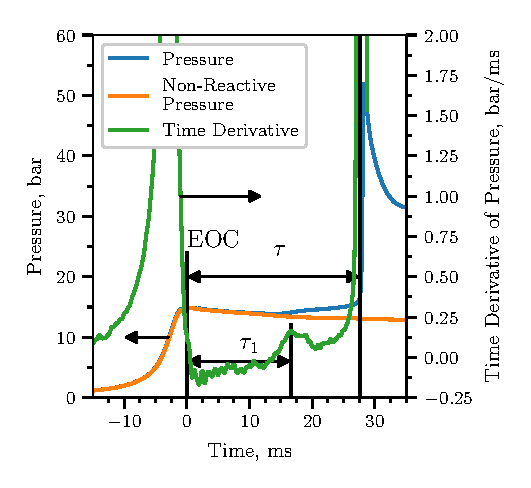
\includegraphics{figures/ignition_delay_definition.pdf}
    \caption{Definition of the ignition delays used in this work. The
    experiment in this figure was conducted for a \(\phi=2.0\) mixture with
    \mbox{\(\ce{Ar}/(\ce{N2}+\ce{AR})=0.5\)}, \(P_0=\SI{0.7806}{\bar}\),
    \(T_0=\SI{373}{\K}\), \(P_C=\SI{14.92}{\bar}\), \(T_C=\SI{720}{\K}\),
    \(\tau=\SI{27.56\pm0.89}{\ms}\), \(\tau_1=\SI{16.60\pm0.46}{\ms}\).}
    \label{fig:ign-delay-def}
\end{center}

In addition to the reactive experiments, non-reactive experiments are conducted to determine the
influence of machine-specific behavior on the experimental conditions and permit the calculation of
the EOC temperature via the isentropic relations between pressure and temperature~\cite{Lee1998}.
The EOC temperature is calculated by the procedure described in \cref{sec:computational-methods}.

The mixtures considered in this study are shown in \cref{tab:mixtures}. Four equivalence ratios of
MV in ``air'' are considered. The ratio of \(\ce{Ar}:\ce{N2}\) in the oxidizer is varied to adjust
the temperatures reached at the EOC for a given mixture. Two \(P_C\) conditions are studied in this
work, \SIlist{15;30}{\bar}, representing engine-relevant conditions. For the \(\phi=2.0\) condition,
only \(P_C = \SI{15}{\bar}\) is considered because we could not achieve \(T_C\) values low enough
that the ignition was long enough to be measured in our apparatus (the typical lower limit of
ignition delay on the present RCM is approximately \SI{5}{\ms}).

Mixtures are prepared in stainless steel mixing tanks, approximately \SI{17}{\L} and \SI{15}{\L} in
size. The proportions of reactants in the mixture are determined by specifying the absolute mass of
the fuel, the equivalence ratio \((\phi)\), and the ratio of \(\ce{Ar}:\ce{N2}\) in the oxidizer.
Mixtures are made by first vacuuming the mixing tanks to an ultimate pressure less than
\SI{5}{\torr}. Since MV is a liquid with a relatively small vapor pressure at room temperature and
pressure, it is measured gravimetrically in a syringe to within \SI{0.01}{\g} of the specified
value. The fuel is injected into the mixing tank through a septum. Proportions of \ce{O2}, \ce{Ar},
and \ce{N2} are added manometrically at room temperature and the total pressure is measured by an
Omega Engineering MMA type static pressure transducer. The same transducer is used to measure the
pressure of the reactants prior to an experiment.

\begin{center}
    \captionsetup{type=table}
    \caption{Mixtures considered in this work}
    \begin{tabular}{Sccccc}
        \toprule
        {\(\phi\)} & \multicolumn{4}{c}{Mole Fraction (purity)} & \ce{Ar}/(\ce{N2} + \ce{Ar}) \\
        \cmidrule{2-5}
         & \ce{MV} (\SI{100}{\percent}) & \ce{O2} (\SI{99.994}{\percent}) & \ce{Ar} (\SI{99.999}{\percent}) & \ce{N2} (\SI{99.999}{\percent}) &  \\
        \midrule
        0.25 & 0.0065 & 0.2087 & 0.7848 & 0.0000 & 1.0 \\
        0.5 & 0.0130 & 0.2074 & 0.7798 & 0.0000 & 1.0 \\
        1.0 & 0.0256 & 0.2047 & 0.7697 & 0.0000 & 1.0 \\
        1.0 & 0.0256 & 0.2047 & 0.3849 & 0.3848 & 0.5 \\
        2.0 & 0.0499 & 0.1996 & 0.0000 & 0.7505 & 0.0 \\
        2.0 & 0.0499 & 0.1996 & 0.3752 & 0.3753 & 0.5 \\
        \bottomrule
    \end{tabular}
    \label{tab:mixtures}
\end{center}

The RCM is equipped with heaters to control the initial temperature of the mixture. After filling in
the components to the mixing tanks, the heaters are switched on and the system is allowed
\SI{1.5}{\hour} to come to steady state. The mixing tanks are also equipped with magnetic stir bars
so the reactants are well mixed for the duration of the experiments.

The initial temperature is chosen such that the saturated vapor pressure \((P_{\text{sat}})\) of the
fuel at the initial temperature is at least twice the partial pressure of the fuel in the mixing
tank. The Antoine equation
%
\begin{equation}\label{eq:antoine}
    \logten{P_{\text{sat}}} = A - \frac{B}{T - C}
\end{equation}
%
is used to model the saturated vapor pressure of MV as a function of temperature, where \(A\),
\(B\), and \(C\) are substance-specific coefficients. Coefficients for \cref{eq:antoine} are given
in the literature by~\citet{Ortega2003}, \citet{Camacho2007}, and~\citet{Stephenson1987}.
Unfortunately, the values of the coefficients are different among all three authors and, more
importantly, the temperature ranges provided in those three fits do not cover the entire range of
interest for this study. Therefore, coefficients for use in \cref{eq:antoine} are determined in this
work by least squares fitting of the data of \citet{Ortega2003}, \citet{vanGenderen2002}, and
\citet{Verevkin2008} using the \verb|curve_fit()| function of SciPy~\cite{Jones2001} version 0.19.0.
\Cref{fig:vapor-pressure} shows that the coefficients fit with this procedure give good agreement
with the experimental data; values for the coefficients computed in this work and in the literature
works are given in \cref{tab:antoine}. The data used to calculate the coefficients are provided in
the Supplementary Material.

\begin{center}
    \captionsetup{type=figure}
    %% Creator: Matplotlib, PGF backend
%%
%% To include the figure in your LaTeX document, write
%%   \input{<filename>.pgf}
%%
%% Make sure the required packages are loaded in your preamble
%%   \usepackage{pgf}
%%
%% Figures using additional raster images can only be included by \input if
%% they are in the same directory as the main LaTeX file. For loading figures
%% from other directories you can use the `import` package
%%   \usepackage{import}
%% and then include the figures with
%%   \import{<path to file>}{<filename>.pgf}
%%
%% Matplotlib used the following preamble
%%   \usepackage{mathtools}
%%
\begingroup%
\makeatletter%
\begin{pgfpicture}%
\pgfpathrectangle{\pgfpointorigin}{\pgfqpoint{3.543307in}{3.000000in}}%
\pgfusepath{use as bounding box, clip}%
\begin{pgfscope}%
\pgfsetbuttcap%
\pgfsetmiterjoin%
\definecolor{currentfill}{rgb}{1.000000,1.000000,1.000000}%
\pgfsetfillcolor{currentfill}%
\pgfsetlinewidth{0.000000pt}%
\definecolor{currentstroke}{rgb}{1.000000,1.000000,1.000000}%
\pgfsetstrokecolor{currentstroke}%
\pgfsetdash{}{0pt}%
\pgfpathmoveto{\pgfqpoint{0.000000in}{0.000000in}}%
\pgfpathlineto{\pgfqpoint{3.543307in}{0.000000in}}%
\pgfpathlineto{\pgfqpoint{3.543307in}{3.000000in}}%
\pgfpathlineto{\pgfqpoint{0.000000in}{3.000000in}}%
\pgfpathclose%
\pgfusepath{fill}%
\end{pgfscope}%
\begin{pgfscope}%
\pgfsetbuttcap%
\pgfsetmiterjoin%
\definecolor{currentfill}{rgb}{1.000000,1.000000,1.000000}%
\pgfsetfillcolor{currentfill}%
\pgfsetlinewidth{0.000000pt}%
\definecolor{currentstroke}{rgb}{0.000000,0.000000,0.000000}%
\pgfsetstrokecolor{currentstroke}%
\pgfsetstrokeopacity{0.000000}%
\pgfsetdash{}{0pt}%
\pgfpathmoveto{\pgfqpoint{0.715877in}{0.602068in}}%
\pgfpathlineto{\pgfqpoint{3.313307in}{0.602068in}}%
\pgfpathlineto{\pgfqpoint{3.313307in}{2.770000in}}%
\pgfpathlineto{\pgfqpoint{0.715877in}{2.770000in}}%
\pgfpathclose%
\pgfusepath{fill}%
\end{pgfscope}%
\begin{pgfscope}%
\pgfpathrectangle{\pgfqpoint{0.715877in}{0.602068in}}{\pgfqpoint{2.597430in}{2.167932in}} %
\pgfusepath{clip}%
\pgfsetbuttcap%
\pgfsetroundjoin%
\definecolor{currentfill}{rgb}{0.839216,0.152941,0.156863}%
\pgfsetfillcolor{currentfill}%
\pgfsetfillopacity{0.250000}%
\pgfsetlinewidth{0.000000pt}%
\definecolor{currentstroke}{rgb}{0.000000,0.000000,0.000000}%
\pgfsetstrokecolor{currentstroke}%
\pgfsetdash{}{0pt}%
\pgfpathmoveto{\pgfqpoint{0.780813in}{1.255774in}}%
\pgfpathlineto{\pgfqpoint{0.780813in}{0.889342in}}%
\pgfpathlineto{\pgfqpoint{0.797047in}{0.909624in}}%
\pgfpathlineto{\pgfqpoint{0.813281in}{0.929719in}}%
\pgfpathlineto{\pgfqpoint{0.829515in}{0.949630in}}%
\pgfpathlineto{\pgfqpoint{0.845749in}{0.969361in}}%
\pgfpathlineto{\pgfqpoint{0.861983in}{0.988914in}}%
\pgfpathlineto{\pgfqpoint{0.878216in}{1.008290in}}%
\pgfpathlineto{\pgfqpoint{0.894450in}{1.027493in}}%
\pgfpathlineto{\pgfqpoint{0.910684in}{1.046525in}}%
\pgfpathlineto{\pgfqpoint{0.926918in}{1.065387in}}%
\pgfpathlineto{\pgfqpoint{0.943152in}{1.084083in}}%
\pgfpathlineto{\pgfqpoint{0.959386in}{1.102614in}}%
\pgfpathlineto{\pgfqpoint{0.975620in}{1.120983in}}%
\pgfpathlineto{\pgfqpoint{0.991854in}{1.139191in}}%
\pgfpathlineto{\pgfqpoint{1.008088in}{1.157242in}}%
\pgfpathlineto{\pgfqpoint{1.024322in}{1.175136in}}%
\pgfpathlineto{\pgfqpoint{1.040556in}{1.192876in}}%
\pgfpathlineto{\pgfqpoint{1.056790in}{1.210463in}}%
\pgfpathlineto{\pgfqpoint{1.073024in}{1.227901in}}%
\pgfpathlineto{\pgfqpoint{1.089258in}{1.245190in}}%
\pgfpathlineto{\pgfqpoint{1.105492in}{1.262333in}}%
\pgfpathlineto{\pgfqpoint{1.121726in}{1.279332in}}%
\pgfpathlineto{\pgfqpoint{1.137959in}{1.296187in}}%
\pgfpathlineto{\pgfqpoint{1.154193in}{1.312902in}}%
\pgfpathlineto{\pgfqpoint{1.170427in}{1.329477in}}%
\pgfpathlineto{\pgfqpoint{1.186661in}{1.345915in}}%
\pgfpathlineto{\pgfqpoint{1.202895in}{1.362218in}}%
\pgfpathlineto{\pgfqpoint{1.219129in}{1.378386in}}%
\pgfpathlineto{\pgfqpoint{1.235363in}{1.394422in}}%
\pgfpathlineto{\pgfqpoint{1.251597in}{1.410327in}}%
\pgfpathlineto{\pgfqpoint{1.267831in}{1.426102in}}%
\pgfpathlineto{\pgfqpoint{1.284065in}{1.441750in}}%
\pgfpathlineto{\pgfqpoint{1.300299in}{1.457272in}}%
\pgfpathlineto{\pgfqpoint{1.316533in}{1.472670in}}%
\pgfpathlineto{\pgfqpoint{1.332767in}{1.487944in}}%
\pgfpathlineto{\pgfqpoint{1.349001in}{1.503097in}}%
\pgfpathlineto{\pgfqpoint{1.365235in}{1.518130in}}%
\pgfpathlineto{\pgfqpoint{1.381469in}{1.533043in}}%
\pgfpathlineto{\pgfqpoint{1.397702in}{1.547840in}}%
\pgfpathlineto{\pgfqpoint{1.413936in}{1.562520in}}%
\pgfpathlineto{\pgfqpoint{1.430170in}{1.577086in}}%
\pgfpathlineto{\pgfqpoint{1.446404in}{1.591539in}}%
\pgfpathlineto{\pgfqpoint{1.462638in}{1.605880in}}%
\pgfpathlineto{\pgfqpoint{1.478872in}{1.620110in}}%
\pgfpathlineto{\pgfqpoint{1.495106in}{1.634230in}}%
\pgfpathlineto{\pgfqpoint{1.511340in}{1.648243in}}%
\pgfpathlineto{\pgfqpoint{1.527574in}{1.662148in}}%
\pgfpathlineto{\pgfqpoint{1.543808in}{1.675948in}}%
\pgfpathlineto{\pgfqpoint{1.560042in}{1.689644in}}%
\pgfpathlineto{\pgfqpoint{1.576276in}{1.703236in}}%
\pgfpathlineto{\pgfqpoint{1.592510in}{1.716726in}}%
\pgfpathlineto{\pgfqpoint{1.608744in}{1.730115in}}%
\pgfpathlineto{\pgfqpoint{1.624978in}{1.743404in}}%
\pgfpathlineto{\pgfqpoint{1.641212in}{1.756595in}}%
\pgfpathlineto{\pgfqpoint{1.657445in}{1.769687in}}%
\pgfpathlineto{\pgfqpoint{1.673679in}{1.782684in}}%
\pgfpathlineto{\pgfqpoint{1.689913in}{1.795584in}}%
\pgfpathlineto{\pgfqpoint{1.706147in}{1.808391in}}%
\pgfpathlineto{\pgfqpoint{1.722381in}{1.821104in}}%
\pgfpathlineto{\pgfqpoint{1.738615in}{1.833724in}}%
\pgfpathlineto{\pgfqpoint{1.754849in}{1.846253in}}%
\pgfpathlineto{\pgfqpoint{1.771083in}{1.858692in}}%
\pgfpathlineto{\pgfqpoint{1.787317in}{1.871041in}}%
\pgfpathlineto{\pgfqpoint{1.803551in}{1.883302in}}%
\pgfpathlineto{\pgfqpoint{1.819785in}{1.895476in}}%
\pgfpathlineto{\pgfqpoint{1.836019in}{1.907562in}}%
\pgfpathlineto{\pgfqpoint{1.852253in}{1.919563in}}%
\pgfpathlineto{\pgfqpoint{1.868487in}{1.931480in}}%
\pgfpathlineto{\pgfqpoint{1.884721in}{1.943312in}}%
\pgfpathlineto{\pgfqpoint{1.900955in}{1.955062in}}%
\pgfpathlineto{\pgfqpoint{1.917188in}{1.966729in}}%
\pgfpathlineto{\pgfqpoint{1.933422in}{1.978315in}}%
\pgfpathlineto{\pgfqpoint{1.949656in}{1.989821in}}%
\pgfpathlineto{\pgfqpoint{1.965890in}{2.001247in}}%
\pgfpathlineto{\pgfqpoint{1.982124in}{2.012594in}}%
\pgfpathlineto{\pgfqpoint{1.998358in}{2.023864in}}%
\pgfpathlineto{\pgfqpoint{2.014592in}{2.035056in}}%
\pgfpathlineto{\pgfqpoint{2.030826in}{2.046172in}}%
\pgfpathlineto{\pgfqpoint{2.047060in}{2.057212in}}%
\pgfpathlineto{\pgfqpoint{2.063294in}{2.068178in}}%
\pgfpathlineto{\pgfqpoint{2.079528in}{2.079069in}}%
\pgfpathlineto{\pgfqpoint{2.095762in}{2.089888in}}%
\pgfpathlineto{\pgfqpoint{2.111996in}{2.100633in}}%
\pgfpathlineto{\pgfqpoint{2.128230in}{2.111307in}}%
\pgfpathlineto{\pgfqpoint{2.144464in}{2.121910in}}%
\pgfpathlineto{\pgfqpoint{2.160698in}{2.132442in}}%
\pgfpathlineto{\pgfqpoint{2.176931in}{2.142905in}}%
\pgfpathlineto{\pgfqpoint{2.193165in}{2.153298in}}%
\pgfpathlineto{\pgfqpoint{2.209399in}{2.163623in}}%
\pgfpathlineto{\pgfqpoint{2.225633in}{2.173881in}}%
\pgfpathlineto{\pgfqpoint{2.241867in}{2.184072in}}%
\pgfpathlineto{\pgfqpoint{2.258101in}{2.194196in}}%
\pgfpathlineto{\pgfqpoint{2.274335in}{2.204254in}}%
\pgfpathlineto{\pgfqpoint{2.290569in}{2.214248in}}%
\pgfpathlineto{\pgfqpoint{2.306803in}{2.224177in}}%
\pgfpathlineto{\pgfqpoint{2.323037in}{2.234042in}}%
\pgfpathlineto{\pgfqpoint{2.339271in}{2.243844in}}%
\pgfpathlineto{\pgfqpoint{2.355505in}{2.253583in}}%
\pgfpathlineto{\pgfqpoint{2.371739in}{2.263261in}}%
\pgfpathlineto{\pgfqpoint{2.387973in}{2.272877in}}%
\pgfpathlineto{\pgfqpoint{2.404207in}{2.282432in}}%
\pgfpathlineto{\pgfqpoint{2.420441in}{2.291927in}}%
\pgfpathlineto{\pgfqpoint{2.436674in}{2.301362in}}%
\pgfpathlineto{\pgfqpoint{2.452908in}{2.310738in}}%
\pgfpathlineto{\pgfqpoint{2.469142in}{2.320056in}}%
\pgfpathlineto{\pgfqpoint{2.485376in}{2.329315in}}%
\pgfpathlineto{\pgfqpoint{2.501610in}{2.338518in}}%
\pgfpathlineto{\pgfqpoint{2.517844in}{2.347663in}}%
\pgfpathlineto{\pgfqpoint{2.534078in}{2.356751in}}%
\pgfpathlineto{\pgfqpoint{2.550312in}{2.365784in}}%
\pgfpathlineto{\pgfqpoint{2.566546in}{2.374762in}}%
\pgfpathlineto{\pgfqpoint{2.582780in}{2.383684in}}%
\pgfpathlineto{\pgfqpoint{2.599014in}{2.392552in}}%
\pgfpathlineto{\pgfqpoint{2.615248in}{2.401367in}}%
\pgfpathlineto{\pgfqpoint{2.631482in}{2.410127in}}%
\pgfpathlineto{\pgfqpoint{2.647716in}{2.418835in}}%
\pgfpathlineto{\pgfqpoint{2.663950in}{2.427491in}}%
\pgfpathlineto{\pgfqpoint{2.680184in}{2.436095in}}%
\pgfpathlineto{\pgfqpoint{2.696417in}{2.444647in}}%
\pgfpathlineto{\pgfqpoint{2.712651in}{2.453148in}}%
\pgfpathlineto{\pgfqpoint{2.728885in}{2.461598in}}%
\pgfpathlineto{\pgfqpoint{2.745119in}{2.469999in}}%
\pgfpathlineto{\pgfqpoint{2.761353in}{2.478349in}}%
\pgfpathlineto{\pgfqpoint{2.777587in}{2.486651in}}%
\pgfpathlineto{\pgfqpoint{2.793821in}{2.494904in}}%
\pgfpathlineto{\pgfqpoint{2.810055in}{2.503108in}}%
\pgfpathlineto{\pgfqpoint{2.826289in}{2.511264in}}%
\pgfpathlineto{\pgfqpoint{2.842523in}{2.519373in}}%
\pgfpathlineto{\pgfqpoint{2.858757in}{2.527435in}}%
\pgfpathlineto{\pgfqpoint{2.874991in}{2.535450in}}%
\pgfpathlineto{\pgfqpoint{2.891225in}{2.543418in}}%
\pgfpathlineto{\pgfqpoint{2.907459in}{2.551341in}}%
\pgfpathlineto{\pgfqpoint{2.923693in}{2.559218in}}%
\pgfpathlineto{\pgfqpoint{2.939927in}{2.567050in}}%
\pgfpathlineto{\pgfqpoint{2.956160in}{2.574838in}}%
\pgfpathlineto{\pgfqpoint{2.972394in}{2.582581in}}%
\pgfpathlineto{\pgfqpoint{2.988628in}{2.590280in}}%
\pgfpathlineto{\pgfqpoint{3.004862in}{2.597935in}}%
\pgfpathlineto{\pgfqpoint{3.021096in}{2.605548in}}%
\pgfpathlineto{\pgfqpoint{3.037330in}{2.613117in}}%
\pgfpathlineto{\pgfqpoint{3.053564in}{2.620644in}}%
\pgfpathlineto{\pgfqpoint{3.069798in}{2.628129in}}%
\pgfpathlineto{\pgfqpoint{3.086032in}{2.635572in}}%
\pgfpathlineto{\pgfqpoint{3.102266in}{2.642973in}}%
\pgfpathlineto{\pgfqpoint{3.102266in}{2.777687in}}%
\pgfpathlineto{\pgfqpoint{3.102266in}{2.777687in}}%
\pgfpathlineto{\pgfqpoint{3.086032in}{2.771150in}}%
\pgfpathlineto{\pgfqpoint{3.069798in}{2.764578in}}%
\pgfpathlineto{\pgfqpoint{3.053564in}{2.757970in}}%
\pgfpathlineto{\pgfqpoint{3.037330in}{2.751326in}}%
\pgfpathlineto{\pgfqpoint{3.021096in}{2.744645in}}%
\pgfpathlineto{\pgfqpoint{3.004862in}{2.737927in}}%
\pgfpathlineto{\pgfqpoint{2.988628in}{2.731172in}}%
\pgfpathlineto{\pgfqpoint{2.972394in}{2.724380in}}%
\pgfpathlineto{\pgfqpoint{2.956160in}{2.717550in}}%
\pgfpathlineto{\pgfqpoint{2.939927in}{2.710682in}}%
\pgfpathlineto{\pgfqpoint{2.923693in}{2.703776in}}%
\pgfpathlineto{\pgfqpoint{2.907459in}{2.696831in}}%
\pgfpathlineto{\pgfqpoint{2.891225in}{2.689847in}}%
\pgfpathlineto{\pgfqpoint{2.874991in}{2.682824in}}%
\pgfpathlineto{\pgfqpoint{2.858757in}{2.675761in}}%
\pgfpathlineto{\pgfqpoint{2.842523in}{2.668658in}}%
\pgfpathlineto{\pgfqpoint{2.826289in}{2.661514in}}%
\pgfpathlineto{\pgfqpoint{2.810055in}{2.654330in}}%
\pgfpathlineto{\pgfqpoint{2.793821in}{2.647105in}}%
\pgfpathlineto{\pgfqpoint{2.777587in}{2.639838in}}%
\pgfpathlineto{\pgfqpoint{2.761353in}{2.632530in}}%
\pgfpathlineto{\pgfqpoint{2.745119in}{2.625180in}}%
\pgfpathlineto{\pgfqpoint{2.728885in}{2.617787in}}%
\pgfpathlineto{\pgfqpoint{2.712651in}{2.610351in}}%
\pgfpathlineto{\pgfqpoint{2.696417in}{2.602872in}}%
\pgfpathlineto{\pgfqpoint{2.680184in}{2.595350in}}%
\pgfpathlineto{\pgfqpoint{2.663950in}{2.587783in}}%
\pgfpathlineto{\pgfqpoint{2.647716in}{2.580172in}}%
\pgfpathlineto{\pgfqpoint{2.631482in}{2.572517in}}%
\pgfpathlineto{\pgfqpoint{2.615248in}{2.564816in}}%
\pgfpathlineto{\pgfqpoint{2.599014in}{2.557069in}}%
\pgfpathlineto{\pgfqpoint{2.582780in}{2.549277in}}%
\pgfpathlineto{\pgfqpoint{2.566546in}{2.541438in}}%
\pgfpathlineto{\pgfqpoint{2.550312in}{2.533553in}}%
\pgfpathlineto{\pgfqpoint{2.534078in}{2.525620in}}%
\pgfpathlineto{\pgfqpoint{2.517844in}{2.517639in}}%
\pgfpathlineto{\pgfqpoint{2.501610in}{2.509611in}}%
\pgfpathlineto{\pgfqpoint{2.485376in}{2.501534in}}%
\pgfpathlineto{\pgfqpoint{2.469142in}{2.493408in}}%
\pgfpathlineto{\pgfqpoint{2.452908in}{2.485233in}}%
\pgfpathlineto{\pgfqpoint{2.436674in}{2.477008in}}%
\pgfpathlineto{\pgfqpoint{2.420441in}{2.468732in}}%
\pgfpathlineto{\pgfqpoint{2.404207in}{2.460406in}}%
\pgfpathlineto{\pgfqpoint{2.387973in}{2.452029in}}%
\pgfpathlineto{\pgfqpoint{2.371739in}{2.443600in}}%
\pgfpathlineto{\pgfqpoint{2.355505in}{2.435118in}}%
\pgfpathlineto{\pgfqpoint{2.339271in}{2.426584in}}%
\pgfpathlineto{\pgfqpoint{2.323037in}{2.417997in}}%
\pgfpathlineto{\pgfqpoint{2.306803in}{2.409356in}}%
\pgfpathlineto{\pgfqpoint{2.290569in}{2.400661in}}%
\pgfpathlineto{\pgfqpoint{2.274335in}{2.391912in}}%
\pgfpathlineto{\pgfqpoint{2.258101in}{2.383107in}}%
\pgfpathlineto{\pgfqpoint{2.241867in}{2.374246in}}%
\pgfpathlineto{\pgfqpoint{2.225633in}{2.365330in}}%
\pgfpathlineto{\pgfqpoint{2.209399in}{2.356356in}}%
\pgfpathlineto{\pgfqpoint{2.193165in}{2.347325in}}%
\pgfpathlineto{\pgfqpoint{2.176931in}{2.338236in}}%
\pgfpathlineto{\pgfqpoint{2.160698in}{2.329089in}}%
\pgfpathlineto{\pgfqpoint{2.144464in}{2.319883in}}%
\pgfpathlineto{\pgfqpoint{2.128230in}{2.310617in}}%
\pgfpathlineto{\pgfqpoint{2.111996in}{2.301291in}}%
\pgfpathlineto{\pgfqpoint{2.095762in}{2.291904in}}%
\pgfpathlineto{\pgfqpoint{2.079528in}{2.282456in}}%
\pgfpathlineto{\pgfqpoint{2.063294in}{2.272946in}}%
\pgfpathlineto{\pgfqpoint{2.047060in}{2.263374in}}%
\pgfpathlineto{\pgfqpoint{2.030826in}{2.253738in}}%
\pgfpathlineto{\pgfqpoint{2.014592in}{2.244038in}}%
\pgfpathlineto{\pgfqpoint{1.998358in}{2.234274in}}%
\pgfpathlineto{\pgfqpoint{1.982124in}{2.224445in}}%
\pgfpathlineto{\pgfqpoint{1.965890in}{2.214551in}}%
\pgfpathlineto{\pgfqpoint{1.949656in}{2.204589in}}%
\pgfpathlineto{\pgfqpoint{1.933422in}{2.194561in}}%
\pgfpathlineto{\pgfqpoint{1.917188in}{2.184465in}}%
\pgfpathlineto{\pgfqpoint{1.900955in}{2.174301in}}%
\pgfpathlineto{\pgfqpoint{1.884721in}{2.164067in}}%
\pgfpathlineto{\pgfqpoint{1.868487in}{2.153764in}}%
\pgfpathlineto{\pgfqpoint{1.852253in}{2.143390in}}%
\pgfpathlineto{\pgfqpoint{1.836019in}{2.132945in}}%
\pgfpathlineto{\pgfqpoint{1.819785in}{2.122427in}}%
\pgfpathlineto{\pgfqpoint{1.803551in}{2.111837in}}%
\pgfpathlineto{\pgfqpoint{1.787317in}{2.101174in}}%
\pgfpathlineto{\pgfqpoint{1.771083in}{2.090436in}}%
\pgfpathlineto{\pgfqpoint{1.754849in}{2.079623in}}%
\pgfpathlineto{\pgfqpoint{1.738615in}{2.068734in}}%
\pgfpathlineto{\pgfqpoint{1.722381in}{2.057769in}}%
\pgfpathlineto{\pgfqpoint{1.706147in}{2.046726in}}%
\pgfpathlineto{\pgfqpoint{1.689913in}{2.035604in}}%
\pgfpathlineto{\pgfqpoint{1.673679in}{2.024404in}}%
\pgfpathlineto{\pgfqpoint{1.657445in}{2.013124in}}%
\pgfpathlineto{\pgfqpoint{1.641212in}{2.001762in}}%
\pgfpathlineto{\pgfqpoint{1.624978in}{1.990319in}}%
\pgfpathlineto{\pgfqpoint{1.608744in}{1.978794in}}%
\pgfpathlineto{\pgfqpoint{1.592510in}{1.967185in}}%
\pgfpathlineto{\pgfqpoint{1.576276in}{1.955491in}}%
\pgfpathlineto{\pgfqpoint{1.560042in}{1.943712in}}%
\pgfpathlineto{\pgfqpoint{1.543808in}{1.931847in}}%
\pgfpathlineto{\pgfqpoint{1.527574in}{1.919895in}}%
\pgfpathlineto{\pgfqpoint{1.511340in}{1.907854in}}%
\pgfpathlineto{\pgfqpoint{1.495106in}{1.895725in}}%
\pgfpathlineto{\pgfqpoint{1.478872in}{1.883505in}}%
\pgfpathlineto{\pgfqpoint{1.462638in}{1.871194in}}%
\pgfpathlineto{\pgfqpoint{1.446404in}{1.858791in}}%
\pgfpathlineto{\pgfqpoint{1.430170in}{1.846294in}}%
\pgfpathlineto{\pgfqpoint{1.413936in}{1.833703in}}%
\pgfpathlineto{\pgfqpoint{1.397702in}{1.821017in}}%
\pgfpathlineto{\pgfqpoint{1.381469in}{1.808235in}}%
\pgfpathlineto{\pgfqpoint{1.365235in}{1.795355in}}%
\pgfpathlineto{\pgfqpoint{1.349001in}{1.782376in}}%
\pgfpathlineto{\pgfqpoint{1.332767in}{1.769297in}}%
\pgfpathlineto{\pgfqpoint{1.316533in}{1.756117in}}%
\pgfpathlineto{\pgfqpoint{1.300299in}{1.742836in}}%
\pgfpathlineto{\pgfqpoint{1.284065in}{1.729451in}}%
\pgfpathlineto{\pgfqpoint{1.267831in}{1.715961in}}%
\pgfpathlineto{\pgfqpoint{1.251597in}{1.702366in}}%
\pgfpathlineto{\pgfqpoint{1.235363in}{1.688663in}}%
\pgfpathlineto{\pgfqpoint{1.219129in}{1.674852in}}%
\pgfpathlineto{\pgfqpoint{1.202895in}{1.660932in}}%
\pgfpathlineto{\pgfqpoint{1.186661in}{1.646901in}}%
\pgfpathlineto{\pgfqpoint{1.170427in}{1.632757in}}%
\pgfpathlineto{\pgfqpoint{1.154193in}{1.618500in}}%
\pgfpathlineto{\pgfqpoint{1.137959in}{1.604128in}}%
\pgfpathlineto{\pgfqpoint{1.121726in}{1.589640in}}%
\pgfpathlineto{\pgfqpoint{1.105492in}{1.575034in}}%
\pgfpathlineto{\pgfqpoint{1.089258in}{1.560309in}}%
\pgfpathlineto{\pgfqpoint{1.073024in}{1.545463in}}%
\pgfpathlineto{\pgfqpoint{1.056790in}{1.530494in}}%
\pgfpathlineto{\pgfqpoint{1.040556in}{1.515403in}}%
\pgfpathlineto{\pgfqpoint{1.024322in}{1.500186in}}%
\pgfpathlineto{\pgfqpoint{1.008088in}{1.484842in}}%
\pgfpathlineto{\pgfqpoint{0.991854in}{1.469370in}}%
\pgfpathlineto{\pgfqpoint{0.975620in}{1.453767in}}%
\pgfpathlineto{\pgfqpoint{0.959386in}{1.438034in}}%
\pgfpathlineto{\pgfqpoint{0.943152in}{1.422167in}}%
\pgfpathlineto{\pgfqpoint{0.926918in}{1.406164in}}%
\pgfpathlineto{\pgfqpoint{0.910684in}{1.390026in}}%
\pgfpathlineto{\pgfqpoint{0.894450in}{1.373748in}}%
\pgfpathlineto{\pgfqpoint{0.878216in}{1.357330in}}%
\pgfpathlineto{\pgfqpoint{0.861983in}{1.340771in}}%
\pgfpathlineto{\pgfqpoint{0.845749in}{1.324067in}}%
\pgfpathlineto{\pgfqpoint{0.829515in}{1.307217in}}%
\pgfpathlineto{\pgfqpoint{0.813281in}{1.290220in}}%
\pgfpathlineto{\pgfqpoint{0.797047in}{1.273073in}}%
\pgfpathlineto{\pgfqpoint{0.780813in}{1.255774in}}%
\pgfpathclose%
\pgfusepath{fill}%
\end{pgfscope}%
\begin{pgfscope}%
\pgfsetbuttcap%
\pgfsetroundjoin%
\definecolor{currentfill}{rgb}{0.000000,0.000000,0.000000}%
\pgfsetfillcolor{currentfill}%
\pgfsetlinewidth{1.003750pt}%
\definecolor{currentstroke}{rgb}{0.000000,0.000000,0.000000}%
\pgfsetstrokecolor{currentstroke}%
\pgfsetdash{}{0pt}%
\pgfsys@defobject{currentmarker}{\pgfqpoint{0.000000in}{-0.069444in}}{\pgfqpoint{0.000000in}{0.000000in}}{%
\pgfpathmoveto{\pgfqpoint{0.000000in}{0.000000in}}%
\pgfpathlineto{\pgfqpoint{0.000000in}{-0.069444in}}%
\pgfusepath{stroke,fill}%
}%
\begin{pgfscope}%
\pgfsys@transformshift{0.715877in}{0.602068in}%
\pgfsys@useobject{currentmarker}{}%
\end{pgfscope}%
\end{pgfscope}%
\begin{pgfscope}%
\pgftext[x=0.715877in,y=0.484012in,,top]{\rmfamily\fontsize{9.000000}{10.800000}\selectfont \(\displaystyle 270\)}%
\end{pgfscope}%
\begin{pgfscope}%
\pgfsetbuttcap%
\pgfsetroundjoin%
\definecolor{currentfill}{rgb}{0.000000,0.000000,0.000000}%
\pgfsetfillcolor{currentfill}%
\pgfsetlinewidth{1.003750pt}%
\definecolor{currentstroke}{rgb}{0.000000,0.000000,0.000000}%
\pgfsetstrokecolor{currentstroke}%
\pgfsetdash{}{0pt}%
\pgfsys@defobject{currentmarker}{\pgfqpoint{0.000000in}{-0.069444in}}{\pgfqpoint{0.000000in}{0.000000in}}{%
\pgfpathmoveto{\pgfqpoint{0.000000in}{0.000000in}}%
\pgfpathlineto{\pgfqpoint{0.000000in}{-0.069444in}}%
\pgfusepath{stroke,fill}%
}%
\begin{pgfscope}%
\pgfsys@transformshift{1.202895in}{0.602068in}%
\pgfsys@useobject{currentmarker}{}%
\end{pgfscope}%
\end{pgfscope}%
\begin{pgfscope}%
\pgftext[x=1.202895in,y=0.484012in,,top]{\rmfamily\fontsize{9.000000}{10.800000}\selectfont \(\displaystyle 300\)}%
\end{pgfscope}%
\begin{pgfscope}%
\pgfsetbuttcap%
\pgfsetroundjoin%
\definecolor{currentfill}{rgb}{0.000000,0.000000,0.000000}%
\pgfsetfillcolor{currentfill}%
\pgfsetlinewidth{1.003750pt}%
\definecolor{currentstroke}{rgb}{0.000000,0.000000,0.000000}%
\pgfsetstrokecolor{currentstroke}%
\pgfsetdash{}{0pt}%
\pgfsys@defobject{currentmarker}{\pgfqpoint{0.000000in}{-0.069444in}}{\pgfqpoint{0.000000in}{0.000000in}}{%
\pgfpathmoveto{\pgfqpoint{0.000000in}{0.000000in}}%
\pgfpathlineto{\pgfqpoint{0.000000in}{-0.069444in}}%
\pgfusepath{stroke,fill}%
}%
\begin{pgfscope}%
\pgfsys@transformshift{1.689913in}{0.602068in}%
\pgfsys@useobject{currentmarker}{}%
\end{pgfscope}%
\end{pgfscope}%
\begin{pgfscope}%
\pgftext[x=1.689913in,y=0.484012in,,top]{\rmfamily\fontsize{9.000000}{10.800000}\selectfont \(\displaystyle 330\)}%
\end{pgfscope}%
\begin{pgfscope}%
\pgfsetbuttcap%
\pgfsetroundjoin%
\definecolor{currentfill}{rgb}{0.000000,0.000000,0.000000}%
\pgfsetfillcolor{currentfill}%
\pgfsetlinewidth{1.003750pt}%
\definecolor{currentstroke}{rgb}{0.000000,0.000000,0.000000}%
\pgfsetstrokecolor{currentstroke}%
\pgfsetdash{}{0pt}%
\pgfsys@defobject{currentmarker}{\pgfqpoint{0.000000in}{-0.069444in}}{\pgfqpoint{0.000000in}{0.000000in}}{%
\pgfpathmoveto{\pgfqpoint{0.000000in}{0.000000in}}%
\pgfpathlineto{\pgfqpoint{0.000000in}{-0.069444in}}%
\pgfusepath{stroke,fill}%
}%
\begin{pgfscope}%
\pgfsys@transformshift{2.176931in}{0.602068in}%
\pgfsys@useobject{currentmarker}{}%
\end{pgfscope}%
\end{pgfscope}%
\begin{pgfscope}%
\pgftext[x=2.176931in,y=0.484012in,,top]{\rmfamily\fontsize{9.000000}{10.800000}\selectfont \(\displaystyle 360\)}%
\end{pgfscope}%
\begin{pgfscope}%
\pgfsetbuttcap%
\pgfsetroundjoin%
\definecolor{currentfill}{rgb}{0.000000,0.000000,0.000000}%
\pgfsetfillcolor{currentfill}%
\pgfsetlinewidth{1.003750pt}%
\definecolor{currentstroke}{rgb}{0.000000,0.000000,0.000000}%
\pgfsetstrokecolor{currentstroke}%
\pgfsetdash{}{0pt}%
\pgfsys@defobject{currentmarker}{\pgfqpoint{0.000000in}{-0.069444in}}{\pgfqpoint{0.000000in}{0.000000in}}{%
\pgfpathmoveto{\pgfqpoint{0.000000in}{0.000000in}}%
\pgfpathlineto{\pgfqpoint{0.000000in}{-0.069444in}}%
\pgfusepath{stroke,fill}%
}%
\begin{pgfscope}%
\pgfsys@transformshift{2.663950in}{0.602068in}%
\pgfsys@useobject{currentmarker}{}%
\end{pgfscope}%
\end{pgfscope}%
\begin{pgfscope}%
\pgftext[x=2.663950in,y=0.484012in,,top]{\rmfamily\fontsize{9.000000}{10.800000}\selectfont \(\displaystyle 390\)}%
\end{pgfscope}%
\begin{pgfscope}%
\pgfsetbuttcap%
\pgfsetroundjoin%
\definecolor{currentfill}{rgb}{0.000000,0.000000,0.000000}%
\pgfsetfillcolor{currentfill}%
\pgfsetlinewidth{1.003750pt}%
\definecolor{currentstroke}{rgb}{0.000000,0.000000,0.000000}%
\pgfsetstrokecolor{currentstroke}%
\pgfsetdash{}{0pt}%
\pgfsys@defobject{currentmarker}{\pgfqpoint{0.000000in}{-0.069444in}}{\pgfqpoint{0.000000in}{0.000000in}}{%
\pgfpathmoveto{\pgfqpoint{0.000000in}{0.000000in}}%
\pgfpathlineto{\pgfqpoint{0.000000in}{-0.069444in}}%
\pgfusepath{stroke,fill}%
}%
\begin{pgfscope}%
\pgfsys@transformshift{3.150968in}{0.602068in}%
\pgfsys@useobject{currentmarker}{}%
\end{pgfscope}%
\end{pgfscope}%
\begin{pgfscope}%
\pgftext[x=3.150968in,y=0.484012in,,top]{\rmfamily\fontsize{9.000000}{10.800000}\selectfont \(\displaystyle 420\)}%
\end{pgfscope}%
\begin{pgfscope}%
\pgfsetbuttcap%
\pgfsetroundjoin%
\definecolor{currentfill}{rgb}{0.000000,0.000000,0.000000}%
\pgfsetfillcolor{currentfill}%
\pgfsetlinewidth{1.003750pt}%
\definecolor{currentstroke}{rgb}{0.000000,0.000000,0.000000}%
\pgfsetstrokecolor{currentstroke}%
\pgfsetdash{}{0pt}%
\pgfsys@defobject{currentmarker}{\pgfqpoint{0.000000in}{-0.034722in}}{\pgfqpoint{0.000000in}{0.000000in}}{%
\pgfpathmoveto{\pgfqpoint{0.000000in}{0.000000in}}%
\pgfpathlineto{\pgfqpoint{0.000000in}{-0.034722in}}%
\pgfusepath{stroke,fill}%
}%
\begin{pgfscope}%
\pgfsys@transformshift{0.878216in}{0.602068in}%
\pgfsys@useobject{currentmarker}{}%
\end{pgfscope}%
\end{pgfscope}%
\begin{pgfscope}%
\pgfsetbuttcap%
\pgfsetroundjoin%
\definecolor{currentfill}{rgb}{0.000000,0.000000,0.000000}%
\pgfsetfillcolor{currentfill}%
\pgfsetlinewidth{1.003750pt}%
\definecolor{currentstroke}{rgb}{0.000000,0.000000,0.000000}%
\pgfsetstrokecolor{currentstroke}%
\pgfsetdash{}{0pt}%
\pgfsys@defobject{currentmarker}{\pgfqpoint{0.000000in}{-0.034722in}}{\pgfqpoint{0.000000in}{0.000000in}}{%
\pgfpathmoveto{\pgfqpoint{0.000000in}{0.000000in}}%
\pgfpathlineto{\pgfqpoint{0.000000in}{-0.034722in}}%
\pgfusepath{stroke,fill}%
}%
\begin{pgfscope}%
\pgfsys@transformshift{1.040556in}{0.602068in}%
\pgfsys@useobject{currentmarker}{}%
\end{pgfscope}%
\end{pgfscope}%
\begin{pgfscope}%
\pgfsetbuttcap%
\pgfsetroundjoin%
\definecolor{currentfill}{rgb}{0.000000,0.000000,0.000000}%
\pgfsetfillcolor{currentfill}%
\pgfsetlinewidth{1.003750pt}%
\definecolor{currentstroke}{rgb}{0.000000,0.000000,0.000000}%
\pgfsetstrokecolor{currentstroke}%
\pgfsetdash{}{0pt}%
\pgfsys@defobject{currentmarker}{\pgfqpoint{0.000000in}{-0.034722in}}{\pgfqpoint{0.000000in}{0.000000in}}{%
\pgfpathmoveto{\pgfqpoint{0.000000in}{0.000000in}}%
\pgfpathlineto{\pgfqpoint{0.000000in}{-0.034722in}}%
\pgfusepath{stroke,fill}%
}%
\begin{pgfscope}%
\pgfsys@transformshift{1.365235in}{0.602068in}%
\pgfsys@useobject{currentmarker}{}%
\end{pgfscope}%
\end{pgfscope}%
\begin{pgfscope}%
\pgfsetbuttcap%
\pgfsetroundjoin%
\definecolor{currentfill}{rgb}{0.000000,0.000000,0.000000}%
\pgfsetfillcolor{currentfill}%
\pgfsetlinewidth{1.003750pt}%
\definecolor{currentstroke}{rgb}{0.000000,0.000000,0.000000}%
\pgfsetstrokecolor{currentstroke}%
\pgfsetdash{}{0pt}%
\pgfsys@defobject{currentmarker}{\pgfqpoint{0.000000in}{-0.034722in}}{\pgfqpoint{0.000000in}{0.000000in}}{%
\pgfpathmoveto{\pgfqpoint{0.000000in}{0.000000in}}%
\pgfpathlineto{\pgfqpoint{0.000000in}{-0.034722in}}%
\pgfusepath{stroke,fill}%
}%
\begin{pgfscope}%
\pgfsys@transformshift{1.527574in}{0.602068in}%
\pgfsys@useobject{currentmarker}{}%
\end{pgfscope}%
\end{pgfscope}%
\begin{pgfscope}%
\pgfsetbuttcap%
\pgfsetroundjoin%
\definecolor{currentfill}{rgb}{0.000000,0.000000,0.000000}%
\pgfsetfillcolor{currentfill}%
\pgfsetlinewidth{1.003750pt}%
\definecolor{currentstroke}{rgb}{0.000000,0.000000,0.000000}%
\pgfsetstrokecolor{currentstroke}%
\pgfsetdash{}{0pt}%
\pgfsys@defobject{currentmarker}{\pgfqpoint{0.000000in}{-0.034722in}}{\pgfqpoint{0.000000in}{0.000000in}}{%
\pgfpathmoveto{\pgfqpoint{0.000000in}{0.000000in}}%
\pgfpathlineto{\pgfqpoint{0.000000in}{-0.034722in}}%
\pgfusepath{stroke,fill}%
}%
\begin{pgfscope}%
\pgfsys@transformshift{1.852253in}{0.602068in}%
\pgfsys@useobject{currentmarker}{}%
\end{pgfscope}%
\end{pgfscope}%
\begin{pgfscope}%
\pgfsetbuttcap%
\pgfsetroundjoin%
\definecolor{currentfill}{rgb}{0.000000,0.000000,0.000000}%
\pgfsetfillcolor{currentfill}%
\pgfsetlinewidth{1.003750pt}%
\definecolor{currentstroke}{rgb}{0.000000,0.000000,0.000000}%
\pgfsetstrokecolor{currentstroke}%
\pgfsetdash{}{0pt}%
\pgfsys@defobject{currentmarker}{\pgfqpoint{0.000000in}{-0.034722in}}{\pgfqpoint{0.000000in}{0.000000in}}{%
\pgfpathmoveto{\pgfqpoint{0.000000in}{0.000000in}}%
\pgfpathlineto{\pgfqpoint{0.000000in}{-0.034722in}}%
\pgfusepath{stroke,fill}%
}%
\begin{pgfscope}%
\pgfsys@transformshift{2.014592in}{0.602068in}%
\pgfsys@useobject{currentmarker}{}%
\end{pgfscope}%
\end{pgfscope}%
\begin{pgfscope}%
\pgfsetbuttcap%
\pgfsetroundjoin%
\definecolor{currentfill}{rgb}{0.000000,0.000000,0.000000}%
\pgfsetfillcolor{currentfill}%
\pgfsetlinewidth{1.003750pt}%
\definecolor{currentstroke}{rgb}{0.000000,0.000000,0.000000}%
\pgfsetstrokecolor{currentstroke}%
\pgfsetdash{}{0pt}%
\pgfsys@defobject{currentmarker}{\pgfqpoint{0.000000in}{-0.034722in}}{\pgfqpoint{0.000000in}{0.000000in}}{%
\pgfpathmoveto{\pgfqpoint{0.000000in}{0.000000in}}%
\pgfpathlineto{\pgfqpoint{0.000000in}{-0.034722in}}%
\pgfusepath{stroke,fill}%
}%
\begin{pgfscope}%
\pgfsys@transformshift{2.339271in}{0.602068in}%
\pgfsys@useobject{currentmarker}{}%
\end{pgfscope}%
\end{pgfscope}%
\begin{pgfscope}%
\pgfsetbuttcap%
\pgfsetroundjoin%
\definecolor{currentfill}{rgb}{0.000000,0.000000,0.000000}%
\pgfsetfillcolor{currentfill}%
\pgfsetlinewidth{1.003750pt}%
\definecolor{currentstroke}{rgb}{0.000000,0.000000,0.000000}%
\pgfsetstrokecolor{currentstroke}%
\pgfsetdash{}{0pt}%
\pgfsys@defobject{currentmarker}{\pgfqpoint{0.000000in}{-0.034722in}}{\pgfqpoint{0.000000in}{0.000000in}}{%
\pgfpathmoveto{\pgfqpoint{0.000000in}{0.000000in}}%
\pgfpathlineto{\pgfqpoint{0.000000in}{-0.034722in}}%
\pgfusepath{stroke,fill}%
}%
\begin{pgfscope}%
\pgfsys@transformshift{2.501610in}{0.602068in}%
\pgfsys@useobject{currentmarker}{}%
\end{pgfscope}%
\end{pgfscope}%
\begin{pgfscope}%
\pgfsetbuttcap%
\pgfsetroundjoin%
\definecolor{currentfill}{rgb}{0.000000,0.000000,0.000000}%
\pgfsetfillcolor{currentfill}%
\pgfsetlinewidth{1.003750pt}%
\definecolor{currentstroke}{rgb}{0.000000,0.000000,0.000000}%
\pgfsetstrokecolor{currentstroke}%
\pgfsetdash{}{0pt}%
\pgfsys@defobject{currentmarker}{\pgfqpoint{0.000000in}{-0.034722in}}{\pgfqpoint{0.000000in}{0.000000in}}{%
\pgfpathmoveto{\pgfqpoint{0.000000in}{0.000000in}}%
\pgfpathlineto{\pgfqpoint{0.000000in}{-0.034722in}}%
\pgfusepath{stroke,fill}%
}%
\begin{pgfscope}%
\pgfsys@transformshift{2.826289in}{0.602068in}%
\pgfsys@useobject{currentmarker}{}%
\end{pgfscope}%
\end{pgfscope}%
\begin{pgfscope}%
\pgfsetbuttcap%
\pgfsetroundjoin%
\definecolor{currentfill}{rgb}{0.000000,0.000000,0.000000}%
\pgfsetfillcolor{currentfill}%
\pgfsetlinewidth{1.003750pt}%
\definecolor{currentstroke}{rgb}{0.000000,0.000000,0.000000}%
\pgfsetstrokecolor{currentstroke}%
\pgfsetdash{}{0pt}%
\pgfsys@defobject{currentmarker}{\pgfqpoint{0.000000in}{-0.034722in}}{\pgfqpoint{0.000000in}{0.000000in}}{%
\pgfpathmoveto{\pgfqpoint{0.000000in}{0.000000in}}%
\pgfpathlineto{\pgfqpoint{0.000000in}{-0.034722in}}%
\pgfusepath{stroke,fill}%
}%
\begin{pgfscope}%
\pgfsys@transformshift{2.988628in}{0.602068in}%
\pgfsys@useobject{currentmarker}{}%
\end{pgfscope}%
\end{pgfscope}%
\begin{pgfscope}%
\pgfsetbuttcap%
\pgfsetroundjoin%
\definecolor{currentfill}{rgb}{0.000000,0.000000,0.000000}%
\pgfsetfillcolor{currentfill}%
\pgfsetlinewidth{1.003750pt}%
\definecolor{currentstroke}{rgb}{0.000000,0.000000,0.000000}%
\pgfsetstrokecolor{currentstroke}%
\pgfsetdash{}{0pt}%
\pgfsys@defobject{currentmarker}{\pgfqpoint{0.000000in}{-0.034722in}}{\pgfqpoint{0.000000in}{0.000000in}}{%
\pgfpathmoveto{\pgfqpoint{0.000000in}{0.000000in}}%
\pgfpathlineto{\pgfqpoint{0.000000in}{-0.034722in}}%
\pgfusepath{stroke,fill}%
}%
\begin{pgfscope}%
\pgfsys@transformshift{3.313307in}{0.602068in}%
\pgfsys@useobject{currentmarker}{}%
\end{pgfscope}%
\end{pgfscope}%
\begin{pgfscope}%
\pgftext[x=2.014592in,y=0.303457in,,top]{\rmfamily\fontsize{10.000000}{12.000000}\selectfont \(\displaystyle T\), K}%
\end{pgfscope}%
\begin{pgfscope}%
\pgfsetbuttcap%
\pgfsetroundjoin%
\definecolor{currentfill}{rgb}{0.000000,0.000000,0.000000}%
\pgfsetfillcolor{currentfill}%
\pgfsetlinewidth{1.003750pt}%
\definecolor{currentstroke}{rgb}{0.000000,0.000000,0.000000}%
\pgfsetstrokecolor{currentstroke}%
\pgfsetdash{}{0pt}%
\pgfsys@defobject{currentmarker}{\pgfqpoint{-0.069444in}{0.000000in}}{\pgfqpoint{0.000000in}{0.000000in}}{%
\pgfpathmoveto{\pgfqpoint{0.000000in}{0.000000in}}%
\pgfpathlineto{\pgfqpoint{-0.069444in}{0.000000in}}%
\pgfusepath{stroke,fill}%
}%
\begin{pgfscope}%
\pgfsys@transformshift{0.715877in}{0.783245in}%
\pgfsys@useobject{currentmarker}{}%
\end{pgfscope}%
\end{pgfscope}%
\begin{pgfscope}%
\pgftext[x=0.331234in,y=0.738524in,left,base]{\rmfamily\fontsize{9.000000}{10.800000}\selectfont \(\displaystyle 10^{-1}\)}%
\end{pgfscope}%
\begin{pgfscope}%
\pgfsetbuttcap%
\pgfsetroundjoin%
\definecolor{currentfill}{rgb}{0.000000,0.000000,0.000000}%
\pgfsetfillcolor{currentfill}%
\pgfsetlinewidth{1.003750pt}%
\definecolor{currentstroke}{rgb}{0.000000,0.000000,0.000000}%
\pgfsetstrokecolor{currentstroke}%
\pgfsetdash{}{0pt}%
\pgfsys@defobject{currentmarker}{\pgfqpoint{-0.069444in}{0.000000in}}{\pgfqpoint{0.000000in}{0.000000in}}{%
\pgfpathmoveto{\pgfqpoint{0.000000in}{0.000000in}}%
\pgfpathlineto{\pgfqpoint{-0.069444in}{0.000000in}}%
\pgfusepath{stroke,fill}%
}%
\begin{pgfscope}%
\pgfsys@transformshift{0.715877in}{1.385104in}%
\pgfsys@useobject{currentmarker}{}%
\end{pgfscope}%
\end{pgfscope}%
\begin{pgfscope}%
\pgftext[x=0.411481in,y=1.340383in,left,base]{\rmfamily\fontsize{9.000000}{10.800000}\selectfont \(\displaystyle 10^{0}\)}%
\end{pgfscope}%
\begin{pgfscope}%
\pgfsetbuttcap%
\pgfsetroundjoin%
\definecolor{currentfill}{rgb}{0.000000,0.000000,0.000000}%
\pgfsetfillcolor{currentfill}%
\pgfsetlinewidth{1.003750pt}%
\definecolor{currentstroke}{rgb}{0.000000,0.000000,0.000000}%
\pgfsetstrokecolor{currentstroke}%
\pgfsetdash{}{0pt}%
\pgfsys@defobject{currentmarker}{\pgfqpoint{-0.069444in}{0.000000in}}{\pgfqpoint{0.000000in}{0.000000in}}{%
\pgfpathmoveto{\pgfqpoint{0.000000in}{0.000000in}}%
\pgfpathlineto{\pgfqpoint{-0.069444in}{0.000000in}}%
\pgfusepath{stroke,fill}%
}%
\begin{pgfscope}%
\pgfsys@transformshift{0.715877in}{1.986963in}%
\pgfsys@useobject{currentmarker}{}%
\end{pgfscope}%
\end{pgfscope}%
\begin{pgfscope}%
\pgftext[x=0.411481in,y=1.942242in,left,base]{\rmfamily\fontsize{9.000000}{10.800000}\selectfont \(\displaystyle 10^{1}\)}%
\end{pgfscope}%
\begin{pgfscope}%
\pgfsetbuttcap%
\pgfsetroundjoin%
\definecolor{currentfill}{rgb}{0.000000,0.000000,0.000000}%
\pgfsetfillcolor{currentfill}%
\pgfsetlinewidth{1.003750pt}%
\definecolor{currentstroke}{rgb}{0.000000,0.000000,0.000000}%
\pgfsetstrokecolor{currentstroke}%
\pgfsetdash{}{0pt}%
\pgfsys@defobject{currentmarker}{\pgfqpoint{-0.069444in}{0.000000in}}{\pgfqpoint{0.000000in}{0.000000in}}{%
\pgfpathmoveto{\pgfqpoint{0.000000in}{0.000000in}}%
\pgfpathlineto{\pgfqpoint{-0.069444in}{0.000000in}}%
\pgfusepath{stroke,fill}%
}%
\begin{pgfscope}%
\pgfsys@transformshift{0.715877in}{2.588822in}%
\pgfsys@useobject{currentmarker}{}%
\end{pgfscope}%
\end{pgfscope}%
\begin{pgfscope}%
\pgftext[x=0.411481in,y=2.544101in,left,base]{\rmfamily\fontsize{9.000000}{10.800000}\selectfont \(\displaystyle 10^{2}\)}%
\end{pgfscope}%
\begin{pgfscope}%
\pgfsetbuttcap%
\pgfsetroundjoin%
\definecolor{currentfill}{rgb}{0.000000,0.000000,0.000000}%
\pgfsetfillcolor{currentfill}%
\pgfsetlinewidth{1.003750pt}%
\definecolor{currentstroke}{rgb}{0.000000,0.000000,0.000000}%
\pgfsetstrokecolor{currentstroke}%
\pgfsetdash{}{0pt}%
\pgfsys@defobject{currentmarker}{\pgfqpoint{-0.034722in}{0.000000in}}{\pgfqpoint{0.000000in}{0.000000in}}{%
\pgfpathmoveto{\pgfqpoint{0.000000in}{0.000000in}}%
\pgfpathlineto{\pgfqpoint{-0.034722in}{0.000000in}}%
\pgfusepath{stroke,fill}%
}%
\begin{pgfscope}%
\pgfsys@transformshift{0.715877in}{0.602068in}%
\pgfsys@useobject{currentmarker}{}%
\end{pgfscope}%
\end{pgfscope}%
\begin{pgfscope}%
\pgfsetbuttcap%
\pgfsetroundjoin%
\definecolor{currentfill}{rgb}{0.000000,0.000000,0.000000}%
\pgfsetfillcolor{currentfill}%
\pgfsetlinewidth{1.003750pt}%
\definecolor{currentstroke}{rgb}{0.000000,0.000000,0.000000}%
\pgfsetstrokecolor{currentstroke}%
\pgfsetdash{}{0pt}%
\pgfsys@defobject{currentmarker}{\pgfqpoint{-0.034722in}{0.000000in}}{\pgfqpoint{0.000000in}{0.000000in}}{%
\pgfpathmoveto{\pgfqpoint{0.000000in}{0.000000in}}%
\pgfpathlineto{\pgfqpoint{-0.034722in}{0.000000in}}%
\pgfusepath{stroke,fill}%
}%
\begin{pgfscope}%
\pgfsys@transformshift{0.715877in}{0.649724in}%
\pgfsys@useobject{currentmarker}{}%
\end{pgfscope}%
\end{pgfscope}%
\begin{pgfscope}%
\pgfsetbuttcap%
\pgfsetroundjoin%
\definecolor{currentfill}{rgb}{0.000000,0.000000,0.000000}%
\pgfsetfillcolor{currentfill}%
\pgfsetlinewidth{1.003750pt}%
\definecolor{currentstroke}{rgb}{0.000000,0.000000,0.000000}%
\pgfsetstrokecolor{currentstroke}%
\pgfsetdash{}{0pt}%
\pgfsys@defobject{currentmarker}{\pgfqpoint{-0.034722in}{0.000000in}}{\pgfqpoint{0.000000in}{0.000000in}}{%
\pgfpathmoveto{\pgfqpoint{0.000000in}{0.000000in}}%
\pgfpathlineto{\pgfqpoint{-0.034722in}{0.000000in}}%
\pgfusepath{stroke,fill}%
}%
\begin{pgfscope}%
\pgfsys@transformshift{0.715877in}{0.690016in}%
\pgfsys@useobject{currentmarker}{}%
\end{pgfscope}%
\end{pgfscope}%
\begin{pgfscope}%
\pgfsetbuttcap%
\pgfsetroundjoin%
\definecolor{currentfill}{rgb}{0.000000,0.000000,0.000000}%
\pgfsetfillcolor{currentfill}%
\pgfsetlinewidth{1.003750pt}%
\definecolor{currentstroke}{rgb}{0.000000,0.000000,0.000000}%
\pgfsetstrokecolor{currentstroke}%
\pgfsetdash{}{0pt}%
\pgfsys@defobject{currentmarker}{\pgfqpoint{-0.034722in}{0.000000in}}{\pgfqpoint{0.000000in}{0.000000in}}{%
\pgfpathmoveto{\pgfqpoint{0.000000in}{0.000000in}}%
\pgfpathlineto{\pgfqpoint{-0.034722in}{0.000000in}}%
\pgfusepath{stroke,fill}%
}%
\begin{pgfscope}%
\pgfsys@transformshift{0.715877in}{0.724919in}%
\pgfsys@useobject{currentmarker}{}%
\end{pgfscope}%
\end{pgfscope}%
\begin{pgfscope}%
\pgfsetbuttcap%
\pgfsetroundjoin%
\definecolor{currentfill}{rgb}{0.000000,0.000000,0.000000}%
\pgfsetfillcolor{currentfill}%
\pgfsetlinewidth{1.003750pt}%
\definecolor{currentstroke}{rgb}{0.000000,0.000000,0.000000}%
\pgfsetstrokecolor{currentstroke}%
\pgfsetdash{}{0pt}%
\pgfsys@defobject{currentmarker}{\pgfqpoint{-0.034722in}{0.000000in}}{\pgfqpoint{0.000000in}{0.000000in}}{%
\pgfpathmoveto{\pgfqpoint{0.000000in}{0.000000in}}%
\pgfpathlineto{\pgfqpoint{-0.034722in}{0.000000in}}%
\pgfusepath{stroke,fill}%
}%
\begin{pgfscope}%
\pgfsys@transformshift{0.715877in}{0.755706in}%
\pgfsys@useobject{currentmarker}{}%
\end{pgfscope}%
\end{pgfscope}%
\begin{pgfscope}%
\pgfsetbuttcap%
\pgfsetroundjoin%
\definecolor{currentfill}{rgb}{0.000000,0.000000,0.000000}%
\pgfsetfillcolor{currentfill}%
\pgfsetlinewidth{1.003750pt}%
\definecolor{currentstroke}{rgb}{0.000000,0.000000,0.000000}%
\pgfsetstrokecolor{currentstroke}%
\pgfsetdash{}{0pt}%
\pgfsys@defobject{currentmarker}{\pgfqpoint{-0.034722in}{0.000000in}}{\pgfqpoint{0.000000in}{0.000000in}}{%
\pgfpathmoveto{\pgfqpoint{0.000000in}{0.000000in}}%
\pgfpathlineto{\pgfqpoint{-0.034722in}{0.000000in}}%
\pgfusepath{stroke,fill}%
}%
\begin{pgfscope}%
\pgfsys@transformshift{0.715877in}{0.964423in}%
\pgfsys@useobject{currentmarker}{}%
\end{pgfscope}%
\end{pgfscope}%
\begin{pgfscope}%
\pgfsetbuttcap%
\pgfsetroundjoin%
\definecolor{currentfill}{rgb}{0.000000,0.000000,0.000000}%
\pgfsetfillcolor{currentfill}%
\pgfsetlinewidth{1.003750pt}%
\definecolor{currentstroke}{rgb}{0.000000,0.000000,0.000000}%
\pgfsetstrokecolor{currentstroke}%
\pgfsetdash{}{0pt}%
\pgfsys@defobject{currentmarker}{\pgfqpoint{-0.034722in}{0.000000in}}{\pgfqpoint{0.000000in}{0.000000in}}{%
\pgfpathmoveto{\pgfqpoint{0.000000in}{0.000000in}}%
\pgfpathlineto{\pgfqpoint{-0.034722in}{0.000000in}}%
\pgfusepath{stroke,fill}%
}%
\begin{pgfscope}%
\pgfsys@transformshift{0.715877in}{1.070405in}%
\pgfsys@useobject{currentmarker}{}%
\end{pgfscope}%
\end{pgfscope}%
\begin{pgfscope}%
\pgfsetbuttcap%
\pgfsetroundjoin%
\definecolor{currentfill}{rgb}{0.000000,0.000000,0.000000}%
\pgfsetfillcolor{currentfill}%
\pgfsetlinewidth{1.003750pt}%
\definecolor{currentstroke}{rgb}{0.000000,0.000000,0.000000}%
\pgfsetstrokecolor{currentstroke}%
\pgfsetdash{}{0pt}%
\pgfsys@defobject{currentmarker}{\pgfqpoint{-0.034722in}{0.000000in}}{\pgfqpoint{0.000000in}{0.000000in}}{%
\pgfpathmoveto{\pgfqpoint{0.000000in}{0.000000in}}%
\pgfpathlineto{\pgfqpoint{-0.034722in}{0.000000in}}%
\pgfusepath{stroke,fill}%
}%
\begin{pgfscope}%
\pgfsys@transformshift{0.715877in}{1.145601in}%
\pgfsys@useobject{currentmarker}{}%
\end{pgfscope}%
\end{pgfscope}%
\begin{pgfscope}%
\pgfsetbuttcap%
\pgfsetroundjoin%
\definecolor{currentfill}{rgb}{0.000000,0.000000,0.000000}%
\pgfsetfillcolor{currentfill}%
\pgfsetlinewidth{1.003750pt}%
\definecolor{currentstroke}{rgb}{0.000000,0.000000,0.000000}%
\pgfsetstrokecolor{currentstroke}%
\pgfsetdash{}{0pt}%
\pgfsys@defobject{currentmarker}{\pgfqpoint{-0.034722in}{0.000000in}}{\pgfqpoint{0.000000in}{0.000000in}}{%
\pgfpathmoveto{\pgfqpoint{0.000000in}{0.000000in}}%
\pgfpathlineto{\pgfqpoint{-0.034722in}{0.000000in}}%
\pgfusepath{stroke,fill}%
}%
\begin{pgfscope}%
\pgfsys@transformshift{0.715877in}{1.203927in}%
\pgfsys@useobject{currentmarker}{}%
\end{pgfscope}%
\end{pgfscope}%
\begin{pgfscope}%
\pgfsetbuttcap%
\pgfsetroundjoin%
\definecolor{currentfill}{rgb}{0.000000,0.000000,0.000000}%
\pgfsetfillcolor{currentfill}%
\pgfsetlinewidth{1.003750pt}%
\definecolor{currentstroke}{rgb}{0.000000,0.000000,0.000000}%
\pgfsetstrokecolor{currentstroke}%
\pgfsetdash{}{0pt}%
\pgfsys@defobject{currentmarker}{\pgfqpoint{-0.034722in}{0.000000in}}{\pgfqpoint{0.000000in}{0.000000in}}{%
\pgfpathmoveto{\pgfqpoint{0.000000in}{0.000000in}}%
\pgfpathlineto{\pgfqpoint{-0.034722in}{0.000000in}}%
\pgfusepath{stroke,fill}%
}%
\begin{pgfscope}%
\pgfsys@transformshift{0.715877in}{1.251583in}%
\pgfsys@useobject{currentmarker}{}%
\end{pgfscope}%
\end{pgfscope}%
\begin{pgfscope}%
\pgfsetbuttcap%
\pgfsetroundjoin%
\definecolor{currentfill}{rgb}{0.000000,0.000000,0.000000}%
\pgfsetfillcolor{currentfill}%
\pgfsetlinewidth{1.003750pt}%
\definecolor{currentstroke}{rgb}{0.000000,0.000000,0.000000}%
\pgfsetstrokecolor{currentstroke}%
\pgfsetdash{}{0pt}%
\pgfsys@defobject{currentmarker}{\pgfqpoint{-0.034722in}{0.000000in}}{\pgfqpoint{0.000000in}{0.000000in}}{%
\pgfpathmoveto{\pgfqpoint{0.000000in}{0.000000in}}%
\pgfpathlineto{\pgfqpoint{-0.034722in}{0.000000in}}%
\pgfusepath{stroke,fill}%
}%
\begin{pgfscope}%
\pgfsys@transformshift{0.715877in}{1.291875in}%
\pgfsys@useobject{currentmarker}{}%
\end{pgfscope}%
\end{pgfscope}%
\begin{pgfscope}%
\pgfsetbuttcap%
\pgfsetroundjoin%
\definecolor{currentfill}{rgb}{0.000000,0.000000,0.000000}%
\pgfsetfillcolor{currentfill}%
\pgfsetlinewidth{1.003750pt}%
\definecolor{currentstroke}{rgb}{0.000000,0.000000,0.000000}%
\pgfsetstrokecolor{currentstroke}%
\pgfsetdash{}{0pt}%
\pgfsys@defobject{currentmarker}{\pgfqpoint{-0.034722in}{0.000000in}}{\pgfqpoint{0.000000in}{0.000000in}}{%
\pgfpathmoveto{\pgfqpoint{0.000000in}{0.000000in}}%
\pgfpathlineto{\pgfqpoint{-0.034722in}{0.000000in}}%
\pgfusepath{stroke,fill}%
}%
\begin{pgfscope}%
\pgfsys@transformshift{0.715877in}{1.326778in}%
\pgfsys@useobject{currentmarker}{}%
\end{pgfscope}%
\end{pgfscope}%
\begin{pgfscope}%
\pgfsetbuttcap%
\pgfsetroundjoin%
\definecolor{currentfill}{rgb}{0.000000,0.000000,0.000000}%
\pgfsetfillcolor{currentfill}%
\pgfsetlinewidth{1.003750pt}%
\definecolor{currentstroke}{rgb}{0.000000,0.000000,0.000000}%
\pgfsetstrokecolor{currentstroke}%
\pgfsetdash{}{0pt}%
\pgfsys@defobject{currentmarker}{\pgfqpoint{-0.034722in}{0.000000in}}{\pgfqpoint{0.000000in}{0.000000in}}{%
\pgfpathmoveto{\pgfqpoint{0.000000in}{0.000000in}}%
\pgfpathlineto{\pgfqpoint{-0.034722in}{0.000000in}}%
\pgfusepath{stroke,fill}%
}%
\begin{pgfscope}%
\pgfsys@transformshift{0.715877in}{1.357565in}%
\pgfsys@useobject{currentmarker}{}%
\end{pgfscope}%
\end{pgfscope}%
\begin{pgfscope}%
\pgfsetbuttcap%
\pgfsetroundjoin%
\definecolor{currentfill}{rgb}{0.000000,0.000000,0.000000}%
\pgfsetfillcolor{currentfill}%
\pgfsetlinewidth{1.003750pt}%
\definecolor{currentstroke}{rgb}{0.000000,0.000000,0.000000}%
\pgfsetstrokecolor{currentstroke}%
\pgfsetdash{}{0pt}%
\pgfsys@defobject{currentmarker}{\pgfqpoint{-0.034722in}{0.000000in}}{\pgfqpoint{0.000000in}{0.000000in}}{%
\pgfpathmoveto{\pgfqpoint{0.000000in}{0.000000in}}%
\pgfpathlineto{\pgfqpoint{-0.034722in}{0.000000in}}%
\pgfusepath{stroke,fill}%
}%
\begin{pgfscope}%
\pgfsys@transformshift{0.715877in}{1.566282in}%
\pgfsys@useobject{currentmarker}{}%
\end{pgfscope}%
\end{pgfscope}%
\begin{pgfscope}%
\pgfsetbuttcap%
\pgfsetroundjoin%
\definecolor{currentfill}{rgb}{0.000000,0.000000,0.000000}%
\pgfsetfillcolor{currentfill}%
\pgfsetlinewidth{1.003750pt}%
\definecolor{currentstroke}{rgb}{0.000000,0.000000,0.000000}%
\pgfsetstrokecolor{currentstroke}%
\pgfsetdash{}{0pt}%
\pgfsys@defobject{currentmarker}{\pgfqpoint{-0.034722in}{0.000000in}}{\pgfqpoint{0.000000in}{0.000000in}}{%
\pgfpathmoveto{\pgfqpoint{0.000000in}{0.000000in}}%
\pgfpathlineto{\pgfqpoint{-0.034722in}{0.000000in}}%
\pgfusepath{stroke,fill}%
}%
\begin{pgfscope}%
\pgfsys@transformshift{0.715877in}{1.672264in}%
\pgfsys@useobject{currentmarker}{}%
\end{pgfscope}%
\end{pgfscope}%
\begin{pgfscope}%
\pgfsetbuttcap%
\pgfsetroundjoin%
\definecolor{currentfill}{rgb}{0.000000,0.000000,0.000000}%
\pgfsetfillcolor{currentfill}%
\pgfsetlinewidth{1.003750pt}%
\definecolor{currentstroke}{rgb}{0.000000,0.000000,0.000000}%
\pgfsetstrokecolor{currentstroke}%
\pgfsetdash{}{0pt}%
\pgfsys@defobject{currentmarker}{\pgfqpoint{-0.034722in}{0.000000in}}{\pgfqpoint{0.000000in}{0.000000in}}{%
\pgfpathmoveto{\pgfqpoint{0.000000in}{0.000000in}}%
\pgfpathlineto{\pgfqpoint{-0.034722in}{0.000000in}}%
\pgfusepath{stroke,fill}%
}%
\begin{pgfscope}%
\pgfsys@transformshift{0.715877in}{1.747460in}%
\pgfsys@useobject{currentmarker}{}%
\end{pgfscope}%
\end{pgfscope}%
\begin{pgfscope}%
\pgfsetbuttcap%
\pgfsetroundjoin%
\definecolor{currentfill}{rgb}{0.000000,0.000000,0.000000}%
\pgfsetfillcolor{currentfill}%
\pgfsetlinewidth{1.003750pt}%
\definecolor{currentstroke}{rgb}{0.000000,0.000000,0.000000}%
\pgfsetstrokecolor{currentstroke}%
\pgfsetdash{}{0pt}%
\pgfsys@defobject{currentmarker}{\pgfqpoint{-0.034722in}{0.000000in}}{\pgfqpoint{0.000000in}{0.000000in}}{%
\pgfpathmoveto{\pgfqpoint{0.000000in}{0.000000in}}%
\pgfpathlineto{\pgfqpoint{-0.034722in}{0.000000in}}%
\pgfusepath{stroke,fill}%
}%
\begin{pgfscope}%
\pgfsys@transformshift{0.715877in}{1.805786in}%
\pgfsys@useobject{currentmarker}{}%
\end{pgfscope}%
\end{pgfscope}%
\begin{pgfscope}%
\pgfsetbuttcap%
\pgfsetroundjoin%
\definecolor{currentfill}{rgb}{0.000000,0.000000,0.000000}%
\pgfsetfillcolor{currentfill}%
\pgfsetlinewidth{1.003750pt}%
\definecolor{currentstroke}{rgb}{0.000000,0.000000,0.000000}%
\pgfsetstrokecolor{currentstroke}%
\pgfsetdash{}{0pt}%
\pgfsys@defobject{currentmarker}{\pgfqpoint{-0.034722in}{0.000000in}}{\pgfqpoint{0.000000in}{0.000000in}}{%
\pgfpathmoveto{\pgfqpoint{0.000000in}{0.000000in}}%
\pgfpathlineto{\pgfqpoint{-0.034722in}{0.000000in}}%
\pgfusepath{stroke,fill}%
}%
\begin{pgfscope}%
\pgfsys@transformshift{0.715877in}{1.853442in}%
\pgfsys@useobject{currentmarker}{}%
\end{pgfscope}%
\end{pgfscope}%
\begin{pgfscope}%
\pgfsetbuttcap%
\pgfsetroundjoin%
\definecolor{currentfill}{rgb}{0.000000,0.000000,0.000000}%
\pgfsetfillcolor{currentfill}%
\pgfsetlinewidth{1.003750pt}%
\definecolor{currentstroke}{rgb}{0.000000,0.000000,0.000000}%
\pgfsetstrokecolor{currentstroke}%
\pgfsetdash{}{0pt}%
\pgfsys@defobject{currentmarker}{\pgfqpoint{-0.034722in}{0.000000in}}{\pgfqpoint{0.000000in}{0.000000in}}{%
\pgfpathmoveto{\pgfqpoint{0.000000in}{0.000000in}}%
\pgfpathlineto{\pgfqpoint{-0.034722in}{0.000000in}}%
\pgfusepath{stroke,fill}%
}%
\begin{pgfscope}%
\pgfsys@transformshift{0.715877in}{1.893734in}%
\pgfsys@useobject{currentmarker}{}%
\end{pgfscope}%
\end{pgfscope}%
\begin{pgfscope}%
\pgfsetbuttcap%
\pgfsetroundjoin%
\definecolor{currentfill}{rgb}{0.000000,0.000000,0.000000}%
\pgfsetfillcolor{currentfill}%
\pgfsetlinewidth{1.003750pt}%
\definecolor{currentstroke}{rgb}{0.000000,0.000000,0.000000}%
\pgfsetstrokecolor{currentstroke}%
\pgfsetdash{}{0pt}%
\pgfsys@defobject{currentmarker}{\pgfqpoint{-0.034722in}{0.000000in}}{\pgfqpoint{0.000000in}{0.000000in}}{%
\pgfpathmoveto{\pgfqpoint{0.000000in}{0.000000in}}%
\pgfpathlineto{\pgfqpoint{-0.034722in}{0.000000in}}%
\pgfusepath{stroke,fill}%
}%
\begin{pgfscope}%
\pgfsys@transformshift{0.715877in}{1.928637in}%
\pgfsys@useobject{currentmarker}{}%
\end{pgfscope}%
\end{pgfscope}%
\begin{pgfscope}%
\pgfsetbuttcap%
\pgfsetroundjoin%
\definecolor{currentfill}{rgb}{0.000000,0.000000,0.000000}%
\pgfsetfillcolor{currentfill}%
\pgfsetlinewidth{1.003750pt}%
\definecolor{currentstroke}{rgb}{0.000000,0.000000,0.000000}%
\pgfsetstrokecolor{currentstroke}%
\pgfsetdash{}{0pt}%
\pgfsys@defobject{currentmarker}{\pgfqpoint{-0.034722in}{0.000000in}}{\pgfqpoint{0.000000in}{0.000000in}}{%
\pgfpathmoveto{\pgfqpoint{0.000000in}{0.000000in}}%
\pgfpathlineto{\pgfqpoint{-0.034722in}{0.000000in}}%
\pgfusepath{stroke,fill}%
}%
\begin{pgfscope}%
\pgfsys@transformshift{0.715877in}{1.959424in}%
\pgfsys@useobject{currentmarker}{}%
\end{pgfscope}%
\end{pgfscope}%
\begin{pgfscope}%
\pgfsetbuttcap%
\pgfsetroundjoin%
\definecolor{currentfill}{rgb}{0.000000,0.000000,0.000000}%
\pgfsetfillcolor{currentfill}%
\pgfsetlinewidth{1.003750pt}%
\definecolor{currentstroke}{rgb}{0.000000,0.000000,0.000000}%
\pgfsetstrokecolor{currentstroke}%
\pgfsetdash{}{0pt}%
\pgfsys@defobject{currentmarker}{\pgfqpoint{-0.034722in}{0.000000in}}{\pgfqpoint{0.000000in}{0.000000in}}{%
\pgfpathmoveto{\pgfqpoint{0.000000in}{0.000000in}}%
\pgfpathlineto{\pgfqpoint{-0.034722in}{0.000000in}}%
\pgfusepath{stroke,fill}%
}%
\begin{pgfscope}%
\pgfsys@transformshift{0.715877in}{2.168141in}%
\pgfsys@useobject{currentmarker}{}%
\end{pgfscope}%
\end{pgfscope}%
\begin{pgfscope}%
\pgfsetbuttcap%
\pgfsetroundjoin%
\definecolor{currentfill}{rgb}{0.000000,0.000000,0.000000}%
\pgfsetfillcolor{currentfill}%
\pgfsetlinewidth{1.003750pt}%
\definecolor{currentstroke}{rgb}{0.000000,0.000000,0.000000}%
\pgfsetstrokecolor{currentstroke}%
\pgfsetdash{}{0pt}%
\pgfsys@defobject{currentmarker}{\pgfqpoint{-0.034722in}{0.000000in}}{\pgfqpoint{0.000000in}{0.000000in}}{%
\pgfpathmoveto{\pgfqpoint{0.000000in}{0.000000in}}%
\pgfpathlineto{\pgfqpoint{-0.034722in}{0.000000in}}%
\pgfusepath{stroke,fill}%
}%
\begin{pgfscope}%
\pgfsys@transformshift{0.715877in}{2.274123in}%
\pgfsys@useobject{currentmarker}{}%
\end{pgfscope}%
\end{pgfscope}%
\begin{pgfscope}%
\pgfsetbuttcap%
\pgfsetroundjoin%
\definecolor{currentfill}{rgb}{0.000000,0.000000,0.000000}%
\pgfsetfillcolor{currentfill}%
\pgfsetlinewidth{1.003750pt}%
\definecolor{currentstroke}{rgb}{0.000000,0.000000,0.000000}%
\pgfsetstrokecolor{currentstroke}%
\pgfsetdash{}{0pt}%
\pgfsys@defobject{currentmarker}{\pgfqpoint{-0.034722in}{0.000000in}}{\pgfqpoint{0.000000in}{0.000000in}}{%
\pgfpathmoveto{\pgfqpoint{0.000000in}{0.000000in}}%
\pgfpathlineto{\pgfqpoint{-0.034722in}{0.000000in}}%
\pgfusepath{stroke,fill}%
}%
\begin{pgfscope}%
\pgfsys@transformshift{0.715877in}{2.349319in}%
\pgfsys@useobject{currentmarker}{}%
\end{pgfscope}%
\end{pgfscope}%
\begin{pgfscope}%
\pgfsetbuttcap%
\pgfsetroundjoin%
\definecolor{currentfill}{rgb}{0.000000,0.000000,0.000000}%
\pgfsetfillcolor{currentfill}%
\pgfsetlinewidth{1.003750pt}%
\definecolor{currentstroke}{rgb}{0.000000,0.000000,0.000000}%
\pgfsetstrokecolor{currentstroke}%
\pgfsetdash{}{0pt}%
\pgfsys@defobject{currentmarker}{\pgfqpoint{-0.034722in}{0.000000in}}{\pgfqpoint{0.000000in}{0.000000in}}{%
\pgfpathmoveto{\pgfqpoint{0.000000in}{0.000000in}}%
\pgfpathlineto{\pgfqpoint{-0.034722in}{0.000000in}}%
\pgfusepath{stroke,fill}%
}%
\begin{pgfscope}%
\pgfsys@transformshift{0.715877in}{2.407645in}%
\pgfsys@useobject{currentmarker}{}%
\end{pgfscope}%
\end{pgfscope}%
\begin{pgfscope}%
\pgfsetbuttcap%
\pgfsetroundjoin%
\definecolor{currentfill}{rgb}{0.000000,0.000000,0.000000}%
\pgfsetfillcolor{currentfill}%
\pgfsetlinewidth{1.003750pt}%
\definecolor{currentstroke}{rgb}{0.000000,0.000000,0.000000}%
\pgfsetstrokecolor{currentstroke}%
\pgfsetdash{}{0pt}%
\pgfsys@defobject{currentmarker}{\pgfqpoint{-0.034722in}{0.000000in}}{\pgfqpoint{0.000000in}{0.000000in}}{%
\pgfpathmoveto{\pgfqpoint{0.000000in}{0.000000in}}%
\pgfpathlineto{\pgfqpoint{-0.034722in}{0.000000in}}%
\pgfusepath{stroke,fill}%
}%
\begin{pgfscope}%
\pgfsys@transformshift{0.715877in}{2.455301in}%
\pgfsys@useobject{currentmarker}{}%
\end{pgfscope}%
\end{pgfscope}%
\begin{pgfscope}%
\pgfsetbuttcap%
\pgfsetroundjoin%
\definecolor{currentfill}{rgb}{0.000000,0.000000,0.000000}%
\pgfsetfillcolor{currentfill}%
\pgfsetlinewidth{1.003750pt}%
\definecolor{currentstroke}{rgb}{0.000000,0.000000,0.000000}%
\pgfsetstrokecolor{currentstroke}%
\pgfsetdash{}{0pt}%
\pgfsys@defobject{currentmarker}{\pgfqpoint{-0.034722in}{0.000000in}}{\pgfqpoint{0.000000in}{0.000000in}}{%
\pgfpathmoveto{\pgfqpoint{0.000000in}{0.000000in}}%
\pgfpathlineto{\pgfqpoint{-0.034722in}{0.000000in}}%
\pgfusepath{stroke,fill}%
}%
\begin{pgfscope}%
\pgfsys@transformshift{0.715877in}{2.495593in}%
\pgfsys@useobject{currentmarker}{}%
\end{pgfscope}%
\end{pgfscope}%
\begin{pgfscope}%
\pgfsetbuttcap%
\pgfsetroundjoin%
\definecolor{currentfill}{rgb}{0.000000,0.000000,0.000000}%
\pgfsetfillcolor{currentfill}%
\pgfsetlinewidth{1.003750pt}%
\definecolor{currentstroke}{rgb}{0.000000,0.000000,0.000000}%
\pgfsetstrokecolor{currentstroke}%
\pgfsetdash{}{0pt}%
\pgfsys@defobject{currentmarker}{\pgfqpoint{-0.034722in}{0.000000in}}{\pgfqpoint{0.000000in}{0.000000in}}{%
\pgfpathmoveto{\pgfqpoint{0.000000in}{0.000000in}}%
\pgfpathlineto{\pgfqpoint{-0.034722in}{0.000000in}}%
\pgfusepath{stroke,fill}%
}%
\begin{pgfscope}%
\pgfsys@transformshift{0.715877in}{2.530496in}%
\pgfsys@useobject{currentmarker}{}%
\end{pgfscope}%
\end{pgfscope}%
\begin{pgfscope}%
\pgfsetbuttcap%
\pgfsetroundjoin%
\definecolor{currentfill}{rgb}{0.000000,0.000000,0.000000}%
\pgfsetfillcolor{currentfill}%
\pgfsetlinewidth{1.003750pt}%
\definecolor{currentstroke}{rgb}{0.000000,0.000000,0.000000}%
\pgfsetstrokecolor{currentstroke}%
\pgfsetdash{}{0pt}%
\pgfsys@defobject{currentmarker}{\pgfqpoint{-0.034722in}{0.000000in}}{\pgfqpoint{0.000000in}{0.000000in}}{%
\pgfpathmoveto{\pgfqpoint{0.000000in}{0.000000in}}%
\pgfpathlineto{\pgfqpoint{-0.034722in}{0.000000in}}%
\pgfusepath{stroke,fill}%
}%
\begin{pgfscope}%
\pgfsys@transformshift{0.715877in}{2.561283in}%
\pgfsys@useobject{currentmarker}{}%
\end{pgfscope}%
\end{pgfscope}%
\begin{pgfscope}%
\pgfsetbuttcap%
\pgfsetroundjoin%
\definecolor{currentfill}{rgb}{0.000000,0.000000,0.000000}%
\pgfsetfillcolor{currentfill}%
\pgfsetlinewidth{1.003750pt}%
\definecolor{currentstroke}{rgb}{0.000000,0.000000,0.000000}%
\pgfsetstrokecolor{currentstroke}%
\pgfsetdash{}{0pt}%
\pgfsys@defobject{currentmarker}{\pgfqpoint{-0.034722in}{0.000000in}}{\pgfqpoint{0.000000in}{0.000000in}}{%
\pgfpathmoveto{\pgfqpoint{0.000000in}{0.000000in}}%
\pgfpathlineto{\pgfqpoint{-0.034722in}{0.000000in}}%
\pgfusepath{stroke,fill}%
}%
\begin{pgfscope}%
\pgfsys@transformshift{0.715877in}{2.770000in}%
\pgfsys@useobject{currentmarker}{}%
\end{pgfscope}%
\end{pgfscope}%
\begin{pgfscope}%
\pgftext[x=0.303457in,y=1.686034in,,bottom,rotate=90.000000]{\rmfamily\fontsize{10.000000}{12.000000}\selectfont \(\displaystyle P_{\text{sat}}\), kPa}%
\end{pgfscope}%
\begin{pgfscope}%
\pgfpathrectangle{\pgfqpoint{0.715877in}{0.602068in}}{\pgfqpoint{2.597430in}{2.167932in}} %
\pgfusepath{clip}%
\pgfsetbuttcap%
\pgfsetroundjoin%
\definecolor{currentfill}{rgb}{0.121569,0.466667,0.705882}%
\pgfsetfillcolor{currentfill}%
\pgfsetlinewidth{1.003750pt}%
\definecolor{currentstroke}{rgb}{0.121569,0.466667,0.705882}%
\pgfsetstrokecolor{currentstroke}%
\pgfsetdash{}{0pt}%
\pgfsys@defobject{currentmarker}{\pgfqpoint{-0.020833in}{-0.020833in}}{\pgfqpoint{0.020833in}{0.020833in}}{%
\pgfpathmoveto{\pgfqpoint{0.000000in}{-0.020833in}}%
\pgfpathcurveto{\pgfqpoint{0.005525in}{-0.020833in}}{\pgfqpoint{0.010825in}{-0.018638in}}{\pgfqpoint{0.014731in}{-0.014731in}}%
\pgfpathcurveto{\pgfqpoint{0.018638in}{-0.010825in}}{\pgfqpoint{0.020833in}{-0.005525in}}{\pgfqpoint{0.020833in}{0.000000in}}%
\pgfpathcurveto{\pgfqpoint{0.020833in}{0.005525in}}{\pgfqpoint{0.018638in}{0.010825in}}{\pgfqpoint{0.014731in}{0.014731in}}%
\pgfpathcurveto{\pgfqpoint{0.010825in}{0.018638in}}{\pgfqpoint{0.005525in}{0.020833in}}{\pgfqpoint{0.000000in}{0.020833in}}%
\pgfpathcurveto{\pgfqpoint{-0.005525in}{0.020833in}}{\pgfqpoint{-0.010825in}{0.018638in}}{\pgfqpoint{-0.014731in}{0.014731in}}%
\pgfpathcurveto{\pgfqpoint{-0.018638in}{0.010825in}}{\pgfqpoint{-0.020833in}{0.005525in}}{\pgfqpoint{-0.020833in}{0.000000in}}%
\pgfpathcurveto{\pgfqpoint{-0.020833in}{-0.005525in}}{\pgfqpoint{-0.018638in}{-0.010825in}}{\pgfqpoint{-0.014731in}{-0.014731in}}%
\pgfpathcurveto{\pgfqpoint{-0.010825in}{-0.018638in}}{\pgfqpoint{-0.005525in}{-0.020833in}}{\pgfqpoint{0.000000in}{-0.020833in}}%
\pgfpathclose%
\pgfusepath{stroke,fill}%
}%
\begin{pgfscope}%
\pgfsys@transformshift{2.254043in}{2.291074in}%
\pgfsys@useobject{currentmarker}{}%
\end{pgfscope}%
\begin{pgfscope}%
\pgfsys@transformshift{2.271900in}{2.301637in}%
\pgfsys@useobject{currentmarker}{}%
\end{pgfscope}%
\begin{pgfscope}%
\pgfsys@transformshift{2.290244in}{2.311939in}%
\pgfsys@useobject{currentmarker}{}%
\end{pgfscope}%
\begin{pgfscope}%
\pgfsys@transformshift{2.307290in}{2.321779in}%
\pgfsys@useobject{currentmarker}{}%
\end{pgfscope}%
\begin{pgfscope}%
\pgfsys@transformshift{2.323849in}{2.331262in}%
\pgfsys@useobject{currentmarker}{}%
\end{pgfscope}%
\begin{pgfscope}%
\pgfsys@transformshift{2.340894in}{2.340412in}%
\pgfsys@useobject{currentmarker}{}%
\end{pgfscope}%
\begin{pgfscope}%
\pgfsys@transformshift{2.355992in}{2.349384in}%
\pgfsys@useobject{currentmarker}{}%
\end{pgfscope}%
\begin{pgfscope}%
\pgfsys@transformshift{2.371252in}{2.357868in}%
\pgfsys@useobject{currentmarker}{}%
\end{pgfscope}%
\begin{pgfscope}%
\pgfsys@transformshift{2.386674in}{2.366147in}%
\pgfsys@useobject{currentmarker}{}%
\end{pgfscope}%
\begin{pgfscope}%
\pgfsys@transformshift{2.401122in}{2.374172in}%
\pgfsys@useobject{currentmarker}{}%
\end{pgfscope}%
\begin{pgfscope}%
\pgfsys@transformshift{2.415570in}{2.382015in}%
\pgfsys@useobject{currentmarker}{}%
\end{pgfscope}%
\begin{pgfscope}%
\pgfsys@transformshift{2.429532in}{2.389462in}%
\pgfsys@useobject{currentmarker}{}%
\end{pgfscope}%
\begin{pgfscope}%
\pgfsys@transformshift{2.443168in}{2.397029in}%
\pgfsys@useobject{currentmarker}{}%
\end{pgfscope}%
\begin{pgfscope}%
\pgfsys@transformshift{2.455831in}{2.404119in}%
\pgfsys@useobject{currentmarker}{}%
\end{pgfscope}%
\begin{pgfscope}%
\pgfsys@transformshift{2.469305in}{2.410969in}%
\pgfsys@useobject{currentmarker}{}%
\end{pgfscope}%
\begin{pgfscope}%
\pgfsys@transformshift{2.482454in}{2.417796in}%
\pgfsys@useobject{currentmarker}{}%
\end{pgfscope}%
\begin{pgfscope}%
\pgfsys@transformshift{2.494954in}{2.424498in}%
\pgfsys@useobject{currentmarker}{}%
\end{pgfscope}%
\begin{pgfscope}%
\pgfsys@transformshift{2.506967in}{2.430984in}%
\pgfsys@useobject{currentmarker}{}%
\end{pgfscope}%
\begin{pgfscope}%
\pgfsys@transformshift{2.519468in}{2.437267in}%
\pgfsys@useobject{currentmarker}{}%
\end{pgfscope}%
\begin{pgfscope}%
\pgfsys@transformshift{2.531156in}{2.443402in}%
\pgfsys@useobject{currentmarker}{}%
\end{pgfscope}%
\begin{pgfscope}%
\pgfsys@transformshift{2.542357in}{2.449442in}%
\pgfsys@useobject{currentmarker}{}%
\end{pgfscope}%
\begin{pgfscope}%
\pgfsys@transformshift{2.555020in}{2.455257in}%
\pgfsys@useobject{currentmarker}{}%
\end{pgfscope}%
\begin{pgfscope}%
\pgfsys@transformshift{2.565734in}{2.461031in}%
\pgfsys@useobject{currentmarker}{}%
\end{pgfscope}%
\begin{pgfscope}%
\pgfsys@transformshift{2.576611in}{2.466723in}%
\pgfsys@useobject{currentmarker}{}%
\end{pgfscope}%
\begin{pgfscope}%
\pgfsys@transformshift{2.586838in}{2.472129in}%
\pgfsys@useobject{currentmarker}{}%
\end{pgfscope}%
\begin{pgfscope}%
\pgfsys@transformshift{2.598202in}{2.477546in}%
\pgfsys@useobject{currentmarker}{}%
\end{pgfscope}%
\begin{pgfscope}%
\pgfsys@transformshift{2.608267in}{2.482814in}%
\pgfsys@useobject{currentmarker}{}%
\end{pgfscope}%
\begin{pgfscope}%
\pgfsys@transformshift{2.618170in}{2.487978in}%
\pgfsys@useobject{currentmarker}{}%
\end{pgfscope}%
\begin{pgfscope}%
\pgfsys@transformshift{2.628884in}{2.493042in}%
\pgfsys@useobject{currentmarker}{}%
\end{pgfscope}%
\begin{pgfscope}%
\pgfsys@transformshift{2.638625in}{2.498046in}%
\pgfsys@useobject{currentmarker}{}%
\end{pgfscope}%
\begin{pgfscope}%
\pgfsys@transformshift{2.649014in}{2.502920in}%
\pgfsys@useobject{currentmarker}{}%
\end{pgfscope}%
\begin{pgfscope}%
\pgfsys@transformshift{2.658268in}{2.507741in}%
\pgfsys@useobject{currentmarker}{}%
\end{pgfscope}%
\begin{pgfscope}%
\pgfsys@transformshift{2.667846in}{2.512404in}%
\pgfsys@useobject{currentmarker}{}%
\end{pgfscope}%
\begin{pgfscope}%
\pgfsys@transformshift{2.677261in}{2.517089in}%
\pgfsys@useobject{currentmarker}{}%
\end{pgfscope}%
\begin{pgfscope}%
\pgfsys@transformshift{2.686515in}{2.521522in}%
\pgfsys@useobject{currentmarker}{}%
\end{pgfscope}%
\begin{pgfscope}%
\pgfsys@transformshift{2.695443in}{2.526081in}%
\pgfsys@useobject{currentmarker}{}%
\end{pgfscope}%
\begin{pgfscope}%
\pgfsys@transformshift{2.704534in}{2.530464in}%
\pgfsys@useobject{currentmarker}{}%
\end{pgfscope}%
\begin{pgfscope}%
\pgfsys@transformshift{2.713301in}{2.534806in}%
\pgfsys@useobject{currentmarker}{}%
\end{pgfscope}%
\begin{pgfscope}%
\pgfsys@transformshift{2.722554in}{2.539046in}%
\pgfsys@useobject{currentmarker}{}%
\end{pgfscope}%
\begin{pgfscope}%
\pgfsys@transformshift{2.730833in}{2.543187in}%
\pgfsys@useobject{currentmarker}{}%
\end{pgfscope}%
\begin{pgfscope}%
\pgfsys@transformshift{2.739437in}{2.547355in}%
\pgfsys@useobject{currentmarker}{}%
\end{pgfscope}%
\begin{pgfscope}%
\pgfsys@transformshift{2.747717in}{2.551398in}%
\pgfsys@useobject{currentmarker}{}%
\end{pgfscope}%
\begin{pgfscope}%
\pgfsys@transformshift{2.756321in}{2.555409in}%
\pgfsys@useobject{currentmarker}{}%
\end{pgfscope}%
\begin{pgfscope}%
\pgfsys@transformshift{2.764600in}{2.559330in}%
\pgfsys@useobject{currentmarker}{}%
\end{pgfscope}%
\begin{pgfscope}%
\pgfsys@transformshift{2.772717in}{2.563221in}%
\pgfsys@useobject{currentmarker}{}%
\end{pgfscope}%
\begin{pgfscope}%
\pgfsys@transformshift{2.780509in}{2.566971in}%
\pgfsys@useobject{currentmarker}{}%
\end{pgfscope}%
\begin{pgfscope}%
\pgfsys@transformshift{2.788464in}{2.570835in}%
\pgfsys@useobject{currentmarker}{}%
\end{pgfscope}%
\begin{pgfscope}%
\pgfsys@transformshift{2.797068in}{2.574506in}%
\pgfsys@useobject{currentmarker}{}%
\end{pgfscope}%
\begin{pgfscope}%
\pgfsys@transformshift{2.804373in}{2.578125in}%
\pgfsys@useobject{currentmarker}{}%
\end{pgfscope}%
\begin{pgfscope}%
\pgfsys@transformshift{2.812490in}{2.581722in}%
\pgfsys@useobject{currentmarker}{}%
\end{pgfscope}%
\begin{pgfscope}%
\pgfsys@transformshift{2.819633in}{2.585296in}%
\pgfsys@useobject{currentmarker}{}%
\end{pgfscope}%
\begin{pgfscope}%
\pgfsys@transformshift{2.827425in}{2.588796in}%
\pgfsys@useobject{currentmarker}{}%
\end{pgfscope}%
\begin{pgfscope}%
\pgfsys@transformshift{2.835055in}{2.592250in}%
\pgfsys@useobject{currentmarker}{}%
\end{pgfscope}%
\begin{pgfscope}%
\pgfsys@transformshift{2.842523in}{2.595684in}%
\pgfsys@useobject{currentmarker}{}%
\end{pgfscope}%
\begin{pgfscope}%
\pgfsys@transformshift{2.849828in}{2.599099in}%
\pgfsys@useobject{currentmarker}{}%
\end{pgfscope}%
\begin{pgfscope}%
\pgfsys@transformshift{2.857296in}{2.602396in}%
\pgfsys@useobject{currentmarker}{}%
\end{pgfscope}%
\begin{pgfscope}%
\pgfsys@transformshift{2.863627in}{2.605675in}%
\pgfsys@useobject{currentmarker}{}%
\end{pgfscope}%
\begin{pgfscope}%
\pgfsys@transformshift{2.870932in}{2.608915in}%
\pgfsys@useobject{currentmarker}{}%
\end{pgfscope}%
\begin{pgfscope}%
\pgfsys@transformshift{2.878238in}{2.612114in}%
\pgfsys@useobject{currentmarker}{}%
\end{pgfscope}%
\begin{pgfscope}%
\pgfsys@transformshift{2.885056in}{2.615110in}%
\pgfsys@useobject{currentmarker}{}%
\end{pgfscope}%
\begin{pgfscope}%
\pgfsys@transformshift{2.892199in}{2.618398in}%
\pgfsys@useobject{currentmarker}{}%
\end{pgfscope}%
\begin{pgfscope}%
\pgfsys@transformshift{2.898530in}{2.621461in}%
\pgfsys@useobject{currentmarker}{}%
\end{pgfscope}%
\begin{pgfscope}%
\pgfsys@transformshift{2.905511in}{2.624580in}%
\pgfsys@useobject{currentmarker}{}%
\end{pgfscope}%
\begin{pgfscope}%
\pgfsys@transformshift{2.912491in}{2.627594in}%
\pgfsys@useobject{currentmarker}{}%
\end{pgfscope}%
\begin{pgfscope}%
\pgfsys@transformshift{2.918985in}{2.630575in}%
\pgfsys@useobject{currentmarker}{}%
\end{pgfscope}%
\begin{pgfscope}%
\pgfsys@transformshift{2.925641in}{2.633609in}%
\pgfsys@useobject{currentmarker}{}%
\end{pgfscope}%
\begin{pgfscope}%
\pgfsys@transformshift{2.932134in}{2.636435in}%
\pgfsys@useobject{currentmarker}{}%
\end{pgfscope}%
\begin{pgfscope}%
\pgfsys@transformshift{2.938465in}{2.639424in}%
\pgfsys@useobject{currentmarker}{}%
\end{pgfscope}%
\begin{pgfscope}%
\pgfsys@transformshift{2.944797in}{2.642166in}%
\pgfsys@useobject{currentmarker}{}%
\end{pgfscope}%
\begin{pgfscope}%
\pgfsys@transformshift{2.951290in}{2.645049in}%
\pgfsys@useobject{currentmarker}{}%
\end{pgfscope}%
\begin{pgfscope}%
\pgfsys@transformshift{2.957459in}{2.647817in}%
\pgfsys@useobject{currentmarker}{}%
\end{pgfscope}%
\begin{pgfscope}%
\pgfsys@transformshift{2.964115in}{2.650618in}%
\pgfsys@useobject{currentmarker}{}%
\end{pgfscope}%
\begin{pgfscope}%
\pgfsys@transformshift{2.969959in}{2.653327in}%
\pgfsys@useobject{currentmarker}{}%
\end{pgfscope}%
\begin{pgfscope}%
\pgfsys@transformshift{2.976128in}{2.656029in}%
\pgfsys@useobject{currentmarker}{}%
\end{pgfscope}%
\begin{pgfscope}%
\pgfsys@transformshift{2.982459in}{2.658684in}%
\pgfsys@useobject{currentmarker}{}%
\end{pgfscope}%
\begin{pgfscope}%
\pgfsys@transformshift{2.988304in}{2.661411in}%
\pgfsys@useobject{currentmarker}{}%
\end{pgfscope}%
\begin{pgfscope}%
\pgfsys@transformshift{2.994310in}{2.664031in}%
\pgfsys@useobject{currentmarker}{}%
\end{pgfscope}%
\begin{pgfscope}%
\pgfsys@transformshift{3.000154in}{2.666567in}%
\pgfsys@useobject{currentmarker}{}%
\end{pgfscope}%
\begin{pgfscope}%
\pgfsys@transformshift{3.005999in}{2.669175in}%
\pgfsys@useobject{currentmarker}{}%
\end{pgfscope}%
\begin{pgfscope}%
\pgfsys@transformshift{3.012005in}{2.671738in}%
\pgfsys@useobject{currentmarker}{}%
\end{pgfscope}%
\begin{pgfscope}%
\pgfsys@transformshift{3.017849in}{2.674200in}%
\pgfsys@useobject{currentmarker}{}%
\end{pgfscope}%
\begin{pgfscope}%
\pgfsys@transformshift{3.023531in}{2.676752in}%
\pgfsys@useobject{currentmarker}{}%
\end{pgfscope}%
\begin{pgfscope}%
\pgfsys@transformshift{3.029051in}{2.679242in}%
\pgfsys@useobject{currentmarker}{}%
\end{pgfscope}%
\begin{pgfscope}%
\pgfsys@transformshift{3.034895in}{2.681709in}%
\pgfsys@useobject{currentmarker}{}%
\end{pgfscope}%
\begin{pgfscope}%
\pgfsys@transformshift{3.040739in}{2.684116in}%
\pgfsys@useobject{currentmarker}{}%
\end{pgfscope}%
\begin{pgfscope}%
\pgfsys@transformshift{3.046259in}{2.686519in}%
\pgfsys@useobject{currentmarker}{}%
\end{pgfscope}%
\begin{pgfscope}%
\pgfsys@transformshift{3.051778in}{2.688901in}%
\pgfsys@useobject{currentmarker}{}%
\end{pgfscope}%
\begin{pgfscope}%
\pgfsys@transformshift{3.057136in}{2.691296in}%
\pgfsys@useobject{currentmarker}{}%
\end{pgfscope}%
\begin{pgfscope}%
\pgfsys@transformshift{3.062493in}{2.693652in}%
\pgfsys@useobject{currentmarker}{}%
\end{pgfscope}%
\begin{pgfscope}%
\pgfsys@transformshift{3.068337in}{2.695935in}%
\pgfsys@useobject{currentmarker}{}%
\end{pgfscope}%
\begin{pgfscope}%
\pgfsys@transformshift{3.073532in}{2.698249in}%
\pgfsys@useobject{currentmarker}{}%
\end{pgfscope}%
\begin{pgfscope}%
\pgfsys@transformshift{3.079051in}{2.700527in}%
\pgfsys@useobject{currentmarker}{}%
\end{pgfscope}%
\begin{pgfscope}%
\pgfsys@transformshift{3.083922in}{2.702717in}%
\pgfsys@useobject{currentmarker}{}%
\end{pgfscope}%
\begin{pgfscope}%
\pgfsys@transformshift{3.089441in}{2.705006in}%
\pgfsys@useobject{currentmarker}{}%
\end{pgfscope}%
\begin{pgfscope}%
\pgfsys@transformshift{3.094961in}{2.707209in}%
\pgfsys@useobject{currentmarker}{}%
\end{pgfscope}%
\begin{pgfscope}%
\pgfsys@transformshift{3.100155in}{2.709476in}%
\pgfsys@useobject{currentmarker}{}%
\end{pgfscope}%
\begin{pgfscope}%
\pgfsys@transformshift{3.105188in}{2.711625in}%
\pgfsys@useobject{currentmarker}{}%
\end{pgfscope}%
\end{pgfscope}%
\begin{pgfscope}%
\pgfpathrectangle{\pgfqpoint{0.715877in}{0.602068in}}{\pgfqpoint{2.597430in}{2.167932in}} %
\pgfusepath{clip}%
\pgfsetbuttcap%
\pgfsetroundjoin%
\definecolor{currentfill}{rgb}{1.000000,0.498039,0.054902}%
\pgfsetfillcolor{currentfill}%
\pgfsetlinewidth{1.003750pt}%
\definecolor{currentstroke}{rgb}{1.000000,0.498039,0.054902}%
\pgfsetstrokecolor{currentstroke}%
\pgfsetdash{}{0pt}%
\pgfsys@defobject{currentmarker}{\pgfqpoint{-0.041667in}{-0.041667in}}{\pgfqpoint{0.041667in}{0.041667in}}{%
\pgfpathmoveto{\pgfqpoint{-0.041667in}{-0.041667in}}%
\pgfpathlineto{\pgfqpoint{0.041667in}{0.041667in}}%
\pgfpathmoveto{\pgfqpoint{-0.041667in}{0.041667in}}%
\pgfpathlineto{\pgfqpoint{0.041667in}{-0.041667in}}%
\pgfusepath{stroke,fill}%
}%
\begin{pgfscope}%
\pgfsys@transformshift{1.094777in}{1.396359in}%
\pgfsys@useobject{currentmarker}{}%
\end{pgfscope}%
\begin{pgfscope}%
\pgfsys@transformshift{1.166369in}{1.465668in}%
\pgfsys@useobject{currentmarker}{}%
\end{pgfscope}%
\begin{pgfscope}%
\pgfsys@transformshift{1.333578in}{1.618900in}%
\pgfsys@useobject{currentmarker}{}%
\end{pgfscope}%
\begin{pgfscope}%
\pgfsys@transformshift{1.412313in}{1.687001in}%
\pgfsys@useobject{currentmarker}{}%
\end{pgfscope}%
\begin{pgfscope}%
\pgfsys@transformshift{1.495593in}{1.756073in}%
\pgfsys@useobject{currentmarker}{}%
\end{pgfscope}%
\begin{pgfscope}%
\pgfsys@transformshift{1.567672in}{1.813766in}%
\pgfsys@useobject{currentmarker}{}%
\end{pgfscope}%
\begin{pgfscope}%
\pgfsys@transformshift{1.657770in}{1.883297in}%
\pgfsys@useobject{currentmarker}{}%
\end{pgfscope}%
\end{pgfscope}%
\begin{pgfscope}%
\pgfpathrectangle{\pgfqpoint{0.715877in}{0.602068in}}{\pgfqpoint{2.597430in}{2.167932in}} %
\pgfusepath{clip}%
\pgfsetbuttcap%
\pgfsetroundjoin%
\definecolor{currentfill}{rgb}{0.172549,0.627451,0.172549}%
\pgfsetfillcolor{currentfill}%
\pgfsetlinewidth{1.003750pt}%
\definecolor{currentstroke}{rgb}{0.172549,0.627451,0.172549}%
\pgfsetstrokecolor{currentstroke}%
\pgfsetdash{}{0pt}%
\pgfsys@defobject{currentmarker}{\pgfqpoint{-0.041667in}{-0.041667in}}{\pgfqpoint{0.041667in}{0.041667in}}{%
\pgfpathmoveto{\pgfqpoint{-0.041667in}{0.000000in}}%
\pgfpathlineto{\pgfqpoint{0.041667in}{0.000000in}}%
\pgfpathmoveto{\pgfqpoint{0.000000in}{-0.041667in}}%
\pgfpathlineto{\pgfqpoint{0.000000in}{0.041667in}}%
\pgfusepath{stroke,fill}%
}%
\begin{pgfscope}%
\pgfsys@transformshift{0.795423in}{1.102042in}%
\pgfsys@useobject{currentmarker}{}%
\end{pgfscope}%
\begin{pgfscope}%
\pgfsys@transformshift{0.800294in}{1.106330in}%
\pgfsys@useobject{currentmarker}{}%
\end{pgfscope}%
\begin{pgfscope}%
\pgfsys@transformshift{0.848995in}{1.158229in}%
\pgfsys@useobject{currentmarker}{}%
\end{pgfscope}%
\begin{pgfscope}%
\pgfsys@transformshift{0.868476in}{1.181506in}%
\pgfsys@useobject{currentmarker}{}%
\end{pgfscope}%
\begin{pgfscope}%
\pgfsys@transformshift{0.897697in}{1.212818in}%
\pgfsys@useobject{currentmarker}{}%
\end{pgfscope}%
\begin{pgfscope}%
\pgfsys@transformshift{0.920425in}{1.233922in}%
\pgfsys@useobject{currentmarker}{}%
\end{pgfscope}%
\begin{pgfscope}%
\pgfsys@transformshift{0.946399in}{1.268289in}%
\pgfsys@useobject{currentmarker}{}%
\end{pgfscope}%
\begin{pgfscope}%
\pgfsys@transformshift{0.948022in}{1.251583in}%
\pgfsys@useobject{currentmarker}{}%
\end{pgfscope}%
\begin{pgfscope}%
\pgfsys@transformshift{0.951269in}{1.259393in}%
\pgfsys@useobject{currentmarker}{}%
\end{pgfscope}%
\begin{pgfscope}%
\pgfsys@transformshift{0.967503in}{1.288379in}%
\pgfsys@useobject{currentmarker}{}%
\end{pgfscope}%
\begin{pgfscope}%
\pgfsys@transformshift{0.998348in}{1.311265in}%
\pgfsys@useobject{currentmarker}{}%
\end{pgfscope}%
\begin{pgfscope}%
\pgfsys@transformshift{1.014582in}{1.323093in}%
\pgfsys@useobject{currentmarker}{}%
\end{pgfscope}%
\begin{pgfscope}%
\pgfsys@transformshift{1.014582in}{1.321398in}%
\pgfsys@useobject{currentmarker}{}%
\end{pgfscope}%
\begin{pgfscope}%
\pgfsys@transformshift{1.016205in}{1.333073in}%
\pgfsys@useobject{currentmarker}{}%
\end{pgfscope}%
\begin{pgfscope}%
\pgfsys@transformshift{1.019452in}{1.335391in}%
\pgfsys@useobject{currentmarker}{}%
\end{pgfscope}%
\begin{pgfscope}%
\pgfsys@transformshift{1.027569in}{1.349603in}%
\pgfsys@useobject{currentmarker}{}%
\end{pgfscope}%
\begin{pgfscope}%
\pgfsys@transformshift{1.045426in}{1.366248in}%
\pgfsys@useobject{currentmarker}{}%
\end{pgfscope}%
\begin{pgfscope}%
\pgfsys@transformshift{1.079517in}{1.392551in}%
\pgfsys@useobject{currentmarker}{}%
\end{pgfscope}%
\begin{pgfscope}%
\pgfsys@transformshift{1.094128in}{1.407654in}%
\pgfsys@useobject{currentmarker}{}%
\end{pgfscope}%
\begin{pgfscope}%
\pgfsys@transformshift{1.095751in}{1.415984in}%
\pgfsys@useobject{currentmarker}{}%
\end{pgfscope}%
\begin{pgfscope}%
\pgfsys@transformshift{1.113609in}{1.438640in}%
\pgfsys@useobject{currentmarker}{}%
\end{pgfscope}%
\begin{pgfscope}%
\pgfsys@transformshift{1.141206in}{1.459114in}%
\pgfsys@useobject{currentmarker}{}%
\end{pgfscope}%
\begin{pgfscope}%
\pgfsys@transformshift{1.162310in}{1.492944in}%
\pgfsys@useobject{currentmarker}{}%
\end{pgfscope}%
\begin{pgfscope}%
\pgfsys@transformshift{1.175298in}{1.494049in}%
\pgfsys@useobject{currentmarker}{}%
\end{pgfscope}%
\begin{pgfscope}%
\pgfsys@transformshift{1.189908in}{1.510314in}%
\pgfsys@useobject{currentmarker}{}%
\end{pgfscope}%
\begin{pgfscope}%
\pgfsys@transformshift{1.189908in}{1.504933in}%
\pgfsys@useobject{currentmarker}{}%
\end{pgfscope}%
\begin{pgfscope}%
\pgfsys@transformshift{1.238610in}{1.562915in}%
\pgfsys@useobject{currentmarker}{}%
\end{pgfscope}%
\begin{pgfscope}%
\pgfsys@transformshift{1.238610in}{1.557848in}%
\pgfsys@useobject{currentmarker}{}%
\end{pgfscope}%
\begin{pgfscope}%
\pgfsys@transformshift{1.287312in}{1.599681in}%
\pgfsys@useobject{currentmarker}{}%
\end{pgfscope}%
\begin{pgfscope}%
\pgfsys@transformshift{1.336013in}{1.640134in}%
\pgfsys@useobject{currentmarker}{}%
\end{pgfscope}%
\begin{pgfscope}%
\pgfsys@transformshift{1.384715in}{1.681685in}%
\pgfsys@useobject{currentmarker}{}%
\end{pgfscope}%
\end{pgfscope}%
\begin{pgfscope}%
\pgfpathrectangle{\pgfqpoint{0.715877in}{0.602068in}}{\pgfqpoint{2.597430in}{2.167932in}} %
\pgfusepath{clip}%
\pgfsetrectcap%
\pgfsetroundjoin%
\pgfsetlinewidth{1.505625pt}%
\definecolor{currentstroke}{rgb}{0.839216,0.152941,0.156863}%
\pgfsetstrokecolor{currentstroke}%
\pgfsetdash{}{0pt}%
\pgfpathmoveto{\pgfqpoint{0.780813in}{1.077880in}}%
\pgfpathlineto{\pgfqpoint{0.861983in}{1.169887in}}%
\pgfpathlineto{\pgfqpoint{0.943152in}{1.257914in}}%
\pgfpathlineto{\pgfqpoint{1.024322in}{1.342212in}}%
\pgfpathlineto{\pgfqpoint{1.105492in}{1.423014in}}%
\pgfpathlineto{\pgfqpoint{1.186661in}{1.500533in}}%
\pgfpathlineto{\pgfqpoint{1.267831in}{1.574965in}}%
\pgfpathlineto{\pgfqpoint{1.349001in}{1.646491in}}%
\pgfpathlineto{\pgfqpoint{1.430170in}{1.715278in}}%
\pgfpathlineto{\pgfqpoint{1.511340in}{1.781480in}}%
\pgfpathlineto{\pgfqpoint{1.592510in}{1.845240in}}%
\pgfpathlineto{\pgfqpoint{1.689913in}{1.918715in}}%
\pgfpathlineto{\pgfqpoint{1.787317in}{1.989076in}}%
\pgfpathlineto{\pgfqpoint{1.884721in}{2.056517in}}%
\pgfpathlineto{\pgfqpoint{1.982124in}{2.121215in}}%
\pgfpathlineto{\pgfqpoint{2.079528in}{2.183335in}}%
\pgfpathlineto{\pgfqpoint{2.176931in}{2.243028in}}%
\pgfpathlineto{\pgfqpoint{2.274335in}{2.300433in}}%
\pgfpathlineto{\pgfqpoint{2.387973in}{2.364686in}}%
\pgfpathlineto{\pgfqpoint{2.501610in}{2.426188in}}%
\pgfpathlineto{\pgfqpoint{2.615248in}{2.485114in}}%
\pgfpathlineto{\pgfqpoint{2.728885in}{2.541622in}}%
\pgfpathlineto{\pgfqpoint{2.842523in}{2.595857in}}%
\pgfpathlineto{\pgfqpoint{2.972394in}{2.655229in}}%
\pgfpathlineto{\pgfqpoint{3.102266in}{2.711992in}}%
\pgfpathlineto{\pgfqpoint{3.102266in}{2.711992in}}%
\pgfusepath{stroke}%
\end{pgfscope}%
\begin{pgfscope}%
\pgfsetrectcap%
\pgfsetmiterjoin%
\pgfsetlinewidth{0.803000pt}%
\definecolor{currentstroke}{rgb}{0.000000,0.000000,0.000000}%
\pgfsetstrokecolor{currentstroke}%
\pgfsetdash{}{0pt}%
\pgfpathmoveto{\pgfqpoint{0.715877in}{0.602068in}}%
\pgfpathlineto{\pgfqpoint{0.715877in}{2.770000in}}%
\pgfusepath{stroke}%
\end{pgfscope}%
\begin{pgfscope}%
\pgfsetrectcap%
\pgfsetmiterjoin%
\pgfsetlinewidth{0.803000pt}%
\definecolor{currentstroke}{rgb}{0.000000,0.000000,0.000000}%
\pgfsetstrokecolor{currentstroke}%
\pgfsetdash{}{0pt}%
\pgfpathmoveto{\pgfqpoint{3.313307in}{0.602068in}}%
\pgfpathlineto{\pgfqpoint{3.313307in}{2.770000in}}%
\pgfusepath{stroke}%
\end{pgfscope}%
\begin{pgfscope}%
\pgfsetrectcap%
\pgfsetmiterjoin%
\pgfsetlinewidth{0.803000pt}%
\definecolor{currentstroke}{rgb}{0.000000,0.000000,0.000000}%
\pgfsetstrokecolor{currentstroke}%
\pgfsetdash{}{0pt}%
\pgfpathmoveto{\pgfqpoint{0.715877in}{0.602068in}}%
\pgfpathlineto{\pgfqpoint{3.313307in}{0.602068in}}%
\pgfusepath{stroke}%
\end{pgfscope}%
\begin{pgfscope}%
\pgfsetrectcap%
\pgfsetmiterjoin%
\pgfsetlinewidth{0.803000pt}%
\definecolor{currentstroke}{rgb}{0.000000,0.000000,0.000000}%
\pgfsetstrokecolor{currentstroke}%
\pgfsetdash{}{0pt}%
\pgfpathmoveto{\pgfqpoint{0.715877in}{2.770000in}}%
\pgfpathlineto{\pgfqpoint{3.313307in}{2.770000in}}%
\pgfusepath{stroke}%
\end{pgfscope}%
\begin{pgfscope}%
\pgfsetbuttcap%
\pgfsetmiterjoin%
\definecolor{currentfill}{rgb}{1.000000,1.000000,1.000000}%
\pgfsetfillcolor{currentfill}%
\pgfsetfillopacity{0.800000}%
\pgfsetlinewidth{1.003750pt}%
\definecolor{currentstroke}{rgb}{0.800000,0.800000,0.800000}%
\pgfsetstrokecolor{currentstroke}%
\pgfsetstrokeopacity{0.800000}%
\pgfsetdash{}{0pt}%
\pgfpathmoveto{\pgfqpoint{1.272833in}{0.657623in}}%
\pgfpathlineto{\pgfqpoint{3.235529in}{0.657623in}}%
\pgfpathquadraticcurveto{\pgfqpoint{3.257752in}{0.657623in}}{\pgfqpoint{3.257752in}{0.679846in}}%
\pgfpathlineto{\pgfqpoint{3.257752in}{1.323673in}}%
\pgfpathquadraticcurveto{\pgfqpoint{3.257752in}{1.345895in}}{\pgfqpoint{3.235529in}{1.345895in}}%
\pgfpathlineto{\pgfqpoint{1.272833in}{1.345895in}}%
\pgfpathquadraticcurveto{\pgfqpoint{1.250611in}{1.345895in}}{\pgfqpoint{1.250611in}{1.323673in}}%
\pgfpathlineto{\pgfqpoint{1.250611in}{0.679846in}}%
\pgfpathquadraticcurveto{\pgfqpoint{1.250611in}{0.657623in}}{\pgfqpoint{1.272833in}{0.657623in}}%
\pgfpathclose%
\pgfusepath{stroke,fill}%
\end{pgfscope}%
\begin{pgfscope}%
\pgfsetbuttcap%
\pgfsetroundjoin%
\definecolor{currentfill}{rgb}{0.121569,0.466667,0.705882}%
\pgfsetfillcolor{currentfill}%
\pgfsetlinewidth{1.003750pt}%
\definecolor{currentstroke}{rgb}{0.121569,0.466667,0.705882}%
\pgfsetstrokecolor{currentstroke}%
\pgfsetdash{}{0pt}%
\pgfsys@defobject{currentmarker}{\pgfqpoint{-0.020833in}{-0.020833in}}{\pgfqpoint{0.020833in}{0.020833in}}{%
\pgfpathmoveto{\pgfqpoint{0.000000in}{-0.020833in}}%
\pgfpathcurveto{\pgfqpoint{0.005525in}{-0.020833in}}{\pgfqpoint{0.010825in}{-0.018638in}}{\pgfqpoint{0.014731in}{-0.014731in}}%
\pgfpathcurveto{\pgfqpoint{0.018638in}{-0.010825in}}{\pgfqpoint{0.020833in}{-0.005525in}}{\pgfqpoint{0.020833in}{0.000000in}}%
\pgfpathcurveto{\pgfqpoint{0.020833in}{0.005525in}}{\pgfqpoint{0.018638in}{0.010825in}}{\pgfqpoint{0.014731in}{0.014731in}}%
\pgfpathcurveto{\pgfqpoint{0.010825in}{0.018638in}}{\pgfqpoint{0.005525in}{0.020833in}}{\pgfqpoint{0.000000in}{0.020833in}}%
\pgfpathcurveto{\pgfqpoint{-0.005525in}{0.020833in}}{\pgfqpoint{-0.010825in}{0.018638in}}{\pgfqpoint{-0.014731in}{0.014731in}}%
\pgfpathcurveto{\pgfqpoint{-0.018638in}{0.010825in}}{\pgfqpoint{-0.020833in}{0.005525in}}{\pgfqpoint{-0.020833in}{0.000000in}}%
\pgfpathcurveto{\pgfqpoint{-0.020833in}{-0.005525in}}{\pgfqpoint{-0.018638in}{-0.010825in}}{\pgfqpoint{-0.014731in}{-0.014731in}}%
\pgfpathcurveto{\pgfqpoint{-0.010825in}{-0.018638in}}{\pgfqpoint{-0.005525in}{-0.020833in}}{\pgfqpoint{0.000000in}{-0.020833in}}%
\pgfpathclose%
\pgfusepath{stroke,fill}%
}%
\begin{pgfscope}%
\pgfsys@transformshift{1.406166in}{1.257006in}%
\pgfsys@useobject{currentmarker}{}%
\end{pgfscope}%
\end{pgfscope}%
\begin{pgfscope}%
\pgftext[x=1.606166in,y=1.218117in,left,base]{\rmfamily\fontsize{8.000000}{9.600000}\selectfont Ortega et al.\ \cite{Ortega2003}}%
\end{pgfscope}%
\begin{pgfscope}%
\pgfsetbuttcap%
\pgfsetroundjoin%
\definecolor{currentfill}{rgb}{1.000000,0.498039,0.054902}%
\pgfsetfillcolor{currentfill}%
\pgfsetlinewidth{1.003750pt}%
\definecolor{currentstroke}{rgb}{1.000000,0.498039,0.054902}%
\pgfsetstrokecolor{currentstroke}%
\pgfsetdash{}{0pt}%
\pgfsys@defobject{currentmarker}{\pgfqpoint{-0.041667in}{-0.041667in}}{\pgfqpoint{0.041667in}{0.041667in}}{%
\pgfpathmoveto{\pgfqpoint{-0.041667in}{-0.041667in}}%
\pgfpathlineto{\pgfqpoint{0.041667in}{0.041667in}}%
\pgfpathmoveto{\pgfqpoint{-0.041667in}{0.041667in}}%
\pgfpathlineto{\pgfqpoint{0.041667in}{-0.041667in}}%
\pgfusepath{stroke,fill}%
}%
\begin{pgfscope}%
\pgfsys@transformshift{1.406166in}{1.090339in}%
\pgfsys@useobject{currentmarker}{}%
\end{pgfscope}%
\end{pgfscope}%
\begin{pgfscope}%
\pgftext[x=1.606166in,y=1.051451in,left,base]{\rmfamily\fontsize{8.000000}{9.600000}\selectfont van Genderen et al.\ \cite{vanGenderen2002}}%
\end{pgfscope}%
\begin{pgfscope}%
\pgfsetbuttcap%
\pgfsetroundjoin%
\definecolor{currentfill}{rgb}{0.172549,0.627451,0.172549}%
\pgfsetfillcolor{currentfill}%
\pgfsetlinewidth{1.003750pt}%
\definecolor{currentstroke}{rgb}{0.172549,0.627451,0.172549}%
\pgfsetstrokecolor{currentstroke}%
\pgfsetdash{}{0pt}%
\pgfsys@defobject{currentmarker}{\pgfqpoint{-0.041667in}{-0.041667in}}{\pgfqpoint{0.041667in}{0.041667in}}{%
\pgfpathmoveto{\pgfqpoint{-0.041667in}{0.000000in}}%
\pgfpathlineto{\pgfqpoint{0.041667in}{0.000000in}}%
\pgfpathmoveto{\pgfqpoint{0.000000in}{-0.041667in}}%
\pgfpathlineto{\pgfqpoint{0.000000in}{0.041667in}}%
\pgfusepath{stroke,fill}%
}%
\begin{pgfscope}%
\pgfsys@transformshift{1.406166in}{0.923673in}%
\pgfsys@useobject{currentmarker}{}%
\end{pgfscope}%
\end{pgfscope}%
\begin{pgfscope}%
\pgftext[x=1.606166in,y=0.884784in,left,base]{\rmfamily\fontsize{8.000000}{9.600000}\selectfont Verevkin and Emel'yanenko \cite{Verevkin2008}}%
\end{pgfscope}%
\begin{pgfscope}%
\pgfsetrectcap%
\pgfsetroundjoin%
\pgfsetlinewidth{1.505625pt}%
\definecolor{currentstroke}{rgb}{0.839216,0.152941,0.156863}%
\pgfsetstrokecolor{currentstroke}%
\pgfsetdash{}{0pt}%
\pgfpathmoveto{\pgfqpoint{1.295055in}{0.762562in}}%
\pgfpathlineto{\pgfqpoint{1.517277in}{0.762562in}}%
\pgfusepath{stroke}%
\end{pgfscope}%
\begin{pgfscope}%
\pgfsetbuttcap%
\pgfsetmiterjoin%
\definecolor{currentfill}{rgb}{0.839216,0.152941,0.156863}%
\pgfsetfillcolor{currentfill}%
\pgfsetfillopacity{0.250000}%
\pgfsetlinewidth{0.000000pt}%
\definecolor{currentstroke}{rgb}{0.000000,0.000000,0.000000}%
\pgfsetstrokecolor{currentstroke}%
\pgfsetstrokeopacity{0.250000}%
\pgfsetdash{}{0pt}%
\pgfpathmoveto{\pgfqpoint{1.295055in}{0.723673in}}%
\pgfpathlineto{\pgfqpoint{1.517277in}{0.723673in}}%
\pgfpathlineto{\pgfqpoint{1.517277in}{0.801451in}}%
\pgfpathlineto{\pgfqpoint{1.295055in}{0.801451in}}%
\pgfpathclose%
\pgfusepath{fill}%
\end{pgfscope}%
\begin{pgfscope}%
\pgftext[x=1.606166in,y=0.723673in,left,base]{\rmfamily\fontsize{8.000000}{9.600000}\selectfont This Work \(\displaystyle \pm\) 95\% CI}%
\end{pgfscope}%
\end{pgfpicture}%
\makeatother%
\endgroup%

    \caption{Saturated vapor pressure of MV as a function of temperature,
    plotted using the Antoine equation, \cref{eq:antoine}, with
    \(A=6.4030\), \(B=1528.69\), and \(C=52.881\).}
    \label{fig:vapor-pressure}
\end{center}

\begin{center}
    \captionsetup{type=table}
    \caption{Antoine Equation coefficients computed in this work and from the
    literature. The $2\sigma$ confidence interval is estimated by taking the
    square root of the diagonals of the covariance matrix returned from
    \texttt{curve\_fit()}}
    \label{tab:antoine}
    \begin{tabular}{cccccc}
        \toprule
        & $A$ & $B$ & $C$ & $T_{\text{min}}$, \si{\K} & $T_{\text{max}}$, \si{\K} \\
        \midrule
        This Work & 6.4030 & 1528.69 & 52.881 & 274.9 & 417.18 \\
        $2\sigma$ Confidence Interval & 0.0919 & 53.47 & 4.934 & --- & --- \\
        \citet{Ortega2003} & 6.23175 & 1429.00 & 62.30 & 364.75 & 417.18 \\
        \citet{Camacho2007} & 5.9644 & 1281.06 & 75.94 & 281 & 547 \\
        \citet{Stephenson1987} & 6.62646 & 1658.4 & 42.09 & 297 & 411 \\
        \bottomrule
    \end{tabular}
\end{center}

\section{Computational Methods}\label{sec:computational-methods}
\subsection{RCM Modeling}\label{sec:experimental-modeling}

The Python 3.6 interface of Cantera~\cite{cantera} version 2.3.0 is used for all simulations in this
work. Detailed descriptions of the use of Cantera for these simulations can be found in the work
of~\citet{Weber2016a} and~ \citet{Dames2016}; a brief overview is given here. As mentioned in
\cref{sec:experimental-methods}, non-reactive experiments are conducted to characterize the
machine-specific effects on the experimental conditions in the RCM. This pressure trace is combined
with the reactive pressure trace and used to compute a volume trace by assuming that the reactants
undergo a reversible, adiabatic, constant composition (i.e., isentropic) compression during the
compression stroke and an isentropic expansion after the EOC. The volume trace is applied to a
simulation conducted in an \verb|IdealGasReactor| in Cantera~\cite{cantera} using the CVODES
solver from the SUNDIALS suite~\cite{Hindmarsh2005}. The ignition delay from the simulations is
defined in the same manner as in the experiments. The time derivative of the pressure in the
simulations is computed by second order Lagrange polynomials, as discussed by \citet{Chapra2010}.

To the best of our knowledge, there are three mechanisms for MV combustion available in the
literature. The first two, by \cite{Korobeinichev2015} and \cite{Dmitriev2015}, were developed to
simulate flames, and do not include the low-temperature chemistry necessary to simulate the
conditions in these experiments. The third model was developed by \cite{Dievart2013} and includes
low-temperature chemistry of MV, although it was only validated by comparison with flame extinction
limits. In converting this mechanism for use in Cantera, we found that there were many species in the
thermodynamic database with multiple data entries. For most of these species the thermodynamic data
is identical. However, some species are not exact duplicates. For these species, it is not clear
from the thermodynamic database file which data set should be preferred. Since Cantera (and CHEMKIN)
choose the first instance of a duplicate species to be used, we retained the first entry for all
duplicated species. The detailed \cite{Dievart2013} model includes 1105 species and 7141 reactions,
and the CHEMKIN and Cantera formatted input files are available in the Supplementary Material.

\subsection{Reaction Mechanism Generator}\label{sec:reaction-mechanism-generator}

In addition to using a mechanism from the literature, we investigate the use of an automatic
mechanism generator, the open-source Reaction Mechanism Generator (RMG)~\cite{Allen2012} version
2.1.0. The Python version of RMG is used, which requires Python 2.7, and version 2.1.0 of the RMG
database is used. The final RMG model contains 427 species and 13640 reactions. Note that the number
of species is much lower than the \citet{Dievart2013} model because the RMG model focuses on only
one fuel (MV), but the number of reactions is substantially higher. The input file used to generate
the model is available in the Supplementary Material.

\section{Experimental Results}\label{sec:experimental-results}
\subsection{Ignition Delays}\label{sec:ignition-delays}

\Cref{fig:ignition-delays} shows the ignition delay results measured in this study. Filled markers
denote the overall ignition delay and hollow markers indicate the first-stage ignition delay.
Vertical error bars are drawn on the symbols to represent the uncertainty in the ignition delay; for
many of the experiments, the uncertainty is approximately the same size as the data point, so the
error bar is hidden. Horizontal error bars are shown on the first and last points of each
equivalence ratio indicating the estimated uncertainty in the EOC temperature of
$\pm\SI{1}{\percent}$~\cite{Weber2015}. \cref{fig:ignition-delays}a shows the results for a
compressed pressure of \SI{15}{\bar}, while \cref{fig:ignition-delays}b shows the results for a
compressed pressure of \SI{30}{\bar}. Note that $\phi=2.0$ results were not collected for
\SI{30}{\bar}, so there are no red data points in \cref{fig:ignition-delays}b.

It can be seen from \cref{fig:ignition-delays} that the ignition delays for the \(\phi=0.25\text{
and } 0.5\) mixtures do not show an NTC region of the ignition delay for both of the pressures
studied in this work. However, the \(\phi=1.0\) mixture shows an NTC region at
\(P_C=\SI[number-unit-product={\ }]{30}{\bar}\) between approximately \SIlist{720;800}{\K}, with
measured first-stage ignition delays at \SIlist{733;757}{\K}. In addition, the \(\phi=2.0\) mixture
shows an NTC region of ignition delay at \SI{15}{\bar} from approximately \SIrange{720}{780}{\K},
with measured first-stage ignition delays between \SIlist{720;750}{\K}.

\begin{center}
    \captionsetup{type=figure}
    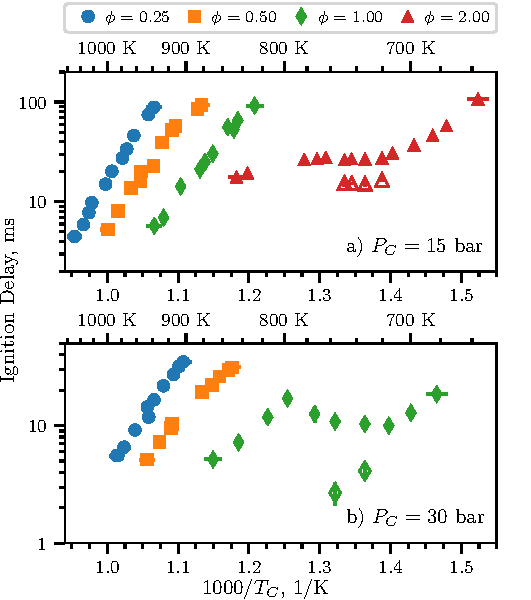
\includegraphics{figures/ignition-delays.pdf}
    \caption{Ignition delays of MV as a function of inverse temperature. Filled
    points are the overall ignition delays and hollow points are the first stage
    ignition delays. a) \SI{15}{\bar}. b) \SI{30}{\bar}}
    \label{fig:ignition-delays}
\end{center}

\citet{Hadj-Ali2009} also observed two-stage ignition of MV in stoichiometric mixtures, stating that
``[m]ethyl pentanoate... was more reactive [than methyl butanoate] with a limit below which
autoignition no longer occurs observed at \(T_c = \SI{670}{\K}\) and \(P_c = \SI{11.4}{\bar}\). At
this temperature, the autoignition occurred in two stages with a clearly identified cool flame
event.''\cite{Hadj-Ali2009} However, we do not find two stage ignition for the similar pressure of
\(P_C = \SI{15}{\bar}\) in this study. We note that the stated temperature of the experiment from
the work of \citet{Hadj-Ali2009} (\SI{670}{\K}) is much lower than the lowest temperature we
considered in this work at \SI{15}{\bar}, \(\phi=1.0\) (\SI{828}{\K}). We did not conduct
experiments at lower temperatures because the work of \citet{Mittal2006} showed that the temperature
field in the RCM reaction chamber was uniform for approximately \SI{100}{\ms} after the EOC, and our
measured ignition delay at \SI{15}{\bar}, \(\phi=1.0\) \SI{828}{\K} is \SI{92.14}{\ms}.

However, we note NTC behavior of the ignition delay and two-stage ignition at the higher pressure of
\SI{30}{\bar}, and at higher temperatures than those reported for two-stage ignition in the study of
\citet{Hadj-Ali2009}. The trend of NTC behavior shifting to higher temperatures with increasing
pressure can be seen in other classes of fuels. \citet{Kukkadapu2012} found a similar trend in
gasoline composed of iso-alkanes, n-alkanes, cyclo-alkanes, aromatics, and olefins.
\citet{Kukkadapu2012} attributed the NTC shift to the reactions between the hydroperoxyalkyl radical
(\ce{QOOH}) and \ce{O2} becoming more dominant than the unimolecular decomposition of \ce{QOOH} at
higher pressures. Similar trends could occur for the hydroperoxyalkyl radicals of MV.

To further understand the effect of the methyl ester functional group on the NTC region of ignition
delay, we compare with the alkane and alcohol with 5-carbon alkyl chains, n-pentane and n-pentanol.
n-Pentane and MV have the same fuel mole percentage for stoichiometric mixtures in air
(\SI{2.56}{\percent}), while n-pentanol has a fuel mole percentage of \SI{2.72}{\percent} for
stoichiometric conditions. \citet{Ribaucour1998} and \citet{Bugler2015} found the NTC region for
n-pentane to be between \SIlist{760;910}{\K} at pressures near \SI{10}{\atm}. As we will compare
with our MV data at \SI{30}{\bar}, we note that increasing the pressure tends to shift the NTC
to higher temperatures, as mentioned previously \cite{Kukkadapu2012}. \citet{Heufer2013} found NTC
behavior for n-pentanol in the range of \SIrange{770}{900}{\K} at \SI{30}{\bar}. In this study, we
find the NTC window for MV at \SI{30}{\bar} to be between \SIlist{720;800}{\K}. Therefore, it
appears that the methyl ester functional group shifts the NTC range to lower temperature as compared
to alkanes and alcohols with similar alkyl chain lengths. This result was also noted by
\citet{Hadj-Ali2009} for MHEX as the fuel.

\subsection{Pressure Traces}\label{sec:pressure-traces}

\Cref{fig:pressure-traces}a shows the pressure traces for selected experiments at \(\phi=1.0\),
\(P_C =\SI[number-unit-product={\ }]{30}{\bar}\). The three reactive pressure traces shown are at
the low-temperature end of the NTC (blue, \SI{700}{\K}), one case with two-stage ignition (orange,
\SI{733}{\K}), and one case near the high-temperature limit of the NTC region (green, \SI{774}{\K}).
Also shown is the non-reactive pressure trace for the \SI{700}{\K} case (red). By comparing the
\SI{700}{\K} pressure trace with the non-reactive pressure trace, it can be seen that there is
substantial heat release prior to main ignition as measured by the deviation of the reactive
pressure trace from the non-reactive trace. However, there is only one peak in the time derivative
of the pressure, so no first-stage ignition delay is defined for this case. It can also be seen in
\cref{fig:pressure-traces}a that the \SI{775}{\K} case shows some heat release prior to ignition,
although again there is only one peak in the time derivative of the pressure. Furthermore, the heat
release at \SI{775}{\K} appears to be more gradual than at the lowest temperature.

\begin{center}
    \captionsetup{type=figure}
    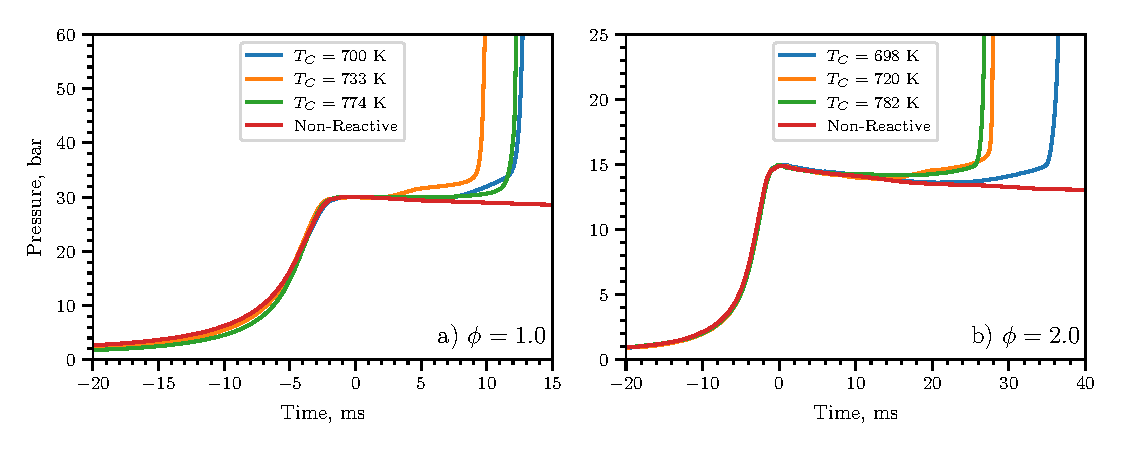
\includegraphics[width=\textwidth]{figures/pressure-traces.pdf}
    \caption{Selected pressure traces around the NTC region of ignition delay.
    a) \(\phi=1.0\) b) \(\phi=2.0\)}
    \label{fig:pressure-traces}
\end{center}

A similar trend can be observed in \cref{fig:pressure-traces}b for \(\phi=2.0\) at
\(P_C=\SI{15}{\bar}\), where pressure traces at several points around the NTC region are plotted. As
in \cref{fig:pressure-traces}a, the three reactive pressure traces shown are at the low-temperature
end of the NTC (blue, \SI{698}{\K}), one case with two-stage ignition (orange, \SI{720}{\K}), and
one case near the high-temperature limit of the NTC region (green, \SI{782}{\K}). Also shown is the
non-reactive pressure trace for the \SI{698}{\K} case (red). As for the \(\phi=1.0\) case, the
pressure traces show significant heat release prior to the overall ignition, as judged by deviation
from the non-reactive case.

\section{Computational Results}\label{sec:computational-results}

\Cref{fig:simulation-comparison} compares experimentally measured overall ignition delays with
ignition delays computed with the detailed model of \citet{Dievart2013} (solid lines).
\Cref{fig:simulation-comparison}a shows results at \(P_C = \SI{15}{\bar}\), while
\cref{fig:simulation-comparison}b shows results at \(P_C = \SI{30}{\bar}\). Only some equivalence
ratios are shown for each pressure condition; data and simulated results are not shown for cases
where the reactive simulated temperature at the EOC deviated substantially from the non-reactive
temperature due to heat release during the compression stroke. Furthermore, it is important to note
that the model of \citet{Dievart2013} was not validated for MV ignition delays, only for extinction
strain rates.

\begin{center}
    \captionsetup{type=figure}
    \resizebox{\textwidth}{!}{%% Creator: Matplotlib, PGF backend
%%
%% To include the figure in your LaTeX document, write
%%   \input{<filename>.pgf}
%%
%% Make sure the required packages are loaded in your preamble
%%   \usepackage{pgf}
%%
%% Figures using additional raster images can only be included by \input if
%% they are in the same directory as the main LaTeX file. For loading figures
%% from other directories you can use the `import` package
%%   \usepackage{import}
%% and then include the figures with
%%   \import{<path to file>}{<filename>.pgf}
%%
%% Matplotlib used the following preamble
%%   \usepackage{mathtools}
%%
\begingroup%
\makeatletter%
\begin{pgfpicture}%
\pgfpathrectangle{\pgfpointorigin}{\pgfqpoint{7.480315in}{3.000000in}}%
\pgfusepath{use as bounding box, clip}%
\begin{pgfscope}%
\pgfsetbuttcap%
\pgfsetmiterjoin%
\definecolor{currentfill}{rgb}{1.000000,1.000000,1.000000}%
\pgfsetfillcolor{currentfill}%
\pgfsetlinewidth{0.000000pt}%
\definecolor{currentstroke}{rgb}{1.000000,1.000000,1.000000}%
\pgfsetstrokecolor{currentstroke}%
\pgfsetdash{}{0pt}%
\pgfpathmoveto{\pgfqpoint{0.000000in}{0.000000in}}%
\pgfpathlineto{\pgfqpoint{7.480315in}{0.000000in}}%
\pgfpathlineto{\pgfqpoint{7.480315in}{3.000000in}}%
\pgfpathlineto{\pgfqpoint{0.000000in}{3.000000in}}%
\pgfpathclose%
\pgfusepath{fill}%
\end{pgfscope}%
\begin{pgfscope}%
\pgfsetbuttcap%
\pgfsetmiterjoin%
\definecolor{currentfill}{rgb}{1.000000,1.000000,1.000000}%
\pgfsetfillcolor{currentfill}%
\pgfsetlinewidth{0.000000pt}%
\definecolor{currentstroke}{rgb}{0.000000,0.000000,0.000000}%
\pgfsetstrokecolor{currentstroke}%
\pgfsetstrokeopacity{0.000000}%
\pgfsetdash{}{0pt}%
\pgfpathmoveto{\pgfqpoint{0.490763in}{0.409167in}}%
\pgfpathlineto{\pgfqpoint{3.600157in}{0.409167in}}%
\pgfpathlineto{\pgfqpoint{3.600157in}{2.520000in}}%
\pgfpathlineto{\pgfqpoint{0.490763in}{2.520000in}}%
\pgfpathclose%
\pgfusepath{fill}%
\end{pgfscope}%
\begin{pgfscope}%
\pgfsetbuttcap%
\pgfsetroundjoin%
\definecolor{currentfill}{rgb}{0.000000,0.000000,0.000000}%
\pgfsetfillcolor{currentfill}%
\pgfsetlinewidth{1.003750pt}%
\definecolor{currentstroke}{rgb}{0.000000,0.000000,0.000000}%
\pgfsetstrokecolor{currentstroke}%
\pgfsetdash{}{0pt}%
\pgfsys@defobject{currentmarker}{\pgfqpoint{0.000000in}{-0.069444in}}{\pgfqpoint{0.000000in}{0.000000in}}{%
\pgfpathmoveto{\pgfqpoint{0.000000in}{0.000000in}}%
\pgfpathlineto{\pgfqpoint{0.000000in}{-0.069444in}}%
\pgfusepath{stroke,fill}%
}%
\begin{pgfscope}%
\pgfsys@transformshift{0.796605in}{0.409167in}%
\pgfsys@useobject{currentmarker}{}%
\end{pgfscope}%
\end{pgfscope}%
\begin{pgfscope}%
\pgftext[x=0.796605in,y=0.291111in,,top]{\rmfamily\fontsize{9.000000}{10.800000}\selectfont \(\displaystyle 1.0\)}%
\end{pgfscope}%
\begin{pgfscope}%
\pgfsetbuttcap%
\pgfsetroundjoin%
\definecolor{currentfill}{rgb}{0.000000,0.000000,0.000000}%
\pgfsetfillcolor{currentfill}%
\pgfsetlinewidth{1.003750pt}%
\definecolor{currentstroke}{rgb}{0.000000,0.000000,0.000000}%
\pgfsetstrokecolor{currentstroke}%
\pgfsetdash{}{0pt}%
\pgfsys@defobject{currentmarker}{\pgfqpoint{0.000000in}{-0.069444in}}{\pgfqpoint{0.000000in}{0.000000in}}{%
\pgfpathmoveto{\pgfqpoint{0.000000in}{0.000000in}}%
\pgfpathlineto{\pgfqpoint{0.000000in}{-0.069444in}}%
\pgfusepath{stroke,fill}%
}%
\begin{pgfscope}%
\pgfsys@transformshift{1.306342in}{0.409167in}%
\pgfsys@useobject{currentmarker}{}%
\end{pgfscope}%
\end{pgfscope}%
\begin{pgfscope}%
\pgftext[x=1.306342in,y=0.291111in,,top]{\rmfamily\fontsize{9.000000}{10.800000}\selectfont \(\displaystyle 1.1\)}%
\end{pgfscope}%
\begin{pgfscope}%
\pgfsetbuttcap%
\pgfsetroundjoin%
\definecolor{currentfill}{rgb}{0.000000,0.000000,0.000000}%
\pgfsetfillcolor{currentfill}%
\pgfsetlinewidth{1.003750pt}%
\definecolor{currentstroke}{rgb}{0.000000,0.000000,0.000000}%
\pgfsetstrokecolor{currentstroke}%
\pgfsetdash{}{0pt}%
\pgfsys@defobject{currentmarker}{\pgfqpoint{0.000000in}{-0.069444in}}{\pgfqpoint{0.000000in}{0.000000in}}{%
\pgfpathmoveto{\pgfqpoint{0.000000in}{0.000000in}}%
\pgfpathlineto{\pgfqpoint{0.000000in}{-0.069444in}}%
\pgfusepath{stroke,fill}%
}%
\begin{pgfscope}%
\pgfsys@transformshift{1.816078in}{0.409167in}%
\pgfsys@useobject{currentmarker}{}%
\end{pgfscope}%
\end{pgfscope}%
\begin{pgfscope}%
\pgftext[x=1.816078in,y=0.291111in,,top]{\rmfamily\fontsize{9.000000}{10.800000}\selectfont \(\displaystyle 1.2\)}%
\end{pgfscope}%
\begin{pgfscope}%
\pgfsetbuttcap%
\pgfsetroundjoin%
\definecolor{currentfill}{rgb}{0.000000,0.000000,0.000000}%
\pgfsetfillcolor{currentfill}%
\pgfsetlinewidth{1.003750pt}%
\definecolor{currentstroke}{rgb}{0.000000,0.000000,0.000000}%
\pgfsetstrokecolor{currentstroke}%
\pgfsetdash{}{0pt}%
\pgfsys@defobject{currentmarker}{\pgfqpoint{0.000000in}{-0.069444in}}{\pgfqpoint{0.000000in}{0.000000in}}{%
\pgfpathmoveto{\pgfqpoint{0.000000in}{0.000000in}}%
\pgfpathlineto{\pgfqpoint{0.000000in}{-0.069444in}}%
\pgfusepath{stroke,fill}%
}%
\begin{pgfscope}%
\pgfsys@transformshift{2.325815in}{0.409167in}%
\pgfsys@useobject{currentmarker}{}%
\end{pgfscope}%
\end{pgfscope}%
\begin{pgfscope}%
\pgftext[x=2.325815in,y=0.291111in,,top]{\rmfamily\fontsize{9.000000}{10.800000}\selectfont \(\displaystyle 1.3\)}%
\end{pgfscope}%
\begin{pgfscope}%
\pgfsetbuttcap%
\pgfsetroundjoin%
\definecolor{currentfill}{rgb}{0.000000,0.000000,0.000000}%
\pgfsetfillcolor{currentfill}%
\pgfsetlinewidth{1.003750pt}%
\definecolor{currentstroke}{rgb}{0.000000,0.000000,0.000000}%
\pgfsetstrokecolor{currentstroke}%
\pgfsetdash{}{0pt}%
\pgfsys@defobject{currentmarker}{\pgfqpoint{0.000000in}{-0.069444in}}{\pgfqpoint{0.000000in}{0.000000in}}{%
\pgfpathmoveto{\pgfqpoint{0.000000in}{0.000000in}}%
\pgfpathlineto{\pgfqpoint{0.000000in}{-0.069444in}}%
\pgfusepath{stroke,fill}%
}%
\begin{pgfscope}%
\pgfsys@transformshift{2.835552in}{0.409167in}%
\pgfsys@useobject{currentmarker}{}%
\end{pgfscope}%
\end{pgfscope}%
\begin{pgfscope}%
\pgftext[x=2.835552in,y=0.291111in,,top]{\rmfamily\fontsize{9.000000}{10.800000}\selectfont \(\displaystyle 1.4\)}%
\end{pgfscope}%
\begin{pgfscope}%
\pgfsetbuttcap%
\pgfsetroundjoin%
\definecolor{currentfill}{rgb}{0.000000,0.000000,0.000000}%
\pgfsetfillcolor{currentfill}%
\pgfsetlinewidth{1.003750pt}%
\definecolor{currentstroke}{rgb}{0.000000,0.000000,0.000000}%
\pgfsetstrokecolor{currentstroke}%
\pgfsetdash{}{0pt}%
\pgfsys@defobject{currentmarker}{\pgfqpoint{0.000000in}{-0.069444in}}{\pgfqpoint{0.000000in}{0.000000in}}{%
\pgfpathmoveto{\pgfqpoint{0.000000in}{0.000000in}}%
\pgfpathlineto{\pgfqpoint{0.000000in}{-0.069444in}}%
\pgfusepath{stroke,fill}%
}%
\begin{pgfscope}%
\pgfsys@transformshift{3.345289in}{0.409167in}%
\pgfsys@useobject{currentmarker}{}%
\end{pgfscope}%
\end{pgfscope}%
\begin{pgfscope}%
\pgftext[x=3.345289in,y=0.291111in,,top]{\rmfamily\fontsize{9.000000}{10.800000}\selectfont \(\displaystyle 1.5\)}%
\end{pgfscope}%
\begin{pgfscope}%
\pgfsetbuttcap%
\pgfsetroundjoin%
\definecolor{currentfill}{rgb}{0.000000,0.000000,0.000000}%
\pgfsetfillcolor{currentfill}%
\pgfsetlinewidth{1.003750pt}%
\definecolor{currentstroke}{rgb}{0.000000,0.000000,0.000000}%
\pgfsetstrokecolor{currentstroke}%
\pgfsetdash{}{0pt}%
\pgfsys@defobject{currentmarker}{\pgfqpoint{0.000000in}{-0.034722in}}{\pgfqpoint{0.000000in}{0.000000in}}{%
\pgfpathmoveto{\pgfqpoint{0.000000in}{0.000000in}}%
\pgfpathlineto{\pgfqpoint{0.000000in}{-0.034722in}}%
\pgfusepath{stroke,fill}%
}%
\begin{pgfscope}%
\pgfsys@transformshift{0.541736in}{0.409167in}%
\pgfsys@useobject{currentmarker}{}%
\end{pgfscope}%
\end{pgfscope}%
\begin{pgfscope}%
\pgfsetbuttcap%
\pgfsetroundjoin%
\definecolor{currentfill}{rgb}{0.000000,0.000000,0.000000}%
\pgfsetfillcolor{currentfill}%
\pgfsetlinewidth{1.003750pt}%
\definecolor{currentstroke}{rgb}{0.000000,0.000000,0.000000}%
\pgfsetstrokecolor{currentstroke}%
\pgfsetdash{}{0pt}%
\pgfsys@defobject{currentmarker}{\pgfqpoint{0.000000in}{-0.034722in}}{\pgfqpoint{0.000000in}{0.000000in}}{%
\pgfpathmoveto{\pgfqpoint{0.000000in}{0.000000in}}%
\pgfpathlineto{\pgfqpoint{0.000000in}{-0.034722in}}%
\pgfusepath{stroke,fill}%
}%
\begin{pgfscope}%
\pgfsys@transformshift{0.669171in}{0.409167in}%
\pgfsys@useobject{currentmarker}{}%
\end{pgfscope}%
\end{pgfscope}%
\begin{pgfscope}%
\pgfsetbuttcap%
\pgfsetroundjoin%
\definecolor{currentfill}{rgb}{0.000000,0.000000,0.000000}%
\pgfsetfillcolor{currentfill}%
\pgfsetlinewidth{1.003750pt}%
\definecolor{currentstroke}{rgb}{0.000000,0.000000,0.000000}%
\pgfsetstrokecolor{currentstroke}%
\pgfsetdash{}{0pt}%
\pgfsys@defobject{currentmarker}{\pgfqpoint{0.000000in}{-0.034722in}}{\pgfqpoint{0.000000in}{0.000000in}}{%
\pgfpathmoveto{\pgfqpoint{0.000000in}{0.000000in}}%
\pgfpathlineto{\pgfqpoint{0.000000in}{-0.034722in}}%
\pgfusepath{stroke,fill}%
}%
\begin{pgfscope}%
\pgfsys@transformshift{0.924039in}{0.409167in}%
\pgfsys@useobject{currentmarker}{}%
\end{pgfscope}%
\end{pgfscope}%
\begin{pgfscope}%
\pgfsetbuttcap%
\pgfsetroundjoin%
\definecolor{currentfill}{rgb}{0.000000,0.000000,0.000000}%
\pgfsetfillcolor{currentfill}%
\pgfsetlinewidth{1.003750pt}%
\definecolor{currentstroke}{rgb}{0.000000,0.000000,0.000000}%
\pgfsetstrokecolor{currentstroke}%
\pgfsetdash{}{0pt}%
\pgfsys@defobject{currentmarker}{\pgfqpoint{0.000000in}{-0.034722in}}{\pgfqpoint{0.000000in}{0.000000in}}{%
\pgfpathmoveto{\pgfqpoint{0.000000in}{0.000000in}}%
\pgfpathlineto{\pgfqpoint{0.000000in}{-0.034722in}}%
\pgfusepath{stroke,fill}%
}%
\begin{pgfscope}%
\pgfsys@transformshift{1.051473in}{0.409167in}%
\pgfsys@useobject{currentmarker}{}%
\end{pgfscope}%
\end{pgfscope}%
\begin{pgfscope}%
\pgfsetbuttcap%
\pgfsetroundjoin%
\definecolor{currentfill}{rgb}{0.000000,0.000000,0.000000}%
\pgfsetfillcolor{currentfill}%
\pgfsetlinewidth{1.003750pt}%
\definecolor{currentstroke}{rgb}{0.000000,0.000000,0.000000}%
\pgfsetstrokecolor{currentstroke}%
\pgfsetdash{}{0pt}%
\pgfsys@defobject{currentmarker}{\pgfqpoint{0.000000in}{-0.034722in}}{\pgfqpoint{0.000000in}{0.000000in}}{%
\pgfpathmoveto{\pgfqpoint{0.000000in}{0.000000in}}%
\pgfpathlineto{\pgfqpoint{0.000000in}{-0.034722in}}%
\pgfusepath{stroke,fill}%
}%
\begin{pgfscope}%
\pgfsys@transformshift{1.178907in}{0.409167in}%
\pgfsys@useobject{currentmarker}{}%
\end{pgfscope}%
\end{pgfscope}%
\begin{pgfscope}%
\pgfsetbuttcap%
\pgfsetroundjoin%
\definecolor{currentfill}{rgb}{0.000000,0.000000,0.000000}%
\pgfsetfillcolor{currentfill}%
\pgfsetlinewidth{1.003750pt}%
\definecolor{currentstroke}{rgb}{0.000000,0.000000,0.000000}%
\pgfsetstrokecolor{currentstroke}%
\pgfsetdash{}{0pt}%
\pgfsys@defobject{currentmarker}{\pgfqpoint{0.000000in}{-0.034722in}}{\pgfqpoint{0.000000in}{0.000000in}}{%
\pgfpathmoveto{\pgfqpoint{0.000000in}{0.000000in}}%
\pgfpathlineto{\pgfqpoint{0.000000in}{-0.034722in}}%
\pgfusepath{stroke,fill}%
}%
\begin{pgfscope}%
\pgfsys@transformshift{1.433776in}{0.409167in}%
\pgfsys@useobject{currentmarker}{}%
\end{pgfscope}%
\end{pgfscope}%
\begin{pgfscope}%
\pgfsetbuttcap%
\pgfsetroundjoin%
\definecolor{currentfill}{rgb}{0.000000,0.000000,0.000000}%
\pgfsetfillcolor{currentfill}%
\pgfsetlinewidth{1.003750pt}%
\definecolor{currentstroke}{rgb}{0.000000,0.000000,0.000000}%
\pgfsetstrokecolor{currentstroke}%
\pgfsetdash{}{0pt}%
\pgfsys@defobject{currentmarker}{\pgfqpoint{0.000000in}{-0.034722in}}{\pgfqpoint{0.000000in}{0.000000in}}{%
\pgfpathmoveto{\pgfqpoint{0.000000in}{0.000000in}}%
\pgfpathlineto{\pgfqpoint{0.000000in}{-0.034722in}}%
\pgfusepath{stroke,fill}%
}%
\begin{pgfscope}%
\pgfsys@transformshift{1.561210in}{0.409167in}%
\pgfsys@useobject{currentmarker}{}%
\end{pgfscope}%
\end{pgfscope}%
\begin{pgfscope}%
\pgfsetbuttcap%
\pgfsetroundjoin%
\definecolor{currentfill}{rgb}{0.000000,0.000000,0.000000}%
\pgfsetfillcolor{currentfill}%
\pgfsetlinewidth{1.003750pt}%
\definecolor{currentstroke}{rgb}{0.000000,0.000000,0.000000}%
\pgfsetstrokecolor{currentstroke}%
\pgfsetdash{}{0pt}%
\pgfsys@defobject{currentmarker}{\pgfqpoint{0.000000in}{-0.034722in}}{\pgfqpoint{0.000000in}{0.000000in}}{%
\pgfpathmoveto{\pgfqpoint{0.000000in}{0.000000in}}%
\pgfpathlineto{\pgfqpoint{0.000000in}{-0.034722in}}%
\pgfusepath{stroke,fill}%
}%
\begin{pgfscope}%
\pgfsys@transformshift{1.688644in}{0.409167in}%
\pgfsys@useobject{currentmarker}{}%
\end{pgfscope}%
\end{pgfscope}%
\begin{pgfscope}%
\pgfsetbuttcap%
\pgfsetroundjoin%
\definecolor{currentfill}{rgb}{0.000000,0.000000,0.000000}%
\pgfsetfillcolor{currentfill}%
\pgfsetlinewidth{1.003750pt}%
\definecolor{currentstroke}{rgb}{0.000000,0.000000,0.000000}%
\pgfsetstrokecolor{currentstroke}%
\pgfsetdash{}{0pt}%
\pgfsys@defobject{currentmarker}{\pgfqpoint{0.000000in}{-0.034722in}}{\pgfqpoint{0.000000in}{0.000000in}}{%
\pgfpathmoveto{\pgfqpoint{0.000000in}{0.000000in}}%
\pgfpathlineto{\pgfqpoint{0.000000in}{-0.034722in}}%
\pgfusepath{stroke,fill}%
}%
\begin{pgfscope}%
\pgfsys@transformshift{1.943513in}{0.409167in}%
\pgfsys@useobject{currentmarker}{}%
\end{pgfscope}%
\end{pgfscope}%
\begin{pgfscope}%
\pgfsetbuttcap%
\pgfsetroundjoin%
\definecolor{currentfill}{rgb}{0.000000,0.000000,0.000000}%
\pgfsetfillcolor{currentfill}%
\pgfsetlinewidth{1.003750pt}%
\definecolor{currentstroke}{rgb}{0.000000,0.000000,0.000000}%
\pgfsetstrokecolor{currentstroke}%
\pgfsetdash{}{0pt}%
\pgfsys@defobject{currentmarker}{\pgfqpoint{0.000000in}{-0.034722in}}{\pgfqpoint{0.000000in}{0.000000in}}{%
\pgfpathmoveto{\pgfqpoint{0.000000in}{0.000000in}}%
\pgfpathlineto{\pgfqpoint{0.000000in}{-0.034722in}}%
\pgfusepath{stroke,fill}%
}%
\begin{pgfscope}%
\pgfsys@transformshift{2.070947in}{0.409167in}%
\pgfsys@useobject{currentmarker}{}%
\end{pgfscope}%
\end{pgfscope}%
\begin{pgfscope}%
\pgfsetbuttcap%
\pgfsetroundjoin%
\definecolor{currentfill}{rgb}{0.000000,0.000000,0.000000}%
\pgfsetfillcolor{currentfill}%
\pgfsetlinewidth{1.003750pt}%
\definecolor{currentstroke}{rgb}{0.000000,0.000000,0.000000}%
\pgfsetstrokecolor{currentstroke}%
\pgfsetdash{}{0pt}%
\pgfsys@defobject{currentmarker}{\pgfqpoint{0.000000in}{-0.034722in}}{\pgfqpoint{0.000000in}{0.000000in}}{%
\pgfpathmoveto{\pgfqpoint{0.000000in}{0.000000in}}%
\pgfpathlineto{\pgfqpoint{0.000000in}{-0.034722in}}%
\pgfusepath{stroke,fill}%
}%
\begin{pgfscope}%
\pgfsys@transformshift{2.198381in}{0.409167in}%
\pgfsys@useobject{currentmarker}{}%
\end{pgfscope}%
\end{pgfscope}%
\begin{pgfscope}%
\pgfsetbuttcap%
\pgfsetroundjoin%
\definecolor{currentfill}{rgb}{0.000000,0.000000,0.000000}%
\pgfsetfillcolor{currentfill}%
\pgfsetlinewidth{1.003750pt}%
\definecolor{currentstroke}{rgb}{0.000000,0.000000,0.000000}%
\pgfsetstrokecolor{currentstroke}%
\pgfsetdash{}{0pt}%
\pgfsys@defobject{currentmarker}{\pgfqpoint{0.000000in}{-0.034722in}}{\pgfqpoint{0.000000in}{0.000000in}}{%
\pgfpathmoveto{\pgfqpoint{0.000000in}{0.000000in}}%
\pgfpathlineto{\pgfqpoint{0.000000in}{-0.034722in}}%
\pgfusepath{stroke,fill}%
}%
\begin{pgfscope}%
\pgfsys@transformshift{2.325815in}{0.409167in}%
\pgfsys@useobject{currentmarker}{}%
\end{pgfscope}%
\end{pgfscope}%
\begin{pgfscope}%
\pgfsetbuttcap%
\pgfsetroundjoin%
\definecolor{currentfill}{rgb}{0.000000,0.000000,0.000000}%
\pgfsetfillcolor{currentfill}%
\pgfsetlinewidth{1.003750pt}%
\definecolor{currentstroke}{rgb}{0.000000,0.000000,0.000000}%
\pgfsetstrokecolor{currentstroke}%
\pgfsetdash{}{0pt}%
\pgfsys@defobject{currentmarker}{\pgfqpoint{0.000000in}{-0.034722in}}{\pgfqpoint{0.000000in}{0.000000in}}{%
\pgfpathmoveto{\pgfqpoint{0.000000in}{0.000000in}}%
\pgfpathlineto{\pgfqpoint{0.000000in}{-0.034722in}}%
\pgfusepath{stroke,fill}%
}%
\begin{pgfscope}%
\pgfsys@transformshift{2.453250in}{0.409167in}%
\pgfsys@useobject{currentmarker}{}%
\end{pgfscope}%
\end{pgfscope}%
\begin{pgfscope}%
\pgfsetbuttcap%
\pgfsetroundjoin%
\definecolor{currentfill}{rgb}{0.000000,0.000000,0.000000}%
\pgfsetfillcolor{currentfill}%
\pgfsetlinewidth{1.003750pt}%
\definecolor{currentstroke}{rgb}{0.000000,0.000000,0.000000}%
\pgfsetstrokecolor{currentstroke}%
\pgfsetdash{}{0pt}%
\pgfsys@defobject{currentmarker}{\pgfqpoint{0.000000in}{-0.034722in}}{\pgfqpoint{0.000000in}{0.000000in}}{%
\pgfpathmoveto{\pgfqpoint{0.000000in}{0.000000in}}%
\pgfpathlineto{\pgfqpoint{0.000000in}{-0.034722in}}%
\pgfusepath{stroke,fill}%
}%
\begin{pgfscope}%
\pgfsys@transformshift{2.580684in}{0.409167in}%
\pgfsys@useobject{currentmarker}{}%
\end{pgfscope}%
\end{pgfscope}%
\begin{pgfscope}%
\pgfsetbuttcap%
\pgfsetroundjoin%
\definecolor{currentfill}{rgb}{0.000000,0.000000,0.000000}%
\pgfsetfillcolor{currentfill}%
\pgfsetlinewidth{1.003750pt}%
\definecolor{currentstroke}{rgb}{0.000000,0.000000,0.000000}%
\pgfsetstrokecolor{currentstroke}%
\pgfsetdash{}{0pt}%
\pgfsys@defobject{currentmarker}{\pgfqpoint{0.000000in}{-0.034722in}}{\pgfqpoint{0.000000in}{0.000000in}}{%
\pgfpathmoveto{\pgfqpoint{0.000000in}{0.000000in}}%
\pgfpathlineto{\pgfqpoint{0.000000in}{-0.034722in}}%
\pgfusepath{stroke,fill}%
}%
\begin{pgfscope}%
\pgfsys@transformshift{2.708118in}{0.409167in}%
\pgfsys@useobject{currentmarker}{}%
\end{pgfscope}%
\end{pgfscope}%
\begin{pgfscope}%
\pgfsetbuttcap%
\pgfsetroundjoin%
\definecolor{currentfill}{rgb}{0.000000,0.000000,0.000000}%
\pgfsetfillcolor{currentfill}%
\pgfsetlinewidth{1.003750pt}%
\definecolor{currentstroke}{rgb}{0.000000,0.000000,0.000000}%
\pgfsetstrokecolor{currentstroke}%
\pgfsetdash{}{0pt}%
\pgfsys@defobject{currentmarker}{\pgfqpoint{0.000000in}{-0.034722in}}{\pgfqpoint{0.000000in}{0.000000in}}{%
\pgfpathmoveto{\pgfqpoint{0.000000in}{0.000000in}}%
\pgfpathlineto{\pgfqpoint{0.000000in}{-0.034722in}}%
\pgfusepath{stroke,fill}%
}%
\begin{pgfscope}%
\pgfsys@transformshift{2.962986in}{0.409167in}%
\pgfsys@useobject{currentmarker}{}%
\end{pgfscope}%
\end{pgfscope}%
\begin{pgfscope}%
\pgfsetbuttcap%
\pgfsetroundjoin%
\definecolor{currentfill}{rgb}{0.000000,0.000000,0.000000}%
\pgfsetfillcolor{currentfill}%
\pgfsetlinewidth{1.003750pt}%
\definecolor{currentstroke}{rgb}{0.000000,0.000000,0.000000}%
\pgfsetstrokecolor{currentstroke}%
\pgfsetdash{}{0pt}%
\pgfsys@defobject{currentmarker}{\pgfqpoint{0.000000in}{-0.034722in}}{\pgfqpoint{0.000000in}{0.000000in}}{%
\pgfpathmoveto{\pgfqpoint{0.000000in}{0.000000in}}%
\pgfpathlineto{\pgfqpoint{0.000000in}{-0.034722in}}%
\pgfusepath{stroke,fill}%
}%
\begin{pgfscope}%
\pgfsys@transformshift{3.090421in}{0.409167in}%
\pgfsys@useobject{currentmarker}{}%
\end{pgfscope}%
\end{pgfscope}%
\begin{pgfscope}%
\pgfsetbuttcap%
\pgfsetroundjoin%
\definecolor{currentfill}{rgb}{0.000000,0.000000,0.000000}%
\pgfsetfillcolor{currentfill}%
\pgfsetlinewidth{1.003750pt}%
\definecolor{currentstroke}{rgb}{0.000000,0.000000,0.000000}%
\pgfsetstrokecolor{currentstroke}%
\pgfsetdash{}{0pt}%
\pgfsys@defobject{currentmarker}{\pgfqpoint{0.000000in}{-0.034722in}}{\pgfqpoint{0.000000in}{0.000000in}}{%
\pgfpathmoveto{\pgfqpoint{0.000000in}{0.000000in}}%
\pgfpathlineto{\pgfqpoint{0.000000in}{-0.034722in}}%
\pgfusepath{stroke,fill}%
}%
\begin{pgfscope}%
\pgfsys@transformshift{3.217855in}{0.409167in}%
\pgfsys@useobject{currentmarker}{}%
\end{pgfscope}%
\end{pgfscope}%
\begin{pgfscope}%
\pgfsetbuttcap%
\pgfsetroundjoin%
\definecolor{currentfill}{rgb}{0.000000,0.000000,0.000000}%
\pgfsetfillcolor{currentfill}%
\pgfsetlinewidth{1.003750pt}%
\definecolor{currentstroke}{rgb}{0.000000,0.000000,0.000000}%
\pgfsetstrokecolor{currentstroke}%
\pgfsetdash{}{0pt}%
\pgfsys@defobject{currentmarker}{\pgfqpoint{0.000000in}{-0.034722in}}{\pgfqpoint{0.000000in}{0.000000in}}{%
\pgfpathmoveto{\pgfqpoint{0.000000in}{0.000000in}}%
\pgfpathlineto{\pgfqpoint{0.000000in}{-0.034722in}}%
\pgfusepath{stroke,fill}%
}%
\begin{pgfscope}%
\pgfsys@transformshift{3.472723in}{0.409167in}%
\pgfsys@useobject{currentmarker}{}%
\end{pgfscope}%
\end{pgfscope}%
\begin{pgfscope}%
\pgfsetbuttcap%
\pgfsetroundjoin%
\definecolor{currentfill}{rgb}{0.000000,0.000000,0.000000}%
\pgfsetfillcolor{currentfill}%
\pgfsetlinewidth{1.003750pt}%
\definecolor{currentstroke}{rgb}{0.000000,0.000000,0.000000}%
\pgfsetstrokecolor{currentstroke}%
\pgfsetdash{}{0pt}%
\pgfsys@defobject{currentmarker}{\pgfqpoint{0.000000in}{-0.034722in}}{\pgfqpoint{0.000000in}{0.000000in}}{%
\pgfpathmoveto{\pgfqpoint{0.000000in}{0.000000in}}%
\pgfpathlineto{\pgfqpoint{0.000000in}{-0.034722in}}%
\pgfusepath{stroke,fill}%
}%
\begin{pgfscope}%
\pgfsys@transformshift{3.600157in}{0.409167in}%
\pgfsys@useobject{currentmarker}{}%
\end{pgfscope}%
\end{pgfscope}%
\begin{pgfscope}%
\pgfsetbuttcap%
\pgfsetroundjoin%
\definecolor{currentfill}{rgb}{0.000000,0.000000,0.000000}%
\pgfsetfillcolor{currentfill}%
\pgfsetlinewidth{1.003750pt}%
\definecolor{currentstroke}{rgb}{0.000000,0.000000,0.000000}%
\pgfsetstrokecolor{currentstroke}%
\pgfsetdash{}{0pt}%
\pgfsys@defobject{currentmarker}{\pgfqpoint{-0.069444in}{0.000000in}}{\pgfqpoint{0.000000in}{0.000000in}}{%
\pgfpathmoveto{\pgfqpoint{0.000000in}{0.000000in}}%
\pgfpathlineto{\pgfqpoint{-0.069444in}{0.000000in}}%
\pgfusepath{stroke,fill}%
}%
\begin{pgfscope}%
\pgfsys@transformshift{0.490763in}{0.409167in}%
\pgfsys@useobject{currentmarker}{}%
\end{pgfscope}%
\end{pgfscope}%
\begin{pgfscope}%
\pgftext[x=0.308471in,y=0.365764in,left,base]{\rmfamily\fontsize{9.000000}{10.800000}\selectfont 1}%
\end{pgfscope}%
\begin{pgfscope}%
\pgfsetbuttcap%
\pgfsetroundjoin%
\definecolor{currentfill}{rgb}{0.000000,0.000000,0.000000}%
\pgfsetfillcolor{currentfill}%
\pgfsetlinewidth{1.003750pt}%
\definecolor{currentstroke}{rgb}{0.000000,0.000000,0.000000}%
\pgfsetstrokecolor{currentstroke}%
\pgfsetdash{}{0pt}%
\pgfsys@defobject{currentmarker}{\pgfqpoint{-0.069444in}{0.000000in}}{\pgfqpoint{0.000000in}{0.000000in}}{%
\pgfpathmoveto{\pgfqpoint{0.000000in}{0.000000in}}%
\pgfpathlineto{\pgfqpoint{-0.069444in}{0.000000in}}%
\pgfusepath{stroke,fill}%
}%
\begin{pgfscope}%
\pgfsys@transformshift{0.490763in}{1.326509in}%
\pgfsys@useobject{currentmarker}{}%
\end{pgfscope}%
\end{pgfscope}%
\begin{pgfscope}%
\pgftext[x=0.244236in,y=1.283107in,left,base]{\rmfamily\fontsize{9.000000}{10.800000}\selectfont 10}%
\end{pgfscope}%
\begin{pgfscope}%
\pgfsetbuttcap%
\pgfsetroundjoin%
\definecolor{currentfill}{rgb}{0.000000,0.000000,0.000000}%
\pgfsetfillcolor{currentfill}%
\pgfsetlinewidth{1.003750pt}%
\definecolor{currentstroke}{rgb}{0.000000,0.000000,0.000000}%
\pgfsetstrokecolor{currentstroke}%
\pgfsetdash{}{0pt}%
\pgfsys@defobject{currentmarker}{\pgfqpoint{-0.069444in}{0.000000in}}{\pgfqpoint{0.000000in}{0.000000in}}{%
\pgfpathmoveto{\pgfqpoint{0.000000in}{0.000000in}}%
\pgfpathlineto{\pgfqpoint{-0.069444in}{0.000000in}}%
\pgfusepath{stroke,fill}%
}%
\begin{pgfscope}%
\pgfsys@transformshift{0.490763in}{2.243852in}%
\pgfsys@useobject{currentmarker}{}%
\end{pgfscope}%
\end{pgfscope}%
\begin{pgfscope}%
\pgftext[x=0.180000in,y=2.200450in,left,base]{\rmfamily\fontsize{9.000000}{10.800000}\selectfont 100}%
\end{pgfscope}%
\begin{pgfscope}%
\pgfsetbuttcap%
\pgfsetroundjoin%
\definecolor{currentfill}{rgb}{0.000000,0.000000,0.000000}%
\pgfsetfillcolor{currentfill}%
\pgfsetlinewidth{1.003750pt}%
\definecolor{currentstroke}{rgb}{0.000000,0.000000,0.000000}%
\pgfsetstrokecolor{currentstroke}%
\pgfsetdash{}{0pt}%
\pgfsys@defobject{currentmarker}{\pgfqpoint{-0.034722in}{0.000000in}}{\pgfqpoint{0.000000in}{0.000000in}}{%
\pgfpathmoveto{\pgfqpoint{0.000000in}{0.000000in}}%
\pgfpathlineto{\pgfqpoint{-0.034722in}{0.000000in}}%
\pgfusepath{stroke,fill}%
}%
\begin{pgfscope}%
\pgfsys@transformshift{0.490763in}{0.685314in}%
\pgfsys@useobject{currentmarker}{}%
\end{pgfscope}%
\end{pgfscope}%
\begin{pgfscope}%
\pgfsetbuttcap%
\pgfsetroundjoin%
\definecolor{currentfill}{rgb}{0.000000,0.000000,0.000000}%
\pgfsetfillcolor{currentfill}%
\pgfsetlinewidth{1.003750pt}%
\definecolor{currentstroke}{rgb}{0.000000,0.000000,0.000000}%
\pgfsetstrokecolor{currentstroke}%
\pgfsetdash{}{0pt}%
\pgfsys@defobject{currentmarker}{\pgfqpoint{-0.034722in}{0.000000in}}{\pgfqpoint{0.000000in}{0.000000in}}{%
\pgfpathmoveto{\pgfqpoint{0.000000in}{0.000000in}}%
\pgfpathlineto{\pgfqpoint{-0.034722in}{0.000000in}}%
\pgfusepath{stroke,fill}%
}%
\begin{pgfscope}%
\pgfsys@transformshift{0.490763in}{0.846850in}%
\pgfsys@useobject{currentmarker}{}%
\end{pgfscope}%
\end{pgfscope}%
\begin{pgfscope}%
\pgfsetbuttcap%
\pgfsetroundjoin%
\definecolor{currentfill}{rgb}{0.000000,0.000000,0.000000}%
\pgfsetfillcolor{currentfill}%
\pgfsetlinewidth{1.003750pt}%
\definecolor{currentstroke}{rgb}{0.000000,0.000000,0.000000}%
\pgfsetstrokecolor{currentstroke}%
\pgfsetdash{}{0pt}%
\pgfsys@defobject{currentmarker}{\pgfqpoint{-0.034722in}{0.000000in}}{\pgfqpoint{0.000000in}{0.000000in}}{%
\pgfpathmoveto{\pgfqpoint{0.000000in}{0.000000in}}%
\pgfpathlineto{\pgfqpoint{-0.034722in}{0.000000in}}%
\pgfusepath{stroke,fill}%
}%
\begin{pgfscope}%
\pgfsys@transformshift{0.490763in}{0.961462in}%
\pgfsys@useobject{currentmarker}{}%
\end{pgfscope}%
\end{pgfscope}%
\begin{pgfscope}%
\pgfsetbuttcap%
\pgfsetroundjoin%
\definecolor{currentfill}{rgb}{0.000000,0.000000,0.000000}%
\pgfsetfillcolor{currentfill}%
\pgfsetlinewidth{1.003750pt}%
\definecolor{currentstroke}{rgb}{0.000000,0.000000,0.000000}%
\pgfsetstrokecolor{currentstroke}%
\pgfsetdash{}{0pt}%
\pgfsys@defobject{currentmarker}{\pgfqpoint{-0.034722in}{0.000000in}}{\pgfqpoint{0.000000in}{0.000000in}}{%
\pgfpathmoveto{\pgfqpoint{0.000000in}{0.000000in}}%
\pgfpathlineto{\pgfqpoint{-0.034722in}{0.000000in}}%
\pgfusepath{stroke,fill}%
}%
\begin{pgfscope}%
\pgfsys@transformshift{0.490763in}{1.050362in}%
\pgfsys@useobject{currentmarker}{}%
\end{pgfscope}%
\end{pgfscope}%
\begin{pgfscope}%
\pgfsetbuttcap%
\pgfsetroundjoin%
\definecolor{currentfill}{rgb}{0.000000,0.000000,0.000000}%
\pgfsetfillcolor{currentfill}%
\pgfsetlinewidth{1.003750pt}%
\definecolor{currentstroke}{rgb}{0.000000,0.000000,0.000000}%
\pgfsetstrokecolor{currentstroke}%
\pgfsetdash{}{0pt}%
\pgfsys@defobject{currentmarker}{\pgfqpoint{-0.034722in}{0.000000in}}{\pgfqpoint{0.000000in}{0.000000in}}{%
\pgfpathmoveto{\pgfqpoint{0.000000in}{0.000000in}}%
\pgfpathlineto{\pgfqpoint{-0.034722in}{0.000000in}}%
\pgfusepath{stroke,fill}%
}%
\begin{pgfscope}%
\pgfsys@transformshift{0.490763in}{1.122998in}%
\pgfsys@useobject{currentmarker}{}%
\end{pgfscope}%
\end{pgfscope}%
\begin{pgfscope}%
\pgfsetbuttcap%
\pgfsetroundjoin%
\definecolor{currentfill}{rgb}{0.000000,0.000000,0.000000}%
\pgfsetfillcolor{currentfill}%
\pgfsetlinewidth{1.003750pt}%
\definecolor{currentstroke}{rgb}{0.000000,0.000000,0.000000}%
\pgfsetstrokecolor{currentstroke}%
\pgfsetdash{}{0pt}%
\pgfsys@defobject{currentmarker}{\pgfqpoint{-0.034722in}{0.000000in}}{\pgfqpoint{0.000000in}{0.000000in}}{%
\pgfpathmoveto{\pgfqpoint{0.000000in}{0.000000in}}%
\pgfpathlineto{\pgfqpoint{-0.034722in}{0.000000in}}%
\pgfusepath{stroke,fill}%
}%
\begin{pgfscope}%
\pgfsys@transformshift{0.490763in}{1.184411in}%
\pgfsys@useobject{currentmarker}{}%
\end{pgfscope}%
\end{pgfscope}%
\begin{pgfscope}%
\pgfsetbuttcap%
\pgfsetroundjoin%
\definecolor{currentfill}{rgb}{0.000000,0.000000,0.000000}%
\pgfsetfillcolor{currentfill}%
\pgfsetlinewidth{1.003750pt}%
\definecolor{currentstroke}{rgb}{0.000000,0.000000,0.000000}%
\pgfsetstrokecolor{currentstroke}%
\pgfsetdash{}{0pt}%
\pgfsys@defobject{currentmarker}{\pgfqpoint{-0.034722in}{0.000000in}}{\pgfqpoint{0.000000in}{0.000000in}}{%
\pgfpathmoveto{\pgfqpoint{0.000000in}{0.000000in}}%
\pgfpathlineto{\pgfqpoint{-0.034722in}{0.000000in}}%
\pgfusepath{stroke,fill}%
}%
\begin{pgfscope}%
\pgfsys@transformshift{0.490763in}{1.237610in}%
\pgfsys@useobject{currentmarker}{}%
\end{pgfscope}%
\end{pgfscope}%
\begin{pgfscope}%
\pgfsetbuttcap%
\pgfsetroundjoin%
\definecolor{currentfill}{rgb}{0.000000,0.000000,0.000000}%
\pgfsetfillcolor{currentfill}%
\pgfsetlinewidth{1.003750pt}%
\definecolor{currentstroke}{rgb}{0.000000,0.000000,0.000000}%
\pgfsetstrokecolor{currentstroke}%
\pgfsetdash{}{0pt}%
\pgfsys@defobject{currentmarker}{\pgfqpoint{-0.034722in}{0.000000in}}{\pgfqpoint{0.000000in}{0.000000in}}{%
\pgfpathmoveto{\pgfqpoint{0.000000in}{0.000000in}}%
\pgfpathlineto{\pgfqpoint{-0.034722in}{0.000000in}}%
\pgfusepath{stroke,fill}%
}%
\begin{pgfscope}%
\pgfsys@transformshift{0.490763in}{1.284534in}%
\pgfsys@useobject{currentmarker}{}%
\end{pgfscope}%
\end{pgfscope}%
\begin{pgfscope}%
\pgfsetbuttcap%
\pgfsetroundjoin%
\definecolor{currentfill}{rgb}{0.000000,0.000000,0.000000}%
\pgfsetfillcolor{currentfill}%
\pgfsetlinewidth{1.003750pt}%
\definecolor{currentstroke}{rgb}{0.000000,0.000000,0.000000}%
\pgfsetstrokecolor{currentstroke}%
\pgfsetdash{}{0pt}%
\pgfsys@defobject{currentmarker}{\pgfqpoint{-0.034722in}{0.000000in}}{\pgfqpoint{0.000000in}{0.000000in}}{%
\pgfpathmoveto{\pgfqpoint{0.000000in}{0.000000in}}%
\pgfpathlineto{\pgfqpoint{-0.034722in}{0.000000in}}%
\pgfusepath{stroke,fill}%
}%
\begin{pgfscope}%
\pgfsys@transformshift{0.490763in}{1.602657in}%
\pgfsys@useobject{currentmarker}{}%
\end{pgfscope}%
\end{pgfscope}%
\begin{pgfscope}%
\pgfsetbuttcap%
\pgfsetroundjoin%
\definecolor{currentfill}{rgb}{0.000000,0.000000,0.000000}%
\pgfsetfillcolor{currentfill}%
\pgfsetlinewidth{1.003750pt}%
\definecolor{currentstroke}{rgb}{0.000000,0.000000,0.000000}%
\pgfsetstrokecolor{currentstroke}%
\pgfsetdash{}{0pt}%
\pgfsys@defobject{currentmarker}{\pgfqpoint{-0.034722in}{0.000000in}}{\pgfqpoint{0.000000in}{0.000000in}}{%
\pgfpathmoveto{\pgfqpoint{0.000000in}{0.000000in}}%
\pgfpathlineto{\pgfqpoint{-0.034722in}{0.000000in}}%
\pgfusepath{stroke,fill}%
}%
\begin{pgfscope}%
\pgfsys@transformshift{0.490763in}{1.764193in}%
\pgfsys@useobject{currentmarker}{}%
\end{pgfscope}%
\end{pgfscope}%
\begin{pgfscope}%
\pgfsetbuttcap%
\pgfsetroundjoin%
\definecolor{currentfill}{rgb}{0.000000,0.000000,0.000000}%
\pgfsetfillcolor{currentfill}%
\pgfsetlinewidth{1.003750pt}%
\definecolor{currentstroke}{rgb}{0.000000,0.000000,0.000000}%
\pgfsetstrokecolor{currentstroke}%
\pgfsetdash{}{0pt}%
\pgfsys@defobject{currentmarker}{\pgfqpoint{-0.034722in}{0.000000in}}{\pgfqpoint{0.000000in}{0.000000in}}{%
\pgfpathmoveto{\pgfqpoint{0.000000in}{0.000000in}}%
\pgfpathlineto{\pgfqpoint{-0.034722in}{0.000000in}}%
\pgfusepath{stroke,fill}%
}%
\begin{pgfscope}%
\pgfsys@transformshift{0.490763in}{1.878805in}%
\pgfsys@useobject{currentmarker}{}%
\end{pgfscope}%
\end{pgfscope}%
\begin{pgfscope}%
\pgfsetbuttcap%
\pgfsetroundjoin%
\definecolor{currentfill}{rgb}{0.000000,0.000000,0.000000}%
\pgfsetfillcolor{currentfill}%
\pgfsetlinewidth{1.003750pt}%
\definecolor{currentstroke}{rgb}{0.000000,0.000000,0.000000}%
\pgfsetstrokecolor{currentstroke}%
\pgfsetdash{}{0pt}%
\pgfsys@defobject{currentmarker}{\pgfqpoint{-0.034722in}{0.000000in}}{\pgfqpoint{0.000000in}{0.000000in}}{%
\pgfpathmoveto{\pgfqpoint{0.000000in}{0.000000in}}%
\pgfpathlineto{\pgfqpoint{-0.034722in}{0.000000in}}%
\pgfusepath{stroke,fill}%
}%
\begin{pgfscope}%
\pgfsys@transformshift{0.490763in}{1.967705in}%
\pgfsys@useobject{currentmarker}{}%
\end{pgfscope}%
\end{pgfscope}%
\begin{pgfscope}%
\pgfsetbuttcap%
\pgfsetroundjoin%
\definecolor{currentfill}{rgb}{0.000000,0.000000,0.000000}%
\pgfsetfillcolor{currentfill}%
\pgfsetlinewidth{1.003750pt}%
\definecolor{currentstroke}{rgb}{0.000000,0.000000,0.000000}%
\pgfsetstrokecolor{currentstroke}%
\pgfsetdash{}{0pt}%
\pgfsys@defobject{currentmarker}{\pgfqpoint{-0.034722in}{0.000000in}}{\pgfqpoint{0.000000in}{0.000000in}}{%
\pgfpathmoveto{\pgfqpoint{0.000000in}{0.000000in}}%
\pgfpathlineto{\pgfqpoint{-0.034722in}{0.000000in}}%
\pgfusepath{stroke,fill}%
}%
\begin{pgfscope}%
\pgfsys@transformshift{0.490763in}{2.040341in}%
\pgfsys@useobject{currentmarker}{}%
\end{pgfscope}%
\end{pgfscope}%
\begin{pgfscope}%
\pgfsetbuttcap%
\pgfsetroundjoin%
\definecolor{currentfill}{rgb}{0.000000,0.000000,0.000000}%
\pgfsetfillcolor{currentfill}%
\pgfsetlinewidth{1.003750pt}%
\definecolor{currentstroke}{rgb}{0.000000,0.000000,0.000000}%
\pgfsetstrokecolor{currentstroke}%
\pgfsetdash{}{0pt}%
\pgfsys@defobject{currentmarker}{\pgfqpoint{-0.034722in}{0.000000in}}{\pgfqpoint{0.000000in}{0.000000in}}{%
\pgfpathmoveto{\pgfqpoint{0.000000in}{0.000000in}}%
\pgfpathlineto{\pgfqpoint{-0.034722in}{0.000000in}}%
\pgfusepath{stroke,fill}%
}%
\begin{pgfscope}%
\pgfsys@transformshift{0.490763in}{2.101754in}%
\pgfsys@useobject{currentmarker}{}%
\end{pgfscope}%
\end{pgfscope}%
\begin{pgfscope}%
\pgfsetbuttcap%
\pgfsetroundjoin%
\definecolor{currentfill}{rgb}{0.000000,0.000000,0.000000}%
\pgfsetfillcolor{currentfill}%
\pgfsetlinewidth{1.003750pt}%
\definecolor{currentstroke}{rgb}{0.000000,0.000000,0.000000}%
\pgfsetstrokecolor{currentstroke}%
\pgfsetdash{}{0pt}%
\pgfsys@defobject{currentmarker}{\pgfqpoint{-0.034722in}{0.000000in}}{\pgfqpoint{0.000000in}{0.000000in}}{%
\pgfpathmoveto{\pgfqpoint{0.000000in}{0.000000in}}%
\pgfpathlineto{\pgfqpoint{-0.034722in}{0.000000in}}%
\pgfusepath{stroke,fill}%
}%
\begin{pgfscope}%
\pgfsys@transformshift{0.490763in}{2.154953in}%
\pgfsys@useobject{currentmarker}{}%
\end{pgfscope}%
\end{pgfscope}%
\begin{pgfscope}%
\pgfsetbuttcap%
\pgfsetroundjoin%
\definecolor{currentfill}{rgb}{0.000000,0.000000,0.000000}%
\pgfsetfillcolor{currentfill}%
\pgfsetlinewidth{1.003750pt}%
\definecolor{currentstroke}{rgb}{0.000000,0.000000,0.000000}%
\pgfsetstrokecolor{currentstroke}%
\pgfsetdash{}{0pt}%
\pgfsys@defobject{currentmarker}{\pgfqpoint{-0.034722in}{0.000000in}}{\pgfqpoint{0.000000in}{0.000000in}}{%
\pgfpathmoveto{\pgfqpoint{0.000000in}{0.000000in}}%
\pgfpathlineto{\pgfqpoint{-0.034722in}{0.000000in}}%
\pgfusepath{stroke,fill}%
}%
\begin{pgfscope}%
\pgfsys@transformshift{0.490763in}{2.201877in}%
\pgfsys@useobject{currentmarker}{}%
\end{pgfscope}%
\end{pgfscope}%
\begin{pgfscope}%
\pgfsetbuttcap%
\pgfsetroundjoin%
\definecolor{currentfill}{rgb}{0.000000,0.000000,0.000000}%
\pgfsetfillcolor{currentfill}%
\pgfsetlinewidth{1.003750pt}%
\definecolor{currentstroke}{rgb}{0.000000,0.000000,0.000000}%
\pgfsetstrokecolor{currentstroke}%
\pgfsetdash{}{0pt}%
\pgfsys@defobject{currentmarker}{\pgfqpoint{-0.034722in}{0.000000in}}{\pgfqpoint{0.000000in}{0.000000in}}{%
\pgfpathmoveto{\pgfqpoint{0.000000in}{0.000000in}}%
\pgfpathlineto{\pgfqpoint{-0.034722in}{0.000000in}}%
\pgfusepath{stroke,fill}%
}%
\begin{pgfscope}%
\pgfsys@transformshift{0.490763in}{2.520000in}%
\pgfsys@useobject{currentmarker}{}%
\end{pgfscope}%
\end{pgfscope}%
\begin{pgfscope}%
\pgfpathrectangle{\pgfqpoint{0.490763in}{0.409167in}}{\pgfqpoint{3.109395in}{2.110833in}} %
\pgfusepath{clip}%
\pgfsetbuttcap%
\pgfsetroundjoin%
\pgfsetlinewidth{1.505625pt}%
\definecolor{currentstroke}{rgb}{0.121569,0.466667,0.705882}%
\pgfsetstrokecolor{currentstroke}%
\pgfsetdash{}{0pt}%
\pgfpathmoveto{\pgfqpoint{0.560597in}{0.995795in}}%
\pgfpathlineto{\pgfqpoint{0.560597in}{1.020592in}}%
\pgfusepath{stroke}%
\end{pgfscope}%
\begin{pgfscope}%
\pgfpathrectangle{\pgfqpoint{0.490763in}{0.409167in}}{\pgfqpoint{3.109395in}{2.110833in}} %
\pgfusepath{clip}%
\pgfsetbuttcap%
\pgfsetroundjoin%
\pgfsetlinewidth{1.505625pt}%
\definecolor{currentstroke}{rgb}{0.121569,0.466667,0.705882}%
\pgfsetstrokecolor{currentstroke}%
\pgfsetdash{}{0pt}%
\pgfpathmoveto{\pgfqpoint{0.624314in}{1.110863in}}%
\pgfpathlineto{\pgfqpoint{0.624314in}{1.121668in}}%
\pgfusepath{stroke}%
\end{pgfscope}%
\begin{pgfscope}%
\pgfpathrectangle{\pgfqpoint{0.490763in}{0.409167in}}{\pgfqpoint{3.109395in}{2.110833in}} %
\pgfusepath{clip}%
\pgfsetbuttcap%
\pgfsetroundjoin%
\pgfsetlinewidth{1.505625pt}%
\definecolor{currentstroke}{rgb}{0.121569,0.466667,0.705882}%
\pgfsetstrokecolor{currentstroke}%
\pgfsetdash{}{0pt}%
\pgfpathmoveto{\pgfqpoint{0.663563in}{1.206550in}}%
\pgfpathlineto{\pgfqpoint{0.663563in}{1.245499in}}%
\pgfusepath{stroke}%
\end{pgfscope}%
\begin{pgfscope}%
\pgfpathrectangle{\pgfqpoint{0.490763in}{0.409167in}}{\pgfqpoint{3.109395in}{2.110833in}} %
\pgfusepath{clip}%
\pgfsetbuttcap%
\pgfsetroundjoin%
\pgfsetlinewidth{1.505625pt}%
\definecolor{currentstroke}{rgb}{0.121569,0.466667,0.705882}%
\pgfsetstrokecolor{currentstroke}%
\pgfsetdash{}{0pt}%
\pgfpathmoveto{\pgfqpoint{0.685482in}{1.309831in}}%
\pgfpathlineto{\pgfqpoint{0.685482in}{1.325312in}}%
\pgfusepath{stroke}%
\end{pgfscope}%
\begin{pgfscope}%
\pgfpathrectangle{\pgfqpoint{0.490763in}{0.409167in}}{\pgfqpoint{3.109395in}{2.110833in}} %
\pgfusepath{clip}%
\pgfsetbuttcap%
\pgfsetroundjoin%
\pgfsetlinewidth{1.505625pt}%
\definecolor{currentstroke}{rgb}{0.121569,0.466667,0.705882}%
\pgfsetstrokecolor{currentstroke}%
\pgfsetdash{}{0pt}%
\pgfpathmoveto{\pgfqpoint{0.784881in}{1.487248in}}%
\pgfpathlineto{\pgfqpoint{0.784881in}{1.492010in}}%
\pgfusepath{stroke}%
\end{pgfscope}%
\begin{pgfscope}%
\pgfpathrectangle{\pgfqpoint{0.490763in}{0.409167in}}{\pgfqpoint{3.109395in}{2.110833in}} %
\pgfusepath{clip}%
\pgfsetbuttcap%
\pgfsetroundjoin%
\pgfsetlinewidth{1.505625pt}%
\definecolor{currentstroke}{rgb}{0.121569,0.466667,0.705882}%
\pgfsetstrokecolor{currentstroke}%
\pgfsetdash{}{0pt}%
\pgfpathmoveto{\pgfqpoint{0.829738in}{1.603254in}}%
\pgfpathlineto{\pgfqpoint{0.829738in}{1.612300in}}%
\pgfusepath{stroke}%
\end{pgfscope}%
\begin{pgfscope}%
\pgfpathrectangle{\pgfqpoint{0.490763in}{0.409167in}}{\pgfqpoint{3.109395in}{2.110833in}} %
\pgfusepath{clip}%
\pgfsetbuttcap%
\pgfsetroundjoin%
\pgfsetlinewidth{1.505625pt}%
\definecolor{currentstroke}{rgb}{0.121569,0.466667,0.705882}%
\pgfsetstrokecolor{currentstroke}%
\pgfsetdash{}{0pt}%
\pgfpathmoveto{\pgfqpoint{0.904159in}{1.721184in}}%
\pgfpathlineto{\pgfqpoint{0.904159in}{1.735995in}}%
\pgfusepath{stroke}%
\end{pgfscope}%
\begin{pgfscope}%
\pgfpathrectangle{\pgfqpoint{0.490763in}{0.409167in}}{\pgfqpoint{3.109395in}{2.110833in}} %
\pgfusepath{clip}%
\pgfsetbuttcap%
\pgfsetroundjoin%
\pgfsetlinewidth{1.505625pt}%
\definecolor{currentstroke}{rgb}{0.121569,0.466667,0.705882}%
\pgfsetstrokecolor{currentstroke}%
\pgfsetdash{}{0pt}%
\pgfpathmoveto{\pgfqpoint{0.936782in}{1.808037in}}%
\pgfpathlineto{\pgfqpoint{0.936782in}{1.816744in}}%
\pgfusepath{stroke}%
\end{pgfscope}%
\begin{pgfscope}%
\pgfpathrectangle{\pgfqpoint{0.490763in}{0.409167in}}{\pgfqpoint{3.109395in}{2.110833in}} %
\pgfusepath{clip}%
\pgfsetbuttcap%
\pgfsetroundjoin%
\pgfsetlinewidth{1.505625pt}%
\definecolor{currentstroke}{rgb}{0.121569,0.466667,0.705882}%
\pgfsetstrokecolor{currentstroke}%
\pgfsetdash{}{0pt}%
\pgfpathmoveto{\pgfqpoint{0.987246in}{1.929343in}}%
\pgfpathlineto{\pgfqpoint{0.987246in}{1.940929in}}%
\pgfusepath{stroke}%
\end{pgfscope}%
\begin{pgfscope}%
\pgfpathrectangle{\pgfqpoint{0.490763in}{0.409167in}}{\pgfqpoint{3.109395in}{2.110833in}} %
\pgfusepath{clip}%
\pgfsetbuttcap%
\pgfsetroundjoin%
\pgfsetlinewidth{1.505625pt}%
\definecolor{currentstroke}{rgb}{0.121569,0.466667,0.705882}%
\pgfsetstrokecolor{currentstroke}%
\pgfsetdash{}{0pt}%
\pgfpathmoveto{\pgfqpoint{1.091233in}{2.117598in}}%
\pgfpathlineto{\pgfqpoint{1.091233in}{2.137026in}}%
\pgfusepath{stroke}%
\end{pgfscope}%
\begin{pgfscope}%
\pgfpathrectangle{\pgfqpoint{0.490763in}{0.409167in}}{\pgfqpoint{3.109395in}{2.110833in}} %
\pgfusepath{clip}%
\pgfsetbuttcap%
\pgfsetroundjoin%
\pgfsetlinewidth{1.505625pt}%
\definecolor{currentstroke}{rgb}{0.121569,0.466667,0.705882}%
\pgfsetstrokecolor{currentstroke}%
\pgfsetdash{}{0pt}%
\pgfpathmoveto{\pgfqpoint{1.131502in}{2.183255in}}%
\pgfpathlineto{\pgfqpoint{1.131502in}{2.207809in}}%
\pgfusepath{stroke}%
\end{pgfscope}%
\begin{pgfscope}%
\pgfpathrectangle{\pgfqpoint{0.490763in}{0.409167in}}{\pgfqpoint{3.109395in}{2.110833in}} %
\pgfusepath{clip}%
\pgfsetbuttcap%
\pgfsetroundjoin%
\pgfsetlinewidth{1.505625pt}%
\definecolor{currentstroke}{rgb}{0.121569,0.466667,0.705882}%
\pgfsetstrokecolor{currentstroke}%
\pgfsetdash{}{0pt}%
\pgfpathmoveto{\pgfqpoint{0.511983in}{1.008386in}}%
\pgfpathlineto{\pgfqpoint{0.609210in}{1.008386in}}%
\pgfusepath{stroke}%
\end{pgfscope}%
\begin{pgfscope}%
\pgfpathrectangle{\pgfqpoint{0.490763in}{0.409167in}}{\pgfqpoint{3.109395in}{2.110833in}} %
\pgfusepath{clip}%
\pgfsetbuttcap%
\pgfsetroundjoin%
\pgfsetlinewidth{1.505625pt}%
\definecolor{currentstroke}{rgb}{0.121569,0.466667,0.705882}%
\pgfsetstrokecolor{currentstroke}%
\pgfsetdash{}{0pt}%
\pgfpathmoveto{\pgfqpoint{1.077179in}{2.195721in}}%
\pgfpathlineto{\pgfqpoint{1.185825in}{2.195721in}}%
\pgfusepath{stroke}%
\end{pgfscope}%
\begin{pgfscope}%
\pgfpathrectangle{\pgfqpoint{0.490763in}{0.409167in}}{\pgfqpoint{3.109395in}{2.110833in}} %
\pgfusepath{clip}%
\pgfsetbuttcap%
\pgfsetroundjoin%
\pgfsetlinewidth{1.505625pt}%
\definecolor{currentstroke}{rgb}{1.000000,0.498039,0.054902}%
\pgfsetstrokecolor{currentstroke}%
\pgfsetdash{}{0pt}%
\pgfpathmoveto{\pgfqpoint{0.800683in}{1.059031in}}%
\pgfpathlineto{\pgfqpoint{0.800683in}{1.084695in}}%
\pgfusepath{stroke}%
\end{pgfscope}%
\begin{pgfscope}%
\pgfpathrectangle{\pgfqpoint{0.490763in}{0.409167in}}{\pgfqpoint{3.109395in}{2.110833in}} %
\pgfusepath{clip}%
\pgfsetbuttcap%
\pgfsetroundjoin%
\pgfsetlinewidth{1.505625pt}%
\definecolor{currentstroke}{rgb}{1.000000,0.498039,0.054902}%
\pgfsetstrokecolor{currentstroke}%
\pgfsetdash{}{0pt}%
\pgfpathmoveto{\pgfqpoint{0.872046in}{1.206550in}}%
\pgfpathlineto{\pgfqpoint{0.872046in}{1.271943in}}%
\pgfusepath{stroke}%
\end{pgfscope}%
\begin{pgfscope}%
\pgfpathrectangle{\pgfqpoint{0.490763in}{0.409167in}}{\pgfqpoint{3.109395in}{2.110833in}} %
\pgfusepath{clip}%
\pgfsetbuttcap%
\pgfsetroundjoin%
\pgfsetlinewidth{1.505625pt}%
\definecolor{currentstroke}{rgb}{1.000000,0.498039,0.054902}%
\pgfsetstrokecolor{currentstroke}%
\pgfsetdash{}{0pt}%
\pgfpathmoveto{\pgfqpoint{0.966347in}{1.446365in}}%
\pgfpathlineto{\pgfqpoint{0.966347in}{1.457416in}}%
\pgfusepath{stroke}%
\end{pgfscope}%
\begin{pgfscope}%
\pgfpathrectangle{\pgfqpoint{0.490763in}{0.409167in}}{\pgfqpoint{3.109395in}{2.110833in}} %
\pgfusepath{clip}%
\pgfsetbuttcap%
\pgfsetroundjoin%
\pgfsetlinewidth{1.505625pt}%
\definecolor{currentstroke}{rgb}{1.000000,0.498039,0.054902}%
\pgfsetstrokecolor{currentstroke}%
\pgfsetdash{}{0pt}%
\pgfpathmoveto{\pgfqpoint{1.034142in}{1.500852in}}%
\pgfpathlineto{\pgfqpoint{1.034142in}{1.534852in}}%
\pgfusepath{stroke}%
\end{pgfscope}%
\begin{pgfscope}%
\pgfpathrectangle{\pgfqpoint{0.490763in}{0.409167in}}{\pgfqpoint{3.109395in}{2.110833in}} %
\pgfusepath{clip}%
\pgfsetbuttcap%
\pgfsetroundjoin%
\pgfsetlinewidth{1.505625pt}%
\definecolor{currentstroke}{rgb}{1.000000,0.498039,0.054902}%
\pgfsetstrokecolor{currentstroke}%
\pgfsetdash{}{0pt}%
\pgfpathmoveto{\pgfqpoint{1.040259in}{1.592162in}}%
\pgfpathlineto{\pgfqpoint{1.040259in}{1.619048in}}%
\pgfusepath{stroke}%
\end{pgfscope}%
\begin{pgfscope}%
\pgfpathrectangle{\pgfqpoint{0.490763in}{0.409167in}}{\pgfqpoint{3.109395in}{2.110833in}} %
\pgfusepath{clip}%
\pgfsetbuttcap%
\pgfsetroundjoin%
\pgfsetlinewidth{1.505625pt}%
\definecolor{currentstroke}{rgb}{1.000000,0.498039,0.054902}%
\pgfsetstrokecolor{currentstroke}%
\pgfsetdash{}{0pt}%
\pgfpathmoveto{\pgfqpoint{1.129463in}{1.613271in}}%
\pgfpathlineto{\pgfqpoint{1.129463in}{1.690600in}}%
\pgfusepath{stroke}%
\end{pgfscope}%
\begin{pgfscope}%
\pgfpathrectangle{\pgfqpoint{0.490763in}{0.409167in}}{\pgfqpoint{3.109395in}{2.110833in}} %
\pgfusepath{clip}%
\pgfsetbuttcap%
\pgfsetroundjoin%
\pgfsetlinewidth{1.505625pt}%
\definecolor{currentstroke}{rgb}{1.000000,0.498039,0.054902}%
\pgfsetstrokecolor{currentstroke}%
\pgfsetdash{}{0pt}%
\pgfpathmoveto{\pgfqpoint{1.191651in}{1.867798in}}%
\pgfpathlineto{\pgfqpoint{1.191651in}{1.876507in}}%
\pgfusepath{stroke}%
\end{pgfscope}%
\begin{pgfscope}%
\pgfpathrectangle{\pgfqpoint{0.490763in}{0.409167in}}{\pgfqpoint{3.109395in}{2.110833in}} %
\pgfusepath{clip}%
\pgfsetbuttcap%
\pgfsetroundjoin%
\pgfsetlinewidth{1.505625pt}%
\definecolor{currentstroke}{rgb}{1.000000,0.498039,0.054902}%
\pgfsetstrokecolor{currentstroke}%
\pgfsetdash{}{0pt}%
\pgfpathmoveto{\pgfqpoint{1.262504in}{1.980485in}}%
\pgfpathlineto{\pgfqpoint{1.262504in}{1.988582in}}%
\pgfusepath{stroke}%
\end{pgfscope}%
\begin{pgfscope}%
\pgfpathrectangle{\pgfqpoint{0.490763in}{0.409167in}}{\pgfqpoint{3.109395in}{2.110833in}} %
\pgfusepath{clip}%
\pgfsetbuttcap%
\pgfsetroundjoin%
\pgfsetlinewidth{1.505625pt}%
\definecolor{currentstroke}{rgb}{1.000000,0.498039,0.054902}%
\pgfsetstrokecolor{currentstroke}%
\pgfsetdash{}{0pt}%
\pgfpathmoveto{\pgfqpoint{1.289011in}{2.019486in}}%
\pgfpathlineto{\pgfqpoint{1.289011in}{2.030254in}}%
\pgfusepath{stroke}%
\end{pgfscope}%
\begin{pgfscope}%
\pgfpathrectangle{\pgfqpoint{0.490763in}{0.409167in}}{\pgfqpoint{3.109395in}{2.110833in}} %
\pgfusepath{clip}%
\pgfsetbuttcap%
\pgfsetroundjoin%
\pgfsetlinewidth{1.505625pt}%
\definecolor{currentstroke}{rgb}{1.000000,0.498039,0.054902}%
\pgfsetstrokecolor{currentstroke}%
\pgfsetdash{}{0pt}%
\pgfpathmoveto{\pgfqpoint{1.445500in}{2.174153in}}%
\pgfpathlineto{\pgfqpoint{1.445500in}{2.185660in}}%
\pgfusepath{stroke}%
\end{pgfscope}%
\begin{pgfscope}%
\pgfpathrectangle{\pgfqpoint{0.490763in}{0.409167in}}{\pgfqpoint{3.109395in}{2.110833in}} %
\pgfusepath{clip}%
\pgfsetbuttcap%
\pgfsetroundjoin%
\pgfsetlinewidth{1.505625pt}%
\definecolor{currentstroke}{rgb}{1.000000,0.498039,0.054902}%
\pgfsetstrokecolor{currentstroke}%
\pgfsetdash{}{0pt}%
\pgfpathmoveto{\pgfqpoint{1.474555in}{2.208332in}}%
\pgfpathlineto{\pgfqpoint{1.474555in}{2.224129in}}%
\pgfusepath{stroke}%
\end{pgfscope}%
\begin{pgfscope}%
\pgfpathrectangle{\pgfqpoint{0.490763in}{0.409167in}}{\pgfqpoint{3.109395in}{2.110833in}} %
\pgfusepath{clip}%
\pgfsetbuttcap%
\pgfsetroundjoin%
\pgfsetlinewidth{1.505625pt}%
\definecolor{currentstroke}{rgb}{1.000000,0.498039,0.054902}%
\pgfsetstrokecolor{currentstroke}%
\pgfsetdash{}{0pt}%
\pgfpathmoveto{\pgfqpoint{0.749668in}{1.072070in}}%
\pgfpathlineto{\pgfqpoint{0.851697in}{1.072070in}}%
\pgfusepath{stroke}%
\end{pgfscope}%
\begin{pgfscope}%
\pgfpathrectangle{\pgfqpoint{0.490763in}{0.409167in}}{\pgfqpoint{3.109395in}{2.110833in}} %
\pgfusepath{clip}%
\pgfsetbuttcap%
\pgfsetroundjoin%
\pgfsetlinewidth{1.505625pt}%
\definecolor{currentstroke}{rgb}{1.000000,0.498039,0.054902}%
\pgfsetstrokecolor{currentstroke}%
\pgfsetdash{}{0pt}%
\pgfpathmoveto{\pgfqpoint{1.416802in}{2.216309in}}%
\pgfpathlineto{\pgfqpoint{1.532308in}{2.216309in}}%
\pgfusepath{stroke}%
\end{pgfscope}%
\begin{pgfscope}%
\pgfpathrectangle{\pgfqpoint{0.490763in}{0.409167in}}{\pgfqpoint{3.109395in}{2.110833in}} %
\pgfusepath{clip}%
\pgfsetbuttcap%
\pgfsetroundjoin%
\pgfsetlinewidth{1.505625pt}%
\definecolor{currentstroke}{rgb}{0.839216,0.152941,0.156863}%
\pgfsetstrokecolor{currentstroke}%
\pgfsetdash{}{0pt}%
\pgfpathmoveto{\pgfqpoint{1.725855in}{1.549231in}}%
\pgfpathlineto{\pgfqpoint{1.725855in}{1.562669in}}%
\pgfusepath{stroke}%
\end{pgfscope}%
\begin{pgfscope}%
\pgfpathrectangle{\pgfqpoint{0.490763in}{0.409167in}}{\pgfqpoint{3.109395in}{2.110833in}} %
\pgfusepath{clip}%
\pgfsetbuttcap%
\pgfsetroundjoin%
\pgfsetlinewidth{1.505625pt}%
\definecolor{currentstroke}{rgb}{0.839216,0.152941,0.156863}%
\pgfsetstrokecolor{currentstroke}%
\pgfsetdash{}{0pt}%
\pgfpathmoveto{\pgfqpoint{1.806903in}{1.579487in}}%
\pgfpathlineto{\pgfqpoint{1.806903in}{1.604049in}}%
\pgfusepath{stroke}%
\end{pgfscope}%
\begin{pgfscope}%
\pgfpathrectangle{\pgfqpoint{0.490763in}{0.409167in}}{\pgfqpoint{3.109395in}{2.110833in}} %
\pgfusepath{clip}%
\pgfsetbuttcap%
\pgfsetroundjoin%
\pgfsetlinewidth{1.505625pt}%
\definecolor{currentstroke}{rgb}{0.839216,0.152941,0.156863}%
\pgfsetstrokecolor{currentstroke}%
\pgfsetdash{}{0pt}%
\pgfpathmoveto{\pgfqpoint{2.214183in}{1.713868in}}%
\pgfpathlineto{\pgfqpoint{2.214183in}{1.720443in}}%
\pgfusepath{stroke}%
\end{pgfscope}%
\begin{pgfscope}%
\pgfpathrectangle{\pgfqpoint{0.490763in}{0.409167in}}{\pgfqpoint{3.109395in}{2.110833in}} %
\pgfusepath{clip}%
\pgfsetbuttcap%
\pgfsetroundjoin%
\pgfsetlinewidth{1.505625pt}%
\definecolor{currentstroke}{rgb}{0.839216,0.152941,0.156863}%
\pgfsetstrokecolor{currentstroke}%
\pgfsetdash{}{0pt}%
\pgfpathmoveto{\pgfqpoint{2.305936in}{1.709779in}}%
\pgfpathlineto{\pgfqpoint{2.305936in}{1.738269in}}%
\pgfusepath{stroke}%
\end{pgfscope}%
\begin{pgfscope}%
\pgfpathrectangle{\pgfqpoint{0.490763in}{0.409167in}}{\pgfqpoint{3.109395in}{2.110833in}} %
\pgfusepath{clip}%
\pgfsetbuttcap%
\pgfsetroundjoin%
\pgfsetlinewidth{1.505625pt}%
\definecolor{currentstroke}{rgb}{0.839216,0.152941,0.156863}%
\pgfsetstrokecolor{currentstroke}%
\pgfsetdash{}{0pt}%
\pgfpathmoveto{\pgfqpoint{2.369653in}{1.717468in}}%
\pgfpathlineto{\pgfqpoint{2.369653in}{1.754243in}}%
\pgfusepath{stroke}%
\end{pgfscope}%
\begin{pgfscope}%
\pgfpathrectangle{\pgfqpoint{0.490763in}{0.409167in}}{\pgfqpoint{3.109395in}{2.110833in}} %
\pgfusepath{clip}%
\pgfsetbuttcap%
\pgfsetroundjoin%
\pgfsetlinewidth{1.505625pt}%
\definecolor{currentstroke}{rgb}{0.839216,0.152941,0.156863}%
\pgfsetstrokecolor{currentstroke}%
\pgfsetdash{}{0pt}%
\pgfpathmoveto{\pgfqpoint{2.503204in}{1.698977in}}%
\pgfpathlineto{\pgfqpoint{2.503204in}{1.729383in}}%
\pgfusepath{stroke}%
\end{pgfscope}%
\begin{pgfscope}%
\pgfpathrectangle{\pgfqpoint{0.490763in}{0.409167in}}{\pgfqpoint{3.109395in}{2.110833in}} %
\pgfusepath{clip}%
\pgfsetbuttcap%
\pgfsetroundjoin%
\pgfsetlinewidth{1.505625pt}%
\definecolor{currentstroke}{rgb}{0.839216,0.152941,0.156863}%
\pgfsetstrokecolor{currentstroke}%
\pgfsetdash{}{0pt}%
\pgfpathmoveto{\pgfqpoint{2.555197in}{1.710539in}}%
\pgfpathlineto{\pgfqpoint{2.555197in}{1.738127in}}%
\pgfusepath{stroke}%
\end{pgfscope}%
\begin{pgfscope}%
\pgfpathrectangle{\pgfqpoint{0.490763in}{0.409167in}}{\pgfqpoint{3.109395in}{2.110833in}} %
\pgfusepath{clip}%
\pgfsetbuttcap%
\pgfsetroundjoin%
\pgfsetlinewidth{1.505625pt}%
\definecolor{currentstroke}{rgb}{0.839216,0.152941,0.156863}%
\pgfsetstrokecolor{currentstroke}%
\pgfsetdash{}{0pt}%
\pgfpathmoveto{\pgfqpoint{2.652047in}{1.712358in}}%
\pgfpathlineto{\pgfqpoint{2.652047in}{1.731839in}}%
\pgfusepath{stroke}%
\end{pgfscope}%
\begin{pgfscope}%
\pgfpathrectangle{\pgfqpoint{0.490763in}{0.409167in}}{\pgfqpoint{3.109395in}{2.110833in}} %
\pgfusepath{clip}%
\pgfsetbuttcap%
\pgfsetroundjoin%
\pgfsetlinewidth{1.505625pt}%
\definecolor{currentstroke}{rgb}{0.839216,0.152941,0.156863}%
\pgfsetstrokecolor{currentstroke}%
\pgfsetdash{}{0pt}%
\pgfpathmoveto{\pgfqpoint{2.774384in}{1.717319in}}%
\pgfpathlineto{\pgfqpoint{2.774384in}{1.743059in}}%
\pgfusepath{stroke}%
\end{pgfscope}%
\begin{pgfscope}%
\pgfpathrectangle{\pgfqpoint{0.490763in}{0.409167in}}{\pgfqpoint{3.109395in}{2.110833in}} %
\pgfusepath{clip}%
\pgfsetbuttcap%
\pgfsetroundjoin%
\pgfsetlinewidth{1.505625pt}%
\definecolor{currentstroke}{rgb}{0.839216,0.152941,0.156863}%
\pgfsetstrokecolor{currentstroke}%
\pgfsetdash{}{0pt}%
\pgfpathmoveto{\pgfqpoint{2.850844in}{1.771301in}}%
\pgfpathlineto{\pgfqpoint{2.850844in}{1.779563in}}%
\pgfusepath{stroke}%
\end{pgfscope}%
\begin{pgfscope}%
\pgfpathrectangle{\pgfqpoint{0.490763in}{0.409167in}}{\pgfqpoint{3.109395in}{2.110833in}} %
\pgfusepath{clip}%
\pgfsetbuttcap%
\pgfsetroundjoin%
\pgfsetlinewidth{1.505625pt}%
\definecolor{currentstroke}{rgb}{0.839216,0.152941,0.156863}%
\pgfsetstrokecolor{currentstroke}%
\pgfsetdash{}{0pt}%
\pgfpathmoveto{\pgfqpoint{3.004785in}{1.839037in}}%
\pgfpathlineto{\pgfqpoint{3.004785in}{1.855846in}}%
\pgfusepath{stroke}%
\end{pgfscope}%
\begin{pgfscope}%
\pgfpathrectangle{\pgfqpoint{0.490763in}{0.409167in}}{\pgfqpoint{3.109395in}{2.110833in}} %
\pgfusepath{clip}%
\pgfsetbuttcap%
\pgfsetroundjoin%
\pgfsetlinewidth{1.505625pt}%
\definecolor{currentstroke}{rgb}{0.839216,0.152941,0.156863}%
\pgfsetstrokecolor{currentstroke}%
\pgfsetdash{}{0pt}%
\pgfpathmoveto{\pgfqpoint{3.138846in}{1.921636in}}%
\pgfpathlineto{\pgfqpoint{3.138846in}{1.956718in}}%
\pgfusepath{stroke}%
\end{pgfscope}%
\begin{pgfscope}%
\pgfpathrectangle{\pgfqpoint{0.490763in}{0.409167in}}{\pgfqpoint{3.109395in}{2.110833in}} %
\pgfusepath{clip}%
\pgfsetbuttcap%
\pgfsetroundjoin%
\pgfsetlinewidth{1.505625pt}%
\definecolor{currentstroke}{rgb}{0.839216,0.152941,0.156863}%
\pgfsetstrokecolor{currentstroke}%
\pgfsetdash{}{0pt}%
\pgfpathmoveto{\pgfqpoint{3.238754in}{2.018014in}}%
\pgfpathlineto{\pgfqpoint{3.238754in}{2.034117in}}%
\pgfusepath{stroke}%
\end{pgfscope}%
\begin{pgfscope}%
\pgfpathrectangle{\pgfqpoint{0.490763in}{0.409167in}}{\pgfqpoint{3.109395in}{2.110833in}} %
\pgfusepath{clip}%
\pgfsetbuttcap%
\pgfsetroundjoin%
\pgfsetlinewidth{1.505625pt}%
\definecolor{currentstroke}{rgb}{0.839216,0.152941,0.156863}%
\pgfsetstrokecolor{currentstroke}%
\pgfsetdash{}{0pt}%
\pgfpathmoveto{\pgfqpoint{3.464567in}{2.262683in}}%
\pgfpathlineto{\pgfqpoint{3.464567in}{2.282403in}}%
\pgfusepath{stroke}%
\end{pgfscope}%
\begin{pgfscope}%
\pgfpathrectangle{\pgfqpoint{0.490763in}{0.409167in}}{\pgfqpoint{3.109395in}{2.110833in}} %
\pgfusepath{clip}%
\pgfsetbuttcap%
\pgfsetroundjoin%
\pgfsetlinewidth{1.505625pt}%
\definecolor{currentstroke}{rgb}{0.839216,0.152941,0.156863}%
\pgfsetstrokecolor{currentstroke}%
\pgfsetdash{}{0pt}%
\pgfpathmoveto{\pgfqpoint{1.665589in}{1.556007in}}%
\pgfpathlineto{\pgfqpoint{1.786121in}{1.556007in}}%
\pgfusepath{stroke}%
\end{pgfscope}%
\begin{pgfscope}%
\pgfpathrectangle{\pgfqpoint{0.490763in}{0.409167in}}{\pgfqpoint{3.109395in}{2.110833in}} %
\pgfusepath{clip}%
\pgfsetbuttcap%
\pgfsetroundjoin%
\pgfsetlinewidth{1.505625pt}%
\definecolor{currentstroke}{rgb}{0.839216,0.152941,0.156863}%
\pgfsetstrokecolor{currentstroke}%
\pgfsetdash{}{0pt}%
\pgfpathmoveto{\pgfqpoint{3.386914in}{2.272665in}}%
\pgfpathlineto{\pgfqpoint{3.542221in}{2.272665in}}%
\pgfusepath{stroke}%
\end{pgfscope}%
\begin{pgfscope}%
\pgfpathrectangle{\pgfqpoint{0.490763in}{0.409167in}}{\pgfqpoint{3.109395in}{2.110833in}} %
\pgfusepath{clip}%
\pgfsetbuttcap%
\pgfsetroundjoin%
\pgfsetlinewidth{1.505625pt}%
\definecolor{currentstroke}{rgb}{0.839216,0.152941,0.156863}%
\pgfsetstrokecolor{currentstroke}%
\pgfsetdash{}{0pt}%
\pgfpathmoveto{\pgfqpoint{2.503204in}{1.472059in}}%
\pgfpathlineto{\pgfqpoint{2.503204in}{1.523352in}}%
\pgfusepath{stroke}%
\end{pgfscope}%
\begin{pgfscope}%
\pgfpathrectangle{\pgfqpoint{0.490763in}{0.409167in}}{\pgfqpoint{3.109395in}{2.110833in}} %
\pgfusepath{clip}%
\pgfsetbuttcap%
\pgfsetroundjoin%
\pgfsetlinewidth{1.505625pt}%
\definecolor{currentstroke}{rgb}{0.839216,0.152941,0.156863}%
\pgfsetstrokecolor{currentstroke}%
\pgfsetdash{}{0pt}%
\pgfpathmoveto{\pgfqpoint{2.555197in}{1.486715in}}%
\pgfpathlineto{\pgfqpoint{2.555197in}{1.501366in}}%
\pgfusepath{stroke}%
\end{pgfscope}%
\begin{pgfscope}%
\pgfpathrectangle{\pgfqpoint{0.490763in}{0.409167in}}{\pgfqpoint{3.109395in}{2.110833in}} %
\pgfusepath{clip}%
\pgfsetbuttcap%
\pgfsetroundjoin%
\pgfsetlinewidth{1.505625pt}%
\definecolor{currentstroke}{rgb}{0.839216,0.152941,0.156863}%
\pgfsetstrokecolor{currentstroke}%
\pgfsetdash{}{0pt}%
\pgfpathmoveto{\pgfqpoint{2.652047in}{1.464523in}}%
\pgfpathlineto{\pgfqpoint{2.652047in}{1.518707in}}%
\pgfusepath{stroke}%
\end{pgfscope}%
\begin{pgfscope}%
\pgfpathrectangle{\pgfqpoint{0.490763in}{0.409167in}}{\pgfqpoint{3.109395in}{2.110833in}} %
\pgfusepath{clip}%
\pgfsetbuttcap%
\pgfsetroundjoin%
\pgfsetlinewidth{1.505625pt}%
\definecolor{currentstroke}{rgb}{0.839216,0.152941,0.156863}%
\pgfsetstrokecolor{currentstroke}%
\pgfsetdash{}{0pt}%
\pgfpathmoveto{\pgfqpoint{2.774384in}{1.517228in}}%
\pgfpathlineto{\pgfqpoint{2.774384in}{1.539314in}}%
\pgfusepath{stroke}%
\end{pgfscope}%
\begin{pgfscope}%
\pgfpathrectangle{\pgfqpoint{0.490763in}{0.409167in}}{\pgfqpoint{3.109395in}{2.110833in}} %
\pgfusepath{clip}%
\pgfsetbuttcap%
\pgfsetroundjoin%
\pgfsetlinewidth{1.505625pt}%
\definecolor{currentstroke}{rgb}{0.121569,0.466667,0.705882}%
\pgfsetstrokecolor{currentstroke}%
\pgfsetdash{{5.550000pt}{2.400000pt}}{0.000000pt}%
\pgfpathmoveto{\pgfqpoint{0.560597in}{0.551735in}}%
\pgfpathlineto{\pgfqpoint{0.572248in}{0.585290in}}%
\pgfpathlineto{\pgfqpoint{0.583899in}{0.618418in}}%
\pgfpathlineto{\pgfqpoint{0.595550in}{0.651116in}}%
\pgfpathlineto{\pgfqpoint{0.607201in}{0.683378in}}%
\pgfpathlineto{\pgfqpoint{0.618852in}{0.715198in}}%
\pgfpathlineto{\pgfqpoint{0.630503in}{0.746571in}}%
\pgfpathlineto{\pgfqpoint{0.642154in}{0.777491in}}%
\pgfpathlineto{\pgfqpoint{0.653806in}{0.807953in}}%
\pgfpathlineto{\pgfqpoint{0.665457in}{0.837952in}}%
\pgfpathlineto{\pgfqpoint{0.677108in}{0.867482in}}%
\pgfpathlineto{\pgfqpoint{0.688759in}{0.896538in}}%
\pgfpathlineto{\pgfqpoint{0.700410in}{0.925114in}}%
\pgfpathlineto{\pgfqpoint{0.712061in}{0.953205in}}%
\pgfpathlineto{\pgfqpoint{0.723712in}{0.980806in}}%
\pgfpathlineto{\pgfqpoint{0.735364in}{1.007911in}}%
\pgfpathlineto{\pgfqpoint{0.747015in}{1.034515in}}%
\pgfpathlineto{\pgfqpoint{0.758666in}{1.060612in}}%
\pgfpathlineto{\pgfqpoint{0.770317in}{1.086197in}}%
\pgfpathlineto{\pgfqpoint{0.781968in}{1.111265in}}%
\pgfpathlineto{\pgfqpoint{0.793619in}{1.135810in}}%
\pgfpathlineto{\pgfqpoint{0.805270in}{1.159827in}}%
\pgfpathlineto{\pgfqpoint{0.816921in}{1.183310in}}%
\pgfpathlineto{\pgfqpoint{0.828573in}{1.206254in}}%
\pgfpathlineto{\pgfqpoint{0.840224in}{1.228653in}}%
\pgfpathlineto{\pgfqpoint{0.851875in}{1.250503in}}%
\pgfpathlineto{\pgfqpoint{0.863526in}{1.271797in}}%
\pgfpathlineto{\pgfqpoint{0.875177in}{1.292531in}}%
\pgfpathlineto{\pgfqpoint{0.886828in}{1.312699in}}%
\pgfpathlineto{\pgfqpoint{0.898479in}{1.332295in}}%
\pgfpathlineto{\pgfqpoint{0.910130in}{1.351314in}}%
\pgfpathlineto{\pgfqpoint{0.921782in}{1.369751in}}%
\pgfpathlineto{\pgfqpoint{0.933433in}{1.387600in}}%
\pgfpathlineto{\pgfqpoint{0.945084in}{1.404857in}}%
\pgfpathlineto{\pgfqpoint{0.956735in}{1.421514in}}%
\pgfpathlineto{\pgfqpoint{0.968386in}{1.437568in}}%
\pgfpathlineto{\pgfqpoint{0.980037in}{1.453013in}}%
\pgfpathlineto{\pgfqpoint{0.991688in}{1.467842in}}%
\pgfpathlineto{\pgfqpoint{1.003339in}{1.482052in}}%
\pgfpathlineto{\pgfqpoint{1.014991in}{1.495636in}}%
\pgfpathlineto{\pgfqpoint{1.026642in}{1.508589in}}%
\pgfpathlineto{\pgfqpoint{1.038293in}{1.520906in}}%
\pgfpathlineto{\pgfqpoint{1.049944in}{1.532581in}}%
\pgfpathlineto{\pgfqpoint{1.061595in}{1.543609in}}%
\pgfpathlineto{\pgfqpoint{1.073246in}{1.553985in}}%
\pgfpathlineto{\pgfqpoint{1.084897in}{1.563702in}}%
\pgfpathlineto{\pgfqpoint{1.096548in}{1.572756in}}%
\pgfpathlineto{\pgfqpoint{1.108200in}{1.581141in}}%
\pgfpathlineto{\pgfqpoint{1.119851in}{1.588852in}}%
\pgfpathlineto{\pgfqpoint{1.131502in}{1.595884in}}%
\pgfusepath{stroke}%
\end{pgfscope}%
\begin{pgfscope}%
\pgfpathrectangle{\pgfqpoint{0.490763in}{0.409167in}}{\pgfqpoint{3.109395in}{2.110833in}} %
\pgfusepath{clip}%
\pgfsetrectcap%
\pgfsetroundjoin%
\pgfsetlinewidth{1.505625pt}%
\definecolor{currentstroke}{rgb}{0.121569,0.466667,0.705882}%
\pgfsetstrokecolor{currentstroke}%
\pgfsetdash{}{0pt}%
\pgfpathmoveto{\pgfqpoint{0.560597in}{0.720900in}}%
\pgfpathlineto{\pgfqpoint{0.572248in}{0.745924in}}%
\pgfpathlineto{\pgfqpoint{0.583899in}{0.770574in}}%
\pgfpathlineto{\pgfqpoint{0.595550in}{0.794855in}}%
\pgfpathlineto{\pgfqpoint{0.607201in}{0.818768in}}%
\pgfpathlineto{\pgfqpoint{0.618852in}{0.842317in}}%
\pgfpathlineto{\pgfqpoint{0.630503in}{0.865504in}}%
\pgfpathlineto{\pgfqpoint{0.642154in}{0.888332in}}%
\pgfpathlineto{\pgfqpoint{0.653806in}{0.910803in}}%
\pgfpathlineto{\pgfqpoint{0.665457in}{0.932920in}}%
\pgfpathlineto{\pgfqpoint{0.677108in}{0.954686in}}%
\pgfpathlineto{\pgfqpoint{0.688759in}{0.976104in}}%
\pgfpathlineto{\pgfqpoint{0.700410in}{0.997176in}}%
\pgfpathlineto{\pgfqpoint{0.712061in}{1.017905in}}%
\pgfpathlineto{\pgfqpoint{0.723712in}{1.038293in}}%
\pgfpathlineto{\pgfqpoint{0.735364in}{1.058344in}}%
\pgfpathlineto{\pgfqpoint{0.747015in}{1.078060in}}%
\pgfpathlineto{\pgfqpoint{0.758666in}{1.097444in}}%
\pgfpathlineto{\pgfqpoint{0.770317in}{1.116498in}}%
\pgfpathlineto{\pgfqpoint{0.781968in}{1.135225in}}%
\pgfpathlineto{\pgfqpoint{0.793619in}{1.153628in}}%
\pgfpathlineto{\pgfqpoint{0.805270in}{1.171709in}}%
\pgfpathlineto{\pgfqpoint{0.816921in}{1.189471in}}%
\pgfpathlineto{\pgfqpoint{0.828573in}{1.206918in}}%
\pgfpathlineto{\pgfqpoint{0.840224in}{1.224051in}}%
\pgfpathlineto{\pgfqpoint{0.851875in}{1.240873in}}%
\pgfpathlineto{\pgfqpoint{0.863526in}{1.257387in}}%
\pgfpathlineto{\pgfqpoint{0.875177in}{1.273595in}}%
\pgfpathlineto{\pgfqpoint{0.886828in}{1.289501in}}%
\pgfpathlineto{\pgfqpoint{0.898479in}{1.305107in}}%
\pgfpathlineto{\pgfqpoint{0.910130in}{1.320416in}}%
\pgfpathlineto{\pgfqpoint{0.921782in}{1.335430in}}%
\pgfpathlineto{\pgfqpoint{0.933433in}{1.350152in}}%
\pgfpathlineto{\pgfqpoint{0.945084in}{1.364585in}}%
\pgfpathlineto{\pgfqpoint{0.956735in}{1.378732in}}%
\pgfpathlineto{\pgfqpoint{0.968386in}{1.392594in}}%
\pgfpathlineto{\pgfqpoint{0.980037in}{1.406175in}}%
\pgfpathlineto{\pgfqpoint{0.991688in}{1.419478in}}%
\pgfpathlineto{\pgfqpoint{1.003339in}{1.432506in}}%
\pgfpathlineto{\pgfqpoint{1.014991in}{1.445260in}}%
\pgfpathlineto{\pgfqpoint{1.026642in}{1.457743in}}%
\pgfpathlineto{\pgfqpoint{1.038293in}{1.469959in}}%
\pgfpathlineto{\pgfqpoint{1.049944in}{1.481910in}}%
\pgfpathlineto{\pgfqpoint{1.061595in}{1.493599in}}%
\pgfpathlineto{\pgfqpoint{1.073246in}{1.505028in}}%
\pgfpathlineto{\pgfqpoint{1.084897in}{1.516200in}}%
\pgfpathlineto{\pgfqpoint{1.096548in}{1.527118in}}%
\pgfpathlineto{\pgfqpoint{1.108200in}{1.537784in}}%
\pgfpathlineto{\pgfqpoint{1.119851in}{1.548202in}}%
\pgfpathlineto{\pgfqpoint{1.131502in}{1.558373in}}%
\pgfusepath{stroke}%
\end{pgfscope}%
\begin{pgfscope}%
\pgfpathrectangle{\pgfqpoint{0.490763in}{0.409167in}}{\pgfqpoint{3.109395in}{2.110833in}} %
\pgfusepath{clip}%
\pgfsetbuttcap%
\pgfsetroundjoin%
\pgfsetlinewidth{1.505625pt}%
\definecolor{currentstroke}{rgb}{1.000000,0.498039,0.054902}%
\pgfsetstrokecolor{currentstroke}%
\pgfsetdash{{5.550000pt}{2.400000pt}}{0.000000pt}%
\pgfpathmoveto{\pgfqpoint{0.800683in}{0.856445in}}%
\pgfpathlineto{\pgfqpoint{0.810649in}{0.873261in}}%
\pgfpathlineto{\pgfqpoint{0.820614in}{0.890016in}}%
\pgfpathlineto{\pgfqpoint{0.830580in}{0.906688in}}%
\pgfpathlineto{\pgfqpoint{0.840546in}{0.923257in}}%
\pgfpathlineto{\pgfqpoint{0.850512in}{0.939704in}}%
\pgfpathlineto{\pgfqpoint{0.860478in}{0.956008in}}%
\pgfpathlineto{\pgfqpoint{0.870444in}{0.972150in}}%
\pgfpathlineto{\pgfqpoint{0.880410in}{0.988110in}}%
\pgfpathlineto{\pgfqpoint{0.890376in}{1.003867in}}%
\pgfpathlineto{\pgfqpoint{0.900341in}{1.019401in}}%
\pgfpathlineto{\pgfqpoint{0.910307in}{1.034693in}}%
\pgfpathlineto{\pgfqpoint{0.920273in}{1.049723in}}%
\pgfpathlineto{\pgfqpoint{0.930239in}{1.064471in}}%
\pgfpathlineto{\pgfqpoint{0.940205in}{1.078916in}}%
\pgfpathlineto{\pgfqpoint{0.950171in}{1.093038in}}%
\pgfpathlineto{\pgfqpoint{0.960137in}{1.106819in}}%
\pgfpathlineto{\pgfqpoint{0.970103in}{1.120237in}}%
\pgfpathlineto{\pgfqpoint{0.980068in}{1.133273in}}%
\pgfpathlineto{\pgfqpoint{0.990034in}{1.145906in}}%
\pgfpathlineto{\pgfqpoint{1.000000in}{1.158118in}}%
\pgfpathlineto{\pgfqpoint{1.009966in}{1.169887in}}%
\pgfpathlineto{\pgfqpoint{1.019932in}{1.181194in}}%
\pgfpathlineto{\pgfqpoint{1.029898in}{1.192019in}}%
\pgfpathlineto{\pgfqpoint{1.039864in}{1.202341in}}%
\pgfpathlineto{\pgfqpoint{1.049830in}{1.212142in}}%
\pgfpathlineto{\pgfqpoint{1.059795in}{1.221400in}}%
\pgfpathlineto{\pgfqpoint{1.069761in}{1.230096in}}%
\pgfpathlineto{\pgfqpoint{1.079727in}{1.238210in}}%
\pgfpathlineto{\pgfqpoint{1.089693in}{1.245722in}}%
\pgfpathlineto{\pgfqpoint{1.099659in}{1.252612in}}%
\pgfpathlineto{\pgfqpoint{1.109625in}{1.258860in}}%
\pgfpathlineto{\pgfqpoint{1.119591in}{1.264446in}}%
\pgfpathlineto{\pgfqpoint{1.129557in}{1.269350in}}%
\pgfpathlineto{\pgfqpoint{1.139522in}{1.273552in}}%
\pgfpathlineto{\pgfqpoint{1.149488in}{1.277032in}}%
\pgfpathlineto{\pgfqpoint{1.159454in}{1.279770in}}%
\pgfpathlineto{\pgfqpoint{1.169420in}{1.281746in}}%
\pgfpathlineto{\pgfqpoint{1.179386in}{1.282940in}}%
\pgfpathlineto{\pgfqpoint{1.189352in}{1.283332in}}%
\pgfpathlineto{\pgfqpoint{1.199318in}{1.282902in}}%
\pgfpathlineto{\pgfqpoint{1.209284in}{1.281631in}}%
\pgfpathlineto{\pgfqpoint{1.219249in}{1.279497in}}%
\pgfpathlineto{\pgfqpoint{1.229215in}{1.276482in}}%
\pgfpathlineto{\pgfqpoint{1.239181in}{1.272565in}}%
\pgfpathlineto{\pgfqpoint{1.249147in}{1.267726in}}%
\pgfpathlineto{\pgfqpoint{1.259113in}{1.261946in}}%
\pgfpathlineto{\pgfqpoint{1.269079in}{1.255203in}}%
\pgfpathlineto{\pgfqpoint{1.279045in}{1.247479in}}%
\pgfpathlineto{\pgfqpoint{1.289011in}{1.238753in}}%
\pgfusepath{stroke}%
\end{pgfscope}%
\begin{pgfscope}%
\pgfpathrectangle{\pgfqpoint{0.490763in}{0.409167in}}{\pgfqpoint{3.109395in}{2.110833in}} %
\pgfusepath{clip}%
\pgfsetrectcap%
\pgfsetroundjoin%
\pgfsetlinewidth{1.505625pt}%
\definecolor{currentstroke}{rgb}{1.000000,0.498039,0.054902}%
\pgfsetstrokecolor{currentstroke}%
\pgfsetdash{}{0pt}%
\pgfpathmoveto{\pgfqpoint{0.800683in}{0.851573in}}%
\pgfpathlineto{\pgfqpoint{0.810649in}{0.863444in}}%
\pgfpathlineto{\pgfqpoint{0.820614in}{0.875378in}}%
\pgfpathlineto{\pgfqpoint{0.830580in}{0.887365in}}%
\pgfpathlineto{\pgfqpoint{0.840546in}{0.899392in}}%
\pgfpathlineto{\pgfqpoint{0.850512in}{0.911449in}}%
\pgfpathlineto{\pgfqpoint{0.860478in}{0.923523in}}%
\pgfpathlineto{\pgfqpoint{0.870444in}{0.935604in}}%
\pgfpathlineto{\pgfqpoint{0.880410in}{0.947679in}}%
\pgfpathlineto{\pgfqpoint{0.890376in}{0.959736in}}%
\pgfpathlineto{\pgfqpoint{0.900341in}{0.971764in}}%
\pgfpathlineto{\pgfqpoint{0.910307in}{0.983752in}}%
\pgfpathlineto{\pgfqpoint{0.920273in}{0.995688in}}%
\pgfpathlineto{\pgfqpoint{0.930239in}{1.007559in}}%
\pgfpathlineto{\pgfqpoint{0.940205in}{1.019355in}}%
\pgfpathlineto{\pgfqpoint{0.950171in}{1.031064in}}%
\pgfpathlineto{\pgfqpoint{0.960137in}{1.042674in}}%
\pgfpathlineto{\pgfqpoint{0.970103in}{1.054174in}}%
\pgfpathlineto{\pgfqpoint{0.980068in}{1.065552in}}%
\pgfpathlineto{\pgfqpoint{0.990034in}{1.076796in}}%
\pgfpathlineto{\pgfqpoint{1.000000in}{1.087894in}}%
\pgfpathlineto{\pgfqpoint{1.009966in}{1.098836in}}%
\pgfpathlineto{\pgfqpoint{1.019932in}{1.109608in}}%
\pgfpathlineto{\pgfqpoint{1.029898in}{1.120201in}}%
\pgfpathlineto{\pgfqpoint{1.039864in}{1.130601in}}%
\pgfpathlineto{\pgfqpoint{1.049830in}{1.140799in}}%
\pgfpathlineto{\pgfqpoint{1.059795in}{1.150780in}}%
\pgfpathlineto{\pgfqpoint{1.069761in}{1.160535in}}%
\pgfpathlineto{\pgfqpoint{1.079727in}{1.170052in}}%
\pgfpathlineto{\pgfqpoint{1.089693in}{1.179318in}}%
\pgfpathlineto{\pgfqpoint{1.099659in}{1.188323in}}%
\pgfpathlineto{\pgfqpoint{1.109625in}{1.197054in}}%
\pgfpathlineto{\pgfqpoint{1.119591in}{1.205500in}}%
\pgfpathlineto{\pgfqpoint{1.129557in}{1.213649in}}%
\pgfpathlineto{\pgfqpoint{1.139522in}{1.221490in}}%
\pgfpathlineto{\pgfqpoint{1.149488in}{1.229011in}}%
\pgfpathlineto{\pgfqpoint{1.159454in}{1.236201in}}%
\pgfpathlineto{\pgfqpoint{1.169420in}{1.243047in}}%
\pgfpathlineto{\pgfqpoint{1.179386in}{1.249538in}}%
\pgfpathlineto{\pgfqpoint{1.189352in}{1.255663in}}%
\pgfpathlineto{\pgfqpoint{1.199318in}{1.261410in}}%
\pgfpathlineto{\pgfqpoint{1.209284in}{1.266766in}}%
\pgfpathlineto{\pgfqpoint{1.219249in}{1.271722in}}%
\pgfpathlineto{\pgfqpoint{1.229215in}{1.276264in}}%
\pgfpathlineto{\pgfqpoint{1.239181in}{1.280382in}}%
\pgfpathlineto{\pgfqpoint{1.249147in}{1.284063in}}%
\pgfpathlineto{\pgfqpoint{1.259113in}{1.287296in}}%
\pgfpathlineto{\pgfqpoint{1.269079in}{1.290069in}}%
\pgfpathlineto{\pgfqpoint{1.279045in}{1.292371in}}%
\pgfpathlineto{\pgfqpoint{1.289011in}{1.294191in}}%
\pgfusepath{stroke}%
\end{pgfscope}%
\begin{pgfscope}%
\pgfpathrectangle{\pgfqpoint{0.490763in}{0.409167in}}{\pgfqpoint{3.109395in}{2.110833in}} %
\pgfusepath{clip}%
\pgfsetbuttcap%
\pgfsetroundjoin%
\pgfsetlinewidth{1.505625pt}%
\definecolor{currentstroke}{rgb}{0.839216,0.152941,0.156863}%
\pgfsetstrokecolor{currentstroke}%
\pgfsetdash{{5.550000pt}{2.400000pt}}{0.000000pt}%
\pgfpathmoveto{\pgfqpoint{2.369653in}{0.737067in}}%
\pgfpathlineto{\pgfqpoint{2.387389in}{0.788593in}}%
\pgfpathlineto{\pgfqpoint{2.405126in}{0.838908in}}%
\pgfpathlineto{\pgfqpoint{2.422863in}{0.888045in}}%
\pgfpathlineto{\pgfqpoint{2.440600in}{0.936039in}}%
\pgfpathlineto{\pgfqpoint{2.458337in}{0.982923in}}%
\pgfpathlineto{\pgfqpoint{2.476073in}{1.028731in}}%
\pgfpathlineto{\pgfqpoint{2.493810in}{1.073497in}}%
\pgfpathlineto{\pgfqpoint{2.511547in}{1.117256in}}%
\pgfpathlineto{\pgfqpoint{2.529284in}{1.160040in}}%
\pgfpathlineto{\pgfqpoint{2.547020in}{1.201883in}}%
\pgfpathlineto{\pgfqpoint{2.564757in}{1.242821in}}%
\pgfpathlineto{\pgfqpoint{2.582494in}{1.282886in}}%
\pgfpathlineto{\pgfqpoint{2.600231in}{1.322112in}}%
\pgfpathlineto{\pgfqpoint{2.617967in}{1.360533in}}%
\pgfpathlineto{\pgfqpoint{2.635704in}{1.398183in}}%
\pgfpathlineto{\pgfqpoint{2.653441in}{1.435097in}}%
\pgfpathlineto{\pgfqpoint{2.671178in}{1.471307in}}%
\pgfpathlineto{\pgfqpoint{2.688914in}{1.506847in}}%
\pgfpathlineto{\pgfqpoint{2.706651in}{1.541753in}}%
\pgfpathlineto{\pgfqpoint{2.724388in}{1.576057in}}%
\pgfpathlineto{\pgfqpoint{2.742125in}{1.609793in}}%
\pgfpathlineto{\pgfqpoint{2.759861in}{1.642995in}}%
\pgfpathlineto{\pgfqpoint{2.777598in}{1.675697in}}%
\pgfpathlineto{\pgfqpoint{2.795335in}{1.707933in}}%
\pgfpathlineto{\pgfqpoint{2.813072in}{1.739737in}}%
\pgfpathlineto{\pgfqpoint{2.830809in}{1.771143in}}%
\pgfpathlineto{\pgfqpoint{2.848545in}{1.802184in}}%
\pgfpathlineto{\pgfqpoint{2.866282in}{1.832895in}}%
\pgfpathlineto{\pgfqpoint{2.884019in}{1.863308in}}%
\pgfpathlineto{\pgfqpoint{2.901756in}{1.893460in}}%
\pgfpathlineto{\pgfqpoint{2.919492in}{1.923382in}}%
\pgfpathlineto{\pgfqpoint{2.937229in}{1.953109in}}%
\pgfpathlineto{\pgfqpoint{2.954966in}{1.982674in}}%
\pgfpathlineto{\pgfqpoint{2.972703in}{2.012113in}}%
\pgfpathlineto{\pgfqpoint{2.990439in}{2.041458in}}%
\pgfpathlineto{\pgfqpoint{3.008176in}{2.070743in}}%
\pgfpathlineto{\pgfqpoint{3.025913in}{2.100002in}}%
\pgfpathlineto{\pgfqpoint{3.043650in}{2.129270in}}%
\pgfpathlineto{\pgfqpoint{3.061386in}{2.158580in}}%
\pgfpathlineto{\pgfqpoint{3.079123in}{2.187965in}}%
\pgfpathlineto{\pgfqpoint{3.096860in}{2.217461in}}%
\pgfpathlineto{\pgfqpoint{3.114597in}{2.247100in}}%
\pgfpathlineto{\pgfqpoint{3.132333in}{2.276916in}}%
\pgfpathlineto{\pgfqpoint{3.150070in}{2.306944in}}%
\pgfpathlineto{\pgfqpoint{3.167807in}{2.337217in}}%
\pgfpathlineto{\pgfqpoint{3.185544in}{2.367770in}}%
\pgfpathlineto{\pgfqpoint{3.203281in}{2.398635in}}%
\pgfpathlineto{\pgfqpoint{3.221017in}{2.429847in}}%
\pgfpathlineto{\pgfqpoint{3.238754in}{2.461440in}}%
\pgfusepath{stroke}%
\end{pgfscope}%
\begin{pgfscope}%
\pgfpathrectangle{\pgfqpoint{0.490763in}{0.409167in}}{\pgfqpoint{3.109395in}{2.110833in}} %
\pgfusepath{clip}%
\pgfsetrectcap%
\pgfsetroundjoin%
\pgfsetlinewidth{1.505625pt}%
\definecolor{currentstroke}{rgb}{0.839216,0.152941,0.156863}%
\pgfsetstrokecolor{currentstroke}%
\pgfsetdash{}{0pt}%
\pgfpathmoveto{\pgfqpoint{2.503204in}{0.694677in}}%
\pgfpathlineto{\pgfqpoint{2.522823in}{0.723317in}}%
\pgfpathlineto{\pgfqpoint{2.542443in}{0.752082in}}%
\pgfpathlineto{\pgfqpoint{2.562063in}{0.780965in}}%
\pgfpathlineto{\pgfqpoint{2.581682in}{0.809957in}}%
\pgfpathlineto{\pgfqpoint{2.601302in}{0.839050in}}%
\pgfpathlineto{\pgfqpoint{2.620922in}{0.868236in}}%
\pgfpathlineto{\pgfqpoint{2.640541in}{0.897507in}}%
\pgfpathlineto{\pgfqpoint{2.660161in}{0.926855in}}%
\pgfpathlineto{\pgfqpoint{2.679781in}{0.956271in}}%
\pgfpathlineto{\pgfqpoint{2.699400in}{0.985749in}}%
\pgfpathlineto{\pgfqpoint{2.719020in}{1.015279in}}%
\pgfpathlineto{\pgfqpoint{2.738640in}{1.044853in}}%
\pgfpathlineto{\pgfqpoint{2.758259in}{1.074464in}}%
\pgfpathlineto{\pgfqpoint{2.777879in}{1.104104in}}%
\pgfpathlineto{\pgfqpoint{2.797499in}{1.133763in}}%
\pgfpathlineto{\pgfqpoint{2.817118in}{1.163435in}}%
\pgfpathlineto{\pgfqpoint{2.836738in}{1.193110in}}%
\pgfpathlineto{\pgfqpoint{2.856358in}{1.222782in}}%
\pgfpathlineto{\pgfqpoint{2.875977in}{1.252441in}}%
\pgfpathlineto{\pgfqpoint{2.895597in}{1.282080in}}%
\pgfpathlineto{\pgfqpoint{2.915217in}{1.311691in}}%
\pgfpathlineto{\pgfqpoint{2.934836in}{1.341265in}}%
\pgfpathlineto{\pgfqpoint{2.954456in}{1.370795in}}%
\pgfpathlineto{\pgfqpoint{2.974076in}{1.400272in}}%
\pgfpathlineto{\pgfqpoint{2.993695in}{1.429688in}}%
\pgfpathlineto{\pgfqpoint{3.013315in}{1.459035in}}%
\pgfpathlineto{\pgfqpoint{3.032935in}{1.488306in}}%
\pgfpathlineto{\pgfqpoint{3.052554in}{1.517491in}}%
\pgfpathlineto{\pgfqpoint{3.072174in}{1.546583in}}%
\pgfpathlineto{\pgfqpoint{3.091794in}{1.575574in}}%
\pgfpathlineto{\pgfqpoint{3.111413in}{1.604456in}}%
\pgfpathlineto{\pgfqpoint{3.131033in}{1.633220in}}%
\pgfpathlineto{\pgfqpoint{3.150653in}{1.661859in}}%
\pgfpathlineto{\pgfqpoint{3.170272in}{1.690364in}}%
\pgfpathlineto{\pgfqpoint{3.189892in}{1.718727in}}%
\pgfpathlineto{\pgfqpoint{3.209512in}{1.746940in}}%
\pgfpathlineto{\pgfqpoint{3.229131in}{1.774996in}}%
\pgfpathlineto{\pgfqpoint{3.248751in}{1.802885in}}%
\pgfpathlineto{\pgfqpoint{3.268371in}{1.830601in}}%
\pgfpathlineto{\pgfqpoint{3.287990in}{1.858134in}}%
\pgfpathlineto{\pgfqpoint{3.307610in}{1.885477in}}%
\pgfpathlineto{\pgfqpoint{3.327230in}{1.912621in}}%
\pgfpathlineto{\pgfqpoint{3.346849in}{1.939559in}}%
\pgfpathlineto{\pgfqpoint{3.366469in}{1.966282in}}%
\pgfpathlineto{\pgfqpoint{3.386089in}{1.992783in}}%
\pgfpathlineto{\pgfqpoint{3.405708in}{2.019053in}}%
\pgfpathlineto{\pgfqpoint{3.425328in}{2.045083in}}%
\pgfpathlineto{\pgfqpoint{3.444948in}{2.070867in}}%
\pgfpathlineto{\pgfqpoint{3.464567in}{2.096396in}}%
\pgfusepath{stroke}%
\end{pgfscope}%
\begin{pgfscope}%
\pgfpathrectangle{\pgfqpoint{0.490763in}{0.409167in}}{\pgfqpoint{3.109395in}{2.110833in}} %
\pgfusepath{clip}%
\pgfsetbuttcap%
\pgfsetroundjoin%
\definecolor{currentfill}{rgb}{0.121569,0.466667,0.705882}%
\pgfsetfillcolor{currentfill}%
\pgfsetlinewidth{1.003750pt}%
\definecolor{currentstroke}{rgb}{0.121569,0.466667,0.705882}%
\pgfsetstrokecolor{currentstroke}%
\pgfsetdash{}{0pt}%
\pgfsys@defobject{currentmarker}{\pgfqpoint{-0.034722in}{-0.034722in}}{\pgfqpoint{0.034722in}{0.034722in}}{%
\pgfpathmoveto{\pgfqpoint{0.000000in}{-0.034722in}}%
\pgfpathcurveto{\pgfqpoint{0.009208in}{-0.034722in}}{\pgfqpoint{0.018041in}{-0.031064in}}{\pgfqpoint{0.024552in}{-0.024552in}}%
\pgfpathcurveto{\pgfqpoint{0.031064in}{-0.018041in}}{\pgfqpoint{0.034722in}{-0.009208in}}{\pgfqpoint{0.034722in}{0.000000in}}%
\pgfpathcurveto{\pgfqpoint{0.034722in}{0.009208in}}{\pgfqpoint{0.031064in}{0.018041in}}{\pgfqpoint{0.024552in}{0.024552in}}%
\pgfpathcurveto{\pgfqpoint{0.018041in}{0.031064in}}{\pgfqpoint{0.009208in}{0.034722in}}{\pgfqpoint{0.000000in}{0.034722in}}%
\pgfpathcurveto{\pgfqpoint{-0.009208in}{0.034722in}}{\pgfqpoint{-0.018041in}{0.031064in}}{\pgfqpoint{-0.024552in}{0.024552in}}%
\pgfpathcurveto{\pgfqpoint{-0.031064in}{0.018041in}}{\pgfqpoint{-0.034722in}{0.009208in}}{\pgfqpoint{-0.034722in}{0.000000in}}%
\pgfpathcurveto{\pgfqpoint{-0.034722in}{-0.009208in}}{\pgfqpoint{-0.031064in}{-0.018041in}}{\pgfqpoint{-0.024552in}{-0.024552in}}%
\pgfpathcurveto{\pgfqpoint{-0.018041in}{-0.031064in}}{\pgfqpoint{-0.009208in}{-0.034722in}}{\pgfqpoint{0.000000in}{-0.034722in}}%
\pgfpathclose%
\pgfusepath{stroke,fill}%
}%
\begin{pgfscope}%
\pgfsys@transformshift{0.560597in}{1.008386in}%
\pgfsys@useobject{currentmarker}{}%
\end{pgfscope}%
\begin{pgfscope}%
\pgfsys@transformshift{0.624314in}{1.116302in}%
\pgfsys@useobject{currentmarker}{}%
\end{pgfscope}%
\begin{pgfscope}%
\pgfsys@transformshift{0.663563in}{1.226500in}%
\pgfsys@useobject{currentmarker}{}%
\end{pgfscope}%
\begin{pgfscope}%
\pgfsys@transformshift{0.685482in}{1.317647in}%
\pgfsys@useobject{currentmarker}{}%
\end{pgfscope}%
\begin{pgfscope}%
\pgfsys@transformshift{0.784881in}{1.489636in}%
\pgfsys@useobject{currentmarker}{}%
\end{pgfscope}%
\begin{pgfscope}%
\pgfsys@transformshift{0.829738in}{1.607803in}%
\pgfsys@useobject{currentmarker}{}%
\end{pgfscope}%
\begin{pgfscope}%
\pgfsys@transformshift{0.904159in}{1.728658in}%
\pgfsys@useobject{currentmarker}{}%
\end{pgfscope}%
\begin{pgfscope}%
\pgfsys@transformshift{0.936782in}{1.812414in}%
\pgfsys@useobject{currentmarker}{}%
\end{pgfscope}%
\begin{pgfscope}%
\pgfsys@transformshift{0.987246in}{1.935178in}%
\pgfsys@useobject{currentmarker}{}%
\end{pgfscope}%
\begin{pgfscope}%
\pgfsys@transformshift{1.091233in}{2.127430in}%
\pgfsys@useobject{currentmarker}{}%
\end{pgfscope}%
\begin{pgfscope}%
\pgfsys@transformshift{1.131502in}{2.195721in}%
\pgfsys@useobject{currentmarker}{}%
\end{pgfscope}%
\end{pgfscope}%
\begin{pgfscope}%
\pgfpathrectangle{\pgfqpoint{0.490763in}{0.409167in}}{\pgfqpoint{3.109395in}{2.110833in}} %
\pgfusepath{clip}%
\pgfsetbuttcap%
\pgfsetmiterjoin%
\definecolor{currentfill}{rgb}{1.000000,0.498039,0.054902}%
\pgfsetfillcolor{currentfill}%
\pgfsetlinewidth{1.003750pt}%
\definecolor{currentstroke}{rgb}{1.000000,0.498039,0.054902}%
\pgfsetstrokecolor{currentstroke}%
\pgfsetdash{}{0pt}%
\pgfsys@defobject{currentmarker}{\pgfqpoint{-0.034722in}{-0.034722in}}{\pgfqpoint{0.034722in}{0.034722in}}{%
\pgfpathmoveto{\pgfqpoint{-0.034722in}{-0.034722in}}%
\pgfpathlineto{\pgfqpoint{0.034722in}{-0.034722in}}%
\pgfpathlineto{\pgfqpoint{0.034722in}{0.034722in}}%
\pgfpathlineto{\pgfqpoint{-0.034722in}{0.034722in}}%
\pgfpathclose%
\pgfusepath{stroke,fill}%
}%
\begin{pgfscope}%
\pgfsys@transformshift{0.800683in}{1.072070in}%
\pgfsys@useobject{currentmarker}{}%
\end{pgfscope}%
\begin{pgfscope}%
\pgfsys@transformshift{0.872046in}{1.240587in}%
\pgfsys@useobject{currentmarker}{}%
\end{pgfscope}%
\begin{pgfscope}%
\pgfsys@transformshift{0.966347in}{1.451929in}%
\pgfsys@useobject{currentmarker}{}%
\end{pgfscope}%
\begin{pgfscope}%
\pgfsys@transformshift{1.034142in}{1.518214in}%
\pgfsys@useobject{currentmarker}{}%
\end{pgfscope}%
\begin{pgfscope}%
\pgfsys@transformshift{1.040259in}{1.605832in}%
\pgfsys@useobject{currentmarker}{}%
\end{pgfscope}%
\begin{pgfscope}%
\pgfsys@transformshift{1.129463in}{1.653809in}%
\pgfsys@useobject{currentmarker}{}%
\end{pgfscope}%
\begin{pgfscope}%
\pgfsys@transformshift{1.191651in}{1.872177in}%
\pgfsys@useobject{currentmarker}{}%
\end{pgfscope}%
\begin{pgfscope}%
\pgfsys@transformshift{1.262504in}{1.984554in}%
\pgfsys@useobject{currentmarker}{}%
\end{pgfscope}%
\begin{pgfscope}%
\pgfsys@transformshift{1.289011in}{2.024907in}%
\pgfsys@useobject{currentmarker}{}%
\end{pgfscope}%
\begin{pgfscope}%
\pgfsys@transformshift{1.445500in}{2.179948in}%
\pgfsys@useobject{currentmarker}{}%
\end{pgfscope}%
\begin{pgfscope}%
\pgfsys@transformshift{1.474555in}{2.216309in}%
\pgfsys@useobject{currentmarker}{}%
\end{pgfscope}%
\end{pgfscope}%
\begin{pgfscope}%
\pgfpathrectangle{\pgfqpoint{0.490763in}{0.409167in}}{\pgfqpoint{3.109395in}{2.110833in}} %
\pgfusepath{clip}%
\pgfsetbuttcap%
\pgfsetmiterjoin%
\definecolor{currentfill}{rgb}{0.839216,0.152941,0.156863}%
\pgfsetfillcolor{currentfill}%
\pgfsetlinewidth{1.003750pt}%
\definecolor{currentstroke}{rgb}{0.839216,0.152941,0.156863}%
\pgfsetstrokecolor{currentstroke}%
\pgfsetdash{}{0pt}%
\pgfsys@defobject{currentmarker}{\pgfqpoint{-0.034722in}{-0.034722in}}{\pgfqpoint{0.034722in}{0.034722in}}{%
\pgfpathmoveto{\pgfqpoint{0.000000in}{0.034722in}}%
\pgfpathlineto{\pgfqpoint{-0.034722in}{-0.034722in}}%
\pgfpathlineto{\pgfqpoint{0.034722in}{-0.034722in}}%
\pgfpathclose%
\pgfusepath{stroke,fill}%
}%
\begin{pgfscope}%
\pgfsys@transformshift{1.725855in}{1.556007in}%
\pgfsys@useobject{currentmarker}{}%
\end{pgfscope}%
\begin{pgfscope}%
\pgfsys@transformshift{1.806903in}{1.591957in}%
\pgfsys@useobject{currentmarker}{}%
\end{pgfscope}%
\begin{pgfscope}%
\pgfsys@transformshift{2.214183in}{1.717169in}%
\pgfsys@useobject{currentmarker}{}%
\end{pgfscope}%
\begin{pgfscope}%
\pgfsys@transformshift{2.305936in}{1.724278in}%
\pgfsys@useobject{currentmarker}{}%
\end{pgfscope}%
\begin{pgfscope}%
\pgfsys@transformshift{2.369653in}{1.736280in}%
\pgfsys@useobject{currentmarker}{}%
\end{pgfscope}%
\begin{pgfscope}%
\pgfsys@transformshift{2.503204in}{1.714470in}%
\pgfsys@useobject{currentmarker}{}%
\end{pgfscope}%
\begin{pgfscope}%
\pgfsys@transformshift{2.555197in}{1.724572in}%
\pgfsys@useobject{currentmarker}{}%
\end{pgfscope}%
\begin{pgfscope}%
\pgfsys@transformshift{2.652047in}{1.722218in}%
\pgfsys@useobject{currentmarker}{}%
\end{pgfscope}%
\begin{pgfscope}%
\pgfsys@transformshift{2.774384in}{1.730396in}%
\pgfsys@useobject{currentmarker}{}%
\end{pgfscope}%
\begin{pgfscope}%
\pgfsys@transformshift{2.850844in}{1.775453in}%
\pgfsys@useobject{currentmarker}{}%
\end{pgfscope}%
\begin{pgfscope}%
\pgfsys@transformshift{3.004785in}{1.847530in}%
\pgfsys@useobject{currentmarker}{}%
\end{pgfscope}%
\begin{pgfscope}%
\pgfsys@transformshift{3.138846in}{1.939563in}%
\pgfsys@useobject{currentmarker}{}%
\end{pgfscope}%
\begin{pgfscope}%
\pgfsys@transformshift{3.238754in}{2.026147in}%
\pgfsys@useobject{currentmarker}{}%
\end{pgfscope}%
\begin{pgfscope}%
\pgfsys@transformshift{3.464567in}{2.272665in}%
\pgfsys@useobject{currentmarker}{}%
\end{pgfscope}%
\end{pgfscope}%
\begin{pgfscope}%
\pgfpathrectangle{\pgfqpoint{0.490763in}{0.409167in}}{\pgfqpoint{3.109395in}{2.110833in}} %
\pgfusepath{clip}%
\pgfsetbuttcap%
\pgfsetmiterjoin%
\pgfsetlinewidth{1.003750pt}%
\definecolor{currentstroke}{rgb}{0.839216,0.152941,0.156863}%
\pgfsetstrokecolor{currentstroke}%
\pgfsetdash{}{0pt}%
\pgfsys@defobject{currentmarker}{\pgfqpoint{-0.034722in}{-0.034722in}}{\pgfqpoint{0.034722in}{0.034722in}}{%
\pgfpathmoveto{\pgfqpoint{0.000000in}{0.034722in}}%
\pgfpathlineto{\pgfqpoint{-0.034722in}{-0.034722in}}%
\pgfpathlineto{\pgfqpoint{0.034722in}{-0.034722in}}%
\pgfpathclose%
\pgfusepath{stroke}%
}%
\begin{pgfscope}%
\pgfsys@transformshift{2.503204in}{1.498530in}%
\pgfsys@useobject{currentmarker}{}%
\end{pgfscope}%
\begin{pgfscope}%
\pgfsys@transformshift{2.555197in}{1.494108in}%
\pgfsys@useobject{currentmarker}{}%
\end{pgfscope}%
\begin{pgfscope}%
\pgfsys@transformshift{2.652047in}{1.492535in}%
\pgfsys@useobject{currentmarker}{}%
\end{pgfscope}%
\begin{pgfscope}%
\pgfsys@transformshift{2.774384in}{1.528424in}%
\pgfsys@useobject{currentmarker}{}%
\end{pgfscope}%
\end{pgfscope}%
\begin{pgfscope}%
\pgfsetrectcap%
\pgfsetmiterjoin%
\pgfsetlinewidth{0.803000pt}%
\definecolor{currentstroke}{rgb}{0.000000,0.000000,0.000000}%
\pgfsetstrokecolor{currentstroke}%
\pgfsetdash{}{0pt}%
\pgfpathmoveto{\pgfqpoint{0.490763in}{0.409167in}}%
\pgfpathlineto{\pgfqpoint{0.490763in}{2.520000in}}%
\pgfusepath{stroke}%
\end{pgfscope}%
\begin{pgfscope}%
\pgfsetrectcap%
\pgfsetmiterjoin%
\pgfsetlinewidth{0.803000pt}%
\definecolor{currentstroke}{rgb}{0.000000,0.000000,0.000000}%
\pgfsetstrokecolor{currentstroke}%
\pgfsetdash{}{0pt}%
\pgfpathmoveto{\pgfqpoint{3.600157in}{0.409167in}}%
\pgfpathlineto{\pgfqpoint{3.600157in}{2.520000in}}%
\pgfusepath{stroke}%
\end{pgfscope}%
\begin{pgfscope}%
\pgfsetrectcap%
\pgfsetmiterjoin%
\pgfsetlinewidth{0.803000pt}%
\definecolor{currentstroke}{rgb}{0.000000,0.000000,0.000000}%
\pgfsetstrokecolor{currentstroke}%
\pgfsetdash{}{0pt}%
\pgfpathmoveto{\pgfqpoint{0.490763in}{0.409167in}}%
\pgfpathlineto{\pgfqpoint{3.600157in}{0.409167in}}%
\pgfusepath{stroke}%
\end{pgfscope}%
\begin{pgfscope}%
\pgfsetrectcap%
\pgfsetmiterjoin%
\pgfsetlinewidth{0.803000pt}%
\definecolor{currentstroke}{rgb}{0.000000,0.000000,0.000000}%
\pgfsetstrokecolor{currentstroke}%
\pgfsetdash{}{0pt}%
\pgfpathmoveto{\pgfqpoint{0.490763in}{2.520000in}}%
\pgfpathlineto{\pgfqpoint{3.600157in}{2.520000in}}%
\pgfusepath{stroke}%
\end{pgfscope}%
\begin{pgfscope}%
\pgftext[x=2.356400in,y=0.514708in,left,base]{\rmfamily\fontsize{12.000000}{14.400000}\selectfont a) \(\displaystyle P_C = 15\ \text{bar}\)}%
\end{pgfscope}%
\begin{pgfscope}%
\pgfsetbuttcap%
\pgfsetmiterjoin%
\definecolor{currentfill}{rgb}{1.000000,1.000000,1.000000}%
\pgfsetfillcolor{currentfill}%
\pgfsetlinewidth{0.000000pt}%
\definecolor{currentstroke}{rgb}{0.000000,0.000000,0.000000}%
\pgfsetstrokecolor{currentstroke}%
\pgfsetstrokeopacity{0.000000}%
\pgfsetdash{}{0pt}%
\pgfpathmoveto{\pgfqpoint{4.140920in}{0.409167in}}%
\pgfpathlineto{\pgfqpoint{7.250315in}{0.409167in}}%
\pgfpathlineto{\pgfqpoint{7.250315in}{2.520000in}}%
\pgfpathlineto{\pgfqpoint{4.140920in}{2.520000in}}%
\pgfpathclose%
\pgfusepath{fill}%
\end{pgfscope}%
\begin{pgfscope}%
\pgfsetbuttcap%
\pgfsetroundjoin%
\definecolor{currentfill}{rgb}{0.000000,0.000000,0.000000}%
\pgfsetfillcolor{currentfill}%
\pgfsetlinewidth{1.003750pt}%
\definecolor{currentstroke}{rgb}{0.000000,0.000000,0.000000}%
\pgfsetstrokecolor{currentstroke}%
\pgfsetdash{}{0pt}%
\pgfsys@defobject{currentmarker}{\pgfqpoint{0.000000in}{-0.069444in}}{\pgfqpoint{0.000000in}{0.000000in}}{%
\pgfpathmoveto{\pgfqpoint{0.000000in}{0.000000in}}%
\pgfpathlineto{\pgfqpoint{0.000000in}{-0.069444in}}%
\pgfusepath{stroke,fill}%
}%
\begin{pgfscope}%
\pgfsys@transformshift{4.140920in}{0.409167in}%
\pgfsys@useobject{currentmarker}{}%
\end{pgfscope}%
\end{pgfscope}%
\begin{pgfscope}%
\pgftext[x=4.140920in,y=0.291111in,,top]{\rmfamily\fontsize{9.000000}{10.800000}\selectfont \(\displaystyle 1.1\)}%
\end{pgfscope}%
\begin{pgfscope}%
\pgfsetbuttcap%
\pgfsetroundjoin%
\definecolor{currentfill}{rgb}{0.000000,0.000000,0.000000}%
\pgfsetfillcolor{currentfill}%
\pgfsetlinewidth{1.003750pt}%
\definecolor{currentstroke}{rgb}{0.000000,0.000000,0.000000}%
\pgfsetstrokecolor{currentstroke}%
\pgfsetdash{}{0pt}%
\pgfsys@defobject{currentmarker}{\pgfqpoint{0.000000in}{-0.069444in}}{\pgfqpoint{0.000000in}{0.000000in}}{%
\pgfpathmoveto{\pgfqpoint{0.000000in}{0.000000in}}%
\pgfpathlineto{\pgfqpoint{0.000000in}{-0.069444in}}%
\pgfusepath{stroke,fill}%
}%
\begin{pgfscope}%
\pgfsys@transformshift{4.831897in}{0.409167in}%
\pgfsys@useobject{currentmarker}{}%
\end{pgfscope}%
\end{pgfscope}%
\begin{pgfscope}%
\pgftext[x=4.831897in,y=0.291111in,,top]{\rmfamily\fontsize{9.000000}{10.800000}\selectfont \(\displaystyle 1.2\)}%
\end{pgfscope}%
\begin{pgfscope}%
\pgfsetbuttcap%
\pgfsetroundjoin%
\definecolor{currentfill}{rgb}{0.000000,0.000000,0.000000}%
\pgfsetfillcolor{currentfill}%
\pgfsetlinewidth{1.003750pt}%
\definecolor{currentstroke}{rgb}{0.000000,0.000000,0.000000}%
\pgfsetstrokecolor{currentstroke}%
\pgfsetdash{}{0pt}%
\pgfsys@defobject{currentmarker}{\pgfqpoint{0.000000in}{-0.069444in}}{\pgfqpoint{0.000000in}{0.000000in}}{%
\pgfpathmoveto{\pgfqpoint{0.000000in}{0.000000in}}%
\pgfpathlineto{\pgfqpoint{0.000000in}{-0.069444in}}%
\pgfusepath{stroke,fill}%
}%
\begin{pgfscope}%
\pgfsys@transformshift{5.522873in}{0.409167in}%
\pgfsys@useobject{currentmarker}{}%
\end{pgfscope}%
\end{pgfscope}%
\begin{pgfscope}%
\pgftext[x=5.522873in,y=0.291111in,,top]{\rmfamily\fontsize{9.000000}{10.800000}\selectfont \(\displaystyle 1.3\)}%
\end{pgfscope}%
\begin{pgfscope}%
\pgfsetbuttcap%
\pgfsetroundjoin%
\definecolor{currentfill}{rgb}{0.000000,0.000000,0.000000}%
\pgfsetfillcolor{currentfill}%
\pgfsetlinewidth{1.003750pt}%
\definecolor{currentstroke}{rgb}{0.000000,0.000000,0.000000}%
\pgfsetstrokecolor{currentstroke}%
\pgfsetdash{}{0pt}%
\pgfsys@defobject{currentmarker}{\pgfqpoint{0.000000in}{-0.069444in}}{\pgfqpoint{0.000000in}{0.000000in}}{%
\pgfpathmoveto{\pgfqpoint{0.000000in}{0.000000in}}%
\pgfpathlineto{\pgfqpoint{0.000000in}{-0.069444in}}%
\pgfusepath{stroke,fill}%
}%
\begin{pgfscope}%
\pgfsys@transformshift{6.213850in}{0.409167in}%
\pgfsys@useobject{currentmarker}{}%
\end{pgfscope}%
\end{pgfscope}%
\begin{pgfscope}%
\pgftext[x=6.213850in,y=0.291111in,,top]{\rmfamily\fontsize{9.000000}{10.800000}\selectfont \(\displaystyle 1.4\)}%
\end{pgfscope}%
\begin{pgfscope}%
\pgfsetbuttcap%
\pgfsetroundjoin%
\definecolor{currentfill}{rgb}{0.000000,0.000000,0.000000}%
\pgfsetfillcolor{currentfill}%
\pgfsetlinewidth{1.003750pt}%
\definecolor{currentstroke}{rgb}{0.000000,0.000000,0.000000}%
\pgfsetstrokecolor{currentstroke}%
\pgfsetdash{}{0pt}%
\pgfsys@defobject{currentmarker}{\pgfqpoint{0.000000in}{-0.069444in}}{\pgfqpoint{0.000000in}{0.000000in}}{%
\pgfpathmoveto{\pgfqpoint{0.000000in}{0.000000in}}%
\pgfpathlineto{\pgfqpoint{0.000000in}{-0.069444in}}%
\pgfusepath{stroke,fill}%
}%
\begin{pgfscope}%
\pgfsys@transformshift{6.904827in}{0.409167in}%
\pgfsys@useobject{currentmarker}{}%
\end{pgfscope}%
\end{pgfscope}%
\begin{pgfscope}%
\pgftext[x=6.904827in,y=0.291111in,,top]{\rmfamily\fontsize{9.000000}{10.800000}\selectfont \(\displaystyle 1.5\)}%
\end{pgfscope}%
\begin{pgfscope}%
\pgfsetbuttcap%
\pgfsetroundjoin%
\definecolor{currentfill}{rgb}{0.000000,0.000000,0.000000}%
\pgfsetfillcolor{currentfill}%
\pgfsetlinewidth{1.003750pt}%
\definecolor{currentstroke}{rgb}{0.000000,0.000000,0.000000}%
\pgfsetstrokecolor{currentstroke}%
\pgfsetdash{}{0pt}%
\pgfsys@defobject{currentmarker}{\pgfqpoint{0.000000in}{-0.034722in}}{\pgfqpoint{0.000000in}{0.000000in}}{%
\pgfpathmoveto{\pgfqpoint{0.000000in}{0.000000in}}%
\pgfpathlineto{\pgfqpoint{0.000000in}{-0.034722in}}%
\pgfusepath{stroke,fill}%
}%
\begin{pgfscope}%
\pgfsys@transformshift{4.313664in}{0.409167in}%
\pgfsys@useobject{currentmarker}{}%
\end{pgfscope}%
\end{pgfscope}%
\begin{pgfscope}%
\pgfsetbuttcap%
\pgfsetroundjoin%
\definecolor{currentfill}{rgb}{0.000000,0.000000,0.000000}%
\pgfsetfillcolor{currentfill}%
\pgfsetlinewidth{1.003750pt}%
\definecolor{currentstroke}{rgb}{0.000000,0.000000,0.000000}%
\pgfsetstrokecolor{currentstroke}%
\pgfsetdash{}{0pt}%
\pgfsys@defobject{currentmarker}{\pgfqpoint{0.000000in}{-0.034722in}}{\pgfqpoint{0.000000in}{0.000000in}}{%
\pgfpathmoveto{\pgfqpoint{0.000000in}{0.000000in}}%
\pgfpathlineto{\pgfqpoint{0.000000in}{-0.034722in}}%
\pgfusepath{stroke,fill}%
}%
\begin{pgfscope}%
\pgfsys@transformshift{4.486408in}{0.409167in}%
\pgfsys@useobject{currentmarker}{}%
\end{pgfscope}%
\end{pgfscope}%
\begin{pgfscope}%
\pgfsetbuttcap%
\pgfsetroundjoin%
\definecolor{currentfill}{rgb}{0.000000,0.000000,0.000000}%
\pgfsetfillcolor{currentfill}%
\pgfsetlinewidth{1.003750pt}%
\definecolor{currentstroke}{rgb}{0.000000,0.000000,0.000000}%
\pgfsetstrokecolor{currentstroke}%
\pgfsetdash{}{0pt}%
\pgfsys@defobject{currentmarker}{\pgfqpoint{0.000000in}{-0.034722in}}{\pgfqpoint{0.000000in}{0.000000in}}{%
\pgfpathmoveto{\pgfqpoint{0.000000in}{0.000000in}}%
\pgfpathlineto{\pgfqpoint{0.000000in}{-0.034722in}}%
\pgfusepath{stroke,fill}%
}%
\begin{pgfscope}%
\pgfsys@transformshift{4.659153in}{0.409167in}%
\pgfsys@useobject{currentmarker}{}%
\end{pgfscope}%
\end{pgfscope}%
\begin{pgfscope}%
\pgfsetbuttcap%
\pgfsetroundjoin%
\definecolor{currentfill}{rgb}{0.000000,0.000000,0.000000}%
\pgfsetfillcolor{currentfill}%
\pgfsetlinewidth{1.003750pt}%
\definecolor{currentstroke}{rgb}{0.000000,0.000000,0.000000}%
\pgfsetstrokecolor{currentstroke}%
\pgfsetdash{}{0pt}%
\pgfsys@defobject{currentmarker}{\pgfqpoint{0.000000in}{-0.034722in}}{\pgfqpoint{0.000000in}{0.000000in}}{%
\pgfpathmoveto{\pgfqpoint{0.000000in}{0.000000in}}%
\pgfpathlineto{\pgfqpoint{0.000000in}{-0.034722in}}%
\pgfusepath{stroke,fill}%
}%
\begin{pgfscope}%
\pgfsys@transformshift{5.004641in}{0.409167in}%
\pgfsys@useobject{currentmarker}{}%
\end{pgfscope}%
\end{pgfscope}%
\begin{pgfscope}%
\pgfsetbuttcap%
\pgfsetroundjoin%
\definecolor{currentfill}{rgb}{0.000000,0.000000,0.000000}%
\pgfsetfillcolor{currentfill}%
\pgfsetlinewidth{1.003750pt}%
\definecolor{currentstroke}{rgb}{0.000000,0.000000,0.000000}%
\pgfsetstrokecolor{currentstroke}%
\pgfsetdash{}{0pt}%
\pgfsys@defobject{currentmarker}{\pgfqpoint{0.000000in}{-0.034722in}}{\pgfqpoint{0.000000in}{0.000000in}}{%
\pgfpathmoveto{\pgfqpoint{0.000000in}{0.000000in}}%
\pgfpathlineto{\pgfqpoint{0.000000in}{-0.034722in}}%
\pgfusepath{stroke,fill}%
}%
\begin{pgfscope}%
\pgfsys@transformshift{5.177385in}{0.409167in}%
\pgfsys@useobject{currentmarker}{}%
\end{pgfscope}%
\end{pgfscope}%
\begin{pgfscope}%
\pgfsetbuttcap%
\pgfsetroundjoin%
\definecolor{currentfill}{rgb}{0.000000,0.000000,0.000000}%
\pgfsetfillcolor{currentfill}%
\pgfsetlinewidth{1.003750pt}%
\definecolor{currentstroke}{rgb}{0.000000,0.000000,0.000000}%
\pgfsetstrokecolor{currentstroke}%
\pgfsetdash{}{0pt}%
\pgfsys@defobject{currentmarker}{\pgfqpoint{0.000000in}{-0.034722in}}{\pgfqpoint{0.000000in}{0.000000in}}{%
\pgfpathmoveto{\pgfqpoint{0.000000in}{0.000000in}}%
\pgfpathlineto{\pgfqpoint{0.000000in}{-0.034722in}}%
\pgfusepath{stroke,fill}%
}%
\begin{pgfscope}%
\pgfsys@transformshift{5.350129in}{0.409167in}%
\pgfsys@useobject{currentmarker}{}%
\end{pgfscope}%
\end{pgfscope}%
\begin{pgfscope}%
\pgfsetbuttcap%
\pgfsetroundjoin%
\definecolor{currentfill}{rgb}{0.000000,0.000000,0.000000}%
\pgfsetfillcolor{currentfill}%
\pgfsetlinewidth{1.003750pt}%
\definecolor{currentstroke}{rgb}{0.000000,0.000000,0.000000}%
\pgfsetstrokecolor{currentstroke}%
\pgfsetdash{}{0pt}%
\pgfsys@defobject{currentmarker}{\pgfqpoint{0.000000in}{-0.034722in}}{\pgfqpoint{0.000000in}{0.000000in}}{%
\pgfpathmoveto{\pgfqpoint{0.000000in}{0.000000in}}%
\pgfpathlineto{\pgfqpoint{0.000000in}{-0.034722in}}%
\pgfusepath{stroke,fill}%
}%
\begin{pgfscope}%
\pgfsys@transformshift{5.695618in}{0.409167in}%
\pgfsys@useobject{currentmarker}{}%
\end{pgfscope}%
\end{pgfscope}%
\begin{pgfscope}%
\pgfsetbuttcap%
\pgfsetroundjoin%
\definecolor{currentfill}{rgb}{0.000000,0.000000,0.000000}%
\pgfsetfillcolor{currentfill}%
\pgfsetlinewidth{1.003750pt}%
\definecolor{currentstroke}{rgb}{0.000000,0.000000,0.000000}%
\pgfsetstrokecolor{currentstroke}%
\pgfsetdash{}{0pt}%
\pgfsys@defobject{currentmarker}{\pgfqpoint{0.000000in}{-0.034722in}}{\pgfqpoint{0.000000in}{0.000000in}}{%
\pgfpathmoveto{\pgfqpoint{0.000000in}{0.000000in}}%
\pgfpathlineto{\pgfqpoint{0.000000in}{-0.034722in}}%
\pgfusepath{stroke,fill}%
}%
\begin{pgfscope}%
\pgfsys@transformshift{5.868362in}{0.409167in}%
\pgfsys@useobject{currentmarker}{}%
\end{pgfscope}%
\end{pgfscope}%
\begin{pgfscope}%
\pgfsetbuttcap%
\pgfsetroundjoin%
\definecolor{currentfill}{rgb}{0.000000,0.000000,0.000000}%
\pgfsetfillcolor{currentfill}%
\pgfsetlinewidth{1.003750pt}%
\definecolor{currentstroke}{rgb}{0.000000,0.000000,0.000000}%
\pgfsetstrokecolor{currentstroke}%
\pgfsetdash{}{0pt}%
\pgfsys@defobject{currentmarker}{\pgfqpoint{0.000000in}{-0.034722in}}{\pgfqpoint{0.000000in}{0.000000in}}{%
\pgfpathmoveto{\pgfqpoint{0.000000in}{0.000000in}}%
\pgfpathlineto{\pgfqpoint{0.000000in}{-0.034722in}}%
\pgfusepath{stroke,fill}%
}%
\begin{pgfscope}%
\pgfsys@transformshift{6.041106in}{0.409167in}%
\pgfsys@useobject{currentmarker}{}%
\end{pgfscope}%
\end{pgfscope}%
\begin{pgfscope}%
\pgfsetbuttcap%
\pgfsetroundjoin%
\definecolor{currentfill}{rgb}{0.000000,0.000000,0.000000}%
\pgfsetfillcolor{currentfill}%
\pgfsetlinewidth{1.003750pt}%
\definecolor{currentstroke}{rgb}{0.000000,0.000000,0.000000}%
\pgfsetstrokecolor{currentstroke}%
\pgfsetdash{}{0pt}%
\pgfsys@defobject{currentmarker}{\pgfqpoint{0.000000in}{-0.034722in}}{\pgfqpoint{0.000000in}{0.000000in}}{%
\pgfpathmoveto{\pgfqpoint{0.000000in}{0.000000in}}%
\pgfpathlineto{\pgfqpoint{0.000000in}{-0.034722in}}%
\pgfusepath{stroke,fill}%
}%
\begin{pgfscope}%
\pgfsys@transformshift{6.386594in}{0.409167in}%
\pgfsys@useobject{currentmarker}{}%
\end{pgfscope}%
\end{pgfscope}%
\begin{pgfscope}%
\pgfsetbuttcap%
\pgfsetroundjoin%
\definecolor{currentfill}{rgb}{0.000000,0.000000,0.000000}%
\pgfsetfillcolor{currentfill}%
\pgfsetlinewidth{1.003750pt}%
\definecolor{currentstroke}{rgb}{0.000000,0.000000,0.000000}%
\pgfsetstrokecolor{currentstroke}%
\pgfsetdash{}{0pt}%
\pgfsys@defobject{currentmarker}{\pgfqpoint{0.000000in}{-0.034722in}}{\pgfqpoint{0.000000in}{0.000000in}}{%
\pgfpathmoveto{\pgfqpoint{0.000000in}{0.000000in}}%
\pgfpathlineto{\pgfqpoint{0.000000in}{-0.034722in}}%
\pgfusepath{stroke,fill}%
}%
\begin{pgfscope}%
\pgfsys@transformshift{6.559338in}{0.409167in}%
\pgfsys@useobject{currentmarker}{}%
\end{pgfscope}%
\end{pgfscope}%
\begin{pgfscope}%
\pgfsetbuttcap%
\pgfsetroundjoin%
\definecolor{currentfill}{rgb}{0.000000,0.000000,0.000000}%
\pgfsetfillcolor{currentfill}%
\pgfsetlinewidth{1.003750pt}%
\definecolor{currentstroke}{rgb}{0.000000,0.000000,0.000000}%
\pgfsetstrokecolor{currentstroke}%
\pgfsetdash{}{0pt}%
\pgfsys@defobject{currentmarker}{\pgfqpoint{0.000000in}{-0.034722in}}{\pgfqpoint{0.000000in}{0.000000in}}{%
\pgfpathmoveto{\pgfqpoint{0.000000in}{0.000000in}}%
\pgfpathlineto{\pgfqpoint{0.000000in}{-0.034722in}}%
\pgfusepath{stroke,fill}%
}%
\begin{pgfscope}%
\pgfsys@transformshift{6.732082in}{0.409167in}%
\pgfsys@useobject{currentmarker}{}%
\end{pgfscope}%
\end{pgfscope}%
\begin{pgfscope}%
\pgfsetbuttcap%
\pgfsetroundjoin%
\definecolor{currentfill}{rgb}{0.000000,0.000000,0.000000}%
\pgfsetfillcolor{currentfill}%
\pgfsetlinewidth{1.003750pt}%
\definecolor{currentstroke}{rgb}{0.000000,0.000000,0.000000}%
\pgfsetstrokecolor{currentstroke}%
\pgfsetdash{}{0pt}%
\pgfsys@defobject{currentmarker}{\pgfqpoint{0.000000in}{-0.034722in}}{\pgfqpoint{0.000000in}{0.000000in}}{%
\pgfpathmoveto{\pgfqpoint{0.000000in}{0.000000in}}%
\pgfpathlineto{\pgfqpoint{0.000000in}{-0.034722in}}%
\pgfusepath{stroke,fill}%
}%
\begin{pgfscope}%
\pgfsys@transformshift{7.077571in}{0.409167in}%
\pgfsys@useobject{currentmarker}{}%
\end{pgfscope}%
\end{pgfscope}%
\begin{pgfscope}%
\pgfsetbuttcap%
\pgfsetroundjoin%
\definecolor{currentfill}{rgb}{0.000000,0.000000,0.000000}%
\pgfsetfillcolor{currentfill}%
\pgfsetlinewidth{1.003750pt}%
\definecolor{currentstroke}{rgb}{0.000000,0.000000,0.000000}%
\pgfsetstrokecolor{currentstroke}%
\pgfsetdash{}{0pt}%
\pgfsys@defobject{currentmarker}{\pgfqpoint{-0.069444in}{0.000000in}}{\pgfqpoint{0.000000in}{0.000000in}}{%
\pgfpathmoveto{\pgfqpoint{0.000000in}{0.000000in}}%
\pgfpathlineto{\pgfqpoint{-0.069444in}{0.000000in}}%
\pgfusepath{stroke,fill}%
}%
\begin{pgfscope}%
\pgfsys@transformshift{4.140920in}{0.409167in}%
\pgfsys@useobject{currentmarker}{}%
\end{pgfscope}%
\end{pgfscope}%
\begin{pgfscope}%
\pgftext[x=3.958629in,y=0.365764in,left,base]{\rmfamily\fontsize{9.000000}{10.800000}\selectfont 1}%
\end{pgfscope}%
\begin{pgfscope}%
\pgfsetbuttcap%
\pgfsetroundjoin%
\definecolor{currentfill}{rgb}{0.000000,0.000000,0.000000}%
\pgfsetfillcolor{currentfill}%
\pgfsetlinewidth{1.003750pt}%
\definecolor{currentstroke}{rgb}{0.000000,0.000000,0.000000}%
\pgfsetstrokecolor{currentstroke}%
\pgfsetdash{}{0pt}%
\pgfsys@defobject{currentmarker}{\pgfqpoint{-0.069444in}{0.000000in}}{\pgfqpoint{0.000000in}{0.000000in}}{%
\pgfpathmoveto{\pgfqpoint{0.000000in}{0.000000in}}%
\pgfpathlineto{\pgfqpoint{-0.069444in}{0.000000in}}%
\pgfusepath{stroke,fill}%
}%
\begin{pgfscope}%
\pgfsys@transformshift{4.140920in}{1.326509in}%
\pgfsys@useobject{currentmarker}{}%
\end{pgfscope}%
\end{pgfscope}%
\begin{pgfscope}%
\pgftext[x=3.894393in,y=1.283107in,left,base]{\rmfamily\fontsize{9.000000}{10.800000}\selectfont 10}%
\end{pgfscope}%
\begin{pgfscope}%
\pgfsetbuttcap%
\pgfsetroundjoin%
\definecolor{currentfill}{rgb}{0.000000,0.000000,0.000000}%
\pgfsetfillcolor{currentfill}%
\pgfsetlinewidth{1.003750pt}%
\definecolor{currentstroke}{rgb}{0.000000,0.000000,0.000000}%
\pgfsetstrokecolor{currentstroke}%
\pgfsetdash{}{0pt}%
\pgfsys@defobject{currentmarker}{\pgfqpoint{-0.069444in}{0.000000in}}{\pgfqpoint{0.000000in}{0.000000in}}{%
\pgfpathmoveto{\pgfqpoint{0.000000in}{0.000000in}}%
\pgfpathlineto{\pgfqpoint{-0.069444in}{0.000000in}}%
\pgfusepath{stroke,fill}%
}%
\begin{pgfscope}%
\pgfsys@transformshift{4.140920in}{2.243852in}%
\pgfsys@useobject{currentmarker}{}%
\end{pgfscope}%
\end{pgfscope}%
\begin{pgfscope}%
\pgftext[x=3.830157in,y=2.200450in,left,base]{\rmfamily\fontsize{9.000000}{10.800000}\selectfont 100}%
\end{pgfscope}%
\begin{pgfscope}%
\pgfsetbuttcap%
\pgfsetroundjoin%
\definecolor{currentfill}{rgb}{0.000000,0.000000,0.000000}%
\pgfsetfillcolor{currentfill}%
\pgfsetlinewidth{1.003750pt}%
\definecolor{currentstroke}{rgb}{0.000000,0.000000,0.000000}%
\pgfsetstrokecolor{currentstroke}%
\pgfsetdash{}{0pt}%
\pgfsys@defobject{currentmarker}{\pgfqpoint{-0.034722in}{0.000000in}}{\pgfqpoint{0.000000in}{0.000000in}}{%
\pgfpathmoveto{\pgfqpoint{0.000000in}{0.000000in}}%
\pgfpathlineto{\pgfqpoint{-0.034722in}{0.000000in}}%
\pgfusepath{stroke,fill}%
}%
\begin{pgfscope}%
\pgfsys@transformshift{4.140920in}{0.685314in}%
\pgfsys@useobject{currentmarker}{}%
\end{pgfscope}%
\end{pgfscope}%
\begin{pgfscope}%
\pgfsetbuttcap%
\pgfsetroundjoin%
\definecolor{currentfill}{rgb}{0.000000,0.000000,0.000000}%
\pgfsetfillcolor{currentfill}%
\pgfsetlinewidth{1.003750pt}%
\definecolor{currentstroke}{rgb}{0.000000,0.000000,0.000000}%
\pgfsetstrokecolor{currentstroke}%
\pgfsetdash{}{0pt}%
\pgfsys@defobject{currentmarker}{\pgfqpoint{-0.034722in}{0.000000in}}{\pgfqpoint{0.000000in}{0.000000in}}{%
\pgfpathmoveto{\pgfqpoint{0.000000in}{0.000000in}}%
\pgfpathlineto{\pgfqpoint{-0.034722in}{0.000000in}}%
\pgfusepath{stroke,fill}%
}%
\begin{pgfscope}%
\pgfsys@transformshift{4.140920in}{0.846850in}%
\pgfsys@useobject{currentmarker}{}%
\end{pgfscope}%
\end{pgfscope}%
\begin{pgfscope}%
\pgfsetbuttcap%
\pgfsetroundjoin%
\definecolor{currentfill}{rgb}{0.000000,0.000000,0.000000}%
\pgfsetfillcolor{currentfill}%
\pgfsetlinewidth{1.003750pt}%
\definecolor{currentstroke}{rgb}{0.000000,0.000000,0.000000}%
\pgfsetstrokecolor{currentstroke}%
\pgfsetdash{}{0pt}%
\pgfsys@defobject{currentmarker}{\pgfqpoint{-0.034722in}{0.000000in}}{\pgfqpoint{0.000000in}{0.000000in}}{%
\pgfpathmoveto{\pgfqpoint{0.000000in}{0.000000in}}%
\pgfpathlineto{\pgfqpoint{-0.034722in}{0.000000in}}%
\pgfusepath{stroke,fill}%
}%
\begin{pgfscope}%
\pgfsys@transformshift{4.140920in}{0.961462in}%
\pgfsys@useobject{currentmarker}{}%
\end{pgfscope}%
\end{pgfscope}%
\begin{pgfscope}%
\pgfsetbuttcap%
\pgfsetroundjoin%
\definecolor{currentfill}{rgb}{0.000000,0.000000,0.000000}%
\pgfsetfillcolor{currentfill}%
\pgfsetlinewidth{1.003750pt}%
\definecolor{currentstroke}{rgb}{0.000000,0.000000,0.000000}%
\pgfsetstrokecolor{currentstroke}%
\pgfsetdash{}{0pt}%
\pgfsys@defobject{currentmarker}{\pgfqpoint{-0.034722in}{0.000000in}}{\pgfqpoint{0.000000in}{0.000000in}}{%
\pgfpathmoveto{\pgfqpoint{0.000000in}{0.000000in}}%
\pgfpathlineto{\pgfqpoint{-0.034722in}{0.000000in}}%
\pgfusepath{stroke,fill}%
}%
\begin{pgfscope}%
\pgfsys@transformshift{4.140920in}{1.050362in}%
\pgfsys@useobject{currentmarker}{}%
\end{pgfscope}%
\end{pgfscope}%
\begin{pgfscope}%
\pgfsetbuttcap%
\pgfsetroundjoin%
\definecolor{currentfill}{rgb}{0.000000,0.000000,0.000000}%
\pgfsetfillcolor{currentfill}%
\pgfsetlinewidth{1.003750pt}%
\definecolor{currentstroke}{rgb}{0.000000,0.000000,0.000000}%
\pgfsetstrokecolor{currentstroke}%
\pgfsetdash{}{0pt}%
\pgfsys@defobject{currentmarker}{\pgfqpoint{-0.034722in}{0.000000in}}{\pgfqpoint{0.000000in}{0.000000in}}{%
\pgfpathmoveto{\pgfqpoint{0.000000in}{0.000000in}}%
\pgfpathlineto{\pgfqpoint{-0.034722in}{0.000000in}}%
\pgfusepath{stroke,fill}%
}%
\begin{pgfscope}%
\pgfsys@transformshift{4.140920in}{1.122998in}%
\pgfsys@useobject{currentmarker}{}%
\end{pgfscope}%
\end{pgfscope}%
\begin{pgfscope}%
\pgfsetbuttcap%
\pgfsetroundjoin%
\definecolor{currentfill}{rgb}{0.000000,0.000000,0.000000}%
\pgfsetfillcolor{currentfill}%
\pgfsetlinewidth{1.003750pt}%
\definecolor{currentstroke}{rgb}{0.000000,0.000000,0.000000}%
\pgfsetstrokecolor{currentstroke}%
\pgfsetdash{}{0pt}%
\pgfsys@defobject{currentmarker}{\pgfqpoint{-0.034722in}{0.000000in}}{\pgfqpoint{0.000000in}{0.000000in}}{%
\pgfpathmoveto{\pgfqpoint{0.000000in}{0.000000in}}%
\pgfpathlineto{\pgfqpoint{-0.034722in}{0.000000in}}%
\pgfusepath{stroke,fill}%
}%
\begin{pgfscope}%
\pgfsys@transformshift{4.140920in}{1.184411in}%
\pgfsys@useobject{currentmarker}{}%
\end{pgfscope}%
\end{pgfscope}%
\begin{pgfscope}%
\pgfsetbuttcap%
\pgfsetroundjoin%
\definecolor{currentfill}{rgb}{0.000000,0.000000,0.000000}%
\pgfsetfillcolor{currentfill}%
\pgfsetlinewidth{1.003750pt}%
\definecolor{currentstroke}{rgb}{0.000000,0.000000,0.000000}%
\pgfsetstrokecolor{currentstroke}%
\pgfsetdash{}{0pt}%
\pgfsys@defobject{currentmarker}{\pgfqpoint{-0.034722in}{0.000000in}}{\pgfqpoint{0.000000in}{0.000000in}}{%
\pgfpathmoveto{\pgfqpoint{0.000000in}{0.000000in}}%
\pgfpathlineto{\pgfqpoint{-0.034722in}{0.000000in}}%
\pgfusepath{stroke,fill}%
}%
\begin{pgfscope}%
\pgfsys@transformshift{4.140920in}{1.237610in}%
\pgfsys@useobject{currentmarker}{}%
\end{pgfscope}%
\end{pgfscope}%
\begin{pgfscope}%
\pgfsetbuttcap%
\pgfsetroundjoin%
\definecolor{currentfill}{rgb}{0.000000,0.000000,0.000000}%
\pgfsetfillcolor{currentfill}%
\pgfsetlinewidth{1.003750pt}%
\definecolor{currentstroke}{rgb}{0.000000,0.000000,0.000000}%
\pgfsetstrokecolor{currentstroke}%
\pgfsetdash{}{0pt}%
\pgfsys@defobject{currentmarker}{\pgfqpoint{-0.034722in}{0.000000in}}{\pgfqpoint{0.000000in}{0.000000in}}{%
\pgfpathmoveto{\pgfqpoint{0.000000in}{0.000000in}}%
\pgfpathlineto{\pgfqpoint{-0.034722in}{0.000000in}}%
\pgfusepath{stroke,fill}%
}%
\begin{pgfscope}%
\pgfsys@transformshift{4.140920in}{1.284534in}%
\pgfsys@useobject{currentmarker}{}%
\end{pgfscope}%
\end{pgfscope}%
\begin{pgfscope}%
\pgfsetbuttcap%
\pgfsetroundjoin%
\definecolor{currentfill}{rgb}{0.000000,0.000000,0.000000}%
\pgfsetfillcolor{currentfill}%
\pgfsetlinewidth{1.003750pt}%
\definecolor{currentstroke}{rgb}{0.000000,0.000000,0.000000}%
\pgfsetstrokecolor{currentstroke}%
\pgfsetdash{}{0pt}%
\pgfsys@defobject{currentmarker}{\pgfqpoint{-0.034722in}{0.000000in}}{\pgfqpoint{0.000000in}{0.000000in}}{%
\pgfpathmoveto{\pgfqpoint{0.000000in}{0.000000in}}%
\pgfpathlineto{\pgfqpoint{-0.034722in}{0.000000in}}%
\pgfusepath{stroke,fill}%
}%
\begin{pgfscope}%
\pgfsys@transformshift{4.140920in}{1.602657in}%
\pgfsys@useobject{currentmarker}{}%
\end{pgfscope}%
\end{pgfscope}%
\begin{pgfscope}%
\pgfsetbuttcap%
\pgfsetroundjoin%
\definecolor{currentfill}{rgb}{0.000000,0.000000,0.000000}%
\pgfsetfillcolor{currentfill}%
\pgfsetlinewidth{1.003750pt}%
\definecolor{currentstroke}{rgb}{0.000000,0.000000,0.000000}%
\pgfsetstrokecolor{currentstroke}%
\pgfsetdash{}{0pt}%
\pgfsys@defobject{currentmarker}{\pgfqpoint{-0.034722in}{0.000000in}}{\pgfqpoint{0.000000in}{0.000000in}}{%
\pgfpathmoveto{\pgfqpoint{0.000000in}{0.000000in}}%
\pgfpathlineto{\pgfqpoint{-0.034722in}{0.000000in}}%
\pgfusepath{stroke,fill}%
}%
\begin{pgfscope}%
\pgfsys@transformshift{4.140920in}{1.764193in}%
\pgfsys@useobject{currentmarker}{}%
\end{pgfscope}%
\end{pgfscope}%
\begin{pgfscope}%
\pgfsetbuttcap%
\pgfsetroundjoin%
\definecolor{currentfill}{rgb}{0.000000,0.000000,0.000000}%
\pgfsetfillcolor{currentfill}%
\pgfsetlinewidth{1.003750pt}%
\definecolor{currentstroke}{rgb}{0.000000,0.000000,0.000000}%
\pgfsetstrokecolor{currentstroke}%
\pgfsetdash{}{0pt}%
\pgfsys@defobject{currentmarker}{\pgfqpoint{-0.034722in}{0.000000in}}{\pgfqpoint{0.000000in}{0.000000in}}{%
\pgfpathmoveto{\pgfqpoint{0.000000in}{0.000000in}}%
\pgfpathlineto{\pgfqpoint{-0.034722in}{0.000000in}}%
\pgfusepath{stroke,fill}%
}%
\begin{pgfscope}%
\pgfsys@transformshift{4.140920in}{1.878805in}%
\pgfsys@useobject{currentmarker}{}%
\end{pgfscope}%
\end{pgfscope}%
\begin{pgfscope}%
\pgfsetbuttcap%
\pgfsetroundjoin%
\definecolor{currentfill}{rgb}{0.000000,0.000000,0.000000}%
\pgfsetfillcolor{currentfill}%
\pgfsetlinewidth{1.003750pt}%
\definecolor{currentstroke}{rgb}{0.000000,0.000000,0.000000}%
\pgfsetstrokecolor{currentstroke}%
\pgfsetdash{}{0pt}%
\pgfsys@defobject{currentmarker}{\pgfqpoint{-0.034722in}{0.000000in}}{\pgfqpoint{0.000000in}{0.000000in}}{%
\pgfpathmoveto{\pgfqpoint{0.000000in}{0.000000in}}%
\pgfpathlineto{\pgfqpoint{-0.034722in}{0.000000in}}%
\pgfusepath{stroke,fill}%
}%
\begin{pgfscope}%
\pgfsys@transformshift{4.140920in}{1.967705in}%
\pgfsys@useobject{currentmarker}{}%
\end{pgfscope}%
\end{pgfscope}%
\begin{pgfscope}%
\pgfsetbuttcap%
\pgfsetroundjoin%
\definecolor{currentfill}{rgb}{0.000000,0.000000,0.000000}%
\pgfsetfillcolor{currentfill}%
\pgfsetlinewidth{1.003750pt}%
\definecolor{currentstroke}{rgb}{0.000000,0.000000,0.000000}%
\pgfsetstrokecolor{currentstroke}%
\pgfsetdash{}{0pt}%
\pgfsys@defobject{currentmarker}{\pgfqpoint{-0.034722in}{0.000000in}}{\pgfqpoint{0.000000in}{0.000000in}}{%
\pgfpathmoveto{\pgfqpoint{0.000000in}{0.000000in}}%
\pgfpathlineto{\pgfqpoint{-0.034722in}{0.000000in}}%
\pgfusepath{stroke,fill}%
}%
\begin{pgfscope}%
\pgfsys@transformshift{4.140920in}{2.040341in}%
\pgfsys@useobject{currentmarker}{}%
\end{pgfscope}%
\end{pgfscope}%
\begin{pgfscope}%
\pgfsetbuttcap%
\pgfsetroundjoin%
\definecolor{currentfill}{rgb}{0.000000,0.000000,0.000000}%
\pgfsetfillcolor{currentfill}%
\pgfsetlinewidth{1.003750pt}%
\definecolor{currentstroke}{rgb}{0.000000,0.000000,0.000000}%
\pgfsetstrokecolor{currentstroke}%
\pgfsetdash{}{0pt}%
\pgfsys@defobject{currentmarker}{\pgfqpoint{-0.034722in}{0.000000in}}{\pgfqpoint{0.000000in}{0.000000in}}{%
\pgfpathmoveto{\pgfqpoint{0.000000in}{0.000000in}}%
\pgfpathlineto{\pgfqpoint{-0.034722in}{0.000000in}}%
\pgfusepath{stroke,fill}%
}%
\begin{pgfscope}%
\pgfsys@transformshift{4.140920in}{2.101754in}%
\pgfsys@useobject{currentmarker}{}%
\end{pgfscope}%
\end{pgfscope}%
\begin{pgfscope}%
\pgfsetbuttcap%
\pgfsetroundjoin%
\definecolor{currentfill}{rgb}{0.000000,0.000000,0.000000}%
\pgfsetfillcolor{currentfill}%
\pgfsetlinewidth{1.003750pt}%
\definecolor{currentstroke}{rgb}{0.000000,0.000000,0.000000}%
\pgfsetstrokecolor{currentstroke}%
\pgfsetdash{}{0pt}%
\pgfsys@defobject{currentmarker}{\pgfqpoint{-0.034722in}{0.000000in}}{\pgfqpoint{0.000000in}{0.000000in}}{%
\pgfpathmoveto{\pgfqpoint{0.000000in}{0.000000in}}%
\pgfpathlineto{\pgfqpoint{-0.034722in}{0.000000in}}%
\pgfusepath{stroke,fill}%
}%
\begin{pgfscope}%
\pgfsys@transformshift{4.140920in}{2.154953in}%
\pgfsys@useobject{currentmarker}{}%
\end{pgfscope}%
\end{pgfscope}%
\begin{pgfscope}%
\pgfsetbuttcap%
\pgfsetroundjoin%
\definecolor{currentfill}{rgb}{0.000000,0.000000,0.000000}%
\pgfsetfillcolor{currentfill}%
\pgfsetlinewidth{1.003750pt}%
\definecolor{currentstroke}{rgb}{0.000000,0.000000,0.000000}%
\pgfsetstrokecolor{currentstroke}%
\pgfsetdash{}{0pt}%
\pgfsys@defobject{currentmarker}{\pgfqpoint{-0.034722in}{0.000000in}}{\pgfqpoint{0.000000in}{0.000000in}}{%
\pgfpathmoveto{\pgfqpoint{0.000000in}{0.000000in}}%
\pgfpathlineto{\pgfqpoint{-0.034722in}{0.000000in}}%
\pgfusepath{stroke,fill}%
}%
\begin{pgfscope}%
\pgfsys@transformshift{4.140920in}{2.201877in}%
\pgfsys@useobject{currentmarker}{}%
\end{pgfscope}%
\end{pgfscope}%
\begin{pgfscope}%
\pgfsetbuttcap%
\pgfsetroundjoin%
\definecolor{currentfill}{rgb}{0.000000,0.000000,0.000000}%
\pgfsetfillcolor{currentfill}%
\pgfsetlinewidth{1.003750pt}%
\definecolor{currentstroke}{rgb}{0.000000,0.000000,0.000000}%
\pgfsetstrokecolor{currentstroke}%
\pgfsetdash{}{0pt}%
\pgfsys@defobject{currentmarker}{\pgfqpoint{-0.034722in}{0.000000in}}{\pgfqpoint{0.000000in}{0.000000in}}{%
\pgfpathmoveto{\pgfqpoint{0.000000in}{0.000000in}}%
\pgfpathlineto{\pgfqpoint{-0.034722in}{0.000000in}}%
\pgfusepath{stroke,fill}%
}%
\begin{pgfscope}%
\pgfsys@transformshift{4.140920in}{2.520000in}%
\pgfsys@useobject{currentmarker}{}%
\end{pgfscope}%
\end{pgfscope}%
\begin{pgfscope}%
\pgfpathrectangle{\pgfqpoint{4.140920in}{0.409167in}}{\pgfqpoint{3.109395in}{2.110833in}} %
\pgfusepath{clip}%
\pgfsetbuttcap%
\pgfsetroundjoin%
\pgfsetlinewidth{1.505625pt}%
\definecolor{currentstroke}{rgb}{0.172549,0.627451,0.172549}%
\pgfsetstrokecolor{currentstroke}%
\pgfsetdash{}{0pt}%
\pgfpathmoveto{\pgfqpoint{4.482263in}{1.040684in}}%
\pgfpathlineto{\pgfqpoint{4.482263in}{1.083963in}}%
\pgfusepath{stroke}%
\end{pgfscope}%
\begin{pgfscope}%
\pgfpathrectangle{\pgfqpoint{4.140920in}{0.409167in}}{\pgfqpoint{3.109395in}{2.110833in}} %
\pgfusepath{clip}%
\pgfsetbuttcap%
\pgfsetroundjoin%
\pgfsetlinewidth{1.505625pt}%
\definecolor{currentstroke}{rgb}{0.172549,0.627451,0.172549}%
\pgfsetstrokecolor{currentstroke}%
\pgfsetdash{}{0pt}%
\pgfpathmoveto{\pgfqpoint{4.731705in}{1.190062in}}%
\pgfpathlineto{\pgfqpoint{4.731705in}{1.201130in}}%
\pgfusepath{stroke}%
\end{pgfscope}%
\begin{pgfscope}%
\pgfpathrectangle{\pgfqpoint{4.140920in}{0.409167in}}{\pgfqpoint{3.109395in}{2.110833in}} %
\pgfusepath{clip}%
\pgfsetbuttcap%
\pgfsetroundjoin%
\pgfsetlinewidth{1.505625pt}%
\definecolor{currentstroke}{rgb}{0.172549,0.627451,0.172549}%
\pgfsetstrokecolor{currentstroke}%
\pgfsetdash{}{0pt}%
\pgfpathmoveto{\pgfqpoint{5.015697in}{1.372015in}}%
\pgfpathlineto{\pgfqpoint{5.015697in}{1.413172in}}%
\pgfusepath{stroke}%
\end{pgfscope}%
\begin{pgfscope}%
\pgfpathrectangle{\pgfqpoint{4.140920in}{0.409167in}}{\pgfqpoint{3.109395in}{2.110833in}} %
\pgfusepath{clip}%
\pgfsetbuttcap%
\pgfsetroundjoin%
\pgfsetlinewidth{1.505625pt}%
\definecolor{currentstroke}{rgb}{0.172549,0.627451,0.172549}%
\pgfsetstrokecolor{currentstroke}%
\pgfsetdash{}{0pt}%
\pgfpathmoveto{\pgfqpoint{5.208479in}{1.510758in}}%
\pgfpathlineto{\pgfqpoint{5.208479in}{1.565084in}}%
\pgfusepath{stroke}%
\end{pgfscope}%
\begin{pgfscope}%
\pgfpathrectangle{\pgfqpoint{4.140920in}{0.409167in}}{\pgfqpoint{3.109395in}{2.110833in}} %
\pgfusepath{clip}%
\pgfsetbuttcap%
\pgfsetroundjoin%
\pgfsetlinewidth{1.505625pt}%
\definecolor{currentstroke}{rgb}{0.172549,0.627451,0.172549}%
\pgfsetstrokecolor{currentstroke}%
\pgfsetdash{}{0pt}%
\pgfpathmoveto{\pgfqpoint{5.473123in}{1.349724in}}%
\pgfpathlineto{\pgfqpoint{5.473123in}{1.473989in}}%
\pgfusepath{stroke}%
\end{pgfscope}%
\begin{pgfscope}%
\pgfpathrectangle{\pgfqpoint{4.140920in}{0.409167in}}{\pgfqpoint{3.109395in}{2.110833in}} %
\pgfusepath{clip}%
\pgfsetbuttcap%
\pgfsetroundjoin%
\pgfsetlinewidth{1.505625pt}%
\definecolor{currentstroke}{rgb}{0.172549,0.627451,0.172549}%
\pgfsetstrokecolor{currentstroke}%
\pgfsetdash{}{0pt}%
\pgfpathmoveto{\pgfqpoint{5.673506in}{1.331262in}}%
\pgfpathlineto{\pgfqpoint{5.673506in}{1.385640in}}%
\pgfusepath{stroke}%
\end{pgfscope}%
\begin{pgfscope}%
\pgfpathrectangle{\pgfqpoint{4.140920in}{0.409167in}}{\pgfqpoint{3.109395in}{2.110833in}} %
\pgfusepath{clip}%
\pgfsetbuttcap%
\pgfsetroundjoin%
\pgfsetlinewidth{1.505625pt}%
\definecolor{currentstroke}{rgb}{0.172549,0.627451,0.172549}%
\pgfsetstrokecolor{currentstroke}%
\pgfsetdash{}{0pt}%
\pgfpathmoveto{\pgfqpoint{5.963025in}{1.294156in}}%
\pgfpathlineto{\pgfqpoint{5.963025in}{1.380802in}}%
\pgfusepath{stroke}%
\end{pgfscope}%
\begin{pgfscope}%
\pgfpathrectangle{\pgfqpoint{4.140920in}{0.409167in}}{\pgfqpoint{3.109395in}{2.110833in}} %
\pgfusepath{clip}%
\pgfsetbuttcap%
\pgfsetroundjoin%
\pgfsetlinewidth{1.505625pt}%
\definecolor{currentstroke}{rgb}{0.172549,0.627451,0.172549}%
\pgfsetstrokecolor{currentstroke}%
\pgfsetdash{}{0pt}%
\pgfpathmoveto{\pgfqpoint{6.197267in}{1.296740in}}%
\pgfpathlineto{\pgfqpoint{6.197267in}{1.355692in}}%
\pgfusepath{stroke}%
\end{pgfscope}%
\begin{pgfscope}%
\pgfpathrectangle{\pgfqpoint{4.140920in}{0.409167in}}{\pgfqpoint{3.109395in}{2.110833in}} %
\pgfusepath{clip}%
\pgfsetbuttcap%
\pgfsetroundjoin%
\pgfsetlinewidth{1.505625pt}%
\definecolor{currentstroke}{rgb}{0.172549,0.627451,0.172549}%
\pgfsetstrokecolor{currentstroke}%
\pgfsetdash{}{0pt}%
\pgfpathmoveto{\pgfqpoint{6.412851in}{1.385296in}}%
\pgfpathlineto{\pgfqpoint{6.412851in}{1.465368in}}%
\pgfusepath{stroke}%
\end{pgfscope}%
\begin{pgfscope}%
\pgfpathrectangle{\pgfqpoint{4.140920in}{0.409167in}}{\pgfqpoint{3.109395in}{2.110833in}} %
\pgfusepath{clip}%
\pgfsetbuttcap%
\pgfsetroundjoin%
\pgfsetlinewidth{1.505625pt}%
\definecolor{currentstroke}{rgb}{0.172549,0.627451,0.172549}%
\pgfsetstrokecolor{currentstroke}%
\pgfsetdash{}{0pt}%
\pgfpathmoveto{\pgfqpoint{6.665058in}{1.551049in}}%
\pgfpathlineto{\pgfqpoint{6.665058in}{1.591138in}}%
\pgfusepath{stroke}%
\end{pgfscope}%
\begin{pgfscope}%
\pgfpathrectangle{\pgfqpoint{4.140920in}{0.409167in}}{\pgfqpoint{3.109395in}{2.110833in}} %
\pgfusepath{clip}%
\pgfsetbuttcap%
\pgfsetroundjoin%
\pgfsetlinewidth{1.505625pt}%
\definecolor{currentstroke}{rgb}{0.172549,0.627451,0.172549}%
\pgfsetstrokecolor{currentstroke}%
\pgfsetdash{}{0pt}%
\pgfpathmoveto{\pgfqpoint{4.402842in}{1.062911in}}%
\pgfpathlineto{\pgfqpoint{4.561683in}{1.062911in}}%
\pgfusepath{stroke}%
\end{pgfscope}%
\begin{pgfscope}%
\pgfpathrectangle{\pgfqpoint{4.140920in}{0.409167in}}{\pgfqpoint{3.109395in}{2.110833in}} %
\pgfusepath{clip}%
\pgfsetbuttcap%
\pgfsetroundjoin%
\pgfsetlinewidth{1.505625pt}%
\definecolor{currentstroke}{rgb}{0.172549,0.627451,0.172549}%
\pgfsetstrokecolor{currentstroke}%
\pgfsetdash{}{0pt}%
\pgfpathmoveto{\pgfqpoint{6.563809in}{1.571598in}}%
\pgfpathlineto{\pgfqpoint{6.766307in}{1.571598in}}%
\pgfusepath{stroke}%
\end{pgfscope}%
\begin{pgfscope}%
\pgfpathrectangle{\pgfqpoint{4.140920in}{0.409167in}}{\pgfqpoint{3.109395in}{2.110833in}} %
\pgfusepath{clip}%
\pgfsetbuttcap%
\pgfsetroundjoin%
\pgfsetlinewidth{1.505625pt}%
\definecolor{currentstroke}{rgb}{0.172549,0.627451,0.172549}%
\pgfsetstrokecolor{currentstroke}%
\pgfsetdash{}{0pt}%
\pgfpathmoveto{\pgfqpoint{5.673506in}{0.699020in}}%
\pgfpathlineto{\pgfqpoint{5.673506in}{0.883613in}}%
\pgfusepath{stroke}%
\end{pgfscope}%
\begin{pgfscope}%
\pgfpathrectangle{\pgfqpoint{4.140920in}{0.409167in}}{\pgfqpoint{3.109395in}{2.110833in}} %
\pgfusepath{clip}%
\pgfsetbuttcap%
\pgfsetroundjoin%
\pgfsetlinewidth{1.505625pt}%
\definecolor{currentstroke}{rgb}{0.172549,0.627451,0.172549}%
\pgfsetstrokecolor{currentstroke}%
\pgfsetdash{}{0pt}%
\pgfpathmoveto{\pgfqpoint{5.963025in}{0.935750in}}%
\pgfpathlineto{\pgfqpoint{5.963025in}{1.007500in}}%
\pgfusepath{stroke}%
\end{pgfscope}%
\begin{pgfscope}%
\pgfpathrectangle{\pgfqpoint{4.140920in}{0.409167in}}{\pgfqpoint{3.109395in}{2.110833in}} %
\pgfusepath{clip}%
\pgfsetbuttcap%
\pgfsetroundjoin%
\pgfsetlinewidth{1.505625pt}%
\definecolor{currentstroke}{rgb}{0.172549,0.627451,0.172549}%
\pgfsetstrokecolor{currentstroke}%
\pgfsetdash{{5.550000pt}{2.400000pt}}{0.000000pt}%
\pgfpathmoveto{\pgfqpoint{5.673506in}{0.992299in}}%
\pgfpathlineto{\pgfqpoint{5.693742in}{1.030531in}}%
\pgfpathlineto{\pgfqpoint{5.713978in}{1.067876in}}%
\pgfpathlineto{\pgfqpoint{5.734214in}{1.104359in}}%
\pgfpathlineto{\pgfqpoint{5.754449in}{1.140004in}}%
\pgfpathlineto{\pgfqpoint{5.774685in}{1.174835in}}%
\pgfpathlineto{\pgfqpoint{5.794921in}{1.208875in}}%
\pgfpathlineto{\pgfqpoint{5.815156in}{1.242150in}}%
\pgfpathlineto{\pgfqpoint{5.835392in}{1.274684in}}%
\pgfpathlineto{\pgfqpoint{5.855628in}{1.306499in}}%
\pgfpathlineto{\pgfqpoint{5.875864in}{1.337621in}}%
\pgfpathlineto{\pgfqpoint{5.896099in}{1.368074in}}%
\pgfpathlineto{\pgfqpoint{5.916335in}{1.397882in}}%
\pgfpathlineto{\pgfqpoint{5.936571in}{1.427068in}}%
\pgfpathlineto{\pgfqpoint{5.956807in}{1.455658in}}%
\pgfpathlineto{\pgfqpoint{5.977042in}{1.483675in}}%
\pgfpathlineto{\pgfqpoint{5.997278in}{1.511143in}}%
\pgfpathlineto{\pgfqpoint{6.017514in}{1.538087in}}%
\pgfpathlineto{\pgfqpoint{6.037750in}{1.564530in}}%
\pgfpathlineto{\pgfqpoint{6.057985in}{1.590497in}}%
\pgfpathlineto{\pgfqpoint{6.078221in}{1.616012in}}%
\pgfpathlineto{\pgfqpoint{6.098457in}{1.641099in}}%
\pgfpathlineto{\pgfqpoint{6.118693in}{1.665782in}}%
\pgfpathlineto{\pgfqpoint{6.138928in}{1.690086in}}%
\pgfpathlineto{\pgfqpoint{6.159164in}{1.714033in}}%
\pgfpathlineto{\pgfqpoint{6.179400in}{1.737649in}}%
\pgfpathlineto{\pgfqpoint{6.199636in}{1.760958in}}%
\pgfpathlineto{\pgfqpoint{6.219871in}{1.783984in}}%
\pgfpathlineto{\pgfqpoint{6.240107in}{1.806751in}}%
\pgfpathlineto{\pgfqpoint{6.260343in}{1.829282in}}%
\pgfpathlineto{\pgfqpoint{6.280579in}{1.851603in}}%
\pgfpathlineto{\pgfqpoint{6.300814in}{1.873737in}}%
\pgfpathlineto{\pgfqpoint{6.321050in}{1.895709in}}%
\pgfpathlineto{\pgfqpoint{6.341286in}{1.917542in}}%
\pgfpathlineto{\pgfqpoint{6.361522in}{1.939261in}}%
\pgfpathlineto{\pgfqpoint{6.381757in}{1.960889in}}%
\pgfpathlineto{\pgfqpoint{6.401993in}{1.982452in}}%
\pgfpathlineto{\pgfqpoint{6.422229in}{2.003973in}}%
\pgfpathlineto{\pgfqpoint{6.442465in}{2.025475in}}%
\pgfpathlineto{\pgfqpoint{6.462700in}{2.046985in}}%
\pgfpathlineto{\pgfqpoint{6.482936in}{2.068524in}}%
\pgfpathlineto{\pgfqpoint{6.503172in}{2.090119in}}%
\pgfpathlineto{\pgfqpoint{6.523408in}{2.111792in}}%
\pgfpathlineto{\pgfqpoint{6.543643in}{2.133568in}}%
\pgfpathlineto{\pgfqpoint{6.563879in}{2.155471in}}%
\pgfpathlineto{\pgfqpoint{6.584115in}{2.177525in}}%
\pgfpathlineto{\pgfqpoint{6.604351in}{2.199755in}}%
\pgfpathlineto{\pgfqpoint{6.624586in}{2.222184in}}%
\pgfpathlineto{\pgfqpoint{6.644822in}{2.244836in}}%
\pgfpathlineto{\pgfqpoint{6.665058in}{2.267736in}}%
\pgfusepath{stroke}%
\end{pgfscope}%
\begin{pgfscope}%
\pgfpathrectangle{\pgfqpoint{4.140920in}{0.409167in}}{\pgfqpoint{3.109395in}{2.110833in}} %
\pgfusepath{clip}%
\pgfsetrectcap%
\pgfsetroundjoin%
\pgfsetlinewidth{1.505625pt}%
\definecolor{currentstroke}{rgb}{0.172549,0.627451,0.172549}%
\pgfsetstrokecolor{currentstroke}%
\pgfsetdash{}{0pt}%
\pgfpathmoveto{\pgfqpoint{5.963025in}{0.797218in}}%
\pgfpathlineto{\pgfqpoint{5.977353in}{0.814707in}}%
\pgfpathlineto{\pgfqpoint{5.991680in}{0.832256in}}%
\pgfpathlineto{\pgfqpoint{6.006007in}{0.849860in}}%
\pgfpathlineto{\pgfqpoint{6.020334in}{0.867511in}}%
\pgfpathlineto{\pgfqpoint{6.034661in}{0.885205in}}%
\pgfpathlineto{\pgfqpoint{6.048989in}{0.902934in}}%
\pgfpathlineto{\pgfqpoint{6.063316in}{0.920693in}}%
\pgfpathlineto{\pgfqpoint{6.077643in}{0.938475in}}%
\pgfpathlineto{\pgfqpoint{6.091970in}{0.956274in}}%
\pgfpathlineto{\pgfqpoint{6.106297in}{0.974084in}}%
\pgfpathlineto{\pgfqpoint{6.120625in}{0.991898in}}%
\pgfpathlineto{\pgfqpoint{6.134952in}{1.009710in}}%
\pgfpathlineto{\pgfqpoint{6.149279in}{1.027515in}}%
\pgfpathlineto{\pgfqpoint{6.163606in}{1.045306in}}%
\pgfpathlineto{\pgfqpoint{6.177933in}{1.063076in}}%
\pgfpathlineto{\pgfqpoint{6.192261in}{1.080820in}}%
\pgfpathlineto{\pgfqpoint{6.206588in}{1.098531in}}%
\pgfpathlineto{\pgfqpoint{6.220915in}{1.116203in}}%
\pgfpathlineto{\pgfqpoint{6.235242in}{1.133831in}}%
\pgfpathlineto{\pgfqpoint{6.249569in}{1.151406in}}%
\pgfpathlineto{\pgfqpoint{6.263896in}{1.168924in}}%
\pgfpathlineto{\pgfqpoint{6.278224in}{1.186379in}}%
\pgfpathlineto{\pgfqpoint{6.292551in}{1.203763in}}%
\pgfpathlineto{\pgfqpoint{6.306878in}{1.221071in}}%
\pgfpathlineto{\pgfqpoint{6.321205in}{1.238297in}}%
\pgfpathlineto{\pgfqpoint{6.335532in}{1.255434in}}%
\pgfpathlineto{\pgfqpoint{6.349860in}{1.272476in}}%
\pgfpathlineto{\pgfqpoint{6.364187in}{1.289417in}}%
\pgfpathlineto{\pgfqpoint{6.378514in}{1.306251in}}%
\pgfpathlineto{\pgfqpoint{6.392841in}{1.322971in}}%
\pgfpathlineto{\pgfqpoint{6.407168in}{1.339572in}}%
\pgfpathlineto{\pgfqpoint{6.421496in}{1.356046in}}%
\pgfpathlineto{\pgfqpoint{6.435823in}{1.372389in}}%
\pgfpathlineto{\pgfqpoint{6.450150in}{1.388593in}}%
\pgfpathlineto{\pgfqpoint{6.464477in}{1.404652in}}%
\pgfpathlineto{\pgfqpoint{6.478804in}{1.420561in}}%
\pgfpathlineto{\pgfqpoint{6.493131in}{1.436313in}}%
\pgfpathlineto{\pgfqpoint{6.507459in}{1.451901in}}%
\pgfpathlineto{\pgfqpoint{6.521786in}{1.467320in}}%
\pgfpathlineto{\pgfqpoint{6.536113in}{1.482564in}}%
\pgfpathlineto{\pgfqpoint{6.550440in}{1.497625in}}%
\pgfpathlineto{\pgfqpoint{6.564767in}{1.512498in}}%
\pgfpathlineto{\pgfqpoint{6.579095in}{1.527178in}}%
\pgfpathlineto{\pgfqpoint{6.593422in}{1.541656in}}%
\pgfpathlineto{\pgfqpoint{6.607749in}{1.555928in}}%
\pgfpathlineto{\pgfqpoint{6.622076in}{1.569987in}}%
\pgfpathlineto{\pgfqpoint{6.636403in}{1.583827in}}%
\pgfpathlineto{\pgfqpoint{6.650731in}{1.597441in}}%
\pgfpathlineto{\pgfqpoint{6.665058in}{1.610824in}}%
\pgfusepath{stroke}%
\end{pgfscope}%
\begin{pgfscope}%
\pgfpathrectangle{\pgfqpoint{4.140920in}{0.409167in}}{\pgfqpoint{3.109395in}{2.110833in}} %
\pgfusepath{clip}%
\pgfsetbuttcap%
\pgfsetmiterjoin%
\definecolor{currentfill}{rgb}{0.172549,0.627451,0.172549}%
\pgfsetfillcolor{currentfill}%
\pgfsetlinewidth{1.003750pt}%
\definecolor{currentstroke}{rgb}{0.172549,0.627451,0.172549}%
\pgfsetstrokecolor{currentstroke}%
\pgfsetdash{}{0pt}%
\pgfsys@defobject{currentmarker}{\pgfqpoint{-0.029463in}{-0.049105in}}{\pgfqpoint{0.029463in}{0.049105in}}{%
\pgfpathmoveto{\pgfqpoint{-0.000000in}{-0.049105in}}%
\pgfpathlineto{\pgfqpoint{0.029463in}{0.000000in}}%
\pgfpathlineto{\pgfqpoint{0.000000in}{0.049105in}}%
\pgfpathlineto{\pgfqpoint{-0.029463in}{0.000000in}}%
\pgfpathclose%
\pgfusepath{stroke,fill}%
}%
\begin{pgfscope}%
\pgfsys@transformshift{4.482263in}{1.062911in}%
\pgfsys@useobject{currentmarker}{}%
\end{pgfscope}%
\begin{pgfscope}%
\pgfsys@transformshift{4.731705in}{1.195634in}%
\pgfsys@useobject{currentmarker}{}%
\end{pgfscope}%
\begin{pgfscope}%
\pgfsys@transformshift{5.015697in}{1.393125in}%
\pgfsys@useobject{currentmarker}{}%
\end{pgfscope}%
\begin{pgfscope}%
\pgfsys@transformshift{5.208479in}{1.538846in}%
\pgfsys@useobject{currentmarker}{}%
\end{pgfscope}%
\begin{pgfscope}%
\pgfsys@transformshift{5.473123in}{1.416682in}%
\pgfsys@useobject{currentmarker}{}%
\end{pgfscope}%
\begin{pgfscope}%
\pgfsys@transformshift{5.673506in}{1.359378in}%
\pgfsys@useobject{currentmarker}{}%
\end{pgfscope}%
\begin{pgfscope}%
\pgfsys@transformshift{5.963025in}{1.339830in}%
\pgfsys@useobject{currentmarker}{}%
\end{pgfscope}%
\begin{pgfscope}%
\pgfsys@transformshift{6.197267in}{1.327305in}%
\pgfsys@useobject{currentmarker}{}%
\end{pgfscope}%
\begin{pgfscope}%
\pgfsys@transformshift{6.412851in}{1.427340in}%
\pgfsys@useobject{currentmarker}{}%
\end{pgfscope}%
\begin{pgfscope}%
\pgfsys@transformshift{6.665058in}{1.571598in}%
\pgfsys@useobject{currentmarker}{}%
\end{pgfscope}%
\end{pgfscope}%
\begin{pgfscope}%
\pgfpathrectangle{\pgfqpoint{4.140920in}{0.409167in}}{\pgfqpoint{3.109395in}{2.110833in}} %
\pgfusepath{clip}%
\pgfsetbuttcap%
\pgfsetmiterjoin%
\pgfsetlinewidth{1.003750pt}%
\definecolor{currentstroke}{rgb}{0.172549,0.627451,0.172549}%
\pgfsetstrokecolor{currentstroke}%
\pgfsetdash{}{0pt}%
\pgfsys@defobject{currentmarker}{\pgfqpoint{-0.029463in}{-0.049105in}}{\pgfqpoint{0.029463in}{0.049105in}}{%
\pgfpathmoveto{\pgfqpoint{-0.000000in}{-0.049105in}}%
\pgfpathlineto{\pgfqpoint{0.029463in}{0.000000in}}%
\pgfpathlineto{\pgfqpoint{0.000000in}{0.049105in}}%
\pgfpathlineto{\pgfqpoint{-0.029463in}{0.000000in}}%
\pgfpathclose%
\pgfusepath{stroke}%
}%
\begin{pgfscope}%
\pgfsys@transformshift{5.673506in}{0.801913in}%
\pgfsys@useobject{currentmarker}{}%
\end{pgfscope}%
\begin{pgfscope}%
\pgfsys@transformshift{5.963025in}{0.973238in}%
\pgfsys@useobject{currentmarker}{}%
\end{pgfscope}%
\end{pgfscope}%
\begin{pgfscope}%
\pgfsetrectcap%
\pgfsetmiterjoin%
\pgfsetlinewidth{0.803000pt}%
\definecolor{currentstroke}{rgb}{0.000000,0.000000,0.000000}%
\pgfsetstrokecolor{currentstroke}%
\pgfsetdash{}{0pt}%
\pgfpathmoveto{\pgfqpoint{4.140920in}{0.409167in}}%
\pgfpathlineto{\pgfqpoint{4.140920in}{2.520000in}}%
\pgfusepath{stroke}%
\end{pgfscope}%
\begin{pgfscope}%
\pgfsetrectcap%
\pgfsetmiterjoin%
\pgfsetlinewidth{0.803000pt}%
\definecolor{currentstroke}{rgb}{0.000000,0.000000,0.000000}%
\pgfsetstrokecolor{currentstroke}%
\pgfsetdash{}{0pt}%
\pgfpathmoveto{\pgfqpoint{7.250315in}{0.409167in}}%
\pgfpathlineto{\pgfqpoint{7.250315in}{2.520000in}}%
\pgfusepath{stroke}%
\end{pgfscope}%
\begin{pgfscope}%
\pgfsetrectcap%
\pgfsetmiterjoin%
\pgfsetlinewidth{0.803000pt}%
\definecolor{currentstroke}{rgb}{0.000000,0.000000,0.000000}%
\pgfsetstrokecolor{currentstroke}%
\pgfsetdash{}{0pt}%
\pgfpathmoveto{\pgfqpoint{4.140920in}{0.409167in}}%
\pgfpathlineto{\pgfqpoint{7.250315in}{0.409167in}}%
\pgfusepath{stroke}%
\end{pgfscope}%
\begin{pgfscope}%
\pgfsetrectcap%
\pgfsetmiterjoin%
\pgfsetlinewidth{0.803000pt}%
\definecolor{currentstroke}{rgb}{0.000000,0.000000,0.000000}%
\pgfsetstrokecolor{currentstroke}%
\pgfsetdash{}{0pt}%
\pgfpathmoveto{\pgfqpoint{4.140920in}{2.520000in}}%
\pgfpathlineto{\pgfqpoint{7.250315in}{2.520000in}}%
\pgfusepath{stroke}%
\end{pgfscope}%
\begin{pgfscope}%
\pgftext[x=6.006557in,y=0.514708in,left,base]{\rmfamily\fontsize{12.000000}{14.400000}\selectfont b) \(\displaystyle P_C = 30\ \text{bar}\)}%
\end{pgfscope}%
\begin{pgfscope}%
\pgfsetbuttcap%
\pgfsetroundjoin%
\definecolor{currentfill}{rgb}{0.000000,0.000000,0.000000}%
\pgfsetfillcolor{currentfill}%
\pgfsetlinewidth{1.003750pt}%
\definecolor{currentstroke}{rgb}{0.000000,0.000000,0.000000}%
\pgfsetstrokecolor{currentstroke}%
\pgfsetdash{}{0pt}%
\pgfsys@defobject{currentmarker}{\pgfqpoint{0.000000in}{0.000000in}}{\pgfqpoint{0.000000in}{0.069444in}}{%
\pgfpathmoveto{\pgfqpoint{0.000000in}{0.000000in}}%
\pgfpathlineto{\pgfqpoint{0.000000in}{0.069444in}}%
\pgfusepath{stroke,fill}%
}%
\begin{pgfscope}%
\pgfsys@transformshift{0.796605in}{2.520000in}%
\pgfsys@useobject{currentmarker}{}%
\end{pgfscope}%
\end{pgfscope}%
\begin{pgfscope}%
\pgftext[x=0.796605in,y=2.638056in,,bottom]{\rmfamily\fontsize{9.000000}{10.800000}\selectfont 1000 K}%
\end{pgfscope}%
\begin{pgfscope}%
\pgfsetbuttcap%
\pgfsetroundjoin%
\definecolor{currentfill}{rgb}{0.000000,0.000000,0.000000}%
\pgfsetfillcolor{currentfill}%
\pgfsetlinewidth{1.003750pt}%
\definecolor{currentstroke}{rgb}{0.000000,0.000000,0.000000}%
\pgfsetstrokecolor{currentstroke}%
\pgfsetdash{}{0pt}%
\pgfsys@defobject{currentmarker}{\pgfqpoint{0.000000in}{0.000000in}}{\pgfqpoint{0.000000in}{0.069444in}}{%
\pgfpathmoveto{\pgfqpoint{0.000000in}{0.000000in}}%
\pgfpathlineto{\pgfqpoint{0.000000in}{0.069444in}}%
\pgfusepath{stroke,fill}%
}%
\begin{pgfscope}%
\pgfsys@transformshift{1.362979in}{2.520000in}%
\pgfsys@useobject{currentmarker}{}%
\end{pgfscope}%
\end{pgfscope}%
\begin{pgfscope}%
\pgftext[x=1.362979in,y=2.638056in,,bottom]{\rmfamily\fontsize{9.000000}{10.800000}\selectfont 900 K}%
\end{pgfscope}%
\begin{pgfscope}%
\pgfsetbuttcap%
\pgfsetroundjoin%
\definecolor{currentfill}{rgb}{0.000000,0.000000,0.000000}%
\pgfsetfillcolor{currentfill}%
\pgfsetlinewidth{1.003750pt}%
\definecolor{currentstroke}{rgb}{0.000000,0.000000,0.000000}%
\pgfsetstrokecolor{currentstroke}%
\pgfsetdash{}{0pt}%
\pgfsys@defobject{currentmarker}{\pgfqpoint{0.000000in}{0.000000in}}{\pgfqpoint{0.000000in}{0.069444in}}{%
\pgfpathmoveto{\pgfqpoint{0.000000in}{0.000000in}}%
\pgfpathlineto{\pgfqpoint{0.000000in}{0.069444in}}%
\pgfusepath{stroke,fill}%
}%
\begin{pgfscope}%
\pgfsys@transformshift{2.070947in}{2.520000in}%
\pgfsys@useobject{currentmarker}{}%
\end{pgfscope}%
\end{pgfscope}%
\begin{pgfscope}%
\pgftext[x=2.070947in,y=2.638056in,,bottom]{\rmfamily\fontsize{9.000000}{10.800000}\selectfont 800 K}%
\end{pgfscope}%
\begin{pgfscope}%
\pgfsetbuttcap%
\pgfsetroundjoin%
\definecolor{currentfill}{rgb}{0.000000,0.000000,0.000000}%
\pgfsetfillcolor{currentfill}%
\pgfsetlinewidth{1.003750pt}%
\definecolor{currentstroke}{rgb}{0.000000,0.000000,0.000000}%
\pgfsetstrokecolor{currentstroke}%
\pgfsetdash{}{0pt}%
\pgfsys@defobject{currentmarker}{\pgfqpoint{0.000000in}{0.000000in}}{\pgfqpoint{0.000000in}{0.069444in}}{%
\pgfpathmoveto{\pgfqpoint{0.000000in}{0.000000in}}%
\pgfpathlineto{\pgfqpoint{0.000000in}{0.069444in}}%
\pgfusepath{stroke,fill}%
}%
\begin{pgfscope}%
\pgfsys@transformshift{2.981191in}{2.520000in}%
\pgfsys@useobject{currentmarker}{}%
\end{pgfscope}%
\end{pgfscope}%
\begin{pgfscope}%
\pgftext[x=2.981191in,y=2.638056in,,bottom]{\rmfamily\fontsize{9.000000}{10.800000}\selectfont 700 K}%
\end{pgfscope}%
\begin{pgfscope}%
\pgfsetbuttcap%
\pgfsetroundjoin%
\definecolor{currentfill}{rgb}{0.000000,0.000000,0.000000}%
\pgfsetfillcolor{currentfill}%
\pgfsetlinewidth{1.003750pt}%
\definecolor{currentstroke}{rgb}{0.000000,0.000000,0.000000}%
\pgfsetstrokecolor{currentstroke}%
\pgfsetdash{}{0pt}%
\pgfsys@defobject{currentmarker}{\pgfqpoint{0.000000in}{0.000000in}}{\pgfqpoint{0.000000in}{0.034722in}}{%
\pgfpathmoveto{\pgfqpoint{0.000000in}{0.000000in}}%
\pgfpathlineto{\pgfqpoint{0.000000in}{0.034722in}}%
\pgfusepath{stroke,fill}%
}%
\begin{pgfscope}%
\pgfsys@transformshift{0.508074in}{2.520000in}%
\pgfsys@useobject{currentmarker}{}%
\end{pgfscope}%
\end{pgfscope}%
\begin{pgfscope}%
\pgfsetbuttcap%
\pgfsetroundjoin%
\definecolor{currentfill}{rgb}{0.000000,0.000000,0.000000}%
\pgfsetfillcolor{currentfill}%
\pgfsetlinewidth{1.003750pt}%
\definecolor{currentstroke}{rgb}{0.000000,0.000000,0.000000}%
\pgfsetstrokecolor{currentstroke}%
\pgfsetdash{}{0pt}%
\pgfsys@defobject{currentmarker}{\pgfqpoint{0.000000in}{0.000000in}}{\pgfqpoint{0.000000in}{0.034722in}}{%
\pgfpathmoveto{\pgfqpoint{0.000000in}{0.000000in}}%
\pgfpathlineto{\pgfqpoint{0.000000in}{0.034722in}}%
\pgfusepath{stroke,fill}%
}%
\begin{pgfscope}%
\pgfsys@transformshift{0.600552in}{2.520000in}%
\pgfsys@useobject{currentmarker}{}%
\end{pgfscope}%
\end{pgfscope}%
\begin{pgfscope}%
\pgfsetbuttcap%
\pgfsetroundjoin%
\definecolor{currentfill}{rgb}{0.000000,0.000000,0.000000}%
\pgfsetfillcolor{currentfill}%
\pgfsetlinewidth{1.003750pt}%
\definecolor{currentstroke}{rgb}{0.000000,0.000000,0.000000}%
\pgfsetstrokecolor{currentstroke}%
\pgfsetdash{}{0pt}%
\pgfsys@defobject{currentmarker}{\pgfqpoint{0.000000in}{0.000000in}}{\pgfqpoint{0.000000in}{0.034722in}}{%
\pgfpathmoveto{\pgfqpoint{0.000000in}{0.000000in}}%
\pgfpathlineto{\pgfqpoint{0.000000in}{0.034722in}}%
\pgfusepath{stroke,fill}%
}%
\begin{pgfscope}%
\pgfsys@transformshift{0.696656in}{2.520000in}%
\pgfsys@useobject{currentmarker}{}%
\end{pgfscope}%
\end{pgfscope}%
\begin{pgfscope}%
\pgfsetbuttcap%
\pgfsetroundjoin%
\definecolor{currentfill}{rgb}{0.000000,0.000000,0.000000}%
\pgfsetfillcolor{currentfill}%
\pgfsetlinewidth{1.003750pt}%
\definecolor{currentstroke}{rgb}{0.000000,0.000000,0.000000}%
\pgfsetstrokecolor{currentstroke}%
\pgfsetdash{}{0pt}%
\pgfsys@defobject{currentmarker}{\pgfqpoint{0.000000in}{0.000000in}}{\pgfqpoint{0.000000in}{0.034722in}}{%
\pgfpathmoveto{\pgfqpoint{0.000000in}{0.000000in}}%
\pgfpathlineto{\pgfqpoint{0.000000in}{0.034722in}}%
\pgfusepath{stroke,fill}%
}%
\begin{pgfscope}%
\pgfsys@transformshift{0.796605in}{2.520000in}%
\pgfsys@useobject{currentmarker}{}%
\end{pgfscope}%
\end{pgfscope}%
\begin{pgfscope}%
\pgfsetbuttcap%
\pgfsetroundjoin%
\definecolor{currentfill}{rgb}{0.000000,0.000000,0.000000}%
\pgfsetfillcolor{currentfill}%
\pgfsetlinewidth{1.003750pt}%
\definecolor{currentstroke}{rgb}{0.000000,0.000000,0.000000}%
\pgfsetstrokecolor{currentstroke}%
\pgfsetdash{}{0pt}%
\pgfsys@defobject{currentmarker}{\pgfqpoint{0.000000in}{0.000000in}}{\pgfqpoint{0.000000in}{0.034722in}}{%
\pgfpathmoveto{\pgfqpoint{0.000000in}{0.000000in}}%
\pgfpathlineto{\pgfqpoint{0.000000in}{0.034722in}}%
\pgfusepath{stroke,fill}%
}%
\begin{pgfscope}%
\pgfsys@transformshift{0.900633in}{2.520000in}%
\pgfsys@useobject{currentmarker}{}%
\end{pgfscope}%
\end{pgfscope}%
\begin{pgfscope}%
\pgfsetbuttcap%
\pgfsetroundjoin%
\definecolor{currentfill}{rgb}{0.000000,0.000000,0.000000}%
\pgfsetfillcolor{currentfill}%
\pgfsetlinewidth{1.003750pt}%
\definecolor{currentstroke}{rgb}{0.000000,0.000000,0.000000}%
\pgfsetstrokecolor{currentstroke}%
\pgfsetdash{}{0pt}%
\pgfsys@defobject{currentmarker}{\pgfqpoint{0.000000in}{0.000000in}}{\pgfqpoint{0.000000in}{0.034722in}}{%
\pgfpathmoveto{\pgfqpoint{0.000000in}{0.000000in}}%
\pgfpathlineto{\pgfqpoint{0.000000in}{0.034722in}}%
\pgfusepath{stroke,fill}%
}%
\begin{pgfscope}%
\pgfsys@transformshift{1.008995in}{2.520000in}%
\pgfsys@useobject{currentmarker}{}%
\end{pgfscope}%
\end{pgfscope}%
\begin{pgfscope}%
\pgfsetbuttcap%
\pgfsetroundjoin%
\definecolor{currentfill}{rgb}{0.000000,0.000000,0.000000}%
\pgfsetfillcolor{currentfill}%
\pgfsetlinewidth{1.003750pt}%
\definecolor{currentstroke}{rgb}{0.000000,0.000000,0.000000}%
\pgfsetstrokecolor{currentstroke}%
\pgfsetdash{}{0pt}%
\pgfsys@defobject{currentmarker}{\pgfqpoint{0.000000in}{0.000000in}}{\pgfqpoint{0.000000in}{0.034722in}}{%
\pgfpathmoveto{\pgfqpoint{0.000000in}{0.000000in}}%
\pgfpathlineto{\pgfqpoint{0.000000in}{0.034722in}}%
\pgfusepath{stroke,fill}%
}%
\begin{pgfscope}%
\pgfsys@transformshift{1.121969in}{2.520000in}%
\pgfsys@useobject{currentmarker}{}%
\end{pgfscope}%
\end{pgfscope}%
\begin{pgfscope}%
\pgfsetbuttcap%
\pgfsetroundjoin%
\definecolor{currentfill}{rgb}{0.000000,0.000000,0.000000}%
\pgfsetfillcolor{currentfill}%
\pgfsetlinewidth{1.003750pt}%
\definecolor{currentstroke}{rgb}{0.000000,0.000000,0.000000}%
\pgfsetstrokecolor{currentstroke}%
\pgfsetdash{}{0pt}%
\pgfsys@defobject{currentmarker}{\pgfqpoint{0.000000in}{0.000000in}}{\pgfqpoint{0.000000in}{0.034722in}}{%
\pgfpathmoveto{\pgfqpoint{0.000000in}{0.000000in}}%
\pgfpathlineto{\pgfqpoint{0.000000in}{0.034722in}}%
\pgfusepath{stroke,fill}%
}%
\begin{pgfscope}%
\pgfsys@transformshift{1.239854in}{2.520000in}%
\pgfsys@useobject{currentmarker}{}%
\end{pgfscope}%
\end{pgfscope}%
\begin{pgfscope}%
\pgfsetbuttcap%
\pgfsetroundjoin%
\definecolor{currentfill}{rgb}{0.000000,0.000000,0.000000}%
\pgfsetfillcolor{currentfill}%
\pgfsetlinewidth{1.003750pt}%
\definecolor{currentstroke}{rgb}{0.000000,0.000000,0.000000}%
\pgfsetstrokecolor{currentstroke}%
\pgfsetdash{}{0pt}%
\pgfsys@defobject{currentmarker}{\pgfqpoint{0.000000in}{0.000000in}}{\pgfqpoint{0.000000in}{0.034722in}}{%
\pgfpathmoveto{\pgfqpoint{0.000000in}{0.000000in}}%
\pgfpathlineto{\pgfqpoint{0.000000in}{0.034722in}}%
\pgfusepath{stroke,fill}%
}%
\begin{pgfscope}%
\pgfsys@transformshift{1.362979in}{2.520000in}%
\pgfsys@useobject{currentmarker}{}%
\end{pgfscope}%
\end{pgfscope}%
\begin{pgfscope}%
\pgfsetbuttcap%
\pgfsetroundjoin%
\definecolor{currentfill}{rgb}{0.000000,0.000000,0.000000}%
\pgfsetfillcolor{currentfill}%
\pgfsetlinewidth{1.003750pt}%
\definecolor{currentstroke}{rgb}{0.000000,0.000000,0.000000}%
\pgfsetstrokecolor{currentstroke}%
\pgfsetdash{}{0pt}%
\pgfsys@defobject{currentmarker}{\pgfqpoint{0.000000in}{0.000000in}}{\pgfqpoint{0.000000in}{0.034722in}}{%
\pgfpathmoveto{\pgfqpoint{0.000000in}{0.000000in}}%
\pgfpathlineto{\pgfqpoint{0.000000in}{0.034722in}}%
\pgfusepath{stroke,fill}%
}%
\begin{pgfscope}%
\pgfsys@transformshift{1.491700in}{2.520000in}%
\pgfsys@useobject{currentmarker}{}%
\end{pgfscope}%
\end{pgfscope}%
\begin{pgfscope}%
\pgfsetbuttcap%
\pgfsetroundjoin%
\definecolor{currentfill}{rgb}{0.000000,0.000000,0.000000}%
\pgfsetfillcolor{currentfill}%
\pgfsetlinewidth{1.003750pt}%
\definecolor{currentstroke}{rgb}{0.000000,0.000000,0.000000}%
\pgfsetstrokecolor{currentstroke}%
\pgfsetdash{}{0pt}%
\pgfsys@defobject{currentmarker}{\pgfqpoint{0.000000in}{0.000000in}}{\pgfqpoint{0.000000in}{0.034722in}}{%
\pgfpathmoveto{\pgfqpoint{0.000000in}{0.000000in}}%
\pgfpathlineto{\pgfqpoint{0.000000in}{0.034722in}}%
\pgfusepath{stroke,fill}%
}%
\begin{pgfscope}%
\pgfsys@transformshift{1.626409in}{2.520000in}%
\pgfsys@useobject{currentmarker}{}%
\end{pgfscope}%
\end{pgfscope}%
\begin{pgfscope}%
\pgfsetbuttcap%
\pgfsetroundjoin%
\definecolor{currentfill}{rgb}{0.000000,0.000000,0.000000}%
\pgfsetfillcolor{currentfill}%
\pgfsetlinewidth{1.003750pt}%
\definecolor{currentstroke}{rgb}{0.000000,0.000000,0.000000}%
\pgfsetstrokecolor{currentstroke}%
\pgfsetdash{}{0pt}%
\pgfsys@defobject{currentmarker}{\pgfqpoint{0.000000in}{0.000000in}}{\pgfqpoint{0.000000in}{0.034722in}}{%
\pgfpathmoveto{\pgfqpoint{0.000000in}{0.000000in}}%
\pgfpathlineto{\pgfqpoint{0.000000in}{0.034722in}}%
\pgfusepath{stroke,fill}%
}%
\begin{pgfscope}%
\pgfsys@transformshift{1.767532in}{2.520000in}%
\pgfsys@useobject{currentmarker}{}%
\end{pgfscope}%
\end{pgfscope}%
\begin{pgfscope}%
\pgfsetbuttcap%
\pgfsetroundjoin%
\definecolor{currentfill}{rgb}{0.000000,0.000000,0.000000}%
\pgfsetfillcolor{currentfill}%
\pgfsetlinewidth{1.003750pt}%
\definecolor{currentstroke}{rgb}{0.000000,0.000000,0.000000}%
\pgfsetstrokecolor{currentstroke}%
\pgfsetdash{}{0pt}%
\pgfsys@defobject{currentmarker}{\pgfqpoint{0.000000in}{0.000000in}}{\pgfqpoint{0.000000in}{0.034722in}}{%
\pgfpathmoveto{\pgfqpoint{0.000000in}{0.000000in}}%
\pgfpathlineto{\pgfqpoint{0.000000in}{0.034722in}}%
\pgfusepath{stroke,fill}%
}%
\begin{pgfscope}%
\pgfsys@transformshift{1.915539in}{2.520000in}%
\pgfsys@useobject{currentmarker}{}%
\end{pgfscope}%
\end{pgfscope}%
\begin{pgfscope}%
\pgfsetbuttcap%
\pgfsetroundjoin%
\definecolor{currentfill}{rgb}{0.000000,0.000000,0.000000}%
\pgfsetfillcolor{currentfill}%
\pgfsetlinewidth{1.003750pt}%
\definecolor{currentstroke}{rgb}{0.000000,0.000000,0.000000}%
\pgfsetstrokecolor{currentstroke}%
\pgfsetdash{}{0pt}%
\pgfsys@defobject{currentmarker}{\pgfqpoint{0.000000in}{0.000000in}}{\pgfqpoint{0.000000in}{0.034722in}}{%
\pgfpathmoveto{\pgfqpoint{0.000000in}{0.000000in}}%
\pgfpathlineto{\pgfqpoint{0.000000in}{0.034722in}}%
\pgfusepath{stroke,fill}%
}%
\begin{pgfscope}%
\pgfsys@transformshift{2.070947in}{2.520000in}%
\pgfsys@useobject{currentmarker}{}%
\end{pgfscope}%
\end{pgfscope}%
\begin{pgfscope}%
\pgfsetbuttcap%
\pgfsetroundjoin%
\definecolor{currentfill}{rgb}{0.000000,0.000000,0.000000}%
\pgfsetfillcolor{currentfill}%
\pgfsetlinewidth{1.003750pt}%
\definecolor{currentstroke}{rgb}{0.000000,0.000000,0.000000}%
\pgfsetstrokecolor{currentstroke}%
\pgfsetdash{}{0pt}%
\pgfsys@defobject{currentmarker}{\pgfqpoint{0.000000in}{0.000000in}}{\pgfqpoint{0.000000in}{0.034722in}}{%
\pgfpathmoveto{\pgfqpoint{0.000000in}{0.000000in}}%
\pgfpathlineto{\pgfqpoint{0.000000in}{0.034722in}}%
\pgfusepath{stroke,fill}%
}%
\begin{pgfscope}%
\pgfsys@transformshift{2.234324in}{2.520000in}%
\pgfsys@useobject{currentmarker}{}%
\end{pgfscope}%
\end{pgfscope}%
\begin{pgfscope}%
\pgfsetbuttcap%
\pgfsetroundjoin%
\definecolor{currentfill}{rgb}{0.000000,0.000000,0.000000}%
\pgfsetfillcolor{currentfill}%
\pgfsetlinewidth{1.003750pt}%
\definecolor{currentstroke}{rgb}{0.000000,0.000000,0.000000}%
\pgfsetstrokecolor{currentstroke}%
\pgfsetdash{}{0pt}%
\pgfsys@defobject{currentmarker}{\pgfqpoint{0.000000in}{0.000000in}}{\pgfqpoint{0.000000in}{0.034722in}}{%
\pgfpathmoveto{\pgfqpoint{0.000000in}{0.000000in}}%
\pgfpathlineto{\pgfqpoint{0.000000in}{0.034722in}}%
\pgfusepath{stroke,fill}%
}%
\begin{pgfscope}%
\pgfsys@transformshift{2.406300in}{2.520000in}%
\pgfsys@useobject{currentmarker}{}%
\end{pgfscope}%
\end{pgfscope}%
\begin{pgfscope}%
\pgfsetbuttcap%
\pgfsetroundjoin%
\definecolor{currentfill}{rgb}{0.000000,0.000000,0.000000}%
\pgfsetfillcolor{currentfill}%
\pgfsetlinewidth{1.003750pt}%
\definecolor{currentstroke}{rgb}{0.000000,0.000000,0.000000}%
\pgfsetstrokecolor{currentstroke}%
\pgfsetdash{}{0pt}%
\pgfsys@defobject{currentmarker}{\pgfqpoint{0.000000in}{0.000000in}}{\pgfqpoint{0.000000in}{0.034722in}}{%
\pgfpathmoveto{\pgfqpoint{0.000000in}{0.000000in}}%
\pgfpathlineto{\pgfqpoint{0.000000in}{0.034722in}}%
\pgfusepath{stroke,fill}%
}%
\begin{pgfscope}%
\pgfsys@transformshift{2.587572in}{2.520000in}%
\pgfsys@useobject{currentmarker}{}%
\end{pgfscope}%
\end{pgfscope}%
\begin{pgfscope}%
\pgfsetbuttcap%
\pgfsetroundjoin%
\definecolor{currentfill}{rgb}{0.000000,0.000000,0.000000}%
\pgfsetfillcolor{currentfill}%
\pgfsetlinewidth{1.003750pt}%
\definecolor{currentstroke}{rgb}{0.000000,0.000000,0.000000}%
\pgfsetstrokecolor{currentstroke}%
\pgfsetdash{}{0pt}%
\pgfsys@defobject{currentmarker}{\pgfqpoint{0.000000in}{0.000000in}}{\pgfqpoint{0.000000in}{0.034722in}}{%
\pgfpathmoveto{\pgfqpoint{0.000000in}{0.000000in}}%
\pgfpathlineto{\pgfqpoint{0.000000in}{0.034722in}}%
\pgfusepath{stroke,fill}%
}%
\begin{pgfscope}%
\pgfsys@transformshift{2.778915in}{2.520000in}%
\pgfsys@useobject{currentmarker}{}%
\end{pgfscope}%
\end{pgfscope}%
\begin{pgfscope}%
\pgfsetbuttcap%
\pgfsetroundjoin%
\definecolor{currentfill}{rgb}{0.000000,0.000000,0.000000}%
\pgfsetfillcolor{currentfill}%
\pgfsetlinewidth{1.003750pt}%
\definecolor{currentstroke}{rgb}{0.000000,0.000000,0.000000}%
\pgfsetstrokecolor{currentstroke}%
\pgfsetdash{}{0pt}%
\pgfsys@defobject{currentmarker}{\pgfqpoint{0.000000in}{0.000000in}}{\pgfqpoint{0.000000in}{0.034722in}}{%
\pgfpathmoveto{\pgfqpoint{0.000000in}{0.000000in}}%
\pgfpathlineto{\pgfqpoint{0.000000in}{0.034722in}}%
\pgfusepath{stroke,fill}%
}%
\begin{pgfscope}%
\pgfsys@transformshift{2.981191in}{2.520000in}%
\pgfsys@useobject{currentmarker}{}%
\end{pgfscope}%
\end{pgfscope}%
\begin{pgfscope}%
\pgfsetbuttcap%
\pgfsetroundjoin%
\definecolor{currentfill}{rgb}{0.000000,0.000000,0.000000}%
\pgfsetfillcolor{currentfill}%
\pgfsetlinewidth{1.003750pt}%
\definecolor{currentstroke}{rgb}{0.000000,0.000000,0.000000}%
\pgfsetstrokecolor{currentstroke}%
\pgfsetdash{}{0pt}%
\pgfsys@defobject{currentmarker}{\pgfqpoint{0.000000in}{0.000000in}}{\pgfqpoint{0.000000in}{0.034722in}}{%
\pgfpathmoveto{\pgfqpoint{0.000000in}{0.000000in}}%
\pgfpathlineto{\pgfqpoint{0.000000in}{0.034722in}}%
\pgfusepath{stroke,fill}%
}%
\begin{pgfscope}%
\pgfsys@transformshift{3.195366in}{2.520000in}%
\pgfsys@useobject{currentmarker}{}%
\end{pgfscope}%
\end{pgfscope}%
\begin{pgfscope}%
\pgfsetbuttcap%
\pgfsetroundjoin%
\definecolor{currentfill}{rgb}{0.000000,0.000000,0.000000}%
\pgfsetfillcolor{currentfill}%
\pgfsetlinewidth{1.003750pt}%
\definecolor{currentstroke}{rgb}{0.000000,0.000000,0.000000}%
\pgfsetstrokecolor{currentstroke}%
\pgfsetdash{}{0pt}%
\pgfsys@defobject{currentmarker}{\pgfqpoint{0.000000in}{0.000000in}}{\pgfqpoint{0.000000in}{0.034722in}}{%
\pgfpathmoveto{\pgfqpoint{0.000000in}{0.000000in}}%
\pgfpathlineto{\pgfqpoint{0.000000in}{0.034722in}}%
\pgfusepath{stroke,fill}%
}%
\begin{pgfscope}%
\pgfsys@transformshift{3.422522in}{2.520000in}%
\pgfsys@useobject{currentmarker}{}%
\end{pgfscope}%
\end{pgfscope}%
\begin{pgfscope}%
\pgfsetrectcap%
\pgfsetmiterjoin%
\pgfsetlinewidth{0.803000pt}%
\definecolor{currentstroke}{rgb}{0.000000,0.000000,0.000000}%
\pgfsetstrokecolor{currentstroke}%
\pgfsetdash{}{0pt}%
\pgfpathmoveto{\pgfqpoint{0.490763in}{0.409167in}}%
\pgfpathlineto{\pgfqpoint{0.490763in}{2.520000in}}%
\pgfusepath{stroke}%
\end{pgfscope}%
\begin{pgfscope}%
\pgfsetrectcap%
\pgfsetmiterjoin%
\pgfsetlinewidth{0.803000pt}%
\definecolor{currentstroke}{rgb}{0.000000,0.000000,0.000000}%
\pgfsetstrokecolor{currentstroke}%
\pgfsetdash{}{0pt}%
\pgfpathmoveto{\pgfqpoint{3.600157in}{0.409167in}}%
\pgfpathlineto{\pgfqpoint{3.600157in}{2.520000in}}%
\pgfusepath{stroke}%
\end{pgfscope}%
\begin{pgfscope}%
\pgfsetrectcap%
\pgfsetmiterjoin%
\pgfsetlinewidth{0.803000pt}%
\definecolor{currentstroke}{rgb}{0.000000,0.000000,0.000000}%
\pgfsetstrokecolor{currentstroke}%
\pgfsetdash{}{0pt}%
\pgfpathmoveto{\pgfqpoint{0.490763in}{0.409167in}}%
\pgfpathlineto{\pgfqpoint{3.600157in}{0.409167in}}%
\pgfusepath{stroke}%
\end{pgfscope}%
\begin{pgfscope}%
\pgfsetrectcap%
\pgfsetmiterjoin%
\pgfsetlinewidth{0.803000pt}%
\definecolor{currentstroke}{rgb}{0.000000,0.000000,0.000000}%
\pgfsetstrokecolor{currentstroke}%
\pgfsetdash{}{0pt}%
\pgfpathmoveto{\pgfqpoint{0.490763in}{2.520000in}}%
\pgfpathlineto{\pgfqpoint{3.600157in}{2.520000in}}%
\pgfusepath{stroke}%
\end{pgfscope}%
\begin{pgfscope}%
\pgfsetbuttcap%
\pgfsetroundjoin%
\definecolor{currentfill}{rgb}{0.000000,0.000000,0.000000}%
\pgfsetfillcolor{currentfill}%
\pgfsetlinewidth{1.003750pt}%
\definecolor{currentstroke}{rgb}{0.000000,0.000000,0.000000}%
\pgfsetstrokecolor{currentstroke}%
\pgfsetdash{}{0pt}%
\pgfsys@defobject{currentmarker}{\pgfqpoint{0.000000in}{0.000000in}}{\pgfqpoint{0.000000in}{0.069444in}}{%
\pgfpathmoveto{\pgfqpoint{0.000000in}{0.000000in}}%
\pgfpathlineto{\pgfqpoint{0.000000in}{0.069444in}}%
\pgfusepath{stroke,fill}%
}%
\begin{pgfscope}%
\pgfsys@transformshift{4.217695in}{2.520000in}%
\pgfsys@useobject{currentmarker}{}%
\end{pgfscope}%
\end{pgfscope}%
\begin{pgfscope}%
\pgftext[x=4.217695in,y=2.638056in,,bottom]{\rmfamily\fontsize{9.000000}{10.800000}\selectfont 900 K}%
\end{pgfscope}%
\begin{pgfscope}%
\pgfsetbuttcap%
\pgfsetroundjoin%
\definecolor{currentfill}{rgb}{0.000000,0.000000,0.000000}%
\pgfsetfillcolor{currentfill}%
\pgfsetlinewidth{1.003750pt}%
\definecolor{currentstroke}{rgb}{0.000000,0.000000,0.000000}%
\pgfsetstrokecolor{currentstroke}%
\pgfsetdash{}{0pt}%
\pgfsys@defobject{currentmarker}{\pgfqpoint{0.000000in}{0.000000in}}{\pgfqpoint{0.000000in}{0.069444in}}{%
\pgfpathmoveto{\pgfqpoint{0.000000in}{0.000000in}}%
\pgfpathlineto{\pgfqpoint{0.000000in}{0.069444in}}%
\pgfusepath{stroke,fill}%
}%
\begin{pgfscope}%
\pgfsys@transformshift{5.177385in}{2.520000in}%
\pgfsys@useobject{currentmarker}{}%
\end{pgfscope}%
\end{pgfscope}%
\begin{pgfscope}%
\pgftext[x=5.177385in,y=2.638056in,,bottom]{\rmfamily\fontsize{9.000000}{10.800000}\selectfont 800 K}%
\end{pgfscope}%
\begin{pgfscope}%
\pgfsetbuttcap%
\pgfsetroundjoin%
\definecolor{currentfill}{rgb}{0.000000,0.000000,0.000000}%
\pgfsetfillcolor{currentfill}%
\pgfsetlinewidth{1.003750pt}%
\definecolor{currentstroke}{rgb}{0.000000,0.000000,0.000000}%
\pgfsetstrokecolor{currentstroke}%
\pgfsetdash{}{0pt}%
\pgfsys@defobject{currentmarker}{\pgfqpoint{0.000000in}{0.000000in}}{\pgfqpoint{0.000000in}{0.069444in}}{%
\pgfpathmoveto{\pgfqpoint{0.000000in}{0.000000in}}%
\pgfpathlineto{\pgfqpoint{0.000000in}{0.069444in}}%
\pgfusepath{stroke,fill}%
}%
\begin{pgfscope}%
\pgfsys@transformshift{6.411272in}{2.520000in}%
\pgfsys@useobject{currentmarker}{}%
\end{pgfscope}%
\end{pgfscope}%
\begin{pgfscope}%
\pgftext[x=6.411272in,y=2.638056in,,bottom]{\rmfamily\fontsize{9.000000}{10.800000}\selectfont 700 K}%
\end{pgfscope}%
\begin{pgfscope}%
\pgfsetbuttcap%
\pgfsetroundjoin%
\definecolor{currentfill}{rgb}{0.000000,0.000000,0.000000}%
\pgfsetfillcolor{currentfill}%
\pgfsetlinewidth{1.003750pt}%
\definecolor{currentstroke}{rgb}{0.000000,0.000000,0.000000}%
\pgfsetstrokecolor{currentstroke}%
\pgfsetdash{}{0pt}%
\pgfsys@defobject{currentmarker}{\pgfqpoint{0.000000in}{0.000000in}}{\pgfqpoint{0.000000in}{0.034722in}}{%
\pgfpathmoveto{\pgfqpoint{0.000000in}{0.000000in}}%
\pgfpathlineto{\pgfqpoint{0.000000in}{0.034722in}}%
\pgfusepath{stroke,fill}%
}%
\begin{pgfscope}%
\pgfsys@transformshift{4.217695in}{2.520000in}%
\pgfsys@useobject{currentmarker}{}%
\end{pgfscope}%
\end{pgfscope}%
\begin{pgfscope}%
\pgfsetbuttcap%
\pgfsetroundjoin%
\definecolor{currentfill}{rgb}{0.000000,0.000000,0.000000}%
\pgfsetfillcolor{currentfill}%
\pgfsetlinewidth{1.003750pt}%
\definecolor{currentstroke}{rgb}{0.000000,0.000000,0.000000}%
\pgfsetstrokecolor{currentstroke}%
\pgfsetdash{}{0pt}%
\pgfsys@defobject{currentmarker}{\pgfqpoint{0.000000in}{0.000000in}}{\pgfqpoint{0.000000in}{0.034722in}}{%
\pgfpathmoveto{\pgfqpoint{0.000000in}{0.000000in}}%
\pgfpathlineto{\pgfqpoint{0.000000in}{0.034722in}}%
\pgfusepath{stroke,fill}%
}%
\begin{pgfscope}%
\pgfsys@transformshift{4.392184in}{2.520000in}%
\pgfsys@useobject{currentmarker}{}%
\end{pgfscope}%
\end{pgfscope}%
\begin{pgfscope}%
\pgfsetbuttcap%
\pgfsetroundjoin%
\definecolor{currentfill}{rgb}{0.000000,0.000000,0.000000}%
\pgfsetfillcolor{currentfill}%
\pgfsetlinewidth{1.003750pt}%
\definecolor{currentstroke}{rgb}{0.000000,0.000000,0.000000}%
\pgfsetstrokecolor{currentstroke}%
\pgfsetdash{}{0pt}%
\pgfsys@defobject{currentmarker}{\pgfqpoint{0.000000in}{0.000000in}}{\pgfqpoint{0.000000in}{0.034722in}}{%
\pgfpathmoveto{\pgfqpoint{0.000000in}{0.000000in}}%
\pgfpathlineto{\pgfqpoint{0.000000in}{0.034722in}}%
\pgfusepath{stroke,fill}%
}%
\begin{pgfscope}%
\pgfsys@transformshift{4.574789in}{2.520000in}%
\pgfsys@useobject{currentmarker}{}%
\end{pgfscope}%
\end{pgfscope}%
\begin{pgfscope}%
\pgfsetbuttcap%
\pgfsetroundjoin%
\definecolor{currentfill}{rgb}{0.000000,0.000000,0.000000}%
\pgfsetfillcolor{currentfill}%
\pgfsetlinewidth{1.003750pt}%
\definecolor{currentstroke}{rgb}{0.000000,0.000000,0.000000}%
\pgfsetstrokecolor{currentstroke}%
\pgfsetdash{}{0pt}%
\pgfsys@defobject{currentmarker}{\pgfqpoint{0.000000in}{0.000000in}}{\pgfqpoint{0.000000in}{0.034722in}}{%
\pgfpathmoveto{\pgfqpoint{0.000000in}{0.000000in}}%
\pgfpathlineto{\pgfqpoint{0.000000in}{0.034722in}}%
\pgfusepath{stroke,fill}%
}%
\begin{pgfscope}%
\pgfsys@transformshift{4.766089in}{2.520000in}%
\pgfsys@useobject{currentmarker}{}%
\end{pgfscope}%
\end{pgfscope}%
\begin{pgfscope}%
\pgfsetbuttcap%
\pgfsetroundjoin%
\definecolor{currentfill}{rgb}{0.000000,0.000000,0.000000}%
\pgfsetfillcolor{currentfill}%
\pgfsetlinewidth{1.003750pt}%
\definecolor{currentstroke}{rgb}{0.000000,0.000000,0.000000}%
\pgfsetstrokecolor{currentstroke}%
\pgfsetdash{}{0pt}%
\pgfsys@defobject{currentmarker}{\pgfqpoint{0.000000in}{0.000000in}}{\pgfqpoint{0.000000in}{0.034722in}}{%
\pgfpathmoveto{\pgfqpoint{0.000000in}{0.000000in}}%
\pgfpathlineto{\pgfqpoint{0.000000in}{0.034722in}}%
\pgfusepath{stroke,fill}%
}%
\begin{pgfscope}%
\pgfsys@transformshift{4.966721in}{2.520000in}%
\pgfsys@useobject{currentmarker}{}%
\end{pgfscope}%
\end{pgfscope}%
\begin{pgfscope}%
\pgfsetbuttcap%
\pgfsetroundjoin%
\definecolor{currentfill}{rgb}{0.000000,0.000000,0.000000}%
\pgfsetfillcolor{currentfill}%
\pgfsetlinewidth{1.003750pt}%
\definecolor{currentstroke}{rgb}{0.000000,0.000000,0.000000}%
\pgfsetstrokecolor{currentstroke}%
\pgfsetdash{}{0pt}%
\pgfsys@defobject{currentmarker}{\pgfqpoint{0.000000in}{0.000000in}}{\pgfqpoint{0.000000in}{0.034722in}}{%
\pgfpathmoveto{\pgfqpoint{0.000000in}{0.000000in}}%
\pgfpathlineto{\pgfqpoint{0.000000in}{0.034722in}}%
\pgfusepath{stroke,fill}%
}%
\begin{pgfscope}%
\pgfsys@transformshift{5.177385in}{2.520000in}%
\pgfsys@useobject{currentmarker}{}%
\end{pgfscope}%
\end{pgfscope}%
\begin{pgfscope}%
\pgfsetbuttcap%
\pgfsetroundjoin%
\definecolor{currentfill}{rgb}{0.000000,0.000000,0.000000}%
\pgfsetfillcolor{currentfill}%
\pgfsetlinewidth{1.003750pt}%
\definecolor{currentstroke}{rgb}{0.000000,0.000000,0.000000}%
\pgfsetstrokecolor{currentstroke}%
\pgfsetdash{}{0pt}%
\pgfsys@defobject{currentmarker}{\pgfqpoint{0.000000in}{0.000000in}}{\pgfqpoint{0.000000in}{0.034722in}}{%
\pgfpathmoveto{\pgfqpoint{0.000000in}{0.000000in}}%
\pgfpathlineto{\pgfqpoint{0.000000in}{0.034722in}}%
\pgfusepath{stroke,fill}%
}%
\begin{pgfscope}%
\pgfsys@transformshift{5.398852in}{2.520000in}%
\pgfsys@useobject{currentmarker}{}%
\end{pgfscope}%
\end{pgfscope}%
\begin{pgfscope}%
\pgfsetbuttcap%
\pgfsetroundjoin%
\definecolor{currentfill}{rgb}{0.000000,0.000000,0.000000}%
\pgfsetfillcolor{currentfill}%
\pgfsetlinewidth{1.003750pt}%
\definecolor{currentstroke}{rgb}{0.000000,0.000000,0.000000}%
\pgfsetstrokecolor{currentstroke}%
\pgfsetdash{}{0pt}%
\pgfsys@defobject{currentmarker}{\pgfqpoint{0.000000in}{0.000000in}}{\pgfqpoint{0.000000in}{0.034722in}}{%
\pgfpathmoveto{\pgfqpoint{0.000000in}{0.000000in}}%
\pgfpathlineto{\pgfqpoint{0.000000in}{0.034722in}}%
\pgfusepath{stroke,fill}%
}%
\begin{pgfscope}%
\pgfsys@transformshift{5.631975in}{2.520000in}%
\pgfsys@useobject{currentmarker}{}%
\end{pgfscope}%
\end{pgfscope}%
\begin{pgfscope}%
\pgfsetbuttcap%
\pgfsetroundjoin%
\definecolor{currentfill}{rgb}{0.000000,0.000000,0.000000}%
\pgfsetfillcolor{currentfill}%
\pgfsetlinewidth{1.003750pt}%
\definecolor{currentstroke}{rgb}{0.000000,0.000000,0.000000}%
\pgfsetstrokecolor{currentstroke}%
\pgfsetdash{}{0pt}%
\pgfsys@defobject{currentmarker}{\pgfqpoint{0.000000in}{0.000000in}}{\pgfqpoint{0.000000in}{0.034722in}}{%
\pgfpathmoveto{\pgfqpoint{0.000000in}{0.000000in}}%
\pgfpathlineto{\pgfqpoint{0.000000in}{0.034722in}}%
\pgfusepath{stroke,fill}%
}%
\begin{pgfscope}%
\pgfsys@transformshift{5.877699in}{2.520000in}%
\pgfsys@useobject{currentmarker}{}%
\end{pgfscope}%
\end{pgfscope}%
\begin{pgfscope}%
\pgfsetbuttcap%
\pgfsetroundjoin%
\definecolor{currentfill}{rgb}{0.000000,0.000000,0.000000}%
\pgfsetfillcolor{currentfill}%
\pgfsetlinewidth{1.003750pt}%
\definecolor{currentstroke}{rgb}{0.000000,0.000000,0.000000}%
\pgfsetstrokecolor{currentstroke}%
\pgfsetdash{}{0pt}%
\pgfsys@defobject{currentmarker}{\pgfqpoint{0.000000in}{0.000000in}}{\pgfqpoint{0.000000in}{0.034722in}}{%
\pgfpathmoveto{\pgfqpoint{0.000000in}{0.000000in}}%
\pgfpathlineto{\pgfqpoint{0.000000in}{0.034722in}}%
\pgfusepath{stroke,fill}%
}%
\begin{pgfscope}%
\pgfsys@transformshift{6.137075in}{2.520000in}%
\pgfsys@useobject{currentmarker}{}%
\end{pgfscope}%
\end{pgfscope}%
\begin{pgfscope}%
\pgfsetbuttcap%
\pgfsetroundjoin%
\definecolor{currentfill}{rgb}{0.000000,0.000000,0.000000}%
\pgfsetfillcolor{currentfill}%
\pgfsetlinewidth{1.003750pt}%
\definecolor{currentstroke}{rgb}{0.000000,0.000000,0.000000}%
\pgfsetstrokecolor{currentstroke}%
\pgfsetdash{}{0pt}%
\pgfsys@defobject{currentmarker}{\pgfqpoint{0.000000in}{0.000000in}}{\pgfqpoint{0.000000in}{0.034722in}}{%
\pgfpathmoveto{\pgfqpoint{0.000000in}{0.000000in}}%
\pgfpathlineto{\pgfqpoint{0.000000in}{0.034722in}}%
\pgfusepath{stroke,fill}%
}%
\begin{pgfscope}%
\pgfsys@transformshift{6.411272in}{2.520000in}%
\pgfsys@useobject{currentmarker}{}%
\end{pgfscope}%
\end{pgfscope}%
\begin{pgfscope}%
\pgfsetbuttcap%
\pgfsetroundjoin%
\definecolor{currentfill}{rgb}{0.000000,0.000000,0.000000}%
\pgfsetfillcolor{currentfill}%
\pgfsetlinewidth{1.003750pt}%
\definecolor{currentstroke}{rgb}{0.000000,0.000000,0.000000}%
\pgfsetstrokecolor{currentstroke}%
\pgfsetdash{}{0pt}%
\pgfsys@defobject{currentmarker}{\pgfqpoint{0.000000in}{0.000000in}}{\pgfqpoint{0.000000in}{0.034722in}}{%
\pgfpathmoveto{\pgfqpoint{0.000000in}{0.000000in}}%
\pgfpathlineto{\pgfqpoint{0.000000in}{0.034722in}}%
\pgfusepath{stroke,fill}%
}%
\begin{pgfscope}%
\pgfsys@transformshift{6.701598in}{2.520000in}%
\pgfsys@useobject{currentmarker}{}%
\end{pgfscope}%
\end{pgfscope}%
\begin{pgfscope}%
\pgfsetbuttcap%
\pgfsetroundjoin%
\definecolor{currentfill}{rgb}{0.000000,0.000000,0.000000}%
\pgfsetfillcolor{currentfill}%
\pgfsetlinewidth{1.003750pt}%
\definecolor{currentstroke}{rgb}{0.000000,0.000000,0.000000}%
\pgfsetstrokecolor{currentstroke}%
\pgfsetdash{}{0pt}%
\pgfsys@defobject{currentmarker}{\pgfqpoint{0.000000in}{0.000000in}}{\pgfqpoint{0.000000in}{0.034722in}}{%
\pgfpathmoveto{\pgfqpoint{0.000000in}{0.000000in}}%
\pgfpathlineto{\pgfqpoint{0.000000in}{0.034722in}}%
\pgfusepath{stroke,fill}%
}%
\begin{pgfscope}%
\pgfsys@transformshift{7.009520in}{2.520000in}%
\pgfsys@useobject{currentmarker}{}%
\end{pgfscope}%
\end{pgfscope}%
\begin{pgfscope}%
\pgfsetrectcap%
\pgfsetmiterjoin%
\pgfsetlinewidth{0.803000pt}%
\definecolor{currentstroke}{rgb}{0.000000,0.000000,0.000000}%
\pgfsetstrokecolor{currentstroke}%
\pgfsetdash{}{0pt}%
\pgfpathmoveto{\pgfqpoint{4.140920in}{0.409167in}}%
\pgfpathlineto{\pgfqpoint{4.140920in}{2.520000in}}%
\pgfusepath{stroke}%
\end{pgfscope}%
\begin{pgfscope}%
\pgfsetrectcap%
\pgfsetmiterjoin%
\pgfsetlinewidth{0.803000pt}%
\definecolor{currentstroke}{rgb}{0.000000,0.000000,0.000000}%
\pgfsetstrokecolor{currentstroke}%
\pgfsetdash{}{0pt}%
\pgfpathmoveto{\pgfqpoint{7.250315in}{0.409167in}}%
\pgfpathlineto{\pgfqpoint{7.250315in}{2.520000in}}%
\pgfusepath{stroke}%
\end{pgfscope}%
\begin{pgfscope}%
\pgfsetrectcap%
\pgfsetmiterjoin%
\pgfsetlinewidth{0.803000pt}%
\definecolor{currentstroke}{rgb}{0.000000,0.000000,0.000000}%
\pgfsetstrokecolor{currentstroke}%
\pgfsetdash{}{0pt}%
\pgfpathmoveto{\pgfqpoint{4.140920in}{0.409167in}}%
\pgfpathlineto{\pgfqpoint{7.250315in}{0.409167in}}%
\pgfusepath{stroke}%
\end{pgfscope}%
\begin{pgfscope}%
\pgfsetrectcap%
\pgfsetmiterjoin%
\pgfsetlinewidth{0.803000pt}%
\definecolor{currentstroke}{rgb}{0.000000,0.000000,0.000000}%
\pgfsetstrokecolor{currentstroke}%
\pgfsetdash{}{0pt}%
\pgfpathmoveto{\pgfqpoint{4.140920in}{2.520000in}}%
\pgfpathlineto{\pgfqpoint{7.250315in}{2.520000in}}%
\pgfusepath{stroke}%
\end{pgfscope}%
\begin{pgfscope}%
\pgftext[x=0.115740in,y=0.847952in,left,base,rotate=90.000000]{\rmfamily\fontsize{12.000000}{14.400000}\selectfont Ignition Delay, ms}%
\end{pgfscope}%
\begin{pgfscope}%
\pgftext[x=3.740157in,y=0.030000in,,base]{\rmfamily\fontsize{12.000000}{14.400000}\selectfont \(\displaystyle 1000/T_C\), 1/K}%
\end{pgfscope}%
\begin{pgfscope}%
\pgfsetbuttcap%
\pgfsetmiterjoin%
\definecolor{currentfill}{rgb}{1.000000,1.000000,1.000000}%
\pgfsetfillcolor{currentfill}%
\pgfsetfillopacity{0.800000}%
\pgfsetlinewidth{1.003750pt}%
\definecolor{currentstroke}{rgb}{0.800000,0.800000,0.800000}%
\pgfsetstrokecolor{currentstroke}%
\pgfsetstrokeopacity{0.800000}%
\pgfsetdash{}{0pt}%
\pgfpathmoveto{\pgfqpoint{0.822122in}{2.800000in}}%
\pgfpathlineto{\pgfqpoint{6.658193in}{2.800000in}}%
\pgfpathquadraticcurveto{\pgfqpoint{6.680415in}{2.800000in}}{\pgfqpoint{6.680415in}{2.822222in}}%
\pgfpathlineto{\pgfqpoint{6.680415in}{2.977778in}}%
\pgfpathquadraticcurveto{\pgfqpoint{6.680415in}{3.000000in}}{\pgfqpoint{6.658193in}{3.000000in}}%
\pgfpathlineto{\pgfqpoint{0.822122in}{3.000000in}}%
\pgfpathquadraticcurveto{\pgfqpoint{0.799900in}{3.000000in}}{\pgfqpoint{0.799900in}{2.977778in}}%
\pgfpathlineto{\pgfqpoint{0.799900in}{2.822222in}}%
\pgfpathquadraticcurveto{\pgfqpoint{0.799900in}{2.800000in}}{\pgfqpoint{0.822122in}{2.800000in}}%
\pgfpathclose%
\pgfusepath{stroke,fill}%
\end{pgfscope}%
\begin{pgfscope}%
\pgfsetbuttcap%
\pgfsetroundjoin%
\definecolor{currentfill}{rgb}{0.121569,0.466667,0.705882}%
\pgfsetfillcolor{currentfill}%
\pgfsetlinewidth{1.003750pt}%
\definecolor{currentstroke}{rgb}{0.121569,0.466667,0.705882}%
\pgfsetstrokecolor{currentstroke}%
\pgfsetdash{}{0pt}%
\pgfsys@defobject{currentmarker}{\pgfqpoint{-0.034722in}{-0.034722in}}{\pgfqpoint{0.034722in}{0.034722in}}{%
\pgfpathmoveto{\pgfqpoint{0.000000in}{-0.034722in}}%
\pgfpathcurveto{\pgfqpoint{0.009208in}{-0.034722in}}{\pgfqpoint{0.018041in}{-0.031064in}}{\pgfqpoint{0.024552in}{-0.024552in}}%
\pgfpathcurveto{\pgfqpoint{0.031064in}{-0.018041in}}{\pgfqpoint{0.034722in}{-0.009208in}}{\pgfqpoint{0.034722in}{0.000000in}}%
\pgfpathcurveto{\pgfqpoint{0.034722in}{0.009208in}}{\pgfqpoint{0.031064in}{0.018041in}}{\pgfqpoint{0.024552in}{0.024552in}}%
\pgfpathcurveto{\pgfqpoint{0.018041in}{0.031064in}}{\pgfqpoint{0.009208in}{0.034722in}}{\pgfqpoint{0.000000in}{0.034722in}}%
\pgfpathcurveto{\pgfqpoint{-0.009208in}{0.034722in}}{\pgfqpoint{-0.018041in}{0.031064in}}{\pgfqpoint{-0.024552in}{0.024552in}}%
\pgfpathcurveto{\pgfqpoint{-0.031064in}{0.018041in}}{\pgfqpoint{-0.034722in}{0.009208in}}{\pgfqpoint{-0.034722in}{0.000000in}}%
\pgfpathcurveto{\pgfqpoint{-0.034722in}{-0.009208in}}{\pgfqpoint{-0.031064in}{-0.018041in}}{\pgfqpoint{-0.024552in}{-0.024552in}}%
\pgfpathcurveto{\pgfqpoint{-0.018041in}{-0.031064in}}{\pgfqpoint{-0.009208in}{-0.034722in}}{\pgfqpoint{0.000000in}{-0.034722in}}%
\pgfpathclose%
\pgfusepath{stroke,fill}%
}%
\begin{pgfscope}%
\pgfsys@transformshift{0.913789in}{2.911111in}%
\pgfsys@useobject{currentmarker}{}%
\end{pgfscope}%
\end{pgfscope}%
\begin{pgfscope}%
\pgftext[x=1.038789in,y=2.872222in,left,base]{\rmfamily\fontsize{8.000000}{9.600000}\selectfont \(\displaystyle \phi=0.25\)}%
\end{pgfscope}%
\begin{pgfscope}%
\pgfsetbuttcap%
\pgfsetmiterjoin%
\definecolor{currentfill}{rgb}{1.000000,0.498039,0.054902}%
\pgfsetfillcolor{currentfill}%
\pgfsetlinewidth{1.003750pt}%
\definecolor{currentstroke}{rgb}{1.000000,0.498039,0.054902}%
\pgfsetstrokecolor{currentstroke}%
\pgfsetdash{}{0pt}%
\pgfsys@defobject{currentmarker}{\pgfqpoint{-0.034722in}{-0.034722in}}{\pgfqpoint{0.034722in}{0.034722in}}{%
\pgfpathmoveto{\pgfqpoint{-0.034722in}{-0.034722in}}%
\pgfpathlineto{\pgfqpoint{0.034722in}{-0.034722in}}%
\pgfpathlineto{\pgfqpoint{0.034722in}{0.034722in}}%
\pgfpathlineto{\pgfqpoint{-0.034722in}{0.034722in}}%
\pgfpathclose%
\pgfusepath{stroke,fill}%
}%
\begin{pgfscope}%
\pgfsys@transformshift{1.684590in}{2.911111in}%
\pgfsys@useobject{currentmarker}{}%
\end{pgfscope}%
\end{pgfscope}%
\begin{pgfscope}%
\pgftext[x=1.809590in,y=2.872222in,left,base]{\rmfamily\fontsize{8.000000}{9.600000}\selectfont \(\displaystyle \phi=0.50\)}%
\end{pgfscope}%
\begin{pgfscope}%
\pgfsetbuttcap%
\pgfsetroundjoin%
\pgfsetlinewidth{1.505625pt}%
\definecolor{currentstroke}{rgb}{0.172549,0.627451,0.172549}%
\pgfsetstrokecolor{currentstroke}%
\pgfsetdash{}{0pt}%
\pgfpathmoveto{\pgfqpoint{2.455391in}{2.855556in}}%
\pgfpathlineto{\pgfqpoint{2.455391in}{2.966667in}}%
\pgfusepath{stroke}%
\end{pgfscope}%
\begin{pgfscope}%
\pgfsetbuttcap%
\pgfsetmiterjoin%
\definecolor{currentfill}{rgb}{0.172549,0.627451,0.172549}%
\pgfsetfillcolor{currentfill}%
\pgfsetlinewidth{1.003750pt}%
\definecolor{currentstroke}{rgb}{0.172549,0.627451,0.172549}%
\pgfsetstrokecolor{currentstroke}%
\pgfsetdash{}{0pt}%
\pgfsys@defobject{currentmarker}{\pgfqpoint{-0.029463in}{-0.049105in}}{\pgfqpoint{0.029463in}{0.049105in}}{%
\pgfpathmoveto{\pgfqpoint{-0.000000in}{-0.049105in}}%
\pgfpathlineto{\pgfqpoint{0.029463in}{0.000000in}}%
\pgfpathlineto{\pgfqpoint{0.000000in}{0.049105in}}%
\pgfpathlineto{\pgfqpoint{-0.029463in}{0.000000in}}%
\pgfpathclose%
\pgfusepath{stroke,fill}%
}%
\begin{pgfscope}%
\pgfsys@transformshift{2.455391in}{2.911111in}%
\pgfsys@useobject{currentmarker}{}%
\end{pgfscope}%
\end{pgfscope}%
\begin{pgfscope}%
\pgftext[x=2.580391in,y=2.872222in,left,base]{\rmfamily\fontsize{8.000000}{9.600000}\selectfont \(\displaystyle \phi=1.00\)}%
\end{pgfscope}%
\begin{pgfscope}%
\pgfsetbuttcap%
\pgfsetmiterjoin%
\definecolor{currentfill}{rgb}{0.839216,0.152941,0.156863}%
\pgfsetfillcolor{currentfill}%
\pgfsetlinewidth{1.003750pt}%
\definecolor{currentstroke}{rgb}{0.839216,0.152941,0.156863}%
\pgfsetstrokecolor{currentstroke}%
\pgfsetdash{}{0pt}%
\pgfsys@defobject{currentmarker}{\pgfqpoint{-0.034722in}{-0.034722in}}{\pgfqpoint{0.034722in}{0.034722in}}{%
\pgfpathmoveto{\pgfqpoint{0.000000in}{0.034722in}}%
\pgfpathlineto{\pgfqpoint{-0.034722in}{-0.034722in}}%
\pgfpathlineto{\pgfqpoint{0.034722in}{-0.034722in}}%
\pgfpathclose%
\pgfusepath{stroke,fill}%
}%
\begin{pgfscope}%
\pgfsys@transformshift{3.226192in}{2.911111in}%
\pgfsys@useobject{currentmarker}{}%
\end{pgfscope}%
\end{pgfscope}%
\begin{pgfscope}%
\pgftext[x=3.351192in,y=2.872222in,left,base]{\rmfamily\fontsize{8.000000}{9.600000}\selectfont \(\displaystyle \phi=2.00\)}%
\end{pgfscope}%
\begin{pgfscope}%
\pgfsetbuttcap%
\pgfsetroundjoin%
\pgfsetlinewidth{1.505625pt}%
\definecolor{currentstroke}{rgb}{0.000000,0.000000,0.000000}%
\pgfsetstrokecolor{currentstroke}%
\pgfsetdash{{5.550000pt}{2.400000pt}}{0.000000pt}%
\pgfpathmoveto{\pgfqpoint{3.927549in}{2.911111in}}%
\pgfpathlineto{\pgfqpoint{4.066437in}{2.911111in}}%
\pgfusepath{stroke}%
\end{pgfscope}%
\begin{pgfscope}%
\pgftext[x=4.121993in,y=2.872222in,left,base]{\rmfamily\fontsize{8.000000}{9.600000}\selectfont RMG Model (This Work)}%
\end{pgfscope}%
\begin{pgfscope}%
\pgfsetrectcap%
\pgfsetroundjoin%
\pgfsetlinewidth{1.505625pt}%
\definecolor{currentstroke}{rgb}{0.000000,0.000000,0.000000}%
\pgfsetstrokecolor{currentstroke}%
\pgfsetdash{}{0pt}%
\pgfpathmoveto{\pgfqpoint{5.588524in}{2.911111in}}%
\pgfpathlineto{\pgfqpoint{5.727413in}{2.911111in}}%
\pgfusepath{stroke}%
\end{pgfscope}%
\begin{pgfscope}%
\pgftext[x=5.782969in,y=2.872222in,left,base]{\rmfamily\fontsize{8.000000}{9.600000}\selectfont Di\'evart et al.\ \cite{Dievart2013}}%
\end{pgfscope}%
\end{pgfpicture}%
\makeatother%
\endgroup%
}
    \caption{Comparison of experimental and simulated results. a) \SI{15}{\bar}; b) \SI{30}{\bar}}
    \label{fig:simulation-comparison}
\end{center}

At \SI{15}{\bar}, the experimental ignition delays are under-predicted by the \citet{Dievart2013}
model for the three equivalence ratios shown. For the \(\phi =\) \numlist{0.25;0.5} conditions, the
model appears to be predicting an NTC region of the ignition delays as the temperature decreases,
although such a trend is not observed in the data. However, at \(\phi = 2.0\), the model does not
predict the presence of an NTC region, although one is present in the experiments. Nonetheless, the
agreement seems to be improving as the temperature is decreased. Comparing the \citet{Dievart2013}
model to the data at \SI{30}{\bar}, we find a similar trend as the \(\phi=2.0,\ P_C=\SI{15}{\bar}\)
data. The model does not predict the NTC region found experimentally for the \(\phi = 1.0\)
experiments, but the agreement improves as the temperature decreases.

To elucidate the underlying reasons for the disagreement between the \citet{Dievart2013} model and
the data, we constructed an additional model using RMG (see
\cref{sec:reaction-mechanism-generator}). As can be seen in \cref{fig:simulation-comparison}a, the
agreement between the RMG model (dashed lines) and the experimental data is similar to the
\citet{Dievart2013} model for the \SI{15}{\bar}, \(\phi =\) \numlist{0.25; 0.5} data. Moreover, the
RMG model predicts a similar NTC region as temperature is decreasing. For the \SI{15}{\bar},
\(\phi = 2.0\) data, the RMG model tends to over-predict the low-temperature ignition delays, and
does not predict the NTC region found experimentally. As before, the trend at \SI{30}{\bar},
\(\phi=1.0\) is similar to the \SI{15}{\bar}, \(\phi=2.0\) data; the RMG model over-predicts the
low-temperature ignition delays and does not predict the experimental NTC region.

In general, there could be three likely sources of error in the models: missing
reaction pathways, incorrect values of the reaction rates, and incorrect values
for thermodynamic properties of the species. We have noted in
\cref{sec:reaction-mechanism-generator} that the RMG model has many more
reactions than the \cite{Dievart2013} model and the algorithm used in RMG
considers a substantial number of the possible pathways. This reduces the
possibility of missing reaction pathways affecting the model. Further detailed
studies are required to ensure that the RMG model includes all of the relevant
reaction pathways.

The second source of error may be incorrect reaction rate parameters, either
because the rates are specified incorrectly in the model (e.g., typos) or
because the rates are not well estimated by the typical analogy based-rules. It
should be noted that errors of this type may affect the model generated by
RMG---if the rates are not estimated correctly, reactions that are important in
reality may not be included in the model. Determining the accuracy of the
reaction rates used in the RMG and \cite{Dievart2013} models requires
further detailed studies of the models. Another related source of error could be
incorrect estimation of the pressure dependence of the reaction rates, which may
be particularly important for the isomerization reactions prevalent in
low-temperature chemistry.

The third source of error may lie in the estimation of the thermodynamic
properties of the species, particularly their heats of formation. We have begun
to analyze the possibility of this source of error by conducting a reaction
pathway analysis to determine which radicals are formed from the breakdown of
the fuel. The following analysis is conducted for a constant volume simulation
at \SI{700}{\K}, \SI{30}{\bar}, where the rates of production of the species
have been integrated until the time of \SI{20}{\percent} fuel consumption. The
results of this analysis are shown in \cref{fig:mv-structure} and
\cref{tab:mv-radicals} for the two models. The percentages shown in the
\cref{tab:mv-radicals} are the percent of the fuel destroyed to form a
particular fuel radical by all the reactions that can form that radical.

At the relatively low temperature and high pressure condition of this analysis,
all of the fuel is destroyed by \ce{H}-atom abstractions to form the fuel
radicals shown. It can be seen that the two models have quite different
distributions of products from the first \ce{H}-abstraction reactions. The model
of \cite{Dievart2013} predicts that \ce{H}-abstraction from the second
carbon is the most prevalent, followed closely by abstraction from the methyl
group. This is in line with the bond energies of the \ce{C-H} bonds for those
carbon atoms; we expect that the presence of the oxygen atoms will cause
hydrogen abstraction at the nearby carbons to be favored. However, the RMG model
predicts that radicals in the middle of the carbon chain will be primarily
formed. The cause of this discrepancy is under investigation, but it may be
caused by the estimation of thermodynamic properties of the radicals.

\begin{figure}
    \begin{minipage}[t][][b]{0.3\textwidth}
        \centering
        
\includegraphics[width=\linewidth]{figures/Methyl_pentanoate.png}
        \caption{Structure of MV with carbon atoms labeled according to the convention used in \cref{tab:mv-radicals}}
        \label{fig:mv-structure}
    \end{minipage}\hfill%
    \begin{minipage}[t][][b]{0.68\textwidth}
        \centering
        \captionof{table}{Percent of MV destroyed to form fuel radical species with a hydrogen atom missing at the location indicated in the first column}
        \label{tab:mv-radicals}
        \begin{tabular}{cSS}
            \toprule
            Radical Site & {\cite{Dievart2013} [\si{\percent}]} & {RMG Model [\si{\percent}]} \\
            \midrule
            2 & 29.3 & 7.4 \\
            3 & 17.5 & 36.0 \\
            4 & 17.5 & 41.1 \\
            5 & 9.4 & 3.7 \\
            M & 26.3 & 11.8 \\
            \bottomrule
        \end{tabular}
    \end{minipage}
\end{figure}

\section{Conclusions}\label{sec:conclusions}

In this study, we have measured ignition delays for methyl valerate over a wide
range of engine-relevant pressures, temperatures, and equivalence ratios. An NTC
region of the ignition delay and two-stage ignition were recorded for pressures
of \SI{15}{\bar} at \(\phi=2.0\) and \SI{30}{\bar} at \(\phi=1.0\). A detailed
chemical kinetic model available in the literature was unable to reproduce the
experimental results, so a new model was constructed using the Reaction
Mechanism Generator software. Although the new model contains many more
reactions than the literature model, it is still unable to predict the
experimental ignition delays satisfactorily. Possible reasons for the
discrepancy include missing reaction pathways, incorrect rate estimates, and
incorrect thermodynamic property estimates. Future work will include
investigation of the discrepancies between models and experiments to further
understand the autoignition kinetics of methyl valerate.

\section*{References}
\bibliography{methyl-valerate}

\end{document}
